\documentclass[
    a4paper,
    fontsize=12pt,
    footinclude=true,
    headinclude=true
]{scrbook}

\usepackage{scrhack}
\usepackage{silence}
\WarningFilter{latex}{You have requested package}
\usepackage{template/preamble}

\DeclareOldFontCommand{\bf}{\normalfont\bfseries}{\mathbf}
\setlength{\parskip}{0.3em}
\renewcommand{\bf}{\normalfont \bfseries}

\usepackage{amsmath, amsbsy, bm}
\usepackage{amssymb}
\usepackage{bm}

\usepackage{todonotes}
\usepackage{comment}
\usepackage{dirtytalk}

\usepackage{amssymb}
\newcommand{\cmark}{\ding{51}}%
\newcommand{\xmark}{\ding{55}}%

\usepackage{adjustbox}


%%%%%%%%%%%%%%%%%%%%%%%%%%%%%%%%%%%%%%%%%%%%%%%%%%%
% Si y a une erreur à la compilation dans la biblio du genre : 
%
% 	This is BibTeX, Version 0.99d (TeX Live 2019/Debian) The top-level auxiliary file: main.aux 
% 	I found no \citation commands---while reading file main.aux 
% 	I found no \bibdata command---while reading file main.aux 
% 	I found no \bibstyle command---while reading file main.aux (There were 3 error messages)
% 
% Le problème vient du compilateur bibtex utilisé. Il faut utiliser biber et non bibtex. Voir :  https://tex.stackexchange.com/questions/154751/biblatex-with-biber-configuring-my-editor-to-avoid-undefined-citations
%%%%%%%%%%%%%%%%%%%%%%%%%%%%%%%%%%%%%%%%%%%%%%%%%%%%%%%

\usepackage{biblatex}
% \addbibresource{biblio.bib}
% \bibliography{biblio.bib}
\bibliography{biblio}


%%%%%%%%%%%%%%%%%%%%%%%%%%%%%%%%%%%%%%%
%
% L'utilisation de biber rend certaines citations directement téléchargées sur internet impossible. Les erreurs ne sont pas forcément claires et il faut être prudent. Par exemple : il faut mieux utiliser 'and' entre les auteurs; il ne vaut mieux éviter de mettre une virgule à la fin de l'item bib;
%
%%%%%%%%%%%%%%%%%%%%%%%%%%%%%%%%%%%%%%%

\usepackage{ifthen}
% Use for captions with title. If anything given as option \titlecaption[c]{XXX}{XXX} will print "XXX XXX" without dot between them
\newcommand{\titlecaption}[3][]{\caption[#2]{\textbf{#2}\ifthenelse{\equal{#1}{}}{. }{ }#3}}

% \newcommand{\todo}[1]{\textcolor{BrickRed}{[TODO #1]}}
\newcommand{\note}[1]{\textcolor{PineGreen}{(#1)}}
\newcommand{\review}[1]{\textcolor{RoyalBlue}{#1}}
\newcommand{\startreview}{\color{RoyalBlue}}
\newcommand{\stopreview}{\color{black}}
\definecolor{yellowdark}{HTML}{BC8C00}
\definecolor{bluedark}{HTML}{2F528F}
\definecolor{greendark}{HTML}{507E32}
\definecolor{bluefig}{HTML}{5B9BD5}

\definecolor{lightblueborder}{HTML}{41719C}
\definecolor{lightbluefill}{HTML}{5E9CD3}



\let\oldleftmark=\leftmark

\newboolean{skipIntro}
\newboolean{skipRelated}
\newboolean{skipCh3}
\newboolean{skipCh4}
\newboolean{skipCh5}

% Permet de ne compiler que certains chapitres
% \setboolean{skipIntro}{true}
% \setboolean{skipRelated}{true}
% \setboolean{skipCh3}{true}
% \setboolean{skipCh4}{true}


\mtcsetoffset{minitoc}{-0.80em}
\setlength{\mtcindent}{-0.80em}

\begin{document}

	\dominitoc
	\selectlanguage{english}

	\frontmatter

	% Changer noms, titre, année... dans preamble.sty (qui définit des commandes \myTitle, \myName, \myTime...) et optionnellement on peut modifier 00_frontmatter.tex pour une meilleure mise en page et/ou un titre en français...
	%*******************************************************
% Titlepage
%*******************************************************
\begin{titlepage}
%\sffamily

\vspace*{-2.5cm}

\includegraphics[height=0.15\columnwidth]{images/sorbonne}
\vspace*{0.5cm}
\hspace*{5.5cm}

\includegraphics[height=0.15\columnwidth]{images/recital-logo-new.pdf}
\vspace*{0.5cm}

\begin{center}

{\large \textbf{T\normalsize{HÈSE DE}\large{} D\normalsize{OCTORAT DE}\large{} S\normalsize{ORBONNE}\large{} U\normalsize{NIVERSITÉ}}}\\
Spécialité \textbf{Informatique}\\ 
École Doctorale Informatique, Télécommunications et Électronique (Paris)

\vspace*{1.5cm}

%\flushleft{Sujet de la thèse :\ \\}
{\Large \textbf{\myTitleFront}} \\[0.5em]
{\large \textbf{Analyse Intelligente de Documents avec des Approches Neuronales}}

\vspace*{1.2cm}

Présentée par\\
{\large \textbf{\myName}}

\vspace*{2mm}

Dirigée par\\
\textbf{\myProf}

\vspace*{5mm}

Pour obtenir le grade de \ \\
\textbf{DOCTEURE de SORBONNE UNIVERSITÉ} \ \\

\vspace*{5mm}

\end{center}

\definecolor{mygray}{gray}{0.37}
\newcommand{\affil}[1]{\multicolumn{2}{@{\hskip 18pt}l@{}}{\small \itshape \textcolor{mygray}{#1}}}

%\vspace*{5mm}
\flushleft{
  Présentée et soutenue publiquement le \\[2mm]
Devant le jury composé de :\\[2mm]
\begin{tabularx}{\textwidth}{@{\hskip 18pt}Xr}
  Jane \textsc{Doe} &  \\[-0.5mm]
  \affil{Professeur, INSA Rouen Normandie -- LITIS} \\[0.5mm]
%   \textsc{} & Rapporteur \\[-0.5mm]
%  \affil{} \\[0.5mm]
%   \textsc{} & Examinatrice \\[-0.5mm]
%  \affil{} & Examinateur \\[-0.5mm]
%  \affil{} \\[0.5mm]
%  \textsc{} & Examinateur \\[-0.5mm]
%  \affil{} \\[0.5mm]
 \textsc{Julio Laborde} & Encadrant de thèse\\[-0.5mm]
 \affil{Lead Researcher, reciTAL} \\[0.5mm]
  \textsc{Benjamin Piwowarski} & Directeur de thèse \\[-0.5mm]
 \affil{Chargé de recherche, CNRS, Sorbonne Université} \\[0.5mm]
  \end{tabularx}
}
%}

\end{titlepage}
\thispagestyle{empty}

\hfill

\vfill

\noindent Laura Nguyen: \textit{\myTitle}
\textcopyright\ \myTime


\cleardoublepage
\setcounter{page}{1}

% \pdfbookmark[1]{Abstract}{Abstract}
\chapter{Abstract}



\cleardoublepage

% \pdfbookmark[1]{Resume}{resume}

\chapter{R\'esum\'e}

\selectlanguage{french}



\selectlanguage{english}


\cleardoublepage
\chapter{Remerciements}

\selectlanguage{french}


\selectlanguage{english}






% TOC

% \acused{AE}
% \acused{SHADE}
% \acused{SWWAE}
% \acused{HySWWAE}
\microtypesetup{protrusion=false}
\cleardoublepage
% \pdfbookmark[1]{\contentsname}{tableofcontents}
\addcontentsline{toc}{chapter}{\texorpdfstring{\noexpand\spacedlowsmallcaps{\contentsname}}{\contentsname}}
% <-- 1 = sections / 2 subsec / 3 subsubsec
\setcounter{tocdepth}{1} 
\setcounter{minitocdepth}{2}
\setcounter{secnumdepth}{3}
\manualmark
\markboth{\spacedlowsmallcaps{\contentsname}}{\spacedlowsmallcaps{\contentsname}}
\tableofcontents
\adjustmtc
\automark[section]{chapter}
\renewcommand{\chaptermark}[1]{\markboth{\spacedlowsmallcaps{#1}}{\spacedlowsmallcaps{#1}}}
\renewcommand{\sectionmark}[1]{\markright{\thesection\enspace\spacedlowsmallcaps{#1}}}
\microtypesetup{protrusion=true}



\cleardoublepage
% \pdfbookmark[1]{\listfigurename}{lof}
\addcontentsline{toc}{chapter}{\texorpdfstring{\noexpand\spacedlowsmallcaps{\listfigurename}}{\listfigurename}}
\listoffigures
\adjustmtc

\cleardoublepage
% \pdfbookmark[1]{\listtablename}{lot}
\addcontentsline{toc}{chapter}{\texorpdfstring{\noexpand\spacedlowsmallcaps{\listtablename}}{\listtablename}}
\listoftables
\adjustmtc

	\cleardoublepage
	% \faketableofcontents
	\chapter{Acronyms}

\begin{acronym}[XXXXXXX]
    \acro{AE}{Auto-Encoder}
    \acro{AI}{Artificial Intelligence}
    \acro{BN}{Batch Normalization}
    \acro{CNN}{Convolutional Neural Network}
    \acro{FCN}{Fully Convolutional Network}
    \acro{GCN}{Graph Convolutional Network}
    \acro{GNN}{Graph Neural Network}
    \acro{CV}{Computer Vision}
    %\acro{DAd}{Domain Adaptation}
    \acro{DAE}{Denoising Auto-Encoder}
    \acro{DL}{Deep Learning}
    \acro{DNN}{Deep Neural Network}
    \acro{GAN}{Generative Adversarial Network}
    \acro{GPU}{Graphics Processing Unit}
    \acro{FPN}{Feature Pyramid Network}
    \acro{RoI}{Region of Interest}

    \acro{ML}{Machine Learning}
    \acro{MLE}{Maximum Likelihood Estimation}
    \acro{MLP}{Multi-Layer Perceptron}
    \acro{MSE}{Mean-Squared Error}
    \acro{NN}{Neural Network}
    \acro{ReLU}{Rectified Linear Unit}
    \acro{RNN}{Recurrent Neural Network}
    \acro{SGD}{Stochastic Gradient Descent}
    \acro{TPU}{Tensor Processing Unit}
    \acro{VAE}{Variational Auto-Encoder}
    \acro{VQA}{Visual Question Answering}
    
    \acro{NLP}{Natural Language Processing}
    \acro{NLU}{Natural Language Understanding}
    \acro{NLG}{Natural Language Generation}
    \acro{NLI}{Natural Language Inference}
    \acro{LM}{Language Model}
    \acro{MLM}{Masked Language Modeling}
    \acro{MVLM}{Masked Visual-Language Modeling}
    \acro{MDC}{Multi-label Document Classification}
    \acro{NSP}{Next Sentence Prediction}
    \acro{CLM}{Causal Language Modeling}
    \acro{BOS}{Beginning of a Sentence}

    \acro{GSG}{Gap-Sentences Generation}

    \acro{BPTT}{Backpropagation Through Time}
    \acro{LSTM}{Long Short Term Memory}

    \acro{Seq2Seq}{Sequence-to-Sequence}
    \acro{NMT}{Neural Machine Translation}
    \acro{NER}{Named Entity Recognition}
    \acro{POS}{Part-of-Speech}
    
    \acro{MT}{Machine Translation}
    \acro{QA}{Question Answering}

    \acro{FNN}{Feedforward Neural Network}
    \acro{FC}{Fully-connected}

    \acro{ELMo}{Embeddings from Language Models}
    \acro{BERT}{Bidirectional Encoder Representations from Transformers}
    \acro{RoBERTa}{A Robustly Optimized BERT Pretraining Approach}
    \acro{ALBERT}{A Lite BERT}
    \acro{BART}{Bidirectional and Auto-Regressive Transformers}
    \acro{GPT}{Generative Pre-trained Transformer}
    \acro{T5}{Text-to-Text Transfer Transformer}
    \acro{ETC}{Extended Transformer Construction}
    \acro{LED}{Longformer-Encoder-Decoder}
    \acro{LAMPreT}{Layout-Aware Multimodal PreTraining}
    \acro{DiT}{Document Image Transformer}

    \acro{SLM}{Statistical Language Model}
    \acro{NLM}{Neural Language Model}
    \acro{PLM}{Pre-trained Language Model}
    \acro{LLM}{Large Language Model}

    \acro{BPE}{Byte Pair Encoding}

    \acro{BPC}{Bits-per-character}
    \acro{ROUGE}{Recall-Oriented Understudy for Gisting Evaluation}

    \acro{SNLI}{Stanford Natural Language Inference}
    \acro{SQuAD}{Stanford Question Answering Dataset}
    \acro{GLUE}{General Language Understanding Evaluation}
    \acro{GEM}{Generation, Evaluation, and Metrics}
    \acro{LRA}{Long-Range Arena}
    \acro{SCROLLS}{Standardized CompaRison Over Long Language Sequences}
    \acro{DUE}{Document Understanding Evaluation}
    \acro{FUNSD}{Form Understanding in Noisy Scanned Documents}
    \acro{CORD}{Consolidated Receipt Dataset}
    \acro{SROIE}{Scanned Receipts OCR And Key Information Extraction}

    \acro{LSH}{Locality Sensitive Hashing}

    \acro{DU}{Document Understanding}
    \acro{KIE}{Key Information Extraction}
    \acro{OCR}{Optical Character Recognition}
    \acro{DLA}{Document Layout Analysis}
    \acro{MRC}{Machine Reading Comprehension}
    \acro{Document VQA}{Document Visual Question Answering}

    \acro{OOV}{Out Of Vocabulary}

    \acro{HMM}{Hidden Markov Model}
    \acro{PLSA}{Probabilistic Latent Semantic Analysis}
    \acro{LDA}{Latent Dirichlet Allocation}

    \acro{CBOW}{Continuous Bag of Words}

    % \acro{SVM}{Support Vector Machine}
    % \acro{WSL}{Weakly Supervised Learning}
    % \acro{ANN}{Artificial Neural Network}
    % \acro{BoW}{Bag-of-Words}
    % \acro{CRF}{Conditional Random Field}
    % \acro{FCN}{Fully Convolutional Network}
    % \acro{FV}{Fisher Vector}
    % \acro{GAP}{Global Average Pooling}
    % \acro{HOG}{Histogram of Oriented Gradients}
    % \acro{IoU}{Intersection over Union}
    % \acro{mAP}{mean Average Precision}
    % \acro{MIL}{Multiple-Instance Learning}
    % \acro{mIoU}{mean Intersection over Union}
    % \acro{MTL}{Multi-Task Learning}
\end{acronym}


	\mainmatter
	
	\chapter{Introduction}
\label{chapter:introduction}

\minitoc
\chapterwithfigures{\nameref*{chapter:introduction}}
\chapterwithtables{\nameref*{chapter:introduction}}

\ifthenelse{\boolean{skipIntro}}{\endinput}{}

% 1. Opening paragraph: grab the reader's attention

Driven by factors such as increased digitization, the adoption of electronic communication, and the expansion of online platforms, the past two decades have seen an unprecedented and ever-increasing trend in data production \citep{hilbert2011world, clissa2022survey}. Notably, it is estimated that the stock of textual data is currently expanding at a rate of 7\% per year \citep{villalobos2022will}. In a world saturated with information, where the volume of electronic documents keeps growing, the ability of machines to \textit{read, understand and interpret documents} with human-like proficiency becomes increasingly crucial. This question forms the core focus of our investigation into improving the automated process of reading, interpreting, and extracting meaningful information from documents, \textit{i.e.}, \emph{Document Understanding}.

% 2. Background and context: establish the problem space
%   Provide a brief overview of the broader field of document understanding and its significance. 
%   Introduce the challenges and complexities associated with traditional methods of document analysis and comprehension.
%   Discuss the increasing importance of effective document understanding in various domains and industries. 

The foundation of digital transformation lies in automated information processing, with escalating demands for increased processing power, speed, and accuracy across multiple domains and industries such as law, business, and healthcare. In the business field, electronic documents play a central role. Ranging from purchase receipts and industry reports to sales contracts and financial statements, business documents encapsulate a plethora of complex information. In this context, hyperautomation has emerged as a highly-demanded\footnote{\url{https://www.gartner.com/en/documents/4019586}} approach to automate and optimize business document processing by introducing \ac{AI} technologies. Examples of successful products that have empowered a range of industries with hyperautomation technologies include Microsoft Azure AI Document Intelligence,\footnote{\url{https://azure.microsoft.com/en-us/products/ai-services/ai-document-intelligence/}} Amazon Textract,\footnote{\url{https://aws.amazon.com/fr/textract/}} and Google Document AI,\footnote{\url{https://cloud.google.com/document-ai?hl=en}} among others. At the core of hyperautomation lies Document Understanding, also known as \textit{Document Intelligence}.\footnote{\url{https://document-intelligence.github.io/DI-2022/}} Encompassing the techniques used to automatically analyze and understand documents, Document Understanding is challenging due to the complex structures and varied formats of documents, the quality of scans and \ac{OCR} systems used, and the diversity of knowledge domains.

In contrast to mainstream \ac{NLP}, which typically deals with plain text documents, the content encountered in real-world documents—such as scientific articles, news reports, or emails—is rarely strictly sequential. When creating documents, writers rely on the assumption that structured and visual formats, such as tables, graphs, or infographics, are more understandable to readers than sequential text. This preference is grounded in human visual perception and our ability to comprehend spatial context within a text. In other words, the appearance of a document, and especially its layout—defined as the spatial arrangement and organization of both graphical and textual elements—guides our reading process and conveys rich semantic information. Therefore, conventional \ac{NLP} approaches fall short in handling real-world documents. This underscores the critical need for document understanding systems to incorporate multimodal information, extending beyond mere textual content to encompass document layout and visual appearance.

Addressing the challenges posed by Document Understanding requires a \textit{multi-disciplinary} approach, extending beyond \ac{NLP} to include fields like Computer Vision, Knowledge Representation, Information Retrieval, and more. Over the past thirty years, document understanding systems have incorporated a fundamental aspect of \textit{multimodality}, evolving from rule-based heuristics and Machine Learning approaches to methods based on \textit{Deep Learning}. Notably, a significant breakthrough in the field has been observed with the widespread adoption of large-scale multimodal pre-training for general document-level understanding \citep{vaswani2017attention, xu2020layoutlm}. This versatile framework produces powerful \textit{language models} with general knowledge, making them easily adaptable for various applications. Large-scale pre-training has become a cornerstone for document understanding systems, leading to a remarkable leap in performance across various tasks in the field. Yet, despite its importance for digitization, the academic literature on resources and methodologies for addressing Document Understanding remains relatively scarce. Furthermore, the field faces critical limiting factors for achieving satisfying results in practical applications. One main challenge lies in the limitation of the input length of current large-scale pre-trained language models, hindering effective multi-page and cross-page understanding of long and complex documents. Furthermore, the discrepancy between annotated training data and real-world documents, commonly obtained from scanning equipment and exhibiting lower quality, can result in sub-optimal performance. Besides, document understanding systems face challenges in practical applications due to insufficient computing resources and labeled training samples. In addition, existing document understanding tasks are often treated independently, lacking effective leveraging of correlations between tasks. Finally, accuracy in text recognition and word ordering (\textit{i.e.}, serialization) from \ac{OCR} and PDF-parsing engines plays a pivotal role in downstream tasks, sometimes even more than the choice of model architecture \citep{borchmann2021due}.

Aligning with the current trend in the field, this thesis explores the use of Deep Learning methods, with a particular emphasis on general-purpose pre-training techniques, to advance automatic document understanding. Within the scope of this thesis, we cover two key challenges in the field: 1) Developping \textit{efficient} and \textit{effective} methods to encode the \textit{multimodal} nature of documents, and 2) Formulating strategies to efficiently process \textit{long and complex} documents, with consideration for their \textit{visual appearance}.

% 1) Developing efficient methods for processing \textit{long and complex} documents with consideration for their \textit{visual appearance}. 2) Establishing \textit{robustness} against \ac{OCR}-induced \textit{serialization errors}, particularly when dealing with visually-rich documents with \textit{complex layouts}.

The thesis organization is outlined as follows: Chapters~\ref{chapter:related-language-modeling} to~\ref{chapter:related-document-understanding} review existing literature and works relevant to our research. Chapter~\ref{chapter:related-language-modeling} explores the extensive literature that forms the foundation of language models, tracing their evolution from the early era of statistical language models to the emergence of neural language models. Chapter~\ref{chapter:related-pretrained-language-models} centers on the Transformer architecture \citep{vaswani2017attention} and its application in creating powerful pre-trained language models. Focusing on long documents, Chapter~\ref{chapter:related-long-range-modeling} delves into modeling advances and architectural innovations that tackle the quadratic complexity issue of the Transformer. Chapter~\ref{chapter:related-document-understanding} offers an overview of the field of Document Understanding, exploring recent advancements driven by pre-training techniques for deep fusion of modalities. In Chapters~\ref{chapter:skim-attention} to~\ref{chapter:loralay}, we present our contributions to the field. Chapter~\ref{chapter:skim-attention} introduces \textit{Skim-Attention}, a novel attention mechanism that mirrors human reading strategies by efficiently exploiting document structure. Chapter~\ref{chapter:layout2pos} presents \textit{Layout2Pos}, an attention-based module that learns position embeddings from token spatial positions, addressing reading order issues by avoiding the use of sequential position information. Finally, Chapter~\ref{chapter:loralay} introduces \textit{LoRaLay}, a multilingual corpus of datasets designed for long-range summarization. These datasets, enriched with visual and layout information, along with baselines merging layout-aware and long-range models, provide valuable resources for exploring the use of multimodal information in long document modeling. Collectively, these contributions offer innovative solutions to challenges in Document Understanding, augmenting the practical utility of document understanding models.

% The research undertaken in addressing these limitations holds significant potential impact. Enhancing the efficiency of processing long and complex documents can benefit sectors relying on extensive document analysis, such as legal, healthcare, and research. Robustness against serialization errors is crucial for maintaining the integrity of extracted information, especially in visually-rich documents. 

% Therefore, documents come in a variety of layouts to cater to diverse sets of information for varied audiences. Therefore, understanding documents with rich layouts plays a vital role in digitization and hyper-automation.

% Language serves as a sophisticated means of human expression, guided by complex grammatical rules. Individuals harness language to compose documents, thereby facilitating the transmission and preservation of information.

% Language is essentially a complex, intricate system of human expressions governed by grammatical rules. 

% Humans compose documents to record and preserve information. As information carrying vehicles, documents are written using different layouts to represent diverse sets of information for a variety of different consumers.

% To effectively convey information to readers, writers commonly rely on the assumption that structured formats like tables, graphs, or infographics are more comprehensible than sequential text. This is attributed to human visual perception and our capacity to grasp a text's spatial context.

% 3. Identify the research gap
%   Highlight the limitations or gaps in existing approaches to document understanding.
%   Discuss why current methods may fall short and emphasize the need for advanced techniques



% 4. State the Research Problem
%   Clearly articulate the main research question or problem your thesis aims to address.
%   Define the specific objectives of your research and the contributions it intends to make to the field of document understanding.

% 5. Justify the research
%   Explain the potential impact and significance of your research in addressing the identified gap.
%   Discuss how advancements in document understanding can have practical applications and benefit various sectors.

% 6. Scope and Limitations
%   Clearly define the scope of your study, specifying what aspects of document understanding your research will cover.
%   Acknowledge any limitations or constraints that might affect the generalizability of your findings.

% 7. Research methodology 

% 8. Outline the structure


% draw inspi from due paper

% The layout of a document, which refers to the arrangement and organization of its visual and textual elements,

% draw inspi from DOCUMENT AI: BENCHMARKS, MODELS AND APPLICATIONS

% Modeling long texts has been an essential technique in the field of natural language processing (NLP).
	\cleardoublepage

	\acresetall
	\chapter{Related Work}
\label{chapter:related}


\renewcommand{\leftmark}{\spacedlowsmallcaps{Related work}}

\ifthenelse{\boolean{skipRelated}}{\endinput}{}

\minitoc

\chapterwithfigures{\nameref*{chapter:related}}
\chapterwithtables{\nameref*{chapter:related}}

\todo[inline]{Intro}

% “Language is essentially a complex, intricate system of human expressions governed by grammatical rules. It poses a significant challenge to develop capable artificial intelligence (AI) algorithms for comprehending and grasping a language. As a major approach, language modeling has been widely studied for language understanding and generation in the past two decades.” (https://browse.arxiv.org/pdf/2303.18223.pdf)

% In recent years, the AI technology that has arguably advanced the most is foundation models (Bommasani et al., 2021), headlined by the rise of language models (LMs; Peters et al., 2018; Devlin et al., 2019; Brown et al., 2020; Rae et al., 2021; Chowdhery et al., 2022).

% Since their emergence, language models have constantly improved the state of the art in most NLP benchmarks. In this chapter we characterize the main approaches to ...

\section{Language Modeling}

Language modeling stands out as the major approach to advancing language understanding and generation. A language model is a probabilistic model designed to capture the probability distribution of words within a given language, thereby constructing effective representations of text. Originally conceived for text generation, language models have recently emerged as a powerful means to establish parametric models that can be fine-tuned on a wide range of tasks. 
In this section, we explore the diverse tasks in \ac{NLP}, discuss the building blocks and historical approaches for Language Modeling, and describe how language models are evaluated, examining both automatic and human evaluation methods.

\subsection{Tasks} 

The primary goal of language models is to understand and generate human-like text. Playing a pivotal role in numerous \ac{NLP} tasks encompassing both text understanding and generation, language models are crucial in advancing our understanding of language. We explore several \ac{NLP} tasks that have received extensive attention due to their practical significance and their role in advancing the understanding on language. Addressing these challenges requires models that can comprehend semantics, context, and syntactic structures in text, making them central to the development of sophisticated \ac{NLP} systems.

\subsubsection{Natural Language Understanding}

Comprising a broad array of tasks, \textit{Natural Language Understandign} focuses on the ability of machines to process written language. 

\paragraph{Text Classification} involves categorizing text into one or more pre-defined classes or categories. This task finds applications in various scenarios, including sentiment analysis, spam detection, and content moderation. Automating these processes through language models can streamline data management, decrease manual workload, and enhance the accuracy and efficiency of analysis. 

\paragraph{Information Extraction} consists in automatically extracting structured information from unstructured and/or semi-structured documents, primarily texts. The goal of information extraction is to convert large volumes of textual data into a more organized and usable format, enabling machines to  understand the content. Information extraction involves identifying specific pieces of information, such as entities (\textit{e.g.}, person names, organizations, and quantities), relationships between entities, and events, within a given text. Key tasks include \ac{NER}, which seeks to identify and classify named entities into pre-defined categories, and Relationship Extraction, where the goal is to determine relationships or connections between different entities mentioned in the text. 

\paragraph{\ac{NLI}} is the task of determining the relationship between two given texts. Given a source text and a target text, the relationship between them can be categorized into three classes: \textit{entailment} (the target text implies the source), \textit{contradiction} (the source is false), and \textit{neutral} (there is no relation between the source and the target texts).

\paragraph{Coreference Resolution} is the task of finding all linguistic expressions (or \textit {mentions}) that refer to the same entity in a text. It constitutes a crucial stage for many higher level \ac{NLP} tasks that require a deep understanding of natural language, \textit{e.g.}, information extraction.

\subsubsection{Natural Language Generation} 

\textit{Natural Language Generation} focuses on the automatic generation of human-like language. The primary goal of natural language generation is to enable machines to produce coherent and contextually appropriate text.

\paragraph{Text Generation} refers to the process of automatically creating human-like text for diverse purposes, such as articles, blogs, research papers, social media posts, source codes, and more.

\paragraph{Text Summarization} is a generation task that aims to generate concise and coherent summaries from lenghty texts. Summarization can be categorized into two categories: \textit{extractive} summarization and \textit{abstractive summarization}. Extractive summarization consists in selecting and combining existing sentences from the text to create the summary. On the other hand, abstractive summarization goes beyond verbatim copying and may generate new phrases and sentences that are not present in the source text. Abstractive summarization, with its ability to generate more concise and coherent summaries, has the potential to capture the overall meaning of a text. Overall, text summarization is a crucial component in the development of applications that require efficient information processing, allowing users to access relevant information more quickly and effectively. It plays a significant role in reducing information overload and improving the accessibility of large volumes of text.

\paragraph{Machine Translation} is the automated process of translating text from one language to another. The aim of machine translation is to produce translations that are linguistically accurate and convey the intended meaning of the source text in the target language. Machine translation finds application in a range of domains and industries, including language service providers, global businesses, content localization and information access. 

\paragraph{Question Answering} involves providing accurate and relevant answers to questions posed in natural language. It encompasses various types of questions, and the answers can be generated from a variety of sources, including knowledge bases, databases, documents, or a combination of sources. Question answering tasks can be open-domain or closed-domain, fact-based or reasoning-based. The emphasis is on formulating an appropriate response to a question. \textit{Extractive} and \textit{abstrative} question answering are two different approaches to formulating answers for questions. Extractive question answering involves selecting and extracting a span of text from a document as the answer to a question. While maintaining factual accuracy, this approach is limited to information explicitly present in the document. To produce concise answers and allow for potential novel insights, abstractive question answering consists in generating a response that may not be explicitly stated in the document. As such, it potentially involves rephrasing or synthesizing information to provide a concise and coherent response. This approach is more challenging as it requires ensuring the generated answers are accurate and contextually appropriate. It has found wide application in scenarios such as search engines and customer support.

Machine Reading Comprehension is a specific type of question answering task that focuses specifically on questions related to a given passage of text, and requires comprehending and extracting information from that passage. The questions are typically formulated based on the content of the provided text, and the goal is to understand the text and extract relevant information to answer the questions. Usually, the passage is provided and the goal is to extract the answer directly from it.

\paragraph{Dialog Systems} (also known as chatbots), are designed to engage in natural language conversations with users. They play a crucial role in human-machine interaction, facilitating effective communication between humans and machines. Dialog systems are required to comprehend and interpret user input, keep track of the conversation context, create responses that are appropriate and linguistically coherent, and maintain an understanding of the state of the conversation and user preferences throughout the interaction. Their applications span various domains such as customer service, education, and entertainment. \\

\subsection{Language Modeling}

Language Models have incited substantial interest across both academic and industrial domains, owing to their unprecedented performance in various tasks and domains, including medical language processing \citep{thirunavukarasu2023large}, scientific research \citep{wang2023scientific}, and code generation \citep{xu2022systematic}.

In the early days of \ac{NLP}, researchers developed rule-based systems to process language \citep{manning1999foundations}. These systems relied on handcrafted linguistic rules to analyze and generate text. While these approaches were valuable for specific tasks, they lacked the ability to capture the richness and variability of natural language. This limitation paved the way for the emergence of \textit{Statistical Language Models}. 

Language modeling aims to predict the next element in a given sequence of text. We begin by discussing text representation units and the methods employed to obtain them. We then explain how probabilities over text sequences are calculated, before delving into the early iterations of language models, \textit{i.e.}, Statistical Language Models.

\subsubsection{Text Representation Units}

Natural language inputs can be commonly modeled as sequences of tokens, with various levels of granularities — characters, words, sentences, and more. To pass these sequences to a model, text is usually tokenized. Tokenization is a crucial pre-processing step that consists in splitting the input text into smaller units, \textit{i.e.}, tokens. Tokens serve as the fundamental components of language modeling, and all models operate on raw text at the token level. These tokens are used to build the vocabulary, which represents a set of unique tokens within a corpus. A token can be a character, a word, or a subword. Various algorithms adopt distinct processes to perform tokenization. 

\paragraph{Word-based Tokenization} divides a text into words using a delimiter, with space and punctations being the most commonly employed. Rules are added into the tokenization process to deal with special cases such as negative forms (for instance, space and punctuation-based tokenization generates three tokens for the word “don't”:  “don”, “'”, and “t”, whereas a more effective tokenization using specific rules would  break it into “do”, and “n't”).

In English, words like “helps”, “helped”, and “helping” are derived forms of the base word “help”. Similarly, the relationship between “dog” and “dogs” is analogous to that between “cat” and “cats”, and “boy” and “boyfriend” show the same relationship as “girl” and “girlfriend”. In some other languages like French and Spanish, verbs can have more than 40 inflected forms. However, word-based tokenization does not cater for the internal structure of words, as morphological information, i.e., word formation and relationships, are not taken into account by the tokenization process. Instead, different inflected forms of the same word (e.g., “cat” and “cats”) are tokenized into two distinct tokens. Consequently, models would fail to recognize the similarity between those words. In addition, word-based tokenization leads to a very large vocabulary. Furthermore, at inference, words not included in the vocabulary must be handled. This typically involves the use of an \ac{OOV} token, a practice that often contributes to sub-optimal results.

\paragraph{Character-based Tokenization} \citep{wehrmann2017character} can be used to alleviate the vocabulary problem. This tokenization process splits the raw text into individual characters, resulting in a very small vocabulary with little to no \ac{OOV} words. 

However, few languages convey a significant amount of information within each character. Therefore, character-based tokenization suffers from a weak correlation between characters and semantic/syntactic aspects of the language. Furthermore, working at the character level results in much longer sequences, which are more challenging to deal with.

\paragraph{Subword-based Tokenization} Modern \ac{NLP} models address both word and character-based tokenization issues by tokenizing a text into \textit{subword} units, a solution between word and character-based tokenization. Subword-based tokenization algorithms use the following principles: 1) frequently used words should not be split into smaller subwords, and 2) rare words should be split into smaller, meaningful words. 

\citet{gage1994new} proposed the \ac{BPE} method, a compression algorithm that breaks down words into subwords to form a compact, fixed-size vocabulary with subwords of varying lengths. The \ac{BPE} algorithm performs a statistical analysis of the training dataset to identify common symbols within words, e.g., consecutive characters of arbitrary lengths. It starts with an initial vocabulary consisting of symbols of length 1 (characters), and iteratively merges the most frequent pairs of adjacent symbols to produce new, longer symbols. The process stops until a specified number of iterations or a predefined vocabulary size is reached. The resulting symbols can be used as subwords to segment words. \ac{BPE} is widely used for input representations in \ac{NLP} models, and has contributed significantly to improving their performance by enhancing their ability to handle morphologically-rich languages and \ac{OOV} words.

WordPiece \citep{wu2016google} is another subword segmentation algorithm. Similar to \ac{BPE}, WordPiece learns merge rules. To build the vocabulary, it starts from a word unit inventory including individual characters in the language and special tokens used by the model. Using this inventory, a language model is built on the training data. A new word unit is obtained by combining two units out of the current word inventory. This increments the word unit inventory by one. From all possible combinations, the new word unit is selected such that it yields the highest increase in the likelihood on the training data after its addition to the model. From the updated inventory, a new language model is built and the process is repeated until a predefined limit of word units is reached or the likelihood increase falls below a certain threshold. 

% Tokenization differs in WordPiece and \ac{BPE} in that WordPiece only saves the final vocabulary, not the merge rules learned. Starting from the word to tokenize, WordPiece finds the longest subword that is in the vocabulary, then splits on it. 

Subword-based tokenization often maintains linguistic meaning, such as morphemes. Consequently, even though a word may be unknown to the model, individual subword tokens may retain enough information for the model to deduce its meaning to a certain degree. Additionally, using subword units helps keeping the vocabulary at a reasonable size.


\subsubsection{Language Model Definition}

% Language models give us the ability to assign such a conditional probability to every possible next word, giving us a distribution over the entire vocabulary. We can also assign probabilities to entire sequences by combining these conditional probabilities with the chain rule

A language model is a probabilistic model of a natural language that predicts probability distributions over sequences of tokens. Given a sequence of tokens $w_1, w_2, ..., w_n$, a language model aims to calculate the joint probability $P(w_1, w_2, ..., w_n)$ of the whole sequence. Using the chain rule, the probability of the sequence can be decomposed into a product of conditional distribution on tokens. Most commonly, the probability $P$ of a sequence of words can be obtained from the probability of each word given the preceding ones:

\begin{equation}
    P(w_1, ..., w_n) = \prod_{t=1}^{n} P\bigl(w_t \mid w_1, ..., w_{t-1}\bigr).
\label{equation:causal-distribution}
\end{equation}

In other words, the probability of a sequence is estimated as a product of each token's probability given its preceding tokens. \textit{Causal}\footnote{This name is common in the literature but is misleading as it has little connection to the proper study of causality.}, or \textit{autoregressive} language models use this decomposition.

A successful language model estimates the distribution across text sequences, encoding not only the grammatical structure, but also the potential knowledge embedded in the training corpora \citep{jozefowicz2016exploring}.

\subsubsection{Statistical Language Models} The history of language models can be traced back to the 1990s, a period that marked the emergence of Statistical Language Models. Such language models are rooted in probabilistic approaches to predict word sequences. The underlying idea is to simplify the word prediction model using the Markov assumption, \textit{e.g.}, approximating the probability of the next word using the most recent context. Prominent examples including $n$-gram models \citep{brown1992class, omar2018arabic} and \acp{HMM} \citep{petrushin2000hidden}.

\paragraph{$N$-gram Models} simplify the calculation of the joint probability by operating on the assumption that the likelihood of the next token in a sequence is solely dependent on a fixed-size window spanning the $n-1$ previous adjacent tokens (\textit{$n$-grams}). If only one prior token is considered, it is termed a bigram model; with two words, a trigram model; and with $n-1$ words, an n-gram model. Given a window size $k$, the calculation of the joint probability is simplified as follows:

\begin{equation}
    P(w_1, ..., w_n) \approx \prod_{t=1}^{n} P\bigl(w_t \mid w_{t-k}, ..., w_{t-1}\bigr).
    \label{equation:lm-likelihood-markov}
\end{equation}

$N$-grams models calculate Equation~\ref{equation:lm-likelihood-markov} using frequency counts based on $n$-grams. 

\paragraph{Hidden Markov Models} are latent-variable models that are able to fully separate the process of generating hidden states from observations, while allowing for exact posterior inference. Given a sequence of observed tokens $\bm{w} = (w_1, \ldots, w_n)$, \acp{HMM} specify a joint distribution over observed tokens $\bm{x}$ and discrete latent states $\bm{z} = (z_1, \ldots, z_n)$:

\begin{equation}
    P(\bm{w}, \bm{z}; \theta) = \prod_{t=1}^{n} P\bigl(w_t \mid z_t \bigr) P\bigl(z_t \mid z_{t-1} \bigr). \\
\end{equation}


\paragraph{On the Curse of Dimensionality} Statistical Language Models represent tokens through one-hot encoding, where each token is represented as a sparse binary vector, with a dimension for each unique token in the vocabulary. In this encoding, all dimensions are zero except for the one corresponding to the token, which is set to one. Hence, one-hot encoding leads to very high-dimensional and sparse representations. This often hinders the accurate estimation of language models, as one-hot encoding requires estimating an exponential number of transition probabilities. Furthermore, one-hot encoding introduces greater difficulty in capturing semantic relationships between tokens (each individual token is treated independently of the others) and handling \ac{OOV} tokens efficiently. This phenomenon is referred to as the \textit{curse of dimensionality}. To tackle this issue, specific smoothing strategies, including backoff estimation \citep{katz1987estimation} and Good-Turing estimation \citep{gale1995good}, have been introduced to alleviate the problem of data sparsity. \\

% Nevertheless, the curse of dimensionality often hinders the performance of Statistical Language Models, making the accurate estimation of high-order language models challenging. This difficulty arises from the necessity to estimate an exponential number of transition probabilities. To tackle this issue, specific smoothing strategies, including backoff estimation \citep{katz1987estimation} and Good-Turing estimation \citep{gale1995good}, have been introduced to alleviate the problem of data sparsity.

Statistical Language Models have found extensive application in boosting performance across \ac{NLP} tasks \citep{bahl1989tree, thede1999second}. While these models may appear rudimentary by today's standards, they represent a pivotal starting point in the field of \ac{NLP}. Although capable of basic text generation and word prediction, their limitations become apparent when attempting to capture complex contextual relationships \citep{rosenfeld2000two, arisoy2012deep}.


\subsection{Evaluation of Language Models}

As language models play an increasingly critical role in both research and daily applications, the importance of their evaluation grows significantly. The evaluation of language models stands as a crucial phase in assessing their efficacy and performance, bridging the gap between theoretical advancements and practical utility. We explore \textit{automatic evaluation} with computational metrics, and \textit{human evaluation} using qualitative assessments. 

\subsubsection{Automatic Evaluation} 

Several key metrics can be employed to provide valuable insights into the capacities and limitations of a language model. Language models can be evaluated using \textit{intrinsic} or \textit{extrinsic} evaluation. 

\paragraph{Intrinsic Evaluation} An intrinsic evaluation metric measures the quality of the language model independently of any application, and can be used to quickly assess potential improvements in the model.

Perplexity is a widely used intrinsic metric that measures how well a language model predicts a sample. Given an input sequence $\bm{w} = (w_1, \ldots, w_n)$, and $P(w_1, \ldots, w_n)$ the probability assigned to $\bm{w}$ by the model, the perplexity of $\bm{w}$ can be defined as the multiplicative inverse of $P(w_1, \ldots, w_n)$, normalized by the number of words in the test set:

\begin{equation}
    \text{PPL}(\bm{w}) = P(w_1, \ldots, w_n)^{\frac{1}{n}}
\end{equation}

Perplexity quantifies how uncertain a model is about the predictions it makes. The lower the perplexity of a language model, the more confident (but not necessarily accurate) it is. Perplexity often correlates well with the model's performance on the target tasks, and it can be easily computed from the probability distribution learned during training. Hence, perplexity is a reliable metric to filter out models that are unlikely to perform well in real-world scenarios, where computing is costly and testing is time-consuming. However, comparing perplexity across different datasets, context lengths, vocabulary sizes, and tokenization procedures is challenging. These differences can significantly influence model performance, necessitating careful consideration and adjustment for fair evaluation.

Cross-entropy is another intrinsic metric used to measure the performance of a language model. Suppose $n$ the number of tokens, $m$ the vocabulary size, $\bm{y}$ the ground-truth vector, and $\bm{p}$ the vector of output probabilities. Cross-entropy can be calculated as:

\begin{equation}
    \text{CE}(\bm{y}, \bm{p}) = - \dfrac{1}{n} \sum_{i}^n \sum_{j}^m y_{ij} \log (p_{ij}).
\end{equation}

\noindent When $m = 2$, binary cross-entropy can be computed as:

\begin{equation}
    \text{BCE}(\bm{y}, \bm{p}) = - \dfrac{1}{n} \sum_{i}^n (y_i \log(p_i) + (1-y_i) \log (1-p_i))
\end{equation}

\noindent Cross-entropy loss increases as the predicted probability diverges from the actual label. Hence, it is minimized when adjusting model weights during training. 

\ac{BPC} is a measurement used to quantify the efficiency of encoding text using a specific model. It calculates the average number of bits needed to represent each character in a text using the model's encoding scheme. The lower the \ac{BPC} value, the more efficient the model is at encoding the text, indicating that the model is effectively capturing the patterns and structure of the language. This metric is often used to assess the performance and compression capabilities of language models. Given an input sequence $\bm{w} = (w_1, \ldots, w_n)$, \ac{BPC} is defined as:

\begin{equation}
    \text{BPC}(\bm{w}) = - \dfrac{1}{n} \sum_{i=1}^n \log_2 P(w_i).
\end{equation}

\noindent Notably, \ac{BPC} serves as a metric for evaluating models in the Hutter Prize contest and its associated enwiki8 benchmark on data compression.\footnote{\url{http://prize.hutter1.net/}}

\paragraph{Extrinsic Evaluation and Benchmarks} However, good scores during intrinsic evaluation do not always translate to better performance in downstream tasks. Therefore, extrinsic evaluation, also called task-based evaluation, is used to gauge how useful the language model is in a particular task. As proper evaluation is a challenging task \citep{jones2005some}, benchmarking emerged as a prominent methodology in the 1980-1990s to address this challenge. 

The Penn Treebank corpus \citep{marcus1993building}, specifically the section dedicated to Wall Street Journal articles, stands out as one of the most widely used annotated English dataset for evaluating models on sequence labelling. The dataset is renowned for its detailed syntatic annotations, providing a tree-like structure that represents the grammatical structure of sentences. The task involves assigning each word a \ac{POS} tag. 

More recently, the \ac{SNLI} dataset, a larger corpus of sentence-pairs annotated from Flickr30k image captions, has been proposed to train and evaluate models for \ac{NLI} tasks. Additionally, the \ac{SQuAD} \citep{rajpurkar2016squad} dataset, a collection of question-answer pairs derived from Wikipedia articles, serves as an evaluation benchmark for question answering models. 

With the rise of more general-purpose methods in \ac{NLP}, often replacing task-specific methods, the emergence of new and exhaustive benchmarks followed suit. SentEval \citep{conneau2018senteval} is a toolkit crafted for evaluating the quality of universal sentence representations. It covers an array of tasks, including binary and multi-class classification, \ac{NLI}, and sentence similarity. Simultaneously, the \ac{GLUE} benchmark \citep{wang2018glue} has been developped to train and assess the performance of natural language understanding models across a diverse set of language tasks. \ac{GLUE} covers nine sentence/sentence-pair language understanding tasks (\textit{e.g.}, grammaticality judgments, sentence similarity, \ac{NLI}) selected to cover a broad array of dataset sizes, text genres, degrees of difficulty, and various linguistic aspects. The goal of \ac{GLUE} is to encourage the development of models that can generalize well, exhibit a broad understanding of natural language, and demonstrate robust performance across different tasks. 
These benchmarks offer both a training set and an evaluation set for each task, enabling researchers to train models on one subset of the data and evaluate their performance on another, ensuring fair assessments of generalization. Additionally, unlike earlier benchmarks, they assign each model a vector of scores to gauge accuracy across a range of scenarios.


\subsubsection{Human Evaluation} 

Human evaluation consists in having human annotators evaluate the quality of generated text on specific tasks. Annotators can rate the generated text based on its fluency, coherence, and relevance to the given output. Human evaluation considers factors that might be difficult to quantify, \textit{e.g.}, the overall quality of the generated text, creativity, or the ability to handle ambiguous or nuanced language. While it can be time-consuming and subjective, human evaluation offers valuable insights into how language models perform in real-world scenarios. Integrating human judgment helps uncovering potential limitations, biases, or domains where models might struggle. The \ac{GEM} benchmark \citep{gehrmann2021gem} introduces a set of natural language generation tasks in diverse languages, emphasizing evaluation through both automated metrics and human annotations. 


%%%%%%%%%%%%%%%%%%%%%%%%%%%%%%%%%%%%%%%%%%%%%%%%%%%%%%%%%%%%%%%%%%%%%%%%%%%%%%%%%%%%%%%%%%%%%%%%%%%%
%%%%%%%%%%%%%%%%%%%%%%%%%%%%%%%%%%%%%%%%%%%%%%%%%%%%%%%%%%%%%%%%%%%%%%%%%%%%%%%%%%%%%%%%%%%%%%%%%%%%

\section{Neural Language Models}

Starting in the 2000s, neural networks began to be used for language modeling \citep{bengio2000neural}, and representation of text shifted from being non-continuous to being continuous (\textit{distributed}). The mid-2010s marked a significant milestone in language modeling with the emergence of Deep Learning, laying foundation for the developement of \textit{Neural Language Models}. A Neural Language Model is a language model that exploits the ability of neural networks to learn distributed representations of text. Neural Language Models delve into vast amounts of data to learn the intricate patterns and structures of language, allowing them to significantly improve their ability to understand context. In this section, we first describe how distributed representations of textual data can be obtained from neural architectures, before exploring notable word embedding models.

% NLMs characterize the probability of word sequences by neural networks

% Starting in the 2000s, neural networks begin to be used for language modeling, a task which aims at predicting the next word in a text given the previous words. In 2003, Bengio et al. proposed the first neural language model, that consists of a one-hidden layer feed-forward neural network. They were also one of the first to introduce what is now referred as word embedding, a real-valued word feature vector in R^d. More precisely, their model took as input vector representations of the n previous words, which were looked up in a table learned together with the model. The vectors were fed into a hidden layer, whose output was then provided to a softmax layer that predicted the next word of the sequence. 

% As a remarkable contribution, the work in [15] introduced the concept of distributed representation of words and built the word prediction function conditioned on the aggregated context features (i.e., the distributed word vectors).

\subsection{Distributed Representations of Text}

A fundamental challenge that renders language modeling challenging is the curse of dimensionality, primarily stemming from the sparse and high-dimensional nature of one-hot encodings. Text representation has therefore evolved from a non-continuous to a continuous (\textit{i.e.}, distributed) form.

Initial attempts to estimate continuous word representations, as seen in methods like \ac{PLSA} \citep{hofmann2001unsupervised} and \ac{LDA} \citep{blei2003latent}, centered around extracting embeddings from co-occurrence matrices to represent words and documents in a latent topical space. Such continuous representations, while effective for their intended purposes such as document clustering and term analysis, have limited success when applied to a broader range of \ac{NLP} tasks. These limitations arise from a couple of key factors. Firstly, these methods overlook the context and relationships between words, essential for understanding natural language in diverse applications. Second, the representations derived lack the adaptability needed for the specific requirements of various \ac{NLP} tasks.

% \textit{Distributed word representations}, or \textit{word embeddings}, are dense and low-dimensional continuous-valued representations that serve as the building blocks for contemporary \ac{NLP}. 

Due to these limitations, researchers and practitioners have shifted towards using embeddings generated by neural network-based models, \textit{i.e.}, \textit{distributed representations}. The concept of distributed representations of words, also known as \textit{word embeddings} was introduced by \citet{bengio2000neural}. Distributed word representations are dense, low-dimensional, continuous-valued representations that rely on the distributional hypothesis, which posits that words with similar contexts have similar (or related) meaning. Using distributed representations requires a much smaller number of features than the size of the vocabulary. Additionally, the continuous space in which the vocabulary is embedded can represent the similarity structure between words, \textit{i.e.}, words with related meanings appear in the same region in the embedding space \citep{shazeer2016swivel}. Therefore, generalization can be obtained more easily: a sequence of words that has never been encountered before is assigned a high probability if it consists of words with representations similar to those forming an already seen sentence. 

% A word embedding is a learned representation in which, ideally, words with related meanings or contextual relationships become highly correlated in the representation space. One of the main incentives behind word embeddings is their high generalization power, as opposed to sparse, higher dimensional representations \citep{bengio2000neural}.

% Distributed word representations are based on the distributional hypothesis where words that co-occur in similar context are considered to have similar (or related) meaning.

The same work by \citet{bengio2000neural} introduces Neural Language Models. Using neural networks, Neural Language Models learn the probability distribution of a word sequence given the previous context, while embedding the vocabulary in a continuous space to obtain distributed representations. Given a context of size $k$, and a training sequence of words $(w_1, \ldots, w_n) \in V^n$, where $V$ is the vocabulary, the objective is to estimate $P(w_t \mid w_1, \ldots, w_{t-1})$ through a neural network $f(w_t, \ldots, w_{t-k+1})$. The distributed word vectors are first built using a matrix $C \in \mathbb{R}^{\mid V \mid \times h}$ whose parameters are simply the distributed word vectors themselves: the $i$-th row in $C$ is the distributed representation $C_i \in \mathbb{R}^h$ for word $i$. To obtain the next word $w_t$, the probability function over words is expressed as a function $G$ that maps the input sequence of feature vectors in the context, $\bigl(C_{w_{t-k+1}}, \ldots, C_{w_{t-1}}\bigr)$ to a conditional probability distribution over words in $V$. The output of $G$ is a vector whose $i$-th element provides an estimate of the probability $P(w_t = i \mid w_1, \ldots, w_{t-1})$. The function $F$ is a composition of $C$ and $G$, expressed as follows:

\begin{equation}
    F(i, w_{t-1}, \ldots, w_{t-k+1}) = G\bigl(i, C(w_{t-1}), \ldots, C(w_{t-k+1})\bigr).
\label{eq:chapter2-bengio}
\end{equation}

The model is trained by searching for the parameter set $\theta = (C, \omega)$ that maximizes the following penalized log-likelihood:

\begin{equation}
    L = \frac{1}{n} \sum_{t=1}^n \log F(w_t, w_{t-1}, \ldots, w_{t-k+1}; \theta) + R(\theta),
\label{eq:chapter2-nlm-log-likelihood}
\end{equation}

\noindent Where $R(\theta)$ is a regularization term.

The function $G$ can be implemented as a Feedforward Neural Network or any another parametrized function. More specifically, Neural Language Models leverage the capabilities of the prevailing architectures of the 2010s, \acp{RNN} and \acp{CNN}.

% Neural language models are typically trained as probabilistic classifiers that learn to predict a probability distribution over a vocabulary $V$, given the context features:

\subsubsection{Recurrent Neural Networks}

\acp{RNN} are neural networks designed to deal with sequential data. The key feature of \acp{RNN} is their ability to maintain “memory” across time steps, allowing them to process each token of a sequence using information from prior tokens. This has allowed them to reach superior performance in handling sequential data and capturing the context and semantics present in natural language.  

\noindent Formally, an \ac{RNN} is a function parameterized by a set of parameters $\theta$ shared across all time steps. At each time step $t$, the model receives an input $\bm{x}_t$ and a fixed-size hidden state vector $\bm{h}_{t-1}$ from the previous time step $t-1$. The hidden state at time $t$ acts as a “memory” summarizing information from previous words $(w_1, \ldots, w_{t-1})$, and is computed as follows::

\begin{equation}
    \bm{h}_{t} = f_{\bm{\theta}}(\bm{x}_t, \bm{h}_{t-1}),  
\end{equation}

The distribution of probabilities over the output is computed as:

\begin{equation}
    \hat{\bm{y}}_t = g_{\bm{\theta}}(\bm{h}_t).
\end{equation}

\noindent $f_{\bm{\theta}}$ and $g_{\bm{\theta}}$ are activation functions, usually sigmoid, hyperbolic tangent, and \ac{ReLU} functions.

The recurrent connections allow information to be retained and updated over time, enabling \acp{RNN} to capture dependencies and temporal patterns in sequential data. \acp{RNN} are trained by minimizing the negative log-likelihood (\textit{i.e.}, maximizing the log-likelihood as in \ref{eq:chapter2-nlm-log-likelihood}) using the \ac{BPTT} algorithm \citep{werbos1990backpropagation}. \ac{BPTT} unrolls the computational graph of an \ac{RNN} one time step at a time, resulting in a Feedforward Neural Network with the special property that the same parameters are repeated throughout the unrolled network. Gradients are then backpropagated through the unrolled net, and accumulated in order to update $\bm{\theta}$. 

Complications arise because sequences can be rather long. This is linked to the vanishing and exploding gradients problems that come from repeated application of recurrent connections \citep{hochreiter2001gradient}. When gradients are backpropagated through multiple time steps, gradients can become too small, leading to slow learning or information disappearing over time. Hence, this can affect the ability of \acp{RNN} to capture long-term dependencies. On the contrary, gradients can also become too large, causing the model's parameters to be updated dramatically, resulting in unstable training. 

To alleviate the vanishing gradient problem and better model long-range dependencies, several variants of \acp{RNN} have been introduced, the most common one being \ac{LSTM} \citep{hochreiter1997long}. The key idea behind an \ac{LSTM} is to introduce special gated structures that allow the network to selectively remember or forget information over time. While a vanilla \ac{RNN} is a chain of very simple, repeated modules, an \ac{LSTM} is made of more complex modules, or \textit{cells}. At step $t$, a cell consists in a cell state $\bm{c}_t$, a cell candidate $\tilde{\bm{c}}_t$, a forget gate $\bm{f}_t$, an input gate $\bm{i}_t$, and an output gate $\bm{o}_t$. Given the input $\bm{x}_{t-1}$, the previous hidden state $\bm{h}_{t-1}$, along with the previous cell state $\bm{c}_{t-1}$, an \ac{LSTM} cell at step $t$ is defined by:

\begin{equation}
\begin{aligned}
    \tilde{\bm{c}_t} &= \tanh \left( \bm{W}_c \bm{h}_{t-1} + \bm{U}_c \bm{x}_t + \bm{b}_c \right)\\
    \bm{i}_t         &= \sigma \left( \bm{W}_i \bm{h}_{t-1} + \bm{U}_i \bm{x}_t + \bm{b}_i \right) \\
    \bm{f}_t         &= \sigma \left( \bm{W}_f \bm{h}_{t-1} + \bm{U}_f \bm{x}_t] + \bm{b}_f \right) \\
    \bm{o}_t         &= \sigma \left( \bm{W}_o \bm{h}_{t-1} + \bm{U}_o \bm{x}_t] + \bm{b}_o \right) \\
    \bm{c}_t         &= \bm{f}_t \odot \bm{c}_{t-1} + \bm{i}_t \odot \tilde{\bm{c}_t} \\
    \bm{h}_t         &= \bm{o}_t \odot \tanh (\bm{c}_t),
\end{aligned}
\end{equation}

\noindent where $\odot$ is the element-wise multiplication. More intuitively, the cell state $\bm{c}_t$ runs across the entire sequence and serves as an internal memory. The LSTM has the ability to remove or add information to the cell state by using gates. Gates are composed of a sigmoid activation function which outputs values between zero and one, describing how much of each component should be let through: a gate lets everything pass through if the value is one, and lets nothing through if the value is zero. The forget gate $\bm{f}_t$ determines what information to throw away from the cell state, the input gate $\bm{i}_t$ decides what new information to store in the cell state, while the output gate $\bm{o}_t$ controls what information from the cell state to pass to the next time step $t+1$. This gating mechanism allows \acp{LSTM} to control the flow of information and mitigates the vanishing gradient problem by breaking the multiplicative sequential gradient dependence. Hence, \acp{LSTM} are more robust at handling long sequences and preserving long-term dependencies.

\ac{RNN}-based language models process the input sequence one token at a time, predicting the next token from the current one and the previous hidden state. Unlike $n$-grams and Feedforward Neural Networks, \acp{RNN} do not have limited or fixed context in theory, as the hidden state should ideally encapsulate information about all preceding words, extending back to the beginning of the sequence.
\ac{RNN}-based (along with Feedforward Neural Network-based) language models have demonstrated superior performance over $n$-gram models in diverse setups \citep{mikolov2010recurrent}, producing more naturally-sounding text than previous language models \citep{kovavcevic2022bidirectional}. In addition, \ac{RNN}-based language models can be tailored for specific tasks. After training, the \ac{RNN} state $\bm{h}_t$ can serve as a representation of a text up to the word $w_t$. The final state $\bm{h}_{n}$ of a text corresponds to the representation of the entire text $(w_1, \ldots, w_n)$. Given that states have fixed dimensions, they can be applied to classification and regression tasks. \citet{schwenk2007continuous} have shown that \acp{RNN} provide significant improvements in speech recognition, while \citet{collobert2011deep} obtain close to state-of-the-art results on diverse morpho-syntactical labeling tasks.

\subsubsection{Convolutional Neural Networks}

\acp{CNN} constitute a family of neural network models characterized by a specific layer known as the convolutional layer. In this layer, features are extracted by convolving a learnable filter (or kernel) across various positions of a vectorial input.
\acp{CNN} were initially designed to deal with the hierarchical representations inherent to the Computer Vision field \citep{lecun1989backpropagation}. They are built upon two fundamental concepts: (1) the processing of an image region should not depend on its specific location (two-dimensional equivariance of data), (2) given the hierarchical nature of images, patterns should be captured at various levels of abstraction, progressing from regions composed of basic shapes to larger ones representing real-world objects. 

These concepts can also be applied to texts, where the translation equivariance is unidimensional rather than bi-dimensional. Let $(\bm{x}_1, \ldots, \bm{x}_n) \in \mathbb{R}^d$ be the input sequence of a convolutional layer, $\bm{K} \in \mathbb{R}^{w \times d' \times d}$ a kernel of width $w$, and $b \in \mathbb{R}^{d'}$ the bias term. One-dimensional convolution can be defined as:

\begin{equation}
    \bm{y}_i = \sum_{j=1}^w \bm{K}_j \bm{x}_{i-j+1} + \bm{b},
\end{equation}

\noindent where

\[
    \bm{x}_{i-j+1} = 
        \begin{cases}
            \bm{x}_{i-j+1}, & \text{if } 0 \leq i-j \leq n \\
            0,              & \text{otherwise}
        \end{cases}
\]

In the first layers of a \ac{CNN}, convolution is applied to word representations, \textit{i.e.}, $(\bm{x}_1, \ldots, \bm{x}_n)$ corresponds to a sequence of distributed representation of words. 

In \ac{NLP}, \acp{CNN} have mostly found application in static classification tasks for discovering latent structures in text, including sentiment analysis \citep{kalchbrenner2014convolutional}, topic categorization \citep{kim2014convolutional}, relation extraction \citep{nguyen2015relation}, and entity recognition \citep{adel2016comparing}. Additionally, they have demonstrated potential in sequential prediction tasks, such as language modeling \citep{pham2016convolutional} and \ac{POS} tagging \citep{collobert2011natural}. The popularity of \acp{CNN} is attributed to two key properties \citep{pham2016convolutional}: their ability to integrate information from larger context windows and their capacity to learn specific patterns at a high level of abstraction.

This analogy extends to the role of convolutions in the Computer Vision field, but it has its limitations. For instance, in language modeling, stacking convolution layers in a deeper model tends to harm performance \citep{pham2016convolutional}, unlike in Computer Vision where it significantly improves results. This difference is attributed to the nature of visual versus linguistic data. While convolution creates abstract images that retain crucial properties in the visual domain, when applied to language, it detects important textual features but distorts the input to the extent that it is no longer recognizable as text.

\subsection{Word Embedding Models}

Word embeddings have been shown to significantly improve and simplify many \ac{NLP} applications \citep{collobert2011natural}. However, the approach introduced by \citet{bengio2000neural} requires calculating a probability distribution for all words in the vocabulary (Equation~\ref{eq:chapter2-bengio}). As a result, their embeddings are slow to compute and cannot be effectively learned from large datasets. 

The work of \citet{bengio2000neural} laid the foundation for \ac{NLP} researchers to explore modifications to develop computationally more efficient methods. Subsequent research in \ac{NLP} primarily focused on unsupervised learning of word representations from large corpora, with the intent of leveraging them across diverse \ac{NLP} tasks.


\subsubsection{Static Word Embedding Models} 

\paragraph{Word2Vec}

\citet{mikolov2013efficient} introduced Word2Vec, a shallow neural network designed to efficiently learn continuous word embeddings by grouping semantically similar words in the same region of the vector space. While the model may not represent data as precisely as a neural network with limited data, its efficiency improves significantly when trained on larger datasets, enabling more accurate data representation. 

Skip-gram is the simplest and most widely used model proposed by \citet{mikolov2013efficient}. The idea behind Skip-gram is to learn word representations in a manner that allows the context to be inferred from these representations. Therefore, words that co-occur in similar contexts have similar representations. Given a word, the Skip-gram model tries to predict the words that are likely to appear around it. The training objective of the model consists in maximizing the following log-probability:

\begin{equation}
    \sum_{(t, c)} \log P(t \text{ appears in the context } c) = \sum_{(t, c)} \log P(t \mid c),
\end{equation}

\noindent where (t, c) corresponds to the set of terms $t$ associated with the context $c$. The context is defined by a fixed-sized window centered on $t$, such that any word in the window but $t$ are part of the context. Given $\bm{\underline{c}}$ the embedding for the context $c$ and $\bm{\underline{t}}$ the embedding for the target word $t$, the probability of $t$ to appear in $c$ is expressed as follows:

\begin{equation}
    P(t \mid c) = \frac{\exp (\bm{\underline{t}} \cdot \bm{\underline{c}})}{\sum_{t' \in V} \exp (\bm{\underline{t'}} \cdot \bm{\underline{c}})}
\end{equation}

To maximize the similarity of words appearing in the same context and minimizing it when they occur in different contexts, it is necessary to sample pairs of words that should not appear in the same context, \textit{i.e.}, negative samples. Instead of minimizing the objective for all words in the dictionary except the context words, the model randomly selects a limited number of words and uses them to optimize the objective. 

One major limitation of Word2Vec lies in its inability to effectively handle \ac{OOV} words. Additionally, Word2Vec lacks shared representations at the subword level, which can become a challenge when dealing with morphologically rich languages such as Arabic or German.

\paragraph{FastText}  \citet{bojanowski2017enriching} mitigate these issues by introducing subword information into the model, allowing for better handling of morphologically rich languages and enhanced understanding of subword structures. While Word2Vec treats each word as an atomic unit, fastText represents words as bags of character $n$-grams. Rather than learning word embeddings, the model generates subword representations, and words are represented by the sum of their subword vectors. Formally, given $\mathcal{G}_t$ the set of all subwords of the word $t$, the target word embedding $\bm{\underline{t}}$ in the Skip-gram model can be defined as:

\begin{equation}
    \bm{\underline{t}} = \sum_{g \in \mathcal{G}_t} \bm{z}_g,
\end{equation}

where $\bm{z}_g$ is the vector of subword $g$ in the dictionary. The rest of the process is identical to the Skip-gram model.

The significant advantage of fastText over Word2Vec lies in its ability to comprehend the structure of words, including uncommon or unseen ones during training, by sharing parameters among words with similar structures. This capability is particularly valuable for languages with complex word forms.

\subsubsection{Contextualized Word Embedding Models}

% These advancements made it feasible to utilize LMs for representation learning beyond mere word sequence modeling.
% These studies have initiated the use of language models for representation learning (beyond word sequence modeling), having an important impact on the field of NLP.

The success of the Word2Vec algorithm \citep{mikolov2013efficient} has sparked immense interest in word embeddings within \ac{NLP} researchers and practitioners, leading to the development of a myriad of alternative models \citep{pennington2014glove, shazeer2016swivel, bojanowski2017enriching}. However, a significant drawback of such word embedding algorithms is that they produce static, context-independent embeddings. In other words, a word embedding remains the same across linguistic context — for instance, “jaguar” would have the same embedding whether referring to an animal or a car brand. Moreover, these approaches overlook multi-word expressions, grammatical nuances, and word-sense information, which can be crucial for handling polysemy and homonymy.

To address these limitations, \textit{contextual} word embedding models have been introduced, initiating the use of language models for representation learning beyond mere word sequence modeling. These methods use language modeling to generate contextual word embeddings that adapt to the word's usage by considering the complete context within a sentence. 

\paragraph{ELMo} \ac{ELMo} \citep{peters-etal-2018-deep} is a language model that learns contextual word embeddings by pre-training a stack of \acp{RNN} using the standard (\textit{i.e.}, autoregressive) language modeling task on a large-scale corpora. To capture the influence of both preceding and succeeding words on the target word, \ac{ELMo} adopts a \textit{bidirectional} approach, employing a forward language model to process the input sequence and predict the next word, and a backward language model that runs the input sequence in reverse, predicting the previous token given the future ones. \ac{ELMo} introduced layered word representations where each layer captures different aspects of linguistic information, ranging from syntax to semantics. The model produces a series of contextualized embeddings for each token, with one embedding per layer. They can be used in a downstream model by aggregating representations from all layers, or \textit{fine-tuned} for specific downstream tasks by adding task-specific layers on top of the model.

\paragraph{BERT} To learn a language model, the \ac{BERT} model \citep{devlin2018bert} moves away from \acp{RNN} by adopting a Transformer \citep{vaswani2017attention} architecture. A Transformer consists of parametric functions that iteratively improve the representation of a sequence of embeddings. Specifically, each layer $l$ transforms the sequence $\bm{x} = (x^l_1, \ldots, x^l_n)$ into a sequence $\bm{y} = (y^l_1, \ldots, y^l_n)$ of the same length, using \textit{self-attention}. The key idea behind self-attention is for each element in the sequence to learn to gather from other elements in the sequence (we will provide a detailed exploration of the attention mechanism in Section~\ref{sec:chapter2-plms}). Therefore, in contrast to \ac{ELMo}, bidirectionality is achieved by training a single model. \ac{BERT} produces fixed-size contextualized embeddings for each token, which can be fine-tuned for downstream tasks by adding a classifier atop of the model.

% \ac{BERT} uses two unsupervised tasks: \ac{MLM} and \ac{NSP}, where the former consists in predicting masked-out words in a sentence, while the latter involves determining whether two sentences follow each other in the original text.

\paragraph{GPT} Similar to \ac{BERT}, the \ac{GPT} model \citep{radford2018improving} leverages the Transformer architecture. However, \ac{GPT} is trained using an autoregressive language model objective. In this configuration, \ac{GPT} captures contextual information in a unidirectional manner: the sequence is processed from left to right, and each token can only attend to previous tokens to predict the next one in the sequence. \ac{GPT} is often used for tasks that require generating coherent and contextually relevant text, \textit{e.g.}, text completion, dialogue generation, and creative writing. \\

These pre-trained context-aware representations, learned on large unlabeled corpora, serve as highly effective general-purpose semantic features, significantly raising the performance bar of \ac{NLP} tasks. These studies have inspired numerous follow-up work, estabilishing the “pre-training then fine-tuning” paradigm as the prevailing learning approach. 

%enabling models to learn contextualized representations of words and phrases from large amounts of unlabeled data

\section{Pre-trained Language Models}
\label{sec:chapter2-plms}

Prior to the works of \citet{peters-etal-2018-deep}, \ac{NLP} models were commonly trained in a supervised manner \textit{from scratch} to perform specific tasks, for which labeled training data is limited. As a result, training deep neural networks on such small datasets led to overfitting, making the models sensitive to even slight shifts in the data distribution. 

While word embeddings such as Word2Vec's \citep{mikolov2013efficient} are learned from large corpora, their application in task-specific neural models is restricted to the input layer. Consequently, task-specific neural models must be built nearly from scratch, given that the majority of model parameters need to be optimized for the task at hand. This optimization process requires substantial amounts of data to attain a high-performance model.

The seminal works of \citet{peters-etal-2018-deep, devlin2018bert, radford2018improving} marked a paradigm shift by generalizing the use of \textit{tranfer learning} in \ac{NLP}, initiating a new era of \textit{Pre-trained Language Models}. Transfer learning avoids building task-specific models from scratch by applying the knowledge acquired from training a model on one task to another task. In the context of pre-trained language models, the model is initially trained in a \textit{self-supervised} way on a large-scale corpus to learn general language representations. This \textit{pre-training} phase allows the model to capture context and a general understanding of syntax and semantics. After pre-training, the model can be \textit{fine-tuned} on specific downstream tasks (\textit{e.g.}, text classification, \ac{NER}, machine translation, and more). Fine-tuning consists in further training the pre-trained model on a smaller, labeled dataset that is specific to the downstream task. The knowledge acquired during pre-training is leveraged and tailored to the new task, often resulting in improved performance.

% In summary, pre-trained LMs leverage transfer learning by first learning general language representations in an unsupervised manner and then transferring this knowledge to specific tasks through fine-tuning. This approach has proven effective in achieving state-of-the-art results across a variety of NLP applications.

As an early attempt to leverage transfer learning in \ac{NLP}, \ac{ELMo} generates contextual representations that can be fine-tuned by adding task-specific layers. However, the need for specific architectures to solve different tasks still remains. The breakthrough in Pre-trained Language Models came with the introduction of the Transformer architecture in the work of \citet{vaswani2017attention}. Transformer-based Pre-trained Language Models \citep{devlin2018bert, radford2018improving} have demonstrated that fine-tuning the internal self-attention blocks along with a shallow Feedforward Neural Network is enough to improve the state of the art across a wide range of language tasks. This suggests that task-specfific architectures are no longer a necessity. Further, given more pre-training data, Transformer-based Pre-trained Language Models perform better with an increased model size and training compute, demonstrating superior scaling behavior \citep{kaplan2020scaling}. Hence, the Transformer has become the go-to component in the modern \ac{NLP} stack, largely replacing other architectures such as \acp{RNN}. Transformer-based Pre-trained Language Models are typically categorized into three main types: \textit{bidirectional} models utilizing only the encoder, \textit{encoder-decoder} models leveraging the entire Transformer architecture, and \textit{generative} models relying on the decoder alone.

In this section, we first explore the Transformer architecture, with a focus on its core component — the attention mechanism. Subsequently, we discuss how Transformers can be leveraged to build effective language models, ranging from bidirectional models capable of producing robust, general-purpose word representations to generative models able to create coherent and contextual relevant text, thereby laying the groundwork for \textit{Large Language Models}.

% The advent of pre-trained language models, starting with ELMo and later models like BERT and GPT, marked a paradigm shift by enabling models to learn contextualized representations of words and phrases from large amounts of unlabeled data. 

% Another interesting property of transformer architectures is their structured memory, which allows handling long-term dependencies in text, a problematic issue for recurrent networks like LSTMs. In addition, transformers support parallel processing since they are not sequential models like recurrent networks. 


\subsection{Transformer Architecture}

\acp{RNN} suffer from the vanishing/exploding gradient problem, which hinders their ability to capture long-range dependencies. In addition, the sequential processing of input in \acp{RNN} hampers efficient parallelization \citep{vaswani2017attention}. To address these limitations, \citet{vaswani2017attention} propose to remove recurrence altogether and introduce the Transformer, an architecture solely based on the \textit{self-attention} mechanism to capture global dependencies between input and output. 

We elaborate on the concept of \textit{attention} and explore a few attention mechanisms, including \textit{self-attention}. We then study the application of self-attention within the Transformer architecture. Finally, we provide details on the processing of sequential information in Transformers.

\subsubsection{Attention Mechanism} 

The concept of attention can be best explained through an analogy with human biological systems. In various problems involving language, speech, or vision, specific parts of the input are more important than others. For instance, in tasks like machine translation and summarization, only certain words in the input sequence may hold relevance for predicting the next word. An attention mechanism integrates this idea of relevance by allowing the model to dynamically \textit{pay attention} to specific portions of the input that contribute to effectively performing the task at hand.

\paragraph{Bahdanau's Attention Mechanism} The earliest use of attention was proposed by \citet{bahdanau2014neural} for a \textit{sequence-to-sequence} modeling task. A sequence-to-sequence task involves mapping a sequence of $n$ input vectors to a sequence of $m$ target vectors, where $m$ is unknown apriori. A sequence-to-sequence model \citep{sutskever2014sequence} consists of an \textit{encoder-decoder} architecture, where the encoder encodes an input sequence $(\bm{x}_1, \ldots, \bm{x}_n)$ into a sequence of fixed-size vectors $(\bm{h}_1, \ldots, \bm{h}_n)$. The decoder is then fed the fixed-size vector $\bm{h}_n$ and generates an output sequence $(\bm{y}_1, \ldots, \bm{y}_m)$.

In a traditional encoder-decoder architecture (usually based on \acp{RNN}), the encoder must compress all input information into a single fixed-size vector $\bm{h}_n$ that is fed to the decoder. However, encoding a variable-length input into a fixed-size vector squashes the information of the input sequence, irrespective of its length, causing the performance to deteriorate rapidly as the input sequence length increases \citep{cho2014properties}. In addition, in sequence-to-sequence tasks, each output token is expected to be more influenced by specific parts of the input sequence. However, the decoder lacks any mechanism to selectively focus on relevant input tokens.

To alleviate these challenges, \citet{bahdanau2014neural} introduce the attention mechanism, a principle that allows the decoder to access the entire encoded input sequence $(\bm{h}_1, \ldots, \bm{h}_n)$ and dynamically \textit{attend to} information deemed relevant to generate the next output token. The key idea behind attention is to introduce attention weights $\bm{\alpha}$ over the input sequence, prioritizing positions with relevant information for the generation of the next output token. These attention weights determine the context vector $c$, which is then fed to the decoder. At each decoding position $j$, the context vector $\bm{c}_j$ is updated as a weighted sum of all encoder hidden states $\{\bm{h}_i\}_{i=1, \ldots, n}$ and their corresponding attention weights $\{\alpha_{ij}\}_{i=1, \ldots, n}$: 

\begin{equation}
    \bm{c}_j = \sum_{i=1}^n \alpha_{ij} \bm{h}_i.
\end{equation}

\noindent The introduction of the context vector serves as a mechanism for the decoder to access the entire input sequence and selectively attend to relevant posititons within it. It acts as a representation of the input sequence and is re-computed for each output token. This addition enhances the quality of the output by achieving better alignment.

The attention weights $\alpha$ determine the relevance between each encoder hidden state and each decoder hidden state. Each attention weight $\alpha_{ij}$ is computed as a function of the encoder hidden state $\bm{h}_i$ and the decoder hidden state $\bm{s}_{j-1}$, defined as follows:

\begin{equation}
    \alpha_{ij} = p(e_{ij}) = a(\bm{s}_{j-1}, \bm{h}_i),
\end{equation}

\noindent where $a$ is an alignment function implemented as a Feedforward Neural Network, and $p$ is a distribution function. The alignment score $a(\bm{s}_{j-1}, \bm{h}_i)$ defines how relevant $\bm{h}_i$ is for $\bm{s}_{j-1}$.

\paragraph{Generalized Attention} The \textit{generalized attention} model \citep{chaudhari2021attentive} is an extension of the attention mechanism of \citet{bahdanau2014neural} that allows for more flexibility and adaptability in capturing dependencies between different parts of the input and output sequences. While the original attention mechanism focuses on aligning parts of the input sequence with the current position in the output sequence, the generalized attention model introduces parameters and mechanisms to customize and control the attention process. In the generalized attention model, attention weights are not solely determined by the relevance between the current decoder hidden state and the encoder hidden states. Instead, the model introduces learnable parameters and scoring functions that can be adjusted to capture different types of relationships. This allows the attention mechanism to consider various aspects, such as semantic similarity, positional information, or other task-specific factors.

A generalized attention model $A$ is characterized by a set of key-value pairs $(\bm{K}, \bm{V})$ and a query $\bm{q}$ such that:

\begin{equation}
    A(\bm{q}, \bm{K}, \bm{V}) = \sum_i p(a(\bm{q}, \bm{k}_i)) \cdot \bm{v}_i
\end{equation}

\noindent The alignment function $a$ determines how keys and queries are combined (\textit{e.g.}, dot product or cosine similarity), while the distribution function $p$ ensures that the attention weights lie between 0 and 1 and are normalized to sum to 1 (\textit{e.g.}, logistic sigmoid or softmax function).

The attention mechanism of \citet{bahdanau2014neural} can be seen as a special case of generalized attention where $\bm{K} = \bm{V} = \{\bm{h}_i\}_{i=1, \ldots, n}$ and $\bm{q} = \bm{s}_{j-1}$. 
% Then, $e = a(\bm{K}, \bm{q})$ and $\alpha = p(e)$.


\paragraph{Self-Attention} One common form of the generalized attention model is \textit{self-attention}, or scaled dot-product attention, introduced by \citet{vaswani2017attention} in the Transformer architecture. In this mechanism, the alignment function is defined by a scaled dot product, while the distribution function corresponds to the softmax. The scaled dot product between query and key is passed through a softmax function to obtain the final attention weights. Self-attention is defined as follows:

\begin{equation}
    A(\bm{q}, \bm{K}, \bm{V}) = \sum_i \textrm{softmax}\left(\frac{\bm{q}^{\top} \bm{k}_i}{\sqrt{d_k}}\right) \cdot \bm{v}_i,
\end{equation}

\noindent where $d_k$ is the dimensionality of the key vectors.

The alignment score $\frac{\bm{q}^{\top} \bm{k}_i}{\sqrt{d_k}}$ indicate how to weigh the value $\bm{v}_i$ based on the query vector $\bm{q}$. The more similar a key vector $\bm{k}_i$ is to $\bm{q}$, the more important is the corresponding value vector $\bm{v}_j$ for the output vector. 

% attention scores are computed by taking the dot product of the query (decoder hidden state) and key (encoder hidden state) vectors

\paragraph{Muti-Head Self-Attention} Rather than computing attention in a single step, \citet{vaswani2017attention} propose to decompose the self-attention operation in $h$ heads. The feature dimension $d$ is divided into $h$ fixed-size segments. Self-attention is then computed over each segment in parallel, using different linear transformations of the same input. The outputs of each head are then concatenated to form the complete attention output. \textit{Multi-head} self-attention is then expressed as:

\begin{flalign}
    \text{MultiHeadAttention}(\bm{q}, \bm{K}, \bm{V}) &= 
    \begin{bmatrix}
        \mathrm{head}_1(\bm{q}, \bm{K}, \bm{V}) \\
        \mathrm{head}_2(\bm{q}, \bm{K}, \bm{V}) \\
        \ldots \\
        \mathrm{head}_h(\bm{q}, \bm{K}, \bm{V})
    \end{bmatrix}
    \bm{W}_o \\
    \mathrm{where} \quad \mathrm{head}_i(\bm{q}, \bm{K}, \bm{V}) &= \text{Self-Attention}\left(\bm{qW}^{(i)}_q, \bm{KW}^{(i)}_k, \bm{VW}^{(i)}_v\right).
    \end{flalign}
    

% The dimension of each head is a subspace of the model's representation space, \textit{i.e.}, $d_k = d_v = \frac{d}{h}$. 
\noindent For each head $i$, query, key and value matrices are transformed into sub-queries, sub-keys, and sub-values using the learned projection matrices $\bm{W}_q$, $\bm{W}_k$ and $\bm{W}_v$. The matrix $\bm{W}_o$ then projects the concatenation of head-attentions back into the original $d$-dimensional representation space.

The motivation behind multi-head attention is to ensure different views of the same sequence and enable parallelized computation of attention across different representation subspaces

 
\subsubsection{Self-Attention in Transformers}

\paragraph{Transformer Architecture} A Transformer \citep{vaswani2017attention} is an encoder-decoder architecture that defines a conditional distribution of target vectors $(\bm{y}_1, \ldots, \bm{y}_m)$ given an input sequence $(\bm{x}_1, \ldots, \bm{x}_n)$. The encoder encodes the input sequence $(\bm{x}_1, \ldots, \bm{x}_n)$ into a contextualized sequence of hidden states $(\overline{\bm{x}}_1, \ldots, \overline{\bm{x}}_n)$. The decoder then uses these hidden states to condition the probability distribution of the target vector sequence $(\bm{y}_1, \ldots, \bm{y}_m)$. By Bayes' rule, this distribution can be factorized to a product of conditional probability distribution of the target vector $\bm{y}_i$ given the encoded hidden states $(\overline{\bm{x}}_1, \ldots, \overline{\bm{x}}_n)$ and all previous target vectors $(\bm{y}_0, \ldots, \bm{y}_{i-1})$. Formally:

\begin{equation}
    p_{\theta} \bigl( \bm{y}_1, \ldots, \bm{y}_m \mid \overline{\bm{x}}_1, \ldots, \overline{\bm{x}}_n \bigr) = \prod_{i=1}^{m} p_{\theta}\bigl(\bm{y}_i |\bm{y}_0, \ldots, \bm{y}_{i-1}; \overline{\bm{x}}_1, \ldots, \overline{\bm{x}}_n\bigr).
\end{equation}

The input and target sequences $(\bm{x}_1, \ldots, \bm{x}_n)$ and $(\bm{y}_1, \ldots, \bm{y}_m)$ are embedded and fed to the encoder and the decoder. Both encoder and decoder are composed by stacking a series of Transformer layers on top of each other. Each Transformer layer is characterized by a multi-head self-attention module and two position-wise Feedforward Neural Networks. The input of each encoder layer corresponds to the previous layer's output. To help the model train faster and more accurately, a residual connection \citep{he2016deep} is added to all sublayers, followed by layer normalization. In the decoder, the self-attention module is masked to enforce \textit{unidirectional} self-attention, preventing tokens from attending to future tokens. Furthermore, an additional sublayer, the \textit{cross-attention} module, is inserted between the self-attention module and the Feedforward Neural Networks. Cross-attention takes as inputs both the encoder's outputs and the outputs of the previous decoder layer. Finally, the outputs of the final decoder layer are fed to a Feedforward Neural Network to obtain, for each target position, a probability distribution over the whole vocabulary.

% Using the full set of attention scores $A(\bm{Q}^{(l)}, \bm{K}^{(l)}, \bm{V}^{(l)})$, token representations $(\bm{x}^{(l+1)}_1, \ldots, \bm{x}^{(l+1)}_n)$ are computed by building the corresponding weighted sum over every other token, \textit{i.e.},

% \begin{equation}
%     \bm{x}^{(l+1)}_i = \bm{x}^{(l)}_i + \sum_j \textrm{softmax} \left(\dfrac{\bm{q}^{{(l)_i}^\top} \bm{k}^{(l)}_j}{\sqrt{d_k}}\right) \cdot \bm{v}^{(l)}_j.
% \end{equation}

% Authors demonstrated that Transformer architecture achieved significant parallel processing, shorter training time and higher accuracy for Machine Translation without any recurrent component

\paragraph{Self-Attention in the Encoder} In the encoder, self-attention is used to map the input sequence $(\bm{x}_1, \ldots, \bm{x}_n)$ to a sequence of context-dependent vectors $(\overline{\bm{x}}_1, \ldots, \overline{\bm{x}}_n)$. Each attention layer builds the queries, keys and values from the outputs of the previous encoder layer, and uses \textit{bidirectional} self-attention to put each input token in relation with all input tokens in the sequence. Given $(\bm{x}^{(l)}_1, \ldots, \bm{x}^{(l)}_n)$ the input sequence to the $l$-th encoder layer, the outputs $(\bm{x}^{(l+1)}_1, \ldots, \bm{x}^{(l+1)}_n)$ constructed using bidirectional self-attention can be expressed as:

\begin{equation}
    \bm{x}^{(l+1)}_i = \bm{x}^{(l)}_i + \textrm{MultiHeadAttention}\left(\bm{q}^{(l)}_i, \bm{K}^{(l)}, \bm{V}^{(l)}\right), \qquad \forall \quad 1 \leq i \leq n,
    % \bm{x}^{(l+1)}_i = \bm{x}^{(l)}_i + \sum_{j=1}^{n} \textrm{softmax} \left(\dfrac{\bm{q}_i^{{(l)}^\top} \bm{k}^{(l)}_j}{\sqrt{d_k}}\right) \cdot \bm{v}^{(l)}_j, \qquad \forall \quad 1 \leq i \leq n.
\end{equation}

\noindent where $\bm{q}^{(l)}_i$, $\bm{K}^{(l)}$, and $\bm{V}^{(l)}_i$ are the query vector, key, and value matrices obtained by projecting $\bm{x}^{(l)}_i$ using three weight matrices $\bm{W}^{(l)}_Q \in \mathbb{R}^{n \times d_q}$, $\bm{W}^{(l)}_K \in \mathbb{R}^{n \times d_k}$ and $\bm{W}^{(l)}_V \in \mathbb{R}^{n \times d_v}$ (with $d_q = d_k = d$).

Each encoder layer builds a contextualized representation of its input sequence, and the following layer further refines this context-dependent representation. Compared to \acp{RNN}, bidirectional self-attention reduces the amount of computation steps that information needs to flow from one point to another. Therefore, information loss is reduced, making long-range dependencies more easily learnable. 

\paragraph{Self-Attention in the Decoder} The decoder models the distribution of a target sequence $(\bm{y}_1, \ldots, \bm{y}_m)$ conditioned on the input sequence $(\bm{x}_1, \ldots, \bm{x}_n)$. Each decoder layer contains three sublayers: \textit{decoder self-attention}, \textit{cross-attention}, and a module made of two position-wise Feedforward Neural Networks. The final decoder layer is followed by a Feedforward Neural Network which produces a probability distribution over the whole vocabulary. 

The decoder self-attention layer conditions each decoder output vector on all previous decoder input vectors. As opposed to the encoder, self-attention in the decoder is masked to ensure that each vector attends only to the previous positions, making predictions depend only on the tokens that have already been generated. Given $\bm{y}^{(l)}_i$ a target vector fed to the $l$-th decoder layer, the output vector $\bm{y}^{\prime(l)}_i$ generated by unidirectional self-attention is defined as follows:

\begin{equation}
    \bm{y}^{\prime(l)}_i = \bm{y}^{(l)}_i + \textrm{MultiHeadAttention}\left(\bm{q}^{(l)}_i, \bm{K}^{(l)}_{0:i}, \bm{V}^{(l)}_{0:i}\right), \qquad \forall \quad 1 \leq i \leq m,
\end{equation}

\noindent where $\bm{q}^{(l)}_i$, $\bm{K}^{(l)}_{0:i}$, and $\bm{V}^{(l)}_{0:i}$ are projections of $(\bm{y}^{(l)}_0, \ldots, \bm{y}^{(l)}_i)$.

To condition the probability distribution of the next target vector on the encoder's input, \textit{cross-attention} is applied to put each of the target vectors $\bm{y}'^{(l)}_i$ into relation with all contextualized input vectors $(\overline{\bm{x}}_1, \ldots, \overline{\bm{x}}_n)$. The output $\bm{y}^{(l+1)}_i$ built using cross-attention is expressed as:

\begin{equation}
    \bm{y}^{(l+1)}_i = \bm{y}^{\prime(l)}_i + \textrm{MultiHeadAttention}\left(\bm{q}'^{(l)}_i, \overline{\bm{K}}^{(l)}, \overline{\bm{V}}^{(l)}\right), \qquad \forall \quad 1 \leq i \leq m.
\end{equation}

\noindent While $\bm{q}^{\prime(l)}_i$ is computed from the output $\bm{y}^{\prime(l)}_i$ of the unidirectional self-attention module, $\overline{\bm{K}}^{(l)}$ and $\overline{\bm{V}}^{(l)}$ are built from the contextualized input sequence $(\overline{\bm{x}}_1, \ldots, \overline{\bm{x}}_n)$. Cross-attention ensures that, the more similar a decoder input representation is to an encoder input representation, the more does the input representation influence the decoder output representation.



\subsubsection{Sequential Information in Transformers}

The position and order of words form the semantics of a sentence and thus are a fundamental component of any language. By processing sequences token by token in a sequential manner, \acp{RNN} inherently integrate the order of the sequence in their backbone. Unlike \acp{RNN}, Transformers simultaneously process each token in the sequence, hence losing any sense of position and order. Consequently, there is a need to explicitly incorporate the order of tokens into the Transformer.

\paragraph{Positional Encodings} There are many reasons why assigning a single number (\textit{e.g.}, the index value) to each time step is not used to represent a token's position in Transformer models. For long sequences, the indices can grow large in magnitude. If the index value is normalized to lie between 0 and 1, it can create problems for variable length sequences, as they would be normalized differently. 

A satisfactory positional encoding method must be deterministic, produce a unique encoding at each time step, generalize to longer sequences, and ensure that distance between two time steps are consistent across sequences with different lengths. Instead of integrating this encoding into the model itself, the dominant approach for preserving information about the sequence order is to equip each token with information about its position in the sequence. These inputs are called positional encodings (or embeddings) and can either be learned or fixed a priori. % In other words, we enhance the model’s input to inject the order of words.

Absolute position encodings encode the absolute position of a token within a sequence, meaning that each token is assigned a fixed vector based on its position in the sequence. \citet{vaswani2017attention} propose a simple scheme for fixed absolute positional encodings, where each position is mapped to a vector. Given $t$ a position in an input sequence, $d$ the encoding dimension, and $k \in \{1, \ldots, d/2\}$, the function $f: \mathbb{N} \rightarrow \mathbb{R}^d$ produces the positional encoding $\bm{p}_t$ as follows:

\begin{equation}
    p_{t,i} = f(t)_i = 
\begin{cases}
    \sin(\omega_k t), & \text{if } i=2k\\
    \cos(\omega_k t),              & \text{otherwise},
\end{cases}
\end{equation}

where $\omega_k =\dfrac{1}{10000^{2k/d}}$. This encoding scheme is called \textit{sinusoidal} positional encoding.

The positional embedding matrix $\bm{P} \in \mathbb{R}^{n \times d}$, obtained by encoding every position $i \in {1, \ldots, n}$, is added to the input representation matrix $\bm{X} \in \mathbb{R}^{n \times d}$ and fed to the Transformer.

% Given $t \in \{1, \ldots, n\}$ a position in the input sequence and $k \in \{0,1, \cdots, d/2-1\}$ the index of an element in the vector space, the positional encoding is defined as a function of type $f:\mathbb {R} \to \mathbb {R} ^{d}$:

% Transformers use a smart positional encoding scheme, where each position/index is mapped to a vector. Hence, the output of the positional encoding layer is a matrix, where each row of the matrix represents an encoded object of the sequence summed with its positional information.

\paragraph{Relative Positional Biases} Besides capturing absolute positional information, sinusoidal positional encoding also allows the model to learn to attend by relative positions. This is because, for any offset $\delta$, the positional encoding at position $i + \delta$ can be represented by a linear projection of the encoding at position $i$. Formally, any pair of $(p_{i, 2k}, p_{i, 2k+1})$ can be linearly projected to $(p_{i + \delta, 2k}, p_{i + \delta, 2k+1})$ for any offset $\delta$:

\begin{equation}
    \begin{bmatrix}
        \cos(\delta \omega_k)  & \sin(\delta \omega_k) \\
        -\sin(\delta \omega_k) & \cos(\delta \omega_k)
    \end{bmatrix}
    \begin{bmatrix}
        p_{t, 2k}   \\
        p_{t, 2k+1}
    \end{bmatrix}
    = \begin{bmatrix}
        p_{i + \delta, 2k}   \\
        p_{i + \delta, 2k+1}.
    \end{bmatrix}
\end{equation}

Although absolute positional encodings show satisfactory performance, they still face limitations. First, relying on absolute positional information imposes a constraint on the number of tokens a model can handle. For instance, if a language model can only encode up to 1,024 positions, any sequence longer than 1,024 tokens cannot be processed by the model. Besides, absolute positional encodings do not generalize well to sequences of unseen lengths. Relative positional encoding address these issues by using a different vector for each pair of tokens, based on their relative distance \citep{shaw2018self, huang2018music, ke2020rethinking}.  \citet{shaw2018self} are the first to leverage pairwise distances to create positional encodings. During attention calculation, relative positional information is added on the fly to keys and values. Given a query $\bm{q}_i$ computed from token $\bm{x}_i$ and a key $\bm{k}_j$ calculated from token $\bm{x}_j$, the attention score between tokens $i$ and $j$ is reformulated as follows:

\begin{equation}
    \alpha_{ij} = \mathrm{Softmax}\left(\frac{\bm{q}_i (\bm{k}_j + \bm{r}^K_{ij})^{\top}}{\sqrt{d_k}}\right).
\end{equation}

Let $\bm{v}_j$ be the value vector corresponding to token $j$. Relative positional information is supplied again as a sub-component of the values matrix:

\begin{equation}
    \bm{y}_i = \sum_{j=1}^n \alpha_{ij} (\bm{v}_j + \bm{r}^V_{ij}).
\end{equation}

Relative positional encodings offer the advantage of generalizing to sequences of unseen lengths. Theoretically, they encode only the relative pairwise distance between two tokens, allowing adaptability to various sequence lengths.

\subsection{Bidirectional Models}

\textit{Bidirectional} Pre-trained Language Models refer to models that employ the Transformer encoder. These models are pre-trained on large corpora and learn deep contextualized representations of words and phrases by jointly conditioning on left and right context in all layers. Bidirectional Transformer-based models are effective for capturing dependencies and contextual information in both directions, making them suitable for various natural language understanding tasks including sentiment analysis, \ac{NER}, text classification, and more. The exploration of bidirectional Transformer-based Pre-trained Language Models began with \ac{BERT}, introduced by \citet{devlin2018bert}, and has led to the development of a myriad of variants.

\subsubsection{BERT}

\ac{BERT} marked a paradigm shift in the construction of word representations.  
Prior to \ac{BERT}, language models typically processed text in a unidirectional manner. Bidirectional models, such as those obtained using stacked bidirectional \ac{LSTM} layers \citep{peters-etal-2018-deep}, also processed the sequence in a fixed order, capturing information from both directions but not simultaneously. 
Using bidirectional self-attention, \ac{BERT} extended the concept of bidirectional processing. For each token in the sequence, the model can simultaneously consider both preceding and following tokens, enabling a more comprehensive understanding of context.

In \ac{NLP}, some tasks (\textit{e.g.}, sentiment analysis) take a single sequence as input, while others (\textit{e.g.}, natural language inference) require a pair of sequences. \ac{BERT} can represent both single text and text pairs. In both cases, a classification token \texttt{[CLS]} is prepended to the input sequence and is used to represent the whole sequence. In addition, a special separation token \texttt{[SEP]}, indicating the end of the sequence, is added to the end of the sequence. In the case of text pairs, an extra \texttt{[SEP]} token is added between the pair to separate the texts. Additionally, segment embeddings are used and trained to distinguish text pairs. To encode positions, \ac{BERT} departs from the fixed positional encodings used in the original Transformer and employs learnable positional embeddings. To sum up, text is tokenized into subwords using WordPiece \citep{wu2016google}, and special tokens are added accordingly to the aforementioned scenarios. The final input embeddings of \ac{BERT} are the sum of the token embeddings, positional embeddings, and segment embeddings. The input embeddings $(\bm{x}_1, \ldots, \bm{x}_n)$ are passed through a Transformer encoder that generates a sequence of contextualized token representations $(\overline{\bm{x}}_1, \ldots, \overline{\bm{x}}_n)$.

\paragraph{Pre-training BERT}

\ac{BERT} is trained on a large-scale dataset \citep{zhu2015aligning}, as a language model that operates at both the word-level and the sentence-level. The training involves two unsupervised tasks: \ac{MLM} and \ac{NSP}. 

The \ac{MLM} task consists in randomly masking out tokens and using all remaining tokens to recover the masked-out tokens in a self-supervised fashion. Instead of following the same probability distribution as causal language models (Equation~\ref{equation:causal-distribution}), \ac{BERT} uses the following approximation:

\begin{equation}
    P(\bm{w}) \propto \prod_{w \in C} P_{\theta} \left(w \mid \tilde{\bm{w}}\right),
\end{equation}

\noindent where $C$ is a random set of tokens, with 15\% of tokens selected to be in $C$, and $\tilde{\bm{w}}$ is the input sequence $\bm{w}$ corrupted as follows:

\begin{equation}
    \tilde{w} = 
\begin{cases}
    w_t,               & \text{if } w_t \notin C\\
    \text{mask token}       & \text{if } w_t \in C, \text{ with probability 80\%} \\
    \text{random token}       & \text{if } w_t \in C, \text{ with probability 10\%} \\
    w_t       & \text{if } w_t \in C, \text{ with probability 10\%.} \\
\end{cases}
\end{equation}

\noindent Because the mask token is never used during fine-tuning, a discrepancy between pre-training and fine-tuning can occur. For 10\% of 15\% time, the masked token is replaced with a random token. The cross-entropy loss between the masked tokens and their predictions is minimized during pre-training. The primary benefit of the \ac{MLM} task, in contrast to a causal language model, is that token representations are parameterized by the whole sequence.

While \ac{MLM} effectively captures bidirectional context to represent words, it does not explicitly capture the logical correlation between pairs of texts. To address this, the \ac{NSP} task is introduced. This task involves determining whether two sentences follow each other and helps in modeling the relationship between texts. The training dataset is constructed such that half of the pairs are made of consecutive sequences, while for the other half the second sequence is randomly sampled from the corpus. Given a pair of sequences $(s_1, s_2)$, a binary single-layer Feedforward Neural Network classifier is trained to determine whether $s_2$ follows $s_1$ in the corpus. The classifier is fed with the \ac{BERT} representation of the \texttt{[CLS]} token, which encodes both sequences, and outputs the probability that the sequences are successive sentences. 


\paragraph{Fine-tuning BERT}

% The outcome of this pre-training process is a language model able to comprehend context, semantics, and relationships between words and sentences. 
The knowledge gained during pre-training can then transferred to various downstream tasks through fine-tuning. The contextualized token representations obtained by the pre-trained \ac{BERT} are fed to a shallow Feedforward Neural Network built over the last encoder layer. In this layer, predictions are generated for either individual tokens or the entire sequence. While the parameters of the pre-trained encoder are reused and fine-tuned for the task, the additional layer is initialized randomly and trained from scratch. This layer can output predictions for individual tokens or the entire sequence, rendering the model suitable for tasks involving token classification and sequence classification, respectively. While all the parameters of the pre-trained encoder are re-used and adjusted to the task, the additional layer is randomly initialized and trained from scratch. \\

The bidirectional capability of \ac{BERT} addressed a crucial limitation in previous models, especially for tasks requiring a deep understanding of context and relationships between words. \ac{BERT} demonstrated remarkable performance across various natural language understanding benchmarks (\textit{e.g.}, sentiment analysis, question answering, text classification), showcasing the potential of bidirectional Transformer-based PLMs.
 
\subsubsection{BERT Variants}

The success of \ac{BERT} has expanded exploration of bidirectional Transformer-based Pre-trained Language Models, with researchers and practitioners building upon the foundation laid by the model. 

Some extensions of \ac{BERT} have introduced different optimization objectives to further improve the quality of the contextual representations. To enhance the robustness and generalization capability of the model, \ac{RoBERTa} removes the \ac{NSP} objective of \ac{BERT}, uses dynamic masking, and employs a bigger dataset. \ac{ALBERT} \citep{lan2019albert} introduces a variant of \ac{NSP} where, given two continuous spans of sentences from different documents as input segments, the model is trained to predict whether these spans are in the correct order. This modification of the \ac{NSP} objective enhances the robustness and generalization of the model.

Furthermore, several adaptations of \ac{BERT}, pre-trained on specific datasets tailored to particular languages or domains, have been proposed. SciBERT \citep{beltagy2019scibert} has been pre-trained on scientific texts and is specialized for tasks in the scientific research domain. Similarly, BioBERT \citep{lee2020biobert} has been designed for biomedical texts. CamemBERT \citep{martin2019camembert}, on the other hand, is a French version of \ac{BERT}, pre-trained on French texts, and adapted for French language understanding tasks.

To enable the use of models in resource-constrained scenarios, and given the quadratic complexity of \ac{BERT} with respect to the sequence length in both memory and time, researchers have explored approaches to reduce the number of parameters. \ac{ALBERT} achieves efficiency by sharing parameters across layers and reducing the rank of the embedding matrix. DistilBERT \citep{sanh2019distilbert} simplifies \ac{BERT} by using parameter reduction techniques such as factorized embedding parameterization and cross-layer parameter sharing. TinyBERT \citep{jiao2019tinybert} further simplifies the model for increased efficiency. This research is part of a broader effort to make Transformers more computationally efficient, which will be further discussed in Section~\ref{sec:chapter2-long-range}.

\subsection{Generative Models} 

In contrast to bidirectional Pre-trained Language Models that focus on predicting labels for given inputs, the goal of \textit{generative} Pre-trained Language Models is to produce new text of arbitrary length that resembles human language. These models employ the Transformer decoder to generate content in an autoregressive fashion. Given their ability to capture contextual information and generate diverse and contextually fitting text, generative Pre-trained Language Models play a pivotal role in improving the quality of text generation for natural language generation tasks (\textit{e.g.}, machine translation, summarization, text completion). Generative Transformer-based Pre-trained Language Models can either use the entire Transformer architecture (\textit{encoder-decoder} models) or solely the decoder component (\textit{decoder-only} models).

\subsubsection{Training and Inference Framework}

Training and inference for generative models differ from those of bidirectional models in several aspects.

\paragraph{Training} While bidirectional models are typically trained for specific pre-defined tasks, generative language models are trained to predict the next token in a sequence, given the context of the preceding tokens (\textit{autoregressive language modeling}). However, compounding errors might occur from incorrect predictions, leading the decoder to potentially drift too far away from the target. To mitigate this issue and guide the training process, the \textit{teacher forcing} strategy is used: to predict the next token, the decoder is fed with the ground-truth target tokens, rather than its own predictions from the previous step. Furthermore, using ground-truth target tokens as inputs accelerates convergence, as stronger gradient signals are provided during backpropagation.

\paragraph{Inference} However, teacher forcing is not applicable at inference time. Instead, the sequential generation process requires the model to be fed its own predictions from the previous step as inputs to generate the next token. Different strategies can be used to determine how the model predicts the next element of the sequence. 

\textit{Greedy search} consists in selecting the token with the highest probability at each step. While simple and computationally efficient, it misses high probabilities that can be found in posterior tokens. 

To reduce this risk, \textit{beam search} extends greedy search by maintaining a fixed number $K$  of sequences with the highest probabilities. At each step, it picks the $K$ best sequences so far based on their combined probabilities. Finally, the sequence with the highest probability is selected as the output sequence.

To ensure that the less probable tokens should not have any chance of being selected, \textit{top-k sampling} \citep{fan2018hierarchical} filters the $k$ most likely next tokens and redistributes the probability mass among those $k$ tokens only. 

\textit{Nucleus sampling} chooses from the smallest possible set of tokens whose
cumulative probability exceeds a certain threshold $p$. The probability mass
is then redistributed among this set of tokens. Nucleus sampling balances randomness and predictability better than traditional sampling.

\subsubsection{Encoder-decoder Models}

Encoder-decoder Transformer-based Pre-trained Language Models use the original Transformer architecture, consisting of both an encoder and a decoder. The encoder processes an input sequence, producing contextualized representations of each token. The decoder attends to these representations and generates the output tokens one at a time, considering the context provided by the encoder. This architecture is particularly suited for sequence-to-sequence tasks, where the goal is to transform a source sequence into a corresponding target sequence. The encoder-decoder setup is commonly used in sequence-to-sequence tasks like machine translation and text summarization.

\paragraph{BART} \ac{BART} \citep{lewis2019bart} is pre-trained with a denoising objective, where the model is trained to reconstruct the original sequence from a corrupted version. \ac{BART} extends the \ac{MLM} approach by adding more perturbations: replacing text spans with a single mask token (\textit{text infilling}), permuting sentences, deleting or replacing tokens, and rotating documents. The corrupted sequence is encoded using the bidirectional encoder, and the decoder is trained to reconstruct the original sequence. When fine-tuned, \ac{BART} shows remarkable results for natural language generation tasks such as text summarization, machine translation, question answering. Additionally, the model also works well for natural language understanding tasks, \textit{e.g.}, \ac{NER}, \ac{NLI}, and coreference resolution. Inspired by the success of \ac{BART}, \citet{liu2020multilingual} introduce mBART, a multilingual version of \ac{BART} pre-trained on large-scale monolingual corpora in many languages. mBART can be fine-tuned for any of the language pairs, whether in supervised or unsupervised settings, without necessitating task-specific or language-specific adjustments or initialization methods.

\paragraph{Pegasus} \citep{zhang2020pegasus} is specifically tailored for abstractive text summarization. It is trained using the \ac{MLM} strategy coupled with the \textit{Gap-Sentences Generation} task, a novel pre-training approach intentionally similar to summarization. The Gap-Sentences Generation task consists in masking whole sentences important to an input sequence and generating them together as one output sequence using the remaining sentences, similar to an extractive summary. 

\paragraph{T5} \ac{T5} \citep{raffel2020exploring} converts all \ac{NLP} tasks into a sequence-to-sequence problem: for any task, the input of the encoder is a task-specific prefix (\textit{e.g.}, \say{Summarize:}) followed by the task's input (\textit{e.g.}, a sequence of tokens from an article), and the decoder predicts the task's output (\textit{e.g.}, a sequence of tokens summarizing the input article). The pre-training includes a mixture of both supervised and unsupervised tasks. Supervised pre-training is conducted on downstream tasks (translation, question answering, and more). Unsupervised pre-training uses corrupted tokens, by randomly removing 15\% of the tokens and replacing them with individual sentinel tokens. Given the corrupted sequence encoded by the encoder and the original sequence fed to the decoder, \ac{T5} has to reconstruct the dropped out tokens. Casting all \ac{NLP} tasks into the same sequence-to-sequence problem allows for the use of the same model, loss function, and hyperparameters across a diverse set of tasks. 

\subsubsection{Decoder-only Models}

The use of decoder-only Transformer architectures in Pre-trained Language Models has seen a recent surge, with several groundbreaking models \citep{radford2018improving, brown2020language, ouyang2022training, touvron2023llama} emerging. Decoder-only Pre-trained Language Models, also referred to as \textit{autoregressive} or \textit{causal} language models, remove the Transformer encoder and cross-attention layers, leading to a substantial reduction in model size. Each source sequence is concatenated with the corresponding target sequence to form a single input sequence, which is then used to train a language model. 

Among the most revolutionaly generative models of the decade is the series of \ac{GPT} models introduced by \citep{radford2018improving}. \ac{GPT} is the first autoregressive language model that uses a Transformer decoder as its backbone. It learns to predict the next word in a sequence using an autoregressive language modeling. Suppose $\bm{w} = \{w_1, \ldots, w_n\}$ an unsupervised corpus of tokens, $k$ the size of the context window, and $\theta$ the parameters of the decoder. 
\ac{GPT} uses the following approximation:

\begin{equation}
    P(\bm{w}) \propto \prod_{i=1}^n P_{\theta}(w_i \mid w_{i-k}, \ldots, w_{i-1}).
\end{equation}

\noindent The pre-training objective can therefore be expressed as follows:

\begin{equation}
    L_1(\bm{w}) = \sum_{i=1}^n \log P_{\theta}(w_i \mid w_{i-k}, \ldots, w_{i-1}).
\end{equation}

\noindent During fine-tuning, the parameters are adjusted to the supervised downstream task. Given a labeled dataset $\mathcal{C}$, where each instance consists of a sequence of input tokens $\bm{w} = (w_1, \ldots, w_m)$ and its label $y$, the following objective is maximized:

\begin{equation}
    L_2(\mathcal{C}) = \sum_{(\bm{w}, y) \in \mathcal{C}} \log P(y \mid w_1, \ldots, w_m) + \lambda L_1(\mathcal{C}),
\end{equation}

\noindent where $\lambda$ is the weight given to the auxiliary language modeling objective.

\noindent \ac{GPT} surpassed state-of-the-art \acp{NLP} models that were trained in a supervised fashion with task-specific architectures. In addition, it improved zero-shot performance in various \ac{NLP} tasks such as question answering, schema resolution, and sentiment analysis. \ac{GPT} established the core architecture for the \ac{GPT}-series models and laid down the fundamental principle to model natural language text, \textit{i.e.}, predicting the next word.

To learn an even stronger language model, \citet{radford2019language} propose \ac{GPT}-2, a much larger version of \ac{GPT} that increases the number of parameters from 100 million to 1.5 billion. Similar to T5 \citep{raffel2020exploring}, \ac{GPT}-2 seeks to perform tasks via self-supervised language modeling, without explicit fine-tuning with labeled data. To achieve this, \citet{radford2019language} introduce \textit{task conditioning}, a probabilistic form for multi-task learning, which consists in predicting the output based on the input and task information, \textit{i.e.}, $P(output \mid input, task)$. Task conditioning is performed by providing examples of natural language instructions to perform a task, \textit{e.g.}, for English to French translation, the model is given an English sentence followed by \say{French: }. Therefore, input to \ac{GPT}-2 is given in a format which expects the model to understand the nature of the task. Trained on a sufficiently extensive and large dataset \citep{radford2019language}, \ac{GPT}-2 achieved state-of-the-art performance on language modeling benchmarks \citep{marcus1993building, chelba2013one, merity2016pointer} in zero-shot scenarios. On downstream tasks such as question answering, summarization, and translation, \ac{GPT}-2 demonstrates the ability to learn these tasks directly from raw text, without relying on task-specific training data. The model's versatility in handling various tasks in a zero-shot setting suggests that high-capacity models, trained to optimize the likelihood of diverse text corpora, inherently learn how to perform a remarkable range of tasks without the need for explicit supervision.


% Task conditioning forms the basis for zero-shot task transfer 


\subsubsection{Large Language Models}

These decoder-only Pre-trained Language Models have showcased their ability to generate coherent and contextually relevant text, estabilishing them as versatile tools for various \ac{NLP} tasks. Researchers have observed that scaling Pre-trained Language Models, whether by increasing model size or training data, frequently results in enhanced model capacity for a variety of downstream tasks. This phenomenon aligns with the scaling law, as suggested by \citet{kaplan2020scaling}. The success of decoder-only Pre-trained Language Models has spurred further development of larger and more sophisticated decoder-only Pre-trained Language Models, now referred to as Large Language Models.

In particular, the next iteration in the \ac{GPT} series, \ac{GPT}-3, represents a significant milestone in the progression from Pre-trained Language Models to Large Language Models. \ac{GPT}-3 is a slightly modified version of \ac{GPT}-2 that demonstrates a significant capacity leap by scaling to a staggering size of 175 billion of parameters. \ac{GPT}-3 introduced the concept of \textit{in-context} learning, which allows the model to perform specific tasks by conditioning its responses on context provided in the prompt. In-context learning, also referred to as \textit{prompting}, encompasses zero-shot, one-shot, and few-shot learning. \ac{GPT}-3 uses the same architecture as \ac{GPT}-2 with the exception that attention patterns are sparse at alternating layers. Pre-trained on an even larger dataset, \ac{GPT}-3 has empirically shown that scaling Pre-trained Language Models to a significant size and formulating text to guide models to perform specific tasks (in-context learning) can lead to a huge increase in model capacity, especially in few and zero-shot learning scenarios.

% It has empirically demonstrated that scaling neural networks to a significant size and formulating text to induce models to perform desired tasks (in-context learning) can result in a huge increase in model capacity, especially in few and zero-shot learning.

% The idea is that, during pre-training, language models develop pattern recognition while learning to predict the following word conditioned on the context. Therefore, Pre-trained Language Models may be able to generate the correct task solution (formatted as a text sequence) given the task desk description, task-specific input-output examples, and a prompt. In-context learning, also referred to as \textit{prompting}, encompasses zero-shot, one-shot, and few-shot learning. 

The series of \ac{GPT} models has allowed significant progress in the field of \ac{NLP} by demonstrating the power of Large Language Models. Building on the success of the \ac{GPT} series, a myriad of Large Language Models have been released \citep{scao2022bloom, chowdhery2022palm, touvron2023llama}. The progress in Large Language Models has expanded into more specific domains, with models tailored for specialized tasks such as medical language processing \citep{thirunavukarasu2023large}, scientific research \citep{wang2023scientific}, website development \citep{wang2023software}, and code generation \citep{xu2022systematic}. A groundbreaking application of Large Language Models is ChatGPT \footnote{\url{https://openai.com/blog/chatgpt}}, an adaptation of the \ac{GPT}-series designed for dialogue. ChatGPT exhibits exceptional conversational abilities with humans and has sparked a wealth of reviews and discussions on the advancements of Large Language Models \citep{zhao2023survey, mohamadi2023chatgpt, hadi2023large}. 

In recent years, the size of Pre-trained Language Models has been scaled from a few million parameters (\acp{BERT}, 110M) to hundreds of billions of parameters (PaLM, 540B). This scaling has boasted capabilities, enabling models to generate even more coherent and natural-sounding text and further pushing the boundaries of \ac{NLP}. 

% Large Language Models have opened up new possibilities for \ac{NLP}, further pushing the boundaries of \ac{NLP}.

% During the past few years, GenAI models size has been scaled from a few million parameters(BERT [45], 110M) to hundreds of billions of parameters (GPT [112], 175B). Generally speaking, as the size of the model (number of parameters) increases, the performance of the model also increases [113], and it can be generalized for a variety of tasks [114], for example, Foundation models [115]. However, smaller models can also be fine-tuned for a more focused task [116]


% Large language models offer an exciting prospect of formulating text input to induce models to perform desired tasks via in-context learning, which is also known as prompting. For example, chain-of-thought prompting (Wei et al., 2022), an in-context learning method with few-shot “question, intermediate reasoning steps, answer” demonstrations, elicits the complex reasoning capabilities of large language models to solve mathematical, commonsense, and symbolic reasoning tasks. Sampling multiple reasoning paths (Wang et al., 2023), diversifying few-shot demonstrations (Zhang et al., 2023), and reducing complex problems to sub-problems (Zhou et al., 2023) can all improve the reasoning accuracy. In fact, with simple prompts like “Let’s think step by step” just before each answer, large language models can even perform zero-shot chain-of-thought reasoning with decent accuracy (Kojima et al., 2022). Even for multimodal inputs consisting of both text and images, language models can perform multimodal chain-of-thought reasoning with further improved accuracy than using text input only (Zhang et al., 2023).

%%%%%%%%%%%%%%%%%%%%%%%%%%%%%%%%%%%%%%%%%%%%%%%%%%%%%%%%%%%%%%%%%%%%%%%%%%%%%%%%%%%%
%%%%%%%%%%%%%%%%%%%%%%%%%%%%%%%%%%%%%%%%%%%%%%%%%%%%%%%%%%%%%%%%%%%%%%%%%%%%%%%%%%%%
\section{Long-range modeling}
\label{sec:chapter2-long-range}

% Due to the ever-growing volume, it is difficult for humans to read, process, and extract vital and pertinent information from large-scale long texts. 

In real-world scenarios, long text serves as a major information medium documenting human activities, \textit{e.g.}, academic articles, official reports, and meeting transcripts. Consequently, a compelling need arises for \ac{NLP} systems to model long texts and extract information of human interest. Broadly, the objective of long-range modeling is to capture salient semantics from text through informative representations, which hold utility for diverse downstream applications.
 
Furthermore, computational efficiency cannot be overlooked. As the document's length increases, the time and memory requirements needed to model the text with standard Transformers increase quadratically, adding a substantial burden for practical applications. This high computational cost originates from various factors, with the computation of self-attention being a major contributor. In order to calculate the dot product $\bm{Q}\bm{K}^{\top} \in \mathbb{R}^{n \times n}$, the inner product of every single key with every single query must be computed, for each layer and each attention head.  In detail, the computational complexity for a self-attention operation on a single sequence is $\mathcal{O}(hdn^2)$. The memory complexity to compute the attention matrix is $\mathcal{O}(hdn + hn^2)$, the first term being the memory required to store keys and queries, and the second term referring to the scalar attention values produced by each head. Hence, the $\bm{Q}\bm{K}^{\top}$ matrix multiplication alone results in $n^2$ time and memory requirements, constraining the use of Transformers models to short sequences. Furthermore, the two Feedforward Neural Network components in each Transformer block also significantly contribute to the cost of Transformers. While having a linear complexity with respect to sequence length, Feedforward Neural Networks are still, in practice, resource-intensive.

Additionally, long document harbor distinct attributes when compared to shorter texts. As long texts are typically domain-specific articles with complex hierarchical structures, there is a need to consider long-range dependency, inter-sentence relations, and discourse structure.

In this section, we focus mostly on modeling advances and architectural innovations that tackle the quadratic complexity issue of the self-attention mechanism. Furthermore, we explore benchmarks specifically designed for evaluating long-range modeling capabilities.

\subsection{Long-range Models}

To alleviate the cost of Transformers, a diversity of efficient self-attention model variants \citep{tay2020efficient} have been proposed over the past few years. Termed as \textit{Long-range Transformers}, these variants play a vital role in applications that model long sequences. Based on their core techniques and primary use case, long-range Transformers can be grouped into three categories \citep{qin2022nlp}: \textit{sparse patterns}, \textit{recurrence}, and \textit{low-rank and kernel} methods. While the goal of most of these models is to improve the complexity of the self-attention mechanism, we also include methods that improve the general efficiency of the Transformer architecture. Most of these models can be used both as an encoder-only and an encoder-decoder model. 

%Enhancements made to self-attention are only applied at the encoder-level.

\subsubsection{Sparse Patterns}

The earliest modifications to self-attention apply pattern-based methods to sparsify the attention matrix. The key idea is to relax the constraint that a single layer is necessary to aggregate information from any two tokens. Although the attention of each layer is not full, the receptive field can be increased as multiple layers are stacked. Pattern-based methods reduce the dense attention matrix to a sparse version by only computing attention on a sparse number of query-key pairs, hence restricting the field of view to patterns. 

\paragraph{Longformer}

Longformer \citep{beltagy2020longformer} uses three patterns: \textit{sliding window attention} restricts each token's field of view to a local window, \textit{dilated window attention} makes each token only attend at fixed intervals, and \textit{global attention} allows some fixed, user-defined tokens to attend to every other token and vice-versa. The key concept underlying the first two patterns is similar to convolution: the most important information is supposedly contained in the neighbourhoods of the tokens. Thus, in one layer, a single token can only attend to itself and its neighbours. However, dilated sliding window attention alone does not suffice to produce task-specific representations: some tokens are so important that it is highly beneficial that each token is connected to them and conversely (\textit{e.g.}, through a single layer, the \texttt{[CLS]} token needs to have access to all input tokens for sequence classification tasks). Global attention addresses this issue by allowing the model to learn task-specific representations. Overall, the time and memory complexity of Longformer is $\mathcal{O}(2sn)$, where $s$ is the number of global tokens. 

The pre-trained checkpoint for the encoder-only model has been trained using \ac{MLM} on sequences of 4,096 tokens extracted from long documents \citep{trinh2018simple, zellers2019defending}. Longformer was evaluated on three \ac{NLP} tasks: question answering \citep{welbl2018constructing, joshi2017triviaqa, yang2018hotpotqa}, coreference resolution \citep{pradhan2012conll}, and document classification \citep{maas2011learning, kiesel2019semeval}. 

Given the global attention mechanism, computing causal masks becomes unfeasible. Consequently, Longformer's attention cannot be used in an autoregressive setting. However, it can still be leveraged for sequence-to-sequence modeling. \ac{LED}, a Longformer variant for supporting long document generative sequence-to-sequence tasks, was proposed for summarization. In this configuration, Longformer's attention is used in the encoder while standard self-attention is employed in the decoder. 

A notable limitation of Longformer is its reliance on custom CUDA kernels to implement a block-sparse variance of matrix-matrix multiplication, rendering it impractical for use on TPUs.

\paragraph{BigBird}

\citet{zaheer2020big} introduced BigBird, an extension to Longformer that adds a \textit{random pattern attention}, by which tokens can attend to any other tokens randomly. Each query attends to $r$ random keys, where $r$ is a small constant number, chosen randomly. The intuition behind this mechanism is that the path lengths in a randomly connected graph are on average logarithmic. BigBird has linear time and memory complexity, and does not introduce new parameters beyond the Transformer model. 

BigBird has been evaluated on question answering \citep{yang2018hotpotqa, , welbl2018constructing, kwiatkowski2019natural} and classification \citep{zhang2015character, maas2011learning, kiesel2019semeval, cohan2018discourse, sharma2019bigpatent} tasks. Similar to Longformer, BigBird's sparse attention cannot be used in an autoregressive fashion. However, it can be integrated in the encoder component of the original Transformer architecture for sequence-to-sequence tasks. The resulting model was evaluated on summarization tasks \citep{cohan2018discourse}. Furthermore, \citet{zaheer2020big} also leveraged BigBird's longer sequence capabilities for genomics applications \citep{dreos2013epd, zhou2015predicting}.

\paragraph{Reformer}

Rather than employing fixed patterns, Reformer \citep{kitaev2020reformer} uses learnable patterns that enable the model to learn the access pattern in a data-driven fashion. Learnable patterns facilitates a more global view of the sequence while maintaining the efficiency benefits of fixed patterns approaches. Reformer introduces \ac{LSH} attention, a novel attention mechanism that consists in sharing parameters between $\bm{Q}$ and $\bm{K}$, and clustering tokens into chunks. This concept is rooted in the idea that if the sequence is long, $\text{Softmax}(\bm{Q}\bm{K}^{\top})$ only puts significant weight on very few key vectors for each query vector. Hence, given a query $\bm{q}$, $\text{Softmax}(\bm{qK})$ can be approximated by using only the keys that have a high cosine similarity with $\bm{q}$. If $\bm{K} = \bm{Q}$ then only the similarity of query vectors to each other has to be computed. Using the \ac{LSH} algorithm, query vectors are hashed into buckets of similar vectors. Attention is then computed among each bucket. If the bucket size is appropriately selected, the time and memory complexity of Reformer is $\mathcal{O}(n \log n)$. The model can easily be trained on sequences as long as 64,000 tokens. Reformer can be used in both bidirectional and autoregressive settings. 

As a downstream application to evaluate Reformer, \citet{kitaev2020reformer} used image generation tasks \citep{parmar2018image}.

\paragraph{ETC}

The \ac{ETC} model \citep{ainslie2020etc} represents another iteration within the Sparse Transformer family. It introduces a novel \textit{global-local} attention mechanism, encompassing four distinctive components: \textit{global-to-global}, \textit{global-to-local}, \textit{local-to-global}, and \textit{local-to-local} attentions. In addition to the original input, \ac{ETC} integrates $n_g$ auxiliary tokens at the beginning of the sequence, functioning as global tokens for participating in global-to-* and *-to-global attention processes. The local-to-local component operates as a localized attention mechanism with a predefined radius of $k$. Notably, \ac{ETC}'s approach closely resembles that of Longformer in its incorporation of global auxiliary tokens, which function as trainable parameters and can be interpreted as a form of model memory that pools across the sequence to collect global sequence information. The memory complexity of \ac{ETC} is $\mathcal{O}(n_g^2 + n_n N)$. 

\ac{ETC} was evaluated on two \ac{NLP} tasks: question answering \citep{yang2018hotpotqa, welbl2018constructing, kwiatkowski2019natural} and information extraction \citep{xiong2019open}. 

Because of the global attention mechanism, \ac{ETC} is not suitable for tasks where preserving the temporal order of information is essential, such as in sequence generation tasks. Furthermore, \ac{ETC} substantially increases code complexity, attributed to the addition of many attention directions.

% \subsubsection{Recurrence and Compressed Memory}
\subsubsection{Recurrence}

Recurrence and compressed memory approaches incorporate \textit{segment-level recurrence} into Transformer models to lengthen their attention span. The underlying concept of segment-based recurrence methods is to consider blocks of local receptive fields by chunking the input sequence into segments, and then connect them via recurrence.

\paragraph{Transformer-XL} Rather than attempting to reduce the cost of self-attention, \citet{dai2019transformer} take inspiration from \acp{RNN} and propose Transformer-XL, a causal language model that introduces a segment-based recurrence mechanism to connect adjacent segments. In Transformer-XL, segments are sequentially fed to the model, and tokens within a segment attend to the rest of the segment \textit{and} to the hidden states of the previous segment. Hence, after the first segment, tokens in subsequent segments will always have an immediate context size of $n$. By stacking multiple attention layers, the receptive field can be increased to multiple previous segments. In addition, this recurrence mechanism provides context for tokens in the beginning of a new segment. 
 
%Rather than treating the inputs as a sum of content and absolute position embeddings, each layer’s attention operation is broken up into a portion that attends based on content and a portion that attends based on relative position – for the 512th token in a chunk to attend to the 511th, the embedding corresponding to relative position -1 is used. Absolute position embeddings are only considered while computing attention weights, where they can be replaced with relative position embeddings.

% Transformer-XL introduces novel relative position encodings. In this scheme, absolute positional encodings are not added to the content embeddings. Instead, they are only considered while computing attention weights where they can be replaced with relative position encodings. S

\paragraph{XLNet}

XLNet \citep{yang2019xlnet} leverages both autoregressive and bidirectional language modeling. Unlike traditional autoregressive models that rely on fixed forward/backward factorization orders, XLNet maximizes the expected log likelihood of a sequence across all possible permutations of factorization orders. This approach allows each position in the sequence to consider tokens from both left and right, creating a bidirectional context. Additionally, XLNet incorporates the segment recurrence mechanism and relative encoding scheme of Transformer-XL during pre-training. This integration empirically improves the model's performance, specifically for tasks involving long text sequences. 

XLNet was evaluated on several \ac{NLP} tasks involving reading comprehension \citep{lai2017race}, document ranking\footnote{\url{https://lemurproject.org/clueweb09/}}, question answering \citep{rajpurkar2016squad}, text classification \citep{maas2011learning, zhang2015character}, and \ac{NLU} \citep{wang2018glue}.

% \paragraph{Compressive Transformers}

% In contrast to Transformer-XL, which entirely discards past activations as it moves across segments, Compressive Transformers \citep{rae2019compressive} retain a more detailed and fine-grained memory of previous segment activations. In this model, past activations are stored and compressed, contributing to a more effective capture of relevant information from earlier segments and its subsequent utilization in further processing. Hence, Compressive Transformers have access to a broader context and are able to capture longer-range dependencies across segments. 

% Instead of discarding past activations entirely, Compressive Transformers store and compress this information. This allows the model to preserve a broader context and capture longer dependencies across segments. By maintaining this compressed memory, Compressive Transformers can better capture relevant information from earlier segments and utilize it in subsequent processing, leading to improved contextual understanding and performance, especially for tasks requiring a strong grasp of distant dependencies.

\subsubsection{Low-rank and Kernels}

Another approach to improve the efficiency of Transformer models is to approximate the self-attention mechanism using \textit{low-rank approximation} or \textit{kernelization}. The idea revolves around mathematically redefining the self-attention mechanism, which eliminates the need to explicitly compute the $n \times n$ matrix.

\paragraph{Linformer} In a high-rank matrix, no particular dimension has much more information than any other. Conversely, most of the information in a low-rank matrix is concentrated in very few dimensions, meaning that most of the dimensions are redundant. The core idea behind Linformer \citep{wang2020linformer} is to approximate the self-attention matrix with a lower rank matrix: the keys and values are projected to a lower-dimensional space $k \times d$, in which the attention matrix is computed. The projected matrices $k \times d$ can be viewed as producing a set of $k$ pseudo-tokens that summarize the sequence — each of these pseudo-tokens indicates how highly a given filter activates on average when dotted with the full sequence of corresponding representations. As $k$ does not depend on the sequence length, the time and memory complexity of Linformer is linear. There is only a minimal parameter costs of the Linformer due to the extra $nk$ length projections. If $k$ is sufficiently small, there is negligible parameter costs incurred. 

To evaluate Linformer, \citet{wang2020linformer} used sentiment classification \citep{maas2011learning, socher2013recursive}, \ac{NLI} \citep{wang2018glue} and textual similarity \citep{wang2017bilateral} tasks. 

Because projecting on the length dimension $n$ causes mixing of sequence information, it is non-trivial to maintain causal masking and/or prevent mixing of past and future information when computing attention scores. Hence, Linformer's attention approximation cannot be used in an autoregressive setting.


\paragraph{Performer} To estimate standard full-rank-attention Transformers without relying on any prior such as sparsity or low-rankness, \citet{choromanski2020rethinking} propose a kernel-based approach that uses a generalized attention framework to approximate any attention matrix. The attention matrix $\text{Softmax}(\bm{Q}\bm{K}^{\top})$ can be approximated using lower-rank randomized matrices $\bm{Q'}$ and $\bm{K'}$ where the rows encode positive-valued nonlinear functions of the original $\bm{Q}$ and $\bm{K}$. This approximation allows to store the implicit attention matrix $\bm{A}$ with
linear memory complexity. To obtain a linear time complexity, matrix multiplications are rearranged: instead of multiplying $\bm{A}$ with $\bm{V}$ to obtain the final $n \times d$ matrix, $\bm{K'}^{\top} \in \mathbb{R}^{k \times n}$ is first multiplied with $\bm{V} \in \mathbb{R}^{n \times d}$, and $\bm{Q'} \in \mathbb{R}^{n \times k}$ is multiplied with the resulting matrix $\bm{K'}^{\top} \bm{V} \in \mathbb{R}^{k \times d}$. This framework allows to create a broad class of attention mechanisms based on different similarity measures (kernels). 

Performer was evaluated as an encoder-only model on protein modeling \citep{uniprot2019uniprot} and image generation \citep{parmar2018image} tasks. 

Kernel-based self-attention, while offering computational advantages, introduces complexities that make it less amenable to enforcing causal masking. The randomized feature map and the approximations involved in the kernel-based approach might not inherently preserve the sequential order required for causal masking. 

% The model poses considerable challenges in meeting the requirements for achieving causal masking. 


\subsection{Benchmarking Long-range Models}

The broad array of efficient Transformers that has emerged to address the challenge of long-range modeling have been mostly evaluated using perplexity or differents sets of tasks and datasets. However, an increasing
amount of literature shows that predicting the next token is mostly a local task that does not require modeling long-range dependencies \citep{khandelwal2018sharp, sun2021long}. In addition, the large diversity of tasks and datasets used complicates the comparison of models and the assessment of their relative strenghts and weaknessses. In this subsection, we describe unified benchmarks designed to shed light on the ability of these architectures to reason in long-context scenarios, and study their performance in handling \ac{NLP} tasks.

\subsubsection{Long-Range Benchmarks}

\paragraph{Long-Range Arena} \citet{tay2020long} introduce a systematic and unified benchmark, \ac{LRA}, designed to evaluate the ability of a model to reason in long-context scenarios. This benchmark consists of five classification tasks with sequences ranging from 1,000 to 16K tokens, encompassing various data types and modalities (text, natural and synthetic images, mathematical expressions). This benchmark was created based on a set of specific requirements and criteria. First, \ac{LRA} is general: all long-range Transformer models are applicable to the tasks. The tasks are intentionally designed to promote simple models rather than cumbersome pipelined approaches. Furthermore, the tasks are crafted to be challenging enough to ensure there is room for improvement. The input sequences are reasonably long, and the set of tasks allows to assess different capabilities of models. Finally, \ac{LRA} is deliberately non-resource intensive and accessible. 

In \textit{Long ListOps}, sequences with a hierarchical structure and mathematical operators are given as input and the model has to predict the mathematical result of the sequence as a classification task. The goal is to evaluate the ability to model hierarchically structured data while handling long contexts. 
In the \textit{Character-level Sentiment Analysis} task, the model is provided with character-level IMDb reviews \citep{maas2011learning} and has to classify them into positive or negative. This task benchmarks the ability of the model to deal with compositionality as it is required to compose characters into words, and words into higher-level phrases.
Given two documents from the ACL Anthology Network \citep{radev2013acl} represented as character-level sequences, the \textit{Character-level Document Relatedness} task consists in predicting whether these documents are related. This task assesses the capability of a model to compress long sequences into representations suitable for similarity-based matching. As previously, the character level setup challenges the model to compose and aggregate information over long contexts.
Using the CIFAR-10 dataset \citep{krizhevsky2009learning}, the \textit{Image Classification on sequences of pixels} task requires the model to learn the 2D spatial relations between input pixels, while presented as a 1D sequence of symbols.
In \textit{Pathfinder}, the model is given a sequence of pixels and has to predict whether two points are connected by a path. A more challenging version with extreme lengths, \textit{Pathfinder-X}, evaluates if the same algorithmic challenges bear a different extent of diffculty when sequence lengths are much longer.

However, only two out of these five tasks involve natural language, constraining the relevance of \ac{LRA} for \ac{NLP}. Furthermore, \ac{LRA} artificially increases the length of natural language sequences through character tokenization, and truncates each example at 4,000 characters, equivalent to less than 1,000 words. This exempts models from dealing with the complex long-range interactions present in long texts.
% The tasks in the \ac{LRA} benchmark are specifically designed for the purpose of probing different aspects of long-range Transformer models. 

\paragraph{SCROLLS} To extend evaluation beyond sentences and paragraphs, \citet{shaham2022scrolls} propose \ac{SCROLLS}, an \ac{NLP} benchmark featuring datasets with long texts, ranging from an average of 1,700 words to over 51,000. \ac{SCROLLS} consists of seven datasets covering various domains and tasks: summarization from government reports (\textit{GovReport}), TV shows transcripts (\textit{SummScreenFD}), and meetings (\textit{QMSum}), question answering from scientific articles (\textit{Qasper}), books (\textit{NarrativeQA}), and stories (\textit{QuALITY}), and \ac{NLI} from non-disclosure agreements (\textit{Contract NLI}). Every task is reformulated as a sequence-to-sequence problem for a simple unified format. \ac{SCROLLS} presents a challenge not only due to the length of its inputs but also because it requires models to process long-range interactions across different sections. 

\subsubsection{On the Effectiveness of Long-range Models on NLP Tasks}

To validate the effectiveness and long-range ability of long-range Transformers on language tasks and uncover the underlying factors behind model behaviors, \citet{qin2022nlp} benchmark different long-range Transformer models on \ac{NLP} tasks characterized by long sequences. Five complex, long-text \ac{NLP} tasks are considered, covering a wide spectrum of typical language scenarios: token/span-level prediction, sequence-level classification, and sequence-to-sequence generation.

\paragraph{Sparse Pattern Models}

Longformer and BigBird are used to assess the performance of sparse pattern approaches. In coreference resolution, which consists in identifying mention spans and clustering them into entities, \citet{qin2022nlp} find that using larger sliding windows can be advantageous, but this advantage tends to level off or even decline after a certain point. In tasks where the amount of guiding text is limited, such as a query in question answering, setting it as global tokens can enhance its attention and substantially improve the overall performance. When there is no guiding text (\textit{e.g.}, in the case of coreference resolution), setting all tokens as global can have a detrimental impact on performance. Additionally, \citet{qin2022nlp} find a connection between long-range attention, global tokens, and the selectivity of sequence-to-sequence problems, which ultimately enhances the decoding process.

\paragraph{Recurrence Models} 

The effectiveness of recurrence-based methods is evaluated using XLNet. In various tasks, \citet{qin2022nlp} show that the memory of recurrence models tends to enhance performance, demonstrating the advantage of using past hidden states in Transformers. Nevertheless, XLNet falls short in maximizing the potential of past tokens, as it gives relatively less attention to distant information. This could be attributed to XLNet's pretraining objective of predicting masked tokens, which does not consistently require long-range context \citep{sun2021long}. Moreover, the application of the stop-gradient technique might impede the model's ability to efficiently focus on memories.

\paragraph{Kernel-based Models} 

Performer is used as a kernel-based model. It is found that the approximation technique of Performer demonstrates strong performance with shallow networks. However, when applied to deeply stacked Transformer layers, it encounters significant  error accumulation issues. This leads to a notable drop in performance, which is considered unacceptable even for the base version of Transformer encoders. \\

Drawing from their discoveries, \citet{qin2022nlp} offer a few recommendations. For typical tasks like sequence classification or token-level prediction, it remains effective to divide inputs into chunks and use short-range Transformer models. In cases where explicit guiding text such as queries is available, models based on sparse patterns and featuring a global token mechanism are preferable. For sequence-to-sequence problems, leveraging long-range Transformers with pre-trained checkpoints yields superior performance. \\

The exploration of long-range modeling has been marked by continuous efforts to reduce the cost of Transformers to efficiently model long texts. The quest for ideal long-range models demands finding an equilibrium. These models should address the quadratic issue of Transformers, showcase universality by performing well across most tasks, and remain simple without unnecessary hard-coding or engineering complexities. There should be no compromise between speed and memory efficiency, and they should be able to seamlessly integrate with TPUs and accomodate causal masking. 


\section{Document Understanding}

The majority of models, benchmarks, and tasks focus exclusively on a single source of information, namely plain text. However, disregarding the visual appearance of text is sub-optimal in real-world scenarios. Documents, ranging from webpages to digital-born PDF files and scanned document images, exhibit a diverse array of formats. These documents, including business forms, scholarly and news articles, invoices, financial reports and emails, convey information not only through language but also through \textit{visual} content (\textit{e.g.}, figures, text formatting) and \textit{layout} structure (\textit{i.e.}, text positioning). Extracting information from documents becomes a challenging task due to the diversity in layouts and formats, the presence of low-quality scanned document images, and the complexity of template structures. Manually extracting information is a time-consuming and labor-intensive process with low accuracy
and limited reusability. As such, Document Understanding, \textit{i.e.}, the process of automatically understanding, classifying and extracting information from \textit{visually-rich} documents, has emerged as a key research area with increased industrial demand in recent years. To reduce the time and cost of document workflows, more and more companies are shifting from labor-intensive, rule-based algorithms to deep learning-based entity recognition, document classification, semantic extraction, \textit{etc}. The study of Document Understanding spans multiple disciplines and involves developing models and techniques to comprehend the content and structure of complex, visually-rich documents. As such, Document Understanding is also crucial from an academic standpoint as it opens up avenues for various research and advancements in \ac{NLP} and Computer Vision. 

Over the last thirty years, the development of Document Undrstanding has undergone various stages — starting from rule-based heuristics to the rise of neural network approaches. In the early 1990s, researchers relied on rule-based heuristic methods constructed by manually observing document layout information \citep{wong1982document, fisher1990rule, lebourgeois1992fast}. However, these handcrafted rules proved to be non-scalable, and the adoption of rule-based approaches often resulted in high labor costs. As Machine Learning technology rose in the 2000s, models based on annotated data \citep{baechler2011multi, wei2013evaluation} became the predominant approach for document processing, marking a transition towards more scalable and data-driven approaches in Document Understanding. While offering a certain degree of performance enhancement, their general usability often falls short due to the lack of customized rules and limited training samples. Moreover, the adaptation costs for various document types are relatively high, rendering previous approaches impractical for widespread commercial use. In recent years, the advent of Deep Learning and the accumulation of vast amounts of unlabeled electronic documents, have propelled Document Understanding into a new era. This era, termed as \textit{deep learning-based Document Understanding}, embraces the “pre-training then fine-tuning” paradigm, resulting in a significant breakthrough in the field \citep{xu2020layoutlm, peng2022ernie}.

In this section, we begin by providing an overview of the representative tasks and datasets in Document Understanding. We then explore the most recent and significant advancements in the field driven by Deep Learning, focusing on two research directions. The first direction involves task-specific approaches that employ shallow fusion between textual and visual/layout information. On the other hand, the second axis explores the application of pre-training techniques for deep fusion of modalities, significantly advancing analysis performance and accuracy. 

% Définir enjeux, tâches, métriques

\subsection{Document Understanding Tasks and Datasets}

% These visual and layout aspects are prominent in tasks that could be much better solved when provided with not just text, but also multimodal information encompassing aspects such as text positioning, text formatting, and visual elements. 

The field of Document Understanding covers problems that involve reading and interpreting visually-rich documents (in contrast to plain texts), requiring comprehending the conveyed multimodal information. Real-world application scenarios can be classified into four types of tasks: Document Layout Analysis, Visual Information Extraction, Document Image Classification, and \ac{Document VQA}. While document layout analysis and document image classification are more centered around processing visual data (\textit{image-centric}), visual information extraction and \ac{Document VQA} put more focus on textual data (\textit{text-centric}).

\subsubsection{Document Layout Analysis}

\textit{Document layout analysis} consists in automatically locating and categorizing the components (\textit{e.g.}, text, tables, figures) of a document. This task includes two primary subtasks: \textit{page segmentation} and \textit{logical structural analysis} \citep{binmakhashen2019document}. Page segmentation consists in detecting the structure of the document and establishing a partition into distinct regions such as text, figures, images, and tables. On the other hand, logical structural analysis focuses on providing finer-grained semantic classifications within the previously detected regions, \textit{e.g.} identifying a region of text that is a paragraph. Document layout analysis plays a crucial role in parsing semi-structured documents into structured, machine-readable formats for downstream applications, such as \ac{OCR}. This task is challenging due to the varying layouts and formats of the documents. Several benchmark datasets have emerged for document layout analysis. The International Conference on Document Analysis and Recognition (ICDAR) have produced several gold-standard datasets from their annual competitions \citep{antonacopoulos2013icdar, gao2017icdar2017}. PubLayNet \citep{zhong2019publaynet} consists of biomedical and life sciences articles and involves detecting and classifying page regions into categories including caption, list, and paragraph. 
DocBank \citep{li2020docbank} comprises scientific research papers with fine-grained token-level annotations for better applicability to \ac{NLP} methods.

\textit{Table understanding} is a crucial and challenging subtask of document layout analysis. Tables serve as a concise and effective means of summarizing and presenting information in various types of documents. Unlike other document elements such as headings and paragraphs, tables display greater variability in format and a more complex structure. Consequently, significant research has been conducted on tables, focusing on two key subtasks: 1) Table detection, which aims to determine the boundaries of tables in the document, and 2) Table structure recognition, where the objective is to extract the layout structure of tables, including information about rows, columns, and cells. ICDAR held several competitions to evaluate both aspects of table understanding, using both modern and archival documents \citep{gobel2013icdar, gao2019icdar}. To address the need for larger datasets, \citet{li2019tablebank} proposed TableBank, a large-scale dataset built from Office Word and \LaTeX documents using weak supervision. With PubTabNet, \citet{zhong2020image} offer additional information on table structure and cell content to assist in table recognition.

% Traditionally, \ac{DLA} has been tackled by using models that largely rely on conventional rule-based or machine learning techniques. However, these approaches fail to generalize well due to their dependence on manually crafted features that may not withstand layout variations. Recently, the rapid advancement of deep learning in the field of Computer Vision has greatly propelled the use of data-driven image-based strategies for \ac{DLA}. Common \ac{DLA} datasets, such as PubLayNet \citep{zhong2019publaynet} and DocBank \citep{li2020docbank}, involve detecting and classifying page regions or tokens into categories such as caption, list, paragraph, \textit{etc}. 


\subsubsection{Document Image Classification}

\textit{Document image classification} refers to the process of classifying document images into various categories such as emails, invoices, scientific papers, and more. Unlike natural images, document images primarily consist of textual content displayed in diverse styles and layouts. Therefore, Document Image Classification is a special subtask of image classification that requires understanding both visual and textual aspects of documents. The Tobacco-3482 dataset \citep{kumar2013unsupervised} consists of 3,482 document images classified into 10 classes. Widely used for document image classification, the large-scale RVL-CDIP dataset \citep{harley2015evaluation} is a representative dataset for this task and encompasses 400,000 images distributed across 16 categories. 


\subsubsection{Visual Information Extraction}

\textit{Visual information extraction} consists in extracting semantic entities and their relationships from visually-rich documents, based on a set of pre-defined keys. In contrast to traditional text-only information extraction, the two-dimensional spatial arrangement of the text requires an understanding of page layouts for complete comprehension. Notable public datasets for this task include \ac{FUNSD} \citep{jaume2019funsd}, a form understanding dataset consisting of 199 real, noisy and scanned forms where each sample contains key-value pairs of form entities. For receipt understanding, \ac{SROIE} \citep{huang2019icdar2019} (973 English documents) and \ac{CORD} (Consolidated Receipt Dataset) \citep{park2019cord} (1000 Indonesian documents) are widely used datasets. Kleister \citep{gralinski2020kleister} comprises non-disclosure agreements and financial reports, serving as a benchmark for advancing entity extraction from long and complex documents. EPHOIE \citep{wang2021towards} contains Chinese document images collected from scanned examination papers. XFUND is a multilingual extension of \ac{FUNSD} \citep{xu-etal-2022-xfund} and contains manually-labeled forms with in 7 languages.

% Visual information extraction tasks can be framed as a Computer Vision problem, where semantically meaningful regions are detected through text box detection, and labeled using semantic segmentation. 

% Given a document and a set of keys, Key Information Extraction consists in extracting from the document the values of the given set of keys, e.g., the total amount in a receipt or the date in a form. In \ac{KIE} tasks, documents have a layout structure that is crucial for their interpretation. Notable public datasets in the field include the FUNSD (Form Understanding in Noisy Scanned Documents) dataset \citep{jaume2019funsd}, consisting of 199 real, noisy and fully annotated scanned forms. For receipt understanding, SROIE (Scanned Receipts OCR And Key Information Extraction) \citep{huang2019icdar2019} (973 documents) and CORD (Consolidated Receipt Dataset) \citep{park2019cord} (1000 documents) are widely used. \citet{gralinski2020kleister} elicit progress on deeper and more complex \ac{KIE} by introducing Kleister-NDA and Kleister-Charity, two collections of, respectively, non-disclosure agreements and financial reports with varying lengths. The objective is to help extending the understanding of documents with substantial lengths, various reasoning problems, complex layouts and OCR quality problems.


\subsubsection{Document Visual Question Answering}

% processing the multimodal information (\textit{i.e.}, text, layout, images) conveyed by the document

\textit{Document visual question answering} is a high-level understanding task that requires providing the correct answer to a question related to a visually-rich document, posed in natural language. This is achieved by jointly reasoning over the document layout (page structure, forms, tables), textual content (handwritten or typewritten), and visual elements (marks, tick boxes, diagrams). Unlike traditional Visual Question Answering tasks, textual information holds a pivotal role in \ac{Document VQA}. The DocVQA dataset \citep{mathew2021docvqa} contains more than 12,000 industry documents and 5,000 corresponding questions. InfographicsVQA \citep{mathew2022infographicvqa} comprises infographic images with questions that require elementary reasoning and basic arithmetic skills. To spurr further research on developping generation abilities, VisualMRC \citep{tanaka2021visualmrc} was built from multiple domains of webpages and requires producing long and abstractive answers. \\

% Document \ac{VQA} can be approached in different ways, depending on the characteristics of the dataset. In the case of the DocVQA dataset, where answers to questions often take the form of text fragments within the document, prevailing methods model the problem as a machine reading comprehension task. In this scenario, the model is provided with visual features and textual contents and is tasked with extracting relevant text fragments from the documents based on the questions. In contrast, for datasets like VisualMRC, answers usually do not appear in the document as text fragments, and a longer abstractive answer is required. An effective strategy for such cases involves using a text generation method to generate answers to the questions. 


The number of open-sourced benchmark datasets proposed for these tasks has significantly facilitated the development of new techniques and models. Particularly noteworthy is the recent surge in deep learning-based models that have achieve state-of-the-art performance across these tasks.

\subsection{Deep Learning-based Document Understanding}

Deep Learning marked a paradigm shift by enabling significant performance leaps across various research areas. In particular, the fields of \ac{NLP} and Computer Vision have undergone substantial advancements due to the emergence of Deep Learning. The development of Document Understanding also reflects a similar trend, where methodologies from \ac{NLP} and Computer Vision are seamlessly integrating into modern document understanding systems. We first explore the early application of Deep Learning to improve Document Understanding, focusing on task-specific methods. We then delve into the more recent and successful strategy of general-purpose multimodal pre-training.

%  but the success of Deep Learning has put Computer Vision and \ac{NLP} models at the heart of contemporary approaches.

\subsubsection{Task-specific Deep Learning Models}

The initial approach to enhancing document understanding system with Deep Learning involves the use of task-specific methods. These methods leverage pre-trained Computer Vision and/or \ac{NLP} models to gather knowledge from the corresponding modality. Features are extracted from either a single modality or through a simple combination of modality features, and used for a specific downstream task. 


\paragraph{Document Layout Analysis} can be framed as an instance segmentation task for document images, where units such as text, figures, headings, paragraphs,
and captions are the objects that need to be detected and recognized. In this task, the model has to predict per-pixel labels to categorize regions of interest within the document. These methods offer flexibility and can adapt to both the coarser-grained task of page segmentation and the finer-grained task of logical structural analysis. \citet{yang2017learning} proposed an end-to-end \ac{CNN} that combines both text and visual features within an encoder-decoder architecture for pixel classification. The encoder-decoder architecture ensures that visual feature information at various levels of resolution is considered throughout the encoding and decoding process \citep{burt1987laplacian}. In addition to the resulting visual representation, text embeddings learned from a pre-trained \ac{NLP} model are supplied at the final decoding layer. Similarly, \citet{oliveira2018dhsegment} introduced a multi-task pixel-by-pixel prediction \ac{CNN}-based model to perform layout analysis on historical documents. \citet{soto2019visual} view layout analysis of scientific articles as an object detection task. By integrating contextual information into Faster R-CNN \citep{ren2015faster}, the local invariance of article elements is leveraged to improve region detection performance. 

Table detection in document images is often treated as an object detection task, leading to notable progress with diverse deep learning-based models. Faster R-CNN has been particularly successful when directly applied to table detection. CascadeTabNet \citep{prasad2020cascadetabnet} leverages the Cascade R-CNN \citep{cai2018cascade} model for simultaneous table detection and table structure recognition. Another notable contribution is TableSense \citep{dong2019tablesense}, which significantly enhances table detection by introducing cell features and employing advanced sampling algorithms.


\paragraph{Visual Information Extraction} 

For information extraction from visually-rich documents, many researchers and practitioners have framed the problem as an instance segmentation task. In this approach, semantically meaningful regions are identified through object detection and labeled via semantic segmentation. Given the pivotal role of text in visual information extraction, directly embedding textual information into the image simplifies comprehension of 2D textual relationships. Given $w$ the image width, $h$ the image height, and $d$ the embedding dimension, the standard framework treats document images as a pixel grid of $w \times h \times d$ where each pixel corresponds to a text embedding vector \citep{katti2018chargrid}. This grid representation preserves the 2D layout of documents, capturing details such as positioning, size, and alignment for textual components. Text embeddings are transposed into each pixel corresponding to the bounding box of the embedded text. Thereby, a textual element is encoded by a single vector rather than by a collection of pixels. Depending on the granularity of textual information, these approaches can work at the character level, word level, or word-piece level. Chargrid \citep{katti2018chargrid} employs a one-hot encoding for each character, constructing a 2D grid of characters by mapping each pixel intersecting with a character bounding box with the corresponding one-hot encoding. A convolution-based encoder-decoder model is then applied to perform instance-level segmentation. Specifically, the model predicts a segmentation mask where each character-pixel is assigned a class label, and generates object bounding boxes to group multiple instances of the same class. Expanding on Chargrid, VisualWordgrid \citep{kerroumi2021visualwordgrid} operates at the word level, incorporating word embeddings from Word2Vec or fastText. To improve the end-to-end accuracy, BERTgrid \citep{denk2019bertgrid} constructs a grid at the word-piece level, embedding each word piece with dense contextualized vectors obtained from \ac{BERT}. ViBERTgrid \citep{lin2021vibertgrid} takes a step further by concatenating a BERTgrid to an intermediate layer of a \ac{CNN} model, resulting in a more powerful grid-based document representation. 

Documents can also be represented as graph networks, wherein the nodes correspond to textual segments, and the relationships between text fragments are modeled as edges. \citet{liu2019graph} introduce a model based on \acp{GCN} to integrate both textual and visual information. In this model, a document takes the form of a graph where nodes represent textual segments. Each node comprises information about the position of the segment and the text it contains, while edges correspond to the relative distances between the corresponding segments and their aspect ratio. Graph convolution is employed to calculate graph embeddings for each text segment, which are then combined with text embeddings. The resulting embeddings are fed into a bidirectional \ac{LSTM} for information extraction from in-house invoices and receipts. This graph-based approach ensures that both local and global information can be learned. \citet{hwang2020spatial} model a document as a directed graph, extracting information through dependency analysis. \citet{yu2021pick} combines graph learning with graph convolution to achieve richer semantic representations. \\

\paragraph{Document Image Classification} constitutes a subtask of image classification. Consequently, classification models originally designed for natural images can be applied to tackle the challenges associated with document image classification. \citet{afzal2015deepdocclassifier} used a deep \ac{CNN} trained on the millions of examples from \citep{deng2009imagenet}. \citet{das2018document} introduced a range of deep \acp{CNN} designed to classify specific regions within a document. These classifiers are combined using an effective ensembling technique for document image classification. \citet{dauphinee2019modular}  developed a model consisting of two distinct components — one dedicated to processing text and the other to handling images. This modular approach uses both visual information and textual content within a page to classify document images.

\paragraph{Document Visual Question Answering} can be approached in different ways, depending on the characteristics of the dataset. In the case of the DocVQA dataset, where answers to questions often take the form of text fragments within the document, prevailing methods model the problem as a machine reading comprehension task. In this scenario, the model is tasked with extracting relevant text fragments from the documents based on the questions. \citet{mathew2021docvqa} showed that BERT outperforms state-of-the-art text-augmented \ac{VQA} models \citep{singh2019towards, hu2020iterative}. In contrast, for datasets like VisualMRC, answers usually do not appear in the document as text fragments, and a longer abstractive answer is required. An effective strategy for such cases involves using a text generation method to generate answers to the questions. \citet{tanaka2021visualmrc} extended BART and T5 with bounding box information and layout features.

% However, these models are all designed for specific tasks and document types. Because the domain knowledge of one document type cannot be easily transferred into another, the models have to be re-trained when the document type is changed. Hereby, models based on shallow fusion cannot fully exploit the layout invariance among different document types (e.g. the arrangement of key-value pairs in forms is usually in the left-right order or the top-down order). Additionally, they rely on labeled data, yet many tasks related to Document Understanding are label-scarce. Following the current research trend in \ac{NLP}, a framework that can learn from unlabeled documents through pre-training and perform model fine-tuning for specific downstream applications is preferred over ones that require fully-annotated training data.


\subsection{Deep Fusion of Modalities via General-purpose Multimodal Pre-training}
\label{subsection:chapter2-deep-fusion}

While the aforementioned methods demonstrate good performance across document understanding tasks, they still face significant limitations. The majority of these models are all designed for specific tasks and document types. As such, these approaches rely on labeled data; however, most datasets related to Document Understanding are label-scarce. This scarcity arises from the labor-intensive and time-consuming nature of the human annotation process. Driven by data limitations, these task-specific models often rely solely on pre-trained Computer vision models and/or \ac{NLP} models, each trained independently. A common practice involves combining the knowledge gained from each modality through a shallow fusion of features, such as concatenation. However, the correlation between different tasks, such as shared semantic representations between visual information extraction and document visual question answering, cannot be effectively leveraged. This stems from the need to re-train models from scratch when changing tasks, as the domain knowledge specific to one task cannot be easily transferred to another.

% which cannot fully exploit the layout invariance among different document types (\textit{e.g.}, the arrangement of key-value pairs in forms is usually in the left-right order or the top-down order). This stems from the necessity of re-training models when the document type is changed. This is because the domain knowledge specific to one document type cannot be easily transferred to another. 

Visually-rich documents encompass three modalities that inherently align: text, layout, and visual information. The spatial relationship of text blocks within a document often carries rich semantic information. For instance, the arrangement of key-value pairs in forms typically follows a left-right or top-down order. This layout invariance among document types is a crucial characteristic. In addition to spatial information, the visual elements presented with the text can offer global structural information (\textit{e.g.} there is a clear visual distinction between different document types) and help with downstream tasks (\textit{e.g.}, the title of documents is usually enlarged). Hence, it becomes vital to jointly learn text, layout, and visual information.

As visually-rich documents are widely used in real-world applications, there is a substantial volume of unlabeled documents. This provides an opportunity for leveraging self-supervised pre-training methods. The widespread success and popularity of pre-training techniques in transfer learning, notably with the Transformer architecture, emphasizes the critical role of deep contextualization for sequence modeling in both \ac{NLP} and Computer Vision problems. This trend has prompted a shift in document understanding towards the “pre-training then fine-tuning” paradigm, marking a notable surge in the adoption of pre-training techniques in the field in recent years. Following the current research trend, a framework that can learn from unlabeled documents through pre-training and perform model fine-tuning for specific downstream applications is preferred over ones that require fully-annotated training data.


In particular, researchers and practitioners have been leveraging the Transformer architecture to attain cross-modal alignment via joint pre-training of text, layout, and images from large amounts of unlabeled data. Next, we discuss document understanding systems that leverage general-purpose, multimodal pre-training methods. We review these methods from various viewpoints, considering the challenges in document understanding. This includes the integration of layout, image encoding, the use of pre-training tasks, the incorporation of positional information, model initialization, and considerations for multilingual and long-range aspects.

% Hence, integrating layout and visual information into the pre-training stage allows for cross-modal alignment via self-supervised, joinHence, layout and visual information can be integrated into the pre-training stage to be jointly learned alongside the text. In particular, researchers and practitioners have been leveraging the Transformer architecture to attain cross-modal alignment via self-supervised, joint multimodal pre-training from large amounts of unlabeled data.

\todo[inline]{Graph taxonomy}

\paragraph{Representing Layout Information} LayoutLM \citep{xu2020layoutlm} is proposed as the pioneer work in multimodal pre-training for document understanding tasks. Layout information is encoded in the form of 2D position embeddings built using embedding layers. A 2D position embedding carries information about the spatial position of a token within the document page, represented by its delineating bounding box $(x_0, y_0, x_1, y_1)$ obtained by an OCR system, where $(x_0, y_0)$ and $(x_1, y_1)$ respectively denote the upper-left and lower-right corners. The coordinates are discretized and normalized to integers in $[0, \ldots, 1000]$. Four embedding tables are used to encode spatial positions: two for the coordinates axes ($x$ and $y$) and the other two for the bounding box size (width and height). The final layout embedding $\bell \in \mathbb{R}^{d_{\ell}}$, for a token located at position $(x_0, y_0, x_1, y_1)$, is defined by:

\begin{equation}
\begin{split}
    \bell & = \text{2DPosEmb}_x(x_0) + \text{2DPosEmb}_y(y_0) \\
    & + \text{2DPosEmb}_x(x_1) + \text{2DPosEmb}_y(y_1) \\
    & + \text{2DPosEmb}_w(x_1 - x_0) \\
    & + \text{2DPosEmb}_h(y_1 - y_0) \\
\end{split}
\end{equation}

These 2D position embeddings are added to the 1D positional and text embeddings of \ac{BERT}. Via the self-attention mechanism, encoding 2D position features into the language model improves alignment between layout information and semantic representation. 

DocFormer additionally incorporates the Euclidean distance from each corner of a bounding box to the corresponding corner in the bounding box to its right, as well as the distance between centroids of the bounding boxes. Rather than using embedding layers, BROS \citep{hong2020bros} employs sinusoidal functions encode continuous values for the spatial positions of tokens on the page. Departing from word-level 2D positions, StructuralLM \citep{li2021structurallm} leverages cell-level 2D positions to model the layout information of cells. 

In LAMPreT \citep{wu2021lampret}, the layout is obtained by parsing a document into content blocks, each being assigned a block position, a block type (\textit{e.g.}, header, paragraph, image), and block attributes (\textit{i.e.}, font size, boldness, underline, and italic appearance). The document layout is defined as the structural presentation of the content blocks, and the aforementioned features of the textual contents within a block. The layout is then processed by two cascaded Transformers. The first one deals with the contents of a block, while the second one focuses on how these blocks are spatially structured. Similarly, H-VILA \citep{shen2022vila} parses the document to extract group of tokens, which are then encoded using a hierarchical Transformer.


\paragraph{Encoding Visual Elements}

Building upon the foundation of LayoutLM, LayoutLMv2 \citep{xu2020layoutlmv2} integrates visual embeddings in the pre-training stage. Following contextualized word embeddings, contextualized image embeddings are expected to capture each image region semantics in the context of its entire visual neighborhood. In addition to the text $(w_1, \ldots, w_n)$ extracted from a document page image via \ac{OCR}, the model introduces visual tokens $(v_1, \ldots, v_{WH})$. These visual tokens are prepended to the text sequence, creating an input sequence $(v_1, \ldots, v_{WH}, w_1, \ldots, w_n)$ that combines visual and textual tokens. Visual tokens are obtained by resizing the document page image and feeding it to a visual encoder, namely ResNeXt-FPN \citep{xie2017aggregated, lin2017feature}. The resulting feature map is average-pooled to a fixed size $W \times H$, then flattened into a visual embedding sequence of length $WH$. A linear projection layer is then applied to each visual token embedding to unify the dimensionality with the text embeddings. 

\paragraph{Layout-Aware Attention Mechanisms}

In addition to 2D position embeddings, LayoutLMv2 \citep{xu2020layoutlmv2} extends LayoutLM by encoding the 2D relative position as a bias term. This term is added to the attention scores to explicitly capture the relationship between tokens, defining a \textit{spatial-aware attention mechanism}. Formally, the pre-softmax attention scores are defined as follows:

\begin{equation}
    \alpha_{i,j} = \dfrac{1}{\sqrt{d}} \bm{q}_i \cdot \bm{k}_j + \bm{b}^{(1D)}_{j - i} + \bm{b}^{(2D_x)}_{x_j - x_i} + \bm{b}^{(2D_y)}_{y_j - y_i},
\end{equation}

\noindent where $\bm{b}^{(1D)}$, $\bm{b}^{(2D_x)}$, and $\bm{b}^{(2D_y)}$ correspond to the sequential, horizontal, and vertical relative position biases, respectively. Likewise, TILT \citep{powalski2021going} incorporates 2D relative positions while entirely discarding the use of absolute 2D positions in its encoding strategy. 

To prevent early merging of distinct types of relative (sequential and spatial) position information, ERNIE-Layout \citep{peng2022ernie} computes attention scores between tokens using \textit{disentangled} matrices on their semantics and relative sequential and spatial positions. Specifically, attention scores are disentangled into four components: text semantics ($s$), relative sequential positions ($1D$), relative horizontal positions ($x$), and relative vertical positions ($y$). Let $\delta_{1D}$, $\delta_x$, and $\delta_y$ be the sequential, horizontal, and vertical relative distance matrices between every pair of tokens in the sequence. Given the query and key projections $\bm{q}^*, \bm{k}^*$, where $* \in \{s, 1D, x, y\}$, the disentangled unscaled pre-softmax attention scores are computed as follows:

\begin{equation}
\begin{aligned}
    \alpha^{s}_{i,j} &= \bm{q}^{s}_i \cdot \bm{k}^{s}_j \\
    \alpha^{1D}_{i,j} &= \bm{q}^{s}_i \cdot \bm{k}^{1D}_{\delta_{1D}(i, j)} + \bm{k}^{s}_j  \cdot \bm{q}^{1D}_{\delta_{1D}(j, i)} \\
    \alpha^{x}_{i,j} &= \bm{q}^{s}_i \cdot \bm{k}^{x}_{\delta_{x}(i, j)} + \bm{k}^{s}_j  \cdot \bm{q}^{x}_{\delta_{x}(j, i)} \\
    \alpha^{y}_{i,j} &= \bm{q}^{s}_i \cdot \bm{k}^{y}_{\delta_{y}(i, j)} + \bm{k}^{s}_j  \cdot \bm{q}^{y}_{\delta_{y}(j, i)} \\
\end{aligned}
\end{equation}

\noindent These attention scores are summed up to get the final attention matrix.

FormNet \citep{lee2022formnet} completely avoids the use of both absolute and relative (sequential and spatial) position embeddings. The underlying idea behind the attention mechanism in FormNet, Rich Attention, is that features such as the order two tokens are in, how many tokens separate them, or how many pixels apart they are, are often relevant to the decision of how strongly a token should attend to another one. Therefore, Rich Attention computes, for every pair of tokens, their order and log-distance with respect to the $x$ and $y$ axes on the grid. For an attention head at a certain layer $l$, the model computes the \textit{actual} \textit{order} $o_{ij}$ and \textit{log-distance} $o_{ij}$ between token representations $\bm{x}^{(l)}_i$ and $\bm{x}^{(l)}_j$:

\begin{align}
    o_{ij} &= \{i < j\} \\
    d_{ij} &= \text{ln}(1 + \mid i - j \mid).
\end{align}

\noindent Using two affine functions $f^p$ and $f^{\mu}$, it then calculates the \textit{ideal} order $p_{ij}$ and log-distance $\mu_{ij}$ the tokens should have if there was a meaningful relationship between them:

\begin{align}
    p_{ij} &= \text{Sigmoid}\left(f^p(\bm{x}^{(l)}_i \mathbin\Vert \bm{x}^{(l)}_j)\right)\\
    \mu_{ij} &= f^{\mu}(\bm{x}^{(l)}_i \mathbin\Vert \bm{x}^{(l)}_j).
\end{align}

\noindent The predicted and ground-truth orders and log-distances are then compared using binary cross-entropy and L2 loss functions, respectively. The corresponding losses, $s^{o}_{ij}$ and $s^{d}_{ij}$ are then added to the pre-softmax unscaled attention scores:

\begin{equation}
    \alpha_{ij} = \bm{q}_i \bm{k}_j + s^{o}_{ij} + s^{d}_{ij}.
\end{equation}

\noindent By penalizing token pairs that violate these soft order/distance constraints, the ability to learn logicial implication rules is incorporated into the model.


\paragraph{Pre-training Tasks for Cross-modal Alignment}

\paragraph{Incorporating Positional Information}

\paragraph{Model Initialization}

\paragraph{Multilinguality}

\paragraph{Capturing Long-range Dependencies}

\subsubsection{Layout-augmented Bidirectional Transformers}

Earliest methods to jointly learn textual semantics and layout information in a single framework use the encoder of the Transformer architecture.

\paragraph{LayoutLM}

\citet{xu2020layoutlm} are the first to encode layout information into the Transformer by proposing LayoutLM, a pre-trained multimodal Transformer that adds 2D position embeddings (or \textit{layout embeddings}) to the 1D positional and text embeddings of BERT. A layout embedding carries information about the spatial position of a token within the document page, represented by its delineating bounding box $(x_0, y_0, x_1, y_1)$ obtained by an OCR system, where $(x_0, y_0)$ and $(x_1, y_1)$ respectively denote the upper-left and lower-right corners. The coordinates are discretized and normalized to integers in $[0, \ldots, 1000]$. Four embedding tables are used to encode spatial positions: two for the coordinates axes ($x$ and $y$) and the other two for the bounding box size (width and height). The final layout embedding $\bell \in \mathbb{R}^{d_{\ell}}$, for a token located at position $(x_0, y_0, x_1, y_1)$, is defined by:

\begin{equation}
\begin{split}
    \bell & = \text{LayoutEmb}_x(x_0) + \text{LayoutEmb}_y(y_0) \\
    & + \text{LayoutEmb}_x(x_1) + \text{LayoutEmb}_y(y_1) \\
    & + \text{LayoutEmb}_w(x_1 - x_0) \\
    & + \text{LayoutEmb}_h(y_1 - y_0) \\
\end{split}
\end{equation}

Via the self-attention mechanism, encoding 2D position features into the language model helps better align the layout information with the semantic representation. 

LayoutLM is pre-trained on the 11 million document image IIT-CDIP \citep{lewis2006building} pre-processed with Tesseract \citep{kay2007tesseract}. The model adopts a multi-task learning objective that includes \ac{MVLM} and \ac{MDC}. \ac{MVLM} helps bridging the gap between visual and language modalities by randomly masking some tokens while retaining layout information. The model is then trained to predict the masked tokens given the contexts. The essence of \ac{MVLM} lies in its ability to capture nearby token features, leveraging both semantics and spatial information. On the other hand, \ac{MDC} improves document-level representations by supervising the pre-training process using the document tags. 

During fine-tuning, optional token image embeddings can be added to capture appearance features, \textit{e.g.}, fonts, types, colors. Token image embeddings are obtained by splitting the document image according to the bounding boxes, and feeding the resulting pieces to Faster-RCNN \citep{ren2015faster}. LayoutLM is evaluated on form understanding, receipt understanding, and document image classification. On each of these tasks, it significantly outperforms several state-of-the-art baselines including \ac{BERT} and \ac{RoBERTa}. 

\paragraph{LayoutLMv2}

Building upon the foundation of LayoutLM, LayoutLMv2 \citep{xu2020layoutlmv2} integrates visual embeddings in the pre-training stage. Following contextualized word embeddings, contextualized image embeddings are expected to capture each image region semantics in the context of its entire visual neighborhood. Given $(w_1, \ldots, w_n)$ the text extracted from a document page image, text, segment, positional, and layout embeddings are computed for $(v_1, \ldots, v_{WH}, w_1, \ldots, w_n)$, where $v_1, \ldots, v_{WH}$ correspond to visual tokens. To obtain such tokens, the document page image is resized and fed into a visual encoder, namely ResNeXt-FPN \citep{xie2017aggregated, lin2017feature}). The resulting feature map is average-pooled to a fixed size $W \times H$, then flattened into a visual embedding sequence of length $WH$. A linear projection layer is then applied to each visual token embedding to unify the dimensionality with the text embeddings. For each visual/text token embedding, a 1D positional embedding (shared with the text embedding layer) and the visual segment embedding of \texttt{[C]} are added to the token embedding. Different from LayoutLM, layout embeddings are computed as follows:

\begin{equation}
    \begin{split}
    \bell & = \text{LayoutEmb}_x(x_0) \mathbin\Vert \text{LayoutEmb}_x(x_1) \mathbin\Vert \text{LayoutEmb}_w(x_1 - x_0) \\ 
    & \mathbin\Vert \text{LayoutEmb}_y(y_0) \mathbin\Vert \text{LayoutEmb}_y(y_1) \mathbin\Vert \text{LayoutEmb}_h(y_1 - y_0) \\
\end{split}
\end{equation}

\noindent where $(x_0, y_0, x_0, x_1)$ is the normalized bounding box of the visual/text token. Given $0 \leq i < WH$, the $i$-th visual embedding is thus defined as:

\begin{equation}
    \bm{v}_i = \text{Proj}\left(\text{VisTokEmb}(I)_i\right) + \text{PosEmb1D}(i) + \text{SegEmb}(\texttt{[C]}),
\end{equation}

\noindent while the $j$-th text embedding, for $WH \leq j < n$, can be expressed as follows:

\begin{equation}
    \bm{t}_j = \text{TokenEmb}\left(w_j\right) + \text{PosEmb1D}(j-WH) + \text{SegEmb}(\texttt{[A]}).
\end{equation}

\noindent To explicitly capture the relationship between input tokens, \citet{xu2020layoutlmv2} jointly model the semantic relative position and spatial relative position as bias terms (resp., $\bm{b}^{\text{(1D)}}$, $\bm{b}^{\text{(2D)}_x}$ and $\bm{b}^{\text{(2D)}_y}$) and explicitly add them to the attention scores. Thus, the spatial-aware attention score $\alpha'_{i,j}$, which captures the correlation between query $\bm{x}_i$ and key $\bm{x}_j$, is defined as follows:

\begin{equation}
    \alpha'_{i,j} = \dfrac{1}{\sqrt{d}} \bm{Q}_i \cdot \bm{K}_j + \bm{b}^{(1D)}_{j - i} + \bm{b}^{(2D_x)}_{x_j - x_i} + \bm{b}^{(2D_y)}_{y_j - y_i}
\end{equation}

\noindent On top of the masked visual-language objective, two new pre-training strategies are added to enforce the alignment among modalities: Text-Image Alignment and Text-Image Matching. The former is a fine-grained cross-modality alignment task, where the image regions of some randomly selected text tokens are covered (at the line-level), and the model has to predict whether a text token is covered. The latter is a coarse-grained cross-modality alignment task, where the model is asked to predict whether an image and a text are from the same document page. Experiment results on FUNSD, CORD, SROIE, Kleister-NDA, RVL-CDIP, and DocVQA.

\paragraph{LayoutLMv3}

A plethora of layout and visually-enhanced Transformer-based models have been introduced to tackle Document Understanding tasks. While many use the \ac{MLM} strategy proposed by \ac{BERT} to learn the language model, they diverge in their pre-training objectives for the image modality. DocFormer \citep{appalaraju2021docformer} uses a \ac{CNN} decoder to learn to reconstruct document images, which often results in capturing noisy details rather than high-level structures such as document layouts \citep{ramesh2021zero}. On the other hand, SelfDoc \citep{li2021selfdoc} regresses masked region features, which is more complex and challenging compared to classifying discrete features in a smaller vocabulary \citep{cho2020x}. This discrepancy in pre-training objectives for the image modality makes multimodal representation learning more challenging. Besides, learning cross-modal alignment, which is essential for effective multimodal representation learning, becomes more difficult due to the differing granularities in images (dense image pixels or contiguous region features) and text (discrete tokens) objectives. To overcome these discrepancies and facilitate multimodal representation learning, \citet{huang2022layoutlmv3} propose LayoutLMv3, a pre-trained Transformer-based model with unified text and image masking. LayoutLMv3 does not rely on a pre-trained visual backbone to extract visual features and introduces unified discrete token reconstructive objectives to mitigate the discrepancy between text and image representation learning. In addition, LayoutLMv3 is pre-trained with a word-patch alignment objective to learn cross-modal alignment by predicting whether the corresponding image patch of a text word is masked. Experimental results demonstrate that LayoutLMv3 achieves state-of-the-art performance in both text-centric (form understanding, receipt understanding, document visual question answering) and image-centric (document image classification and document layout analysis) document understanding tasks.

\paragraph{ERNIE-Layout}

All document pre-training techniques operate on serialized text. Traditionally, an OCR tool is used to recognize the text and serialize it according to a raster-scan order, which aligns tokens in a sequence from the top-left to the bottom-right corner. However, this arrangement does not always conform to human reading patterns, particularly for documents with complex layouts such as multicolumn texts, tables, and forms. This misalignment with human reading habits can result in suboptimal performance in document understanding tasks. To alleviate this issue, ERNIE-Layout \citep{peng2022ernie} rearranges the token sequence in accordance to the layout knowledge provided by Document-Parser, a document layout analysis toolkit based on Layout-Parser \citep{shen2021layoutparser} that provides layout knowledge based on the spatial distribution of words, pictures, and tables. Enhanced with this knowledge, the serialized tokens can be reorganized in a way that yields a lower perplexity compared to the raster-scan order. This translates into a serialization that aligns better with human reading patterns. 

Furthermore, ERNIE-Layout adopts a spatial-aware disentangled attention mechanism to prevent early merging of distinct types of relative position information. Suppose $\bm{X'}$ the input sequence of the layer (the \textit{content}), $k$ the maximum relative distance, and $\bm{R}^p, \bm{R}^x, \bm{R}^y \in \mathbb{R}^{2k \times d}$ the sequential, horizontal, and vertical relative position embedding layers, respectively. We denote $\bm{Q}^z, \bm{K}^z, \bm{V}^z$ the queries, keys, and values obtained from the content $\bm{X'}$ (in which case $z = c$), and the relative positions $\bm{R}^p$ ($z = p$), $\bm{R}^x$ ($z = x$), and $\bm{R}^y$ ($z = y$). Besides the content-based attention matrix $\bm{A}^{cc} = \bm{Q}\bm{K}^{\top}$, attention biases between content and relative position can be computed as follows:

\begin{equation}
\begin{aligned}
    \bm{A}^{cp} &= \bm{Q}^c (\bm{K}^p_{\delta_p})^{\top} + \bm{K}^c (\bm{Q}^p_{\delta_p})^{\top} \\
    \bm{A}^{cx} &= \bm{Q}^c (\bm{K}^x_{\delta_x})^{\top} + \bm{K}^c (\bm{Q}^x_{\delta_x})^{\top} \\
    \bm{A}^{cy} &= \bm{Q}^c (\bm{K}^y_{\delta_y})^{\top} + \bm{K}^c (\bm{Q}^y_{\delta_y})^{\top}, \\
\end{aligned}
\end{equation}

\noindent where $\delta_p, \delta_x, \delta_y$ are, respectively, the sequential, horizontal, and vertical relative distance between every pair of tokens in the input sequence. The output of spatial-aware disentangled attention is $\text{Softmax}\left( \dfrac{\bm{A}^{cc} + \bm{A}^{cp} + \bm{A}^{cx} + \bm{A}^{cy}}{\sqrt{3d}}\right) \bm{V}$.

In addition, ERNIE-Layout uses two novel pre-training strategies: Reading Order Prediction and Replaced Regions Prediction. Because there is no explicit boundary between segments in the sequence processed by the Transformer, Reading Order Prediction aims to enhance intra-segment interactions between tokens. The loss of this task is defined as:

\begin{equation}
    \mathcal{L}_{\text{ROP}} = - \sum_{1 \leq i \leq n}\sum_{1 \leq j \leq n} A^{gt}_{ij} \log(A^{pred}_{ij}).
\end{equation}

\noindent $\bm{A}^{gt}$ is the gold-truth matrix denoting, for every token pair $(i, j)$, whether $t_j$ is the next token of $t_i$. On the other hand, $\bm{A}^{pred}$ contains the attention scores computed using vanilla self-attention, where each score $A^{pred}_{ij}$ represents the probability of token $t_j$ being the subsequent token to token $t_i$. \todo[inline]{Link this to chapter 4 (RP)}

\noindent The conventional image-text matching task primarily focuses on aligning content at the whole image-text level. However, instances where the image and text are completely unrelated tend to be too easy for the model. The Replaced Regions Prediction strategy is designed to strengthen the alignment between modalities at a fine-grained level. Specifically, the original image is split into $H \times W$ patches, and 10\% of the image patches are randomly selected and replaced with a random patch from another image. The processed image is encoded by the visual encoder and fed to ERNIE-Layout. The \texttt{[CLS]} vector representation output by the transformer is then used to predict which patches are replaced. 

ERNIE-Layout achieves better performance than strong baselines, including LayoutLMv2, on several document understanding tasks, while setting new state-of-the-art on FUNSD, CORD, Kleister-NDA, and DocVQA.


\subsubsection{Layout-augmented Seq2Seq Models}

\paragraph{TILT} 

For certain tasks, encoder-only models require complex pre-processing and post-processing steps \citep{gralinski2020kleister}. To eliminate such need, \citet{powalski2021going} unify document understanding problems as generative tasks by proposing the TILT model, an encoder-decoder framework augmented with layout and visual information. Generative models bring benefits by being able to generate values not explicitly included in the input text, while performing reasonably well on all text-based problems involving natural language. Furthermore, generative models eliminate the limitation prevalent in sequence labeling, where the output is restricted by the detected word order. 

\citet{powalski2021going} use the vanilla Transformer architecture as their starting point. In contrast to the original formulation, absolute positional information is not provided explicitly to the model. Furthermore, the absolute spatial position of tokens is not encoded either. The input matrix is therefore defined as $\bm{X} = \bm{S} + \bm{U}$, where $\bm{S}$ and $\bm{U}$ stand for, respectively, the semantic embeddings of tokens and the contextualized image-region embeddings. The self-attention mechanism in the first encoder layer is modified as follows:

\begin{equation}
    \text{Softmax}\left(\dfrac{\bm{Q}\bm{K}}{\sqrt{n}} + \bm{B}\right) \bm{V},
\end{equation}

\noindent where $\bm{Q}$, $\bm{K}$ and $\bm{V}$ are projections of the input matrix $\bm{X}$ onto queries, keys, and value spaces. $\bm{B}$ corresponds to the sum of biases for relative sequential, horizontal and vertical distances between token pairs.

To produce image embeddings, the page image is resized and fed into a U-Net \citep{ronneberger2015u}, which also provides information in distant regions of the page. Using each token's bounding box, features are extracted from the output feature map, projected to the model's embedding dimension, and added to the input embeddings.

\citet{powalski2021going} propose a regularization technique for each modality. For text, the data is agumented by lower-casing or upper-casing both the document and target text simultaneously, as it has been shown that subword tokenization performs poorly in the case of an unusual casing of text \citep{powalski2020unicase}. Regarding layout information, spatial biases are augmented by multiplying the horizontal and vertical distances between tokens by a random factor. Finally, images are augmented with affine transformations to account for visual deformations of real-world documents. 

TILT is initialized with \ac{T5} and follows a three-stage training procedure. It is pre-trained in an self-supervised manner, using a T5-like \ac{MLM} strategy, but in a salient span masking scheme. Additionally, regions in the image corresponding to the randomly selected text tokens are masked with the probability of 80\%. TILT is then trained on a corpus covering a wide group of tasks with diverse types of information conveyed (WikiTable \citep{cho2018adversarial}, WikiOps \citep{pasupat2015compositional}, SQuAD \citep{rajpurkar2016squad}, InfographicsQA). This compels the model to reason about both documents with plain-text content and those with layout-rich texts.

Experiment results show that TILT outperforms strong multimodal extractive approaches, including LayoutLMv2, on receipt understanding, and visual question answering from documents and tables (WikiOps). Furthermore, ablations studies demonstrate that spatial positional bias is a crucial part of the architecture, more than visual embeddings. 

% Additionally, TILT successfully leverages supervised training from both plain-text datasets and those with layout-rich texts

\subsubsection{Hierarchical Transformers}

\paragraph{LAMPreT} 

To tackle content-rich and layout-flexible articles such as Wikipedia pages and exploit their inherent hierarchy, \citet{wu2021lampret} propose \ac{LAMPreT}, a multimodal hierarchical framework designed to learn layout-aware document representations. LAMPreT consists of two cascaded Transformers, where the lower-level encodes each content block (\textit{e.g.}, text, table, image) and the higher-level aggregates block-level representations.

The layout is obtained by an in-house document parsing tool which parses a document into content blocks, each being assigned a block position, a block type (\textit{e.g.}, header, paragraph, image), and block attributes (\textit{i.e.}, font size, boldness, underline, and italic appearance). The document layout is defined as the structural presentation of the content blocks, and the aforementioned features of the textual contents within a block. The content blocks are sorted with respect to their spatial positions, then serialized in a zig-zag fashion.

The textual representation for each token position is the sum of its WordPiece token embedding, the block-segment-id of its block, the element-wise summed embedding from all the textual attributes, and the binary embedding indicating whether the token corresponds to a text or an image. The image contents are fed to a \ac{CNN}, then projected onto the text representation space. 

\citet{wu2021lampret} consider two levels of layout hierarchical formulation for LAMPreT: the lower level refers to the contents of a block (e.g. text, images), while the higher level focuses on how these blocks are spatially structured. The framework consists of two cascaded Transformers taking different levels of inputs of a document, with both levels being associated with their own pre-training objective. The lower-level model is fed the raw parsed content blocks, with each block containing the textual contents and, potentially, a few images. Each block is separated by a block-level \texttt{[CLS]} token. The low-level model is pre-trained using \ac{MVLM} and Image-Text Matching, where the goal is to predict whether some textual contents match an images. The higher-level model then takes as input the block-level representations obtained with the lower-level model at each \texttt{[CLS]} position. It is pre-trained using a Block-Ordering Prediction objective, where the goal is to predict whether two blocks are swapped, a Block-MLM task, which requires the model to select the most suitable block for the masked selection, and an Image fitting strategy, where the model has to find the most suitable images for the masked-out images.

In addition, \citet{wu2021lampret} propose two novel downstream tasks to evaluate the layout-awareness of the learned document representations: Text Block Filling, where blocks are randomly masked out and the model has to predict them from a set of candidates, and Image Suggestion, where the model is given the content blocks of a document and has to retrieve the correct image given a set of candidates.

%To model the inherent hierarchical formulation of a document layout, LAMPReT uses two cascaded Transformers. The lower-level Transformer encodes each contents block (e.g. text, table, image), while the higher-level Transformer aggregates the block-level representations and connections obtained. To train the higher-level model, the authors design structure-exploiting pre-training objectives: (1) block-order predictions, (2) masked block predictions, and (3) image fitting predictions. 

% LAMPRET, VILA

\subsubsection{Graph Learning}

\paragraph{FormNet} 

In form-like documents, serialization is made more challenging due to the presence of intertwined columns, tables, and text blocks. \citet{lee2022formnet} introduce FormNet, a structure-aware sequence model designed to alleviate the suboptimal serialization of forms through \textit{Rich Attention}, an attention mechanism that leverages spatial relationships between tokens, and \textit{Super-Tokens}, token representations obtained using graph convolution. 

In the case of suboptimal serialization, Rich Attention overcomes the limitations of both absolute and relative position embeddings by completely avoiding their use. The underlying idea behind Rich Attention is that features such as the order two tokens are in, how many tokens separate them, or how many pixels apart they are, are often relevant to the decision of how strongly a token should attend to another one. Therefore, Rich Attention computes, for every pair of tokens, their order and log-distance with respect to the $x$ and $y$ axes on the grid. For an attention head at a certain layer, the model computes the actual order and log-distance between token representations $\bm{h}_i$ and $\bm{h}_j$:

\begin{align}
    o_{ij} &= \{i < j\} \\
    d_{ij} &= \text{ln}(1 + \mid i - j \mid).
\end{align}

\noindent Then, it calculates the \say{ideal} orders and log-distances the tokens should have if there was a meaningful relationship between them:

\begin{align}
    p_{ij} &= \text{Sigmoid}\left(\text{affine}^p(\bm{h}_i \mathbin\Vert \bm{h}_j)\right)\\
    \mu_{ij} &= \text{affine}^{\mu}(\bm{h}_i \mathbin\Vert \bm{h}_j).
\end{align}

\noindent The predicted and ground-truth orders and log-distances are then compared using binary cross-entropy and L2 loss functions, respectively. The corresponding losses, $s^{o}_{ij}$ and $s^{d}_{ij}$ are then added to the pre-softmax attention scores:

\begin{equation}
    a_{ij} = \bm{q}_i^{\top} \bm{k}_j + s^{o}_{ij} + s^{d}_{ij}.
\end{equation}

\noindent By penalizing token pairs that violate these gentle order/distance constraints, the ability to learn logicial implication rules is incorporated into the model. Rich Attention is integrated in \ac{ETC} for long-document processing.

The key to sparsifying attention in \ac{ETC} is to restrict each token's attention to tokens within a nearby radius. Nonetheless, imperfect serialization might result in entities being serialized too far apart from each other to fall within the same local radius. To mitigate this issue, FormNet introduces a graph to connect nearby tokens. Each node represents a token with its text and 2D position embeddings, while an edge characterizes the spatial relationship between tokens. The graph is constructed such that edges have higher probabilities of belonging to the same entity type. For every token, its Super-Token embedding is computed by applying graph convolutions along these edges. This process enables the token to gather semantically meaningful information from its neighboring tokens. Therefore, although serialization may break an entity up into multiple segments, the Super-Tokens manage to preserve a significant portion of the context belonging to the entity phrase. Super-Tokens are then used as input to the Rich Attention augmented \ac{ETC}. 

Experiment results demonstrate that FormNet outperforms existing methods on form understanding all the while eliminating the need for image features, using smaller model sizes and less pre-training data. On CORD and FUNSD, FormNet surpasses DocFormer while using a model that is 2.5\% smaller.

% FormNet, Multimodal Pre-training Based on Graph Attention Network for Document Understanding

\subsubsection{Long-range and Multimodal Transformers}

Multimodal pre-trained models are more resource-intensive compared to text-only ones. As a result, many models are limited to handling short documents containing up to 512 tokens. Yet, long documents, such as contracts, scientific papers, or Wikipedia articles are prevalent and often exceed 1,000 words. The need to comprehend these long documents emphasizes the significance of long document understanding.

\todo[inline]{Link this to Chapters 3 and 5}

\paragraph{Towards a Multi-modal, Multi-task Learning based Pre-training Framework for Document Representation Learning} 

To handle long sequences courtesy of multi-page documents, \citet{pramanik2020towards} propose a multi-task pre-training framework that learns a generic document representation from text, image and layout. To learn shared representations across all three modalities, the authors introduce topic-modeling and document shuffling as self-supervised tasks.

Text semantics and layout information are represented and encoded in a manner akin to  LayoutLM. Moreover, each token is assigned to its respective page number and the entire image of the corresponding page. For each token, the corresponding page number is passed through an embedding layer initialized using sinusoidal embedding. To generate a multi-level image embedding for the page corresponding to each token, \citet{pramanik2020towards} use a Res-Net50 \citep{he2016deep} architecture combined with an \ac{FPN} \citep{lin2017feature} as the visual encoder. For an image of size $(w, h)$, the ResNet+FPN layer produces feature maps of size $(w', h')$. The bounding boxes are linearly scaled to map the feature map dimensions, and a \ac{RoI} pooling operation is performed on the page image feature map using the interpolated bounding box to generate the final image embedding for the corresponding region.

As the backbone of their framework, \citet{pramanik2020towards} use the Longformer architecture. In addition to the \ac{MVLM} and \ac{MDC} tasks, their model is pre-trained on arXiv PDFs \citep{arxiv2020} using Document Shuffle Prediction, where the page images are randomly shuffled and the goal is to predict whether the document is tampered with, and Document Topic Modeling, where the objective is to predict the topic distribution using only the page image embeddings.

% DSP strategy enforces joint pre-training of the image embeddings with the text and layout embeddings. DTM helps to learn richer page image representations

% papier qui ressemble à layoutlm, Understanding Long Document with Different Position-Aware Attentions

\subsection{Conclusion}

% encouraging research on understanding documents with complex interplay of text, layout and graphical elements.

\todo[inline]{to do}

\acresetall

 
	\cleardoublepage
	\let\leftmark=\oldleftmark
	
	\acresetall
	
\chapter{Leveraging Human Reading Strategies to Learn Attention}
\label{chapter:chapter3}

\renewcommand{\leftmark}{\spacedlowsmallcaps{Leveraging Human Reading Strategies to Learn Attention}}

\begin{chapabstract}
	{\em
            Despite their effectiveness, multimodal pre-training techniques are not motivated by an efficiency perspective. In this work, our focus lies in exploiting layout in a computationally efficient manner. In particular, we raise two research questions: (RQ1) Is it possible to learn attention using layout only? (RQ2) Can layout help reduce the complexity of self-attention? Motivated by human reading strategies, we present Skim-Attention, a new attention mechanism that takes advantage of the structure of the document and its layout. Skim-Attention only attends to the 2-dimensional position of the words in a document. To exploit this mechanism, we introduce Skimformer and Skimming Mask, two frameworks for integrating Skim-Attention into the Transformer architecture. Our experiments show that Skim-Attention obtains a lower perplexity than prior works, while being more computationally efficient. We also show how Skim-Attention can be used off-the-shelf as a mask for any \ac{PLM}, allowing to improve their performance while restricting attention. Finally, we show the emergence of a document structure representation in Skim-Attention.     
	\vspace*{5mm}
	
	The work in this chapter has led to the publication of a conference paper:}
	\begin{itemize}
		\item \small \fullcite{nguyen-etal-2021-skim-attention}.
	\end{itemize}
\end{chapabstract}

\ifthenelse{\boolean{skipCh3}}{\endinput}{}


\newpage

\minitoc
\chapterwithfigures{\nameref*{chapter:chapter3}}
\chapterwithtables{\nameref*{chapter:chapter3}}

% Despite their effectiveness, multimodal pre-training techniques are not motivated by an efficiency perspective. Layout and visual signals are mostly viewed as additional features that boost performance, and each token is still contextualized with respect to the entire input sequence. However, prior works in cognitive sciences have shown that humans use the layout as a strategy to retrieve information faster, while expending less effort \citep{britton1982effects, olive2017processing}. In this chapter, draw insights from these discoveries and exploit layout in a manner akin to humans, as this can be key to a successful model coping with long and complex documents. We raise two research questions: (RQ1) Is it possible to learn attention using layout only? (RQ2) Can layout help reduce the complexity of self-attention? 

As seen in Section~\ref{subsection:chapter2-deep-fusion}, Transformer-based joint pre-training of text, layout and images has allowed models to reach state-of-the-art performance in a number of document understanding tasks. However, multimodal pre-trained models suffer from very high computational and memory costs due to the quadratic complexity inherent to Transformers, making them enable to process long documents. In most approaches, layout and visual signals are viewed as additional features that boost performance, and each token is still contextualized with respect to the entire input sequence.

% The layout of a document has a significant impact on readers' behavior and understanding \citep{wright1999psychology, kendeou2007effects, olive2017processing}.
It has been shown that a well-designed layout results in less cognitive effort \citep{britton1982effects, olive2017processing} and facilitates comprehension of the conveyed information by helping identify the document type and its constituents, as well as providing cues regarding relationships between elements \citep{wright1999psychology}. Semiotic research assumes that readers scan the document before taking a closer look at certain units \citep{kress1996reading}, a claim supported by eye-tracking experiments on newspapers \citep{leckner2012presentation}.  Inspired by these research findings, we claim that one does not need to have read each word in a document page to be able to understand a specific paragraph. Therefore, we argue that, to efficiently process long documents, it is a waste of effort and computation to contextualize a token with respect to the entire input sequence. To shift towards processing long documents with awareness of their structure, we propose to leverage layout in a more intuitive and efficient way, resembling human cognition. We argue that this approach can be key to a model coping with long and complex documents.

We propose Skim-Attention, a new self-attention mechanism that relies solely on the 2-D position of tokens in the page, independently of their semantics. To exploit this mechanism, we introduce Skimformer and Skimming Mask, two frameworks for integrating Skim-Attention into Transformer models. Skimformer is an end-to-end Transformer language model that replaces self-attention with Skim-Attention. By considering the spatial positions of tokens, Skimformer computes the Skim-Attention scores just once and uses them across each layer of a text-based Transformer encoder. Moreover, Skimformer can be adapted for long-range Transformers to model longer documents. On the other hand, Skimming Mask uses Skim-Attention as a masking mechanism to sparsify attention within any Transformer language model. Each token is restricted to its $k$ most attended tokens, as identified by Skim-Attention. This approach allows for a smaller context length, thereby leading to more efficient computation.

In this chapter, we first present a brief cognitive experiment that highlights the fundamental role of layout in humans' comprehension of documents. Then, we introduce the Skim-Attention mechanism and its integration into Transformer language models. Finally, we showcase the quantitative and qualitative benefits of our approach.


\section{Preliminary Experiments: Human Evaluation}
\label{section:chapter3-human-evaluation}

How much does the document layout help in comprehending long textual contents? How faster is it for humans to find information in documents when layout is provided? To answer these questions, we conduct a simple cognitive experiment wherein we measure the amount of time needed for human annotators to extract information from both formatted and plain-text documents. We hand-pick four document pages from the DocBank dataset \citep{li2020docbank}, and create a plain-text version out of each of these documents by serializing them. We create two basic questions for each document, and ask four annotators to answer them. Half of the time, annotators are given access to the full layout, while the other half, they are limited to plain text only (i.e., no layout nor formatting).

Table~\ref{tab:chapter3-human-eval} reports the average time needed to retrieve information from the documents. We find that it is 2.5 times faster to answer questions from the formatted documents, and that the variability in the results is much lower in this case. These results support the hypothesis that \emph{less cognitive effort} is spent when the document is formatted, emphasizing the importance of layout information in reading comprehension.

We believe that machines could benefit from the the document layout, just like humans, as a strategy to retrieve information faster while expending less effort. In particular, layout information could be of great help in reducing the cost of self-attention in Transformer models.

\begin{table}
\centering \small
    \begin{tabular}{crr}
        \hline
                   & \textbf{Average} & \textbf{Standard Deviation} \\
        \hline 
        Formatted  & 6.05  & 1.73 \\
        Plain-text & 15.18 & 9.06 \\
        \hline
    \end{tabular}
\caption{Average (std) time (in seconds) required to answer questions from documents, depending on whether layout is provided.}
\label{tab:chapter3-human-eval}
\end{table}

\section{Skim-Attention: A Novel Layout-Aware Attention Mechanism}

In light of the aforementioned cognitive experiment, it is clear that layout is of utmost importance for humans to understand long documents. We propose to take layout into consideration by introducing \emph{Skim-Attention}, a self-attention module that computes attention solely based on the spatial positions of tokens. To process long and layout-rich documents, we present different ways of integrating this mechanism into Transformer architectures.

\subsection{Skim-Attention Overview}

Our novel attention mechanism, Skim-Attention, views documents as collections of word bounding boxes distributed over a two-dimensional space, \textit{i.e.}, the page. In the following, we provide details on how to encode spatial positions into layout embeddings, followed by a detailed description of our attention module.

\subsubsection{Layout Embeddings}

Layout embeddings carry information about the spatial position of the tokens. Following LayoutLM \citep{xu2020layoutlm}, the spatial position of a token is represented by its bounding box in the document page image, $(x_0, y_0, x_1, y_1)$, where $(x_0, y_0)$ and $(x_1, y_1)$ respectively denote the coordinates of the top left and bottom right corners. We discretize and normalize them to integers in $[0, ..., 1000]$. Four embedding tables are used to encode spatial positions: two for the coordinate axes ($x$ and $y$), and the other two for the bounding box size (width and height). The final layout embedding of a token, $\bell \in \mathbb{R}^{d_{\ell}}$, located at position $(x_0, y_0, x_1, y_1)$ is defined by:
\vspace{-0.5cm}

\begin{equation}
\begin{split}
    \bell & = \text{LayoutEmb}_x(x_0) + \text{LayoutEmb}_y(y_0) \\
    & + \text{LayoutEmb}_x(x_1) + \text{LayoutEmb}_y(y_1) \\
    & + \text{LayoutEmb}_w(x_1 - x_0) \\
    & + \text{LayoutEmb}_h(y_1 - y_0) \\
\end{split}
\end{equation}

\subsubsection{Skim-Attention Mechanism}

% We propose Skim-Attention, an attention mechanism that leverages document layout in a novel way. 
A standard self-attention mechanism works by comparing every token in the sequence to every other token in the sequence, and reweighing the embeddings of each token to include contextual relevance. Skim-Attention diverges from vanilla self-attention as it operates independently from text semantics (\textit{i.e.}, token representations). Instead, Skim-Attention computes attention  using \emph{only} the spatial positions of tokens, \textit{i.e.}, their layout embeddings $\bell$.

Formally, let $\textbf{X}^{\ell} =  \{\bell_0, \bell_1, \ldots, \bell_n\}$ be an input sequence of layout embeddings, and $\textbf{Q}^{\ell} = \textbf{W}^{\ell}_q \textbf{X}^{\ell}, \textbf{K}^{\ell} =  \textbf{W}^{\ell}_k \textbf{X}^{\ell}$, the Queries and Keys obtained by linear transformations of the layout embeddings. For a single attention head, the Skim-Attention matrix is defined as:

\begin{equation}
\label{eq:chapter3-skim-attention-matrix}
    \bm{A}^{\ell} = \text{Softmax}\left(\dfrac{\bm{Q}^{\ell}\left(\bm{K}^{\ell}\right)^\top}{\sqrt{d^{\ell}}}\right)
\end{equation}

Intuitively, $\bm{A}^{\ell}$ captures the correlation between two tokens based on their spatial positions: the more similar two tokens are in terms of layout embeddings, the more they should attend to each other. 

Because attention is calculated only once, we want the layout embeddings to be as meaningful as possible. To enhance the quality of these layout representations, we contextualize them by adding a small Transformer prior to computing Skim-Attention. 

The integration of Skim-Attention with any long-range Transformer is entirely feasible, as these approaches operate independently. We tailor our methodology by performing the long-range attention calculation once, using layout information instead of text semantics.

\subsection{Skim-Attention in Transformers}

We present two approaches to exploit Skim-Attention:
\emph{i)} \textit{Skimformer}, wherein self-attention is replaced by Skim-Attention; and \emph{ii)} \textit{Skimming Mask}, where an attention mask is built from Skim-Attention and fed to a Transformer language model.

\subsubsection{Skimformer}

\begin{figure}
    \centering
    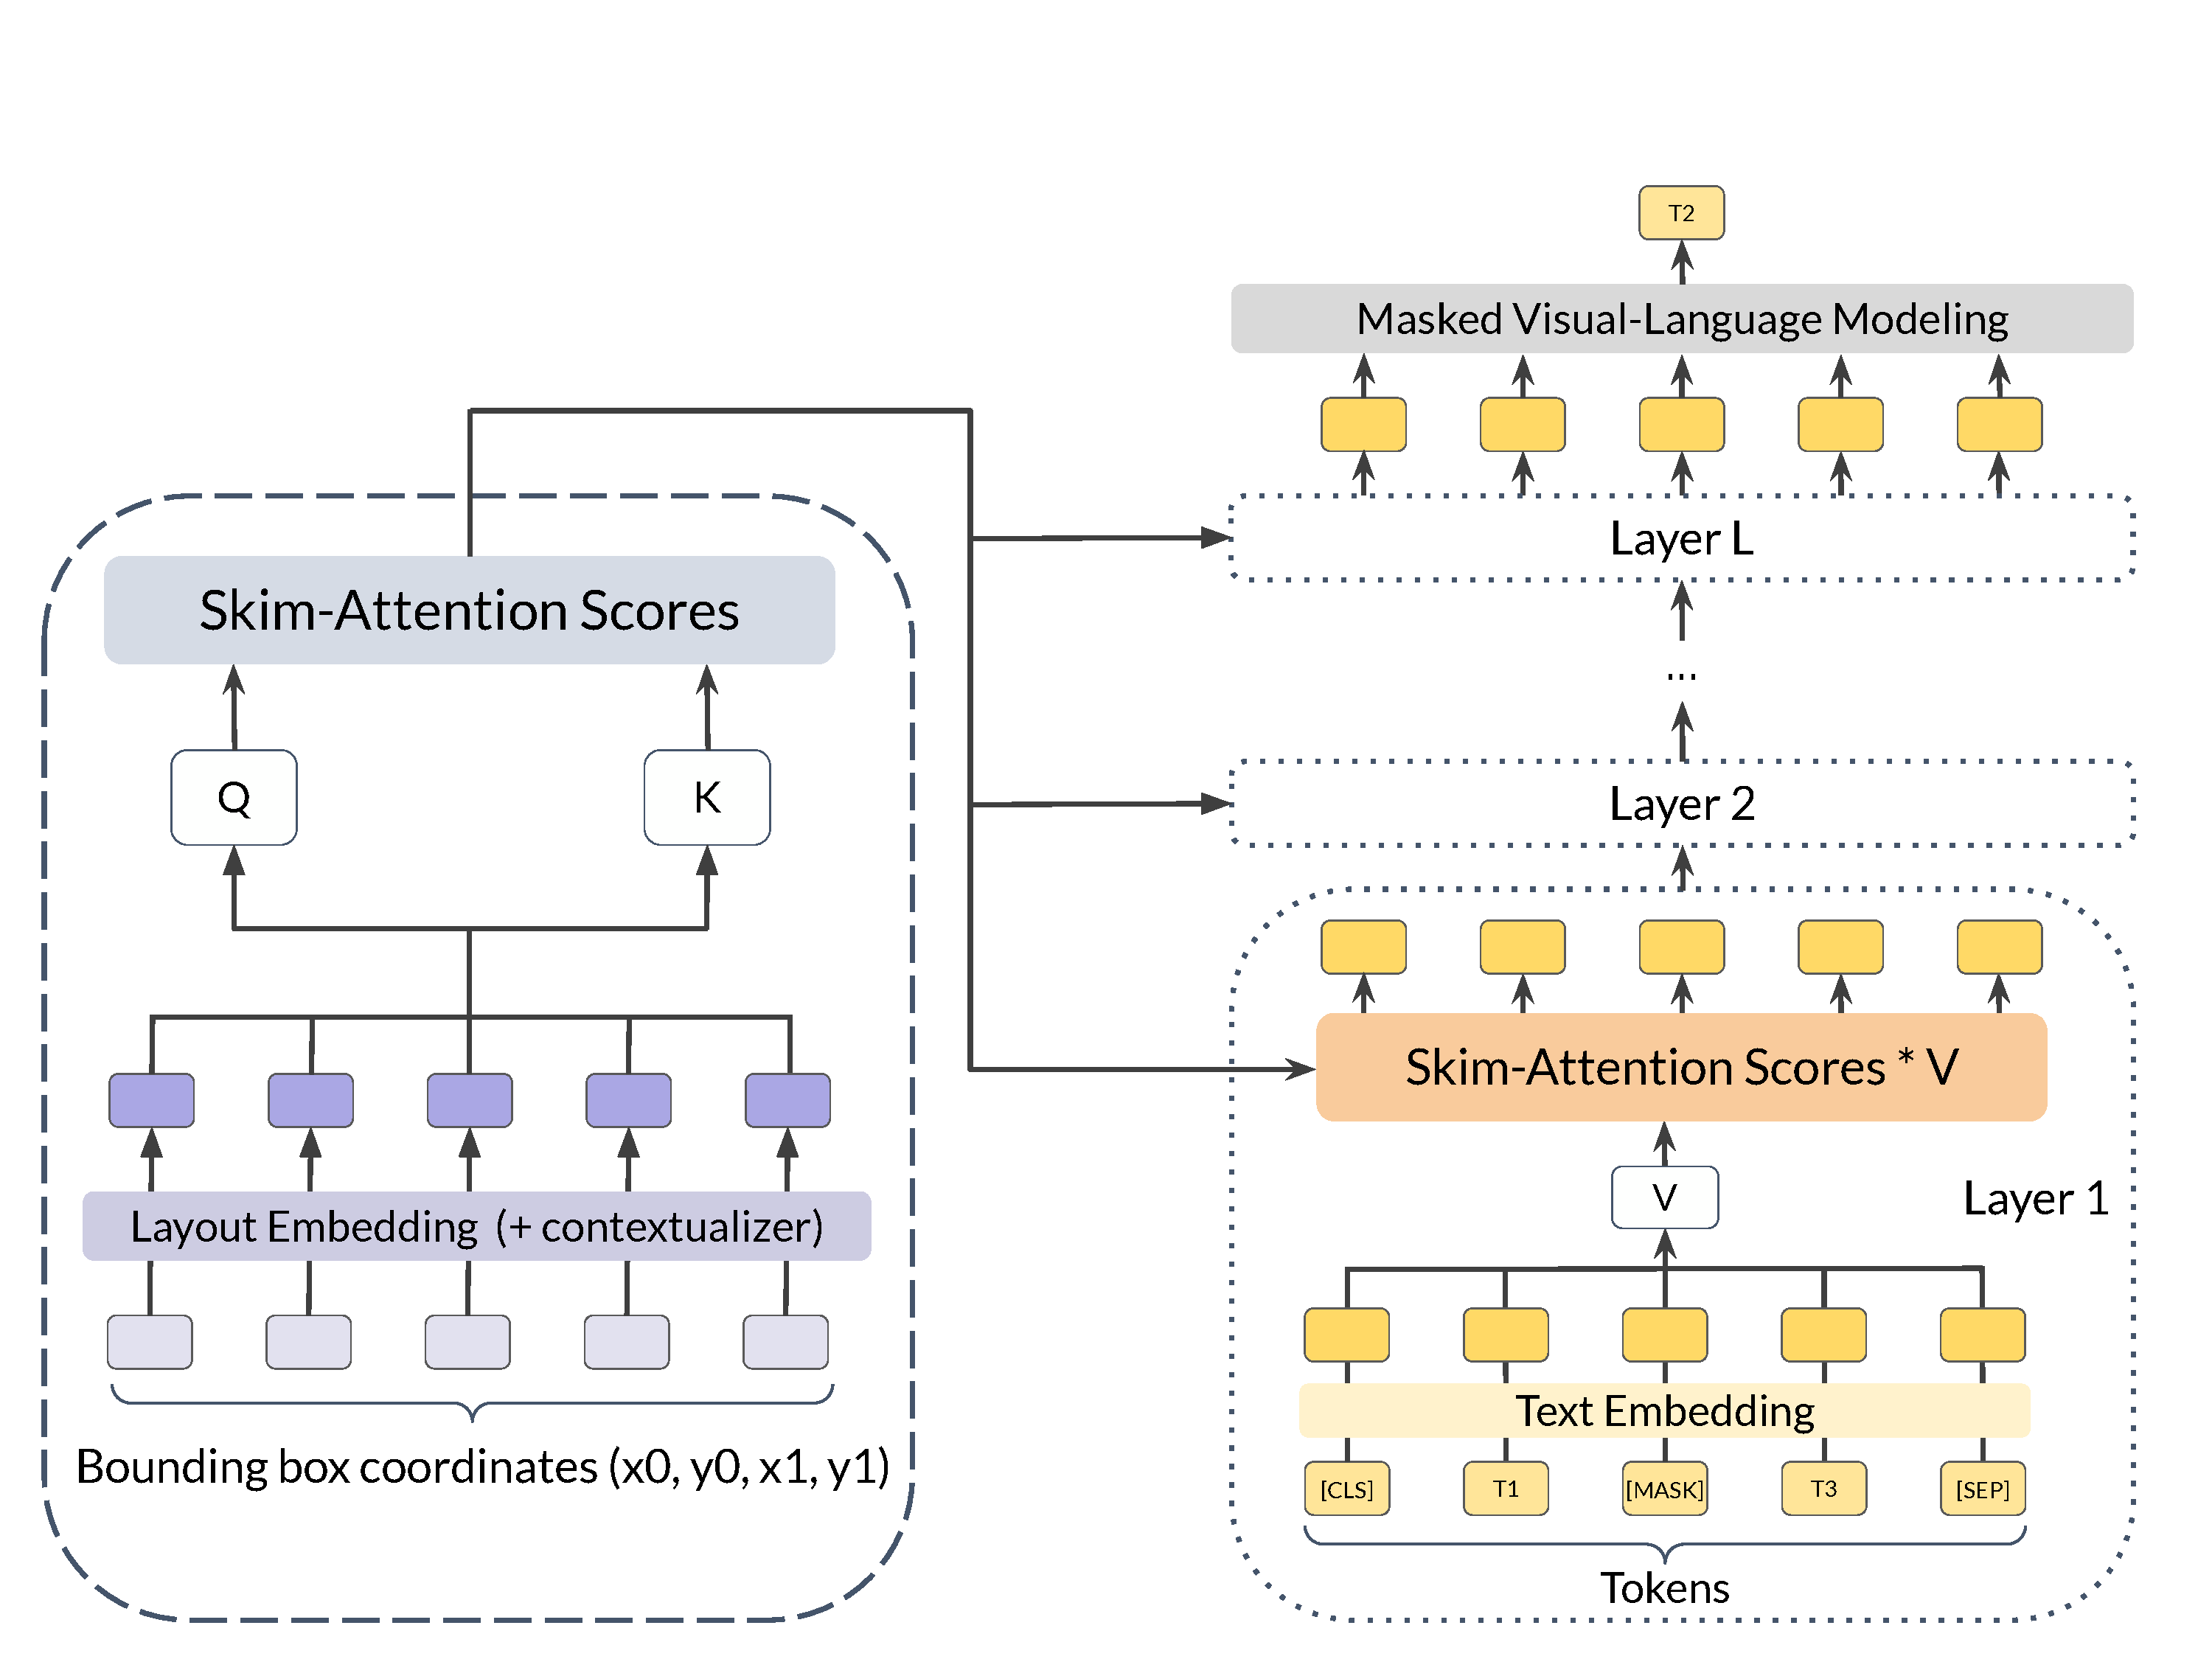
\includegraphics[width=0.7\textwidth]{images/chapter3/skimformer-architecture.pdf}
    \caption{Skimformer model architecture. The input consists of two components: a sequence of tokens and a sequence of token bounding box coordinates. Both of these sequences are transformed into corresponding embedding sequences. Only the layout embeddings are used to compute Skim-Attention. $L$ denotes the number of Transformer encoder layers. $\bm{Q}$ and $\bm{K}$ are the queries and keys obtained by projecting the layout embeddings. $\bm{V}$ represents the values produced by projecting the encoder layers' textual inputs. The attention is solely based on token spatial positions and computed only once. The attention scores are then distributed to each layer of a Transformer encoder.}
    \label{fig:chapter3-skimformer-architecture}
\end{figure}

\emph{Skimformer} is designed to answer the first research question: \textit{Is it possible to learn attention using layout only ?} Skimformer is a two-stage Transformer that replaces vanilla self-attention with Skim-Attention. Drawing inspiration from insights in cognitive science, the intuition behind this approach is to mimic how humans process a document by \emph{i)} skimming through the document to extract its structure, and \emph{ii)}  reading the contents based on the prior structural understanding. 

Skimformer is fed with a sequence of token embeddings and the corresponding sequence of layout embeddings. The model adopts a two-step approach: first, it computes the skim-attention scores once and only once using layout information alone; then it uses these attention scores across all layers of a Transformer encoder. The architecture of Skimformer is depicted in Figure~\ref{fig:chapter3-skimformer-architecture}.

For a given encoder layer $k$ and a single head, the traditional self-attention operation becomes:

\begin{equation}
\label{eq:chapter3-skim-attention-full}
	\bm{Z}'_k = \bm{A}^{\ell} \bm{V}^{t}_{k}
\end{equation}

\noindent where $\bm{A}^{\ell}$ is the skim-attention matrix obtained through Eq.~\ref{eq:chapter3-skim-attention-matrix}, and $\bm{V}^{t}_{k} = \bm{W}_{v,k} \bm{X}^t$ is the Value matrix produced by projecting the textual input $\bm{X}^t = \{\bm{t}_0, \bm{t}_1, …, \bm{t}_n\}$ at layer $k$.

More intuitively, computing skim-attention scores (Eq.~\ref{eq:chapter3-skim-attention-matrix}) can be interpreted as \textit{skimming through} the document to grasp its structural aspects. Information about the semantics (contained in $\bm{V}$) is then routed based on these similarity scores. This is done via Eq.~\ref{eq:chapter3-skim-attention-full} and can be seen as \textit{reading} the contents of the document, focusing on the most relevant parts guided by the skim-attention scores.

Similarly to LayoutLM, we pre-train Skimformer using \ac{MVLM}. This involves randomly masking some of the input tokens, while retaining their corresponding layout embeddings. The model is then trained to recover the masked tokens given the contexts. 

% As no assumption is made on the architecture of the encoder, any Transformer model can be used as the backbone of Skimformer.

While we experimented with a standard Transformer encoder-only model, it is worth noting that any language model can be used as the backbone of Skimformer.

Albeit remaining quadratic, the time and memory cost of Skim-Attention is lower than vanilla self-attention. Let $n$ be the maximum sequence length, $h$ the number of attention heads, $L$ the number of encoder layers, $d$ the dimension of the text embeddings, and $d'$ the dimension of the layout embeddings. The computational complexity is reduced from $\mathcal{O}(2Lhdn^2)$ to $\mathcal{O}(hd'n^2 + Lhdn^2)$, the first term being the time required to calculate the skim-attention scores, and the second term referring to the time needed to compute the Value matrix in each layer. The memory complexity for vanilla self-attention is $\mathcal{O}(Lhdn + Lhn^2)$, where the first term is the memory required to store keys, queries and values, while the second represents the attention scores produced. These requirements are reduced to $\mathcal{O}((hd’n + hn^2) + Lhdn)$, with the first term corresponding to the keys and queries, the second term representing the attention scores, and the last one corresponding to the values.


\subsubsection{Skimming Mask}

\begin{figure}
    \centering
    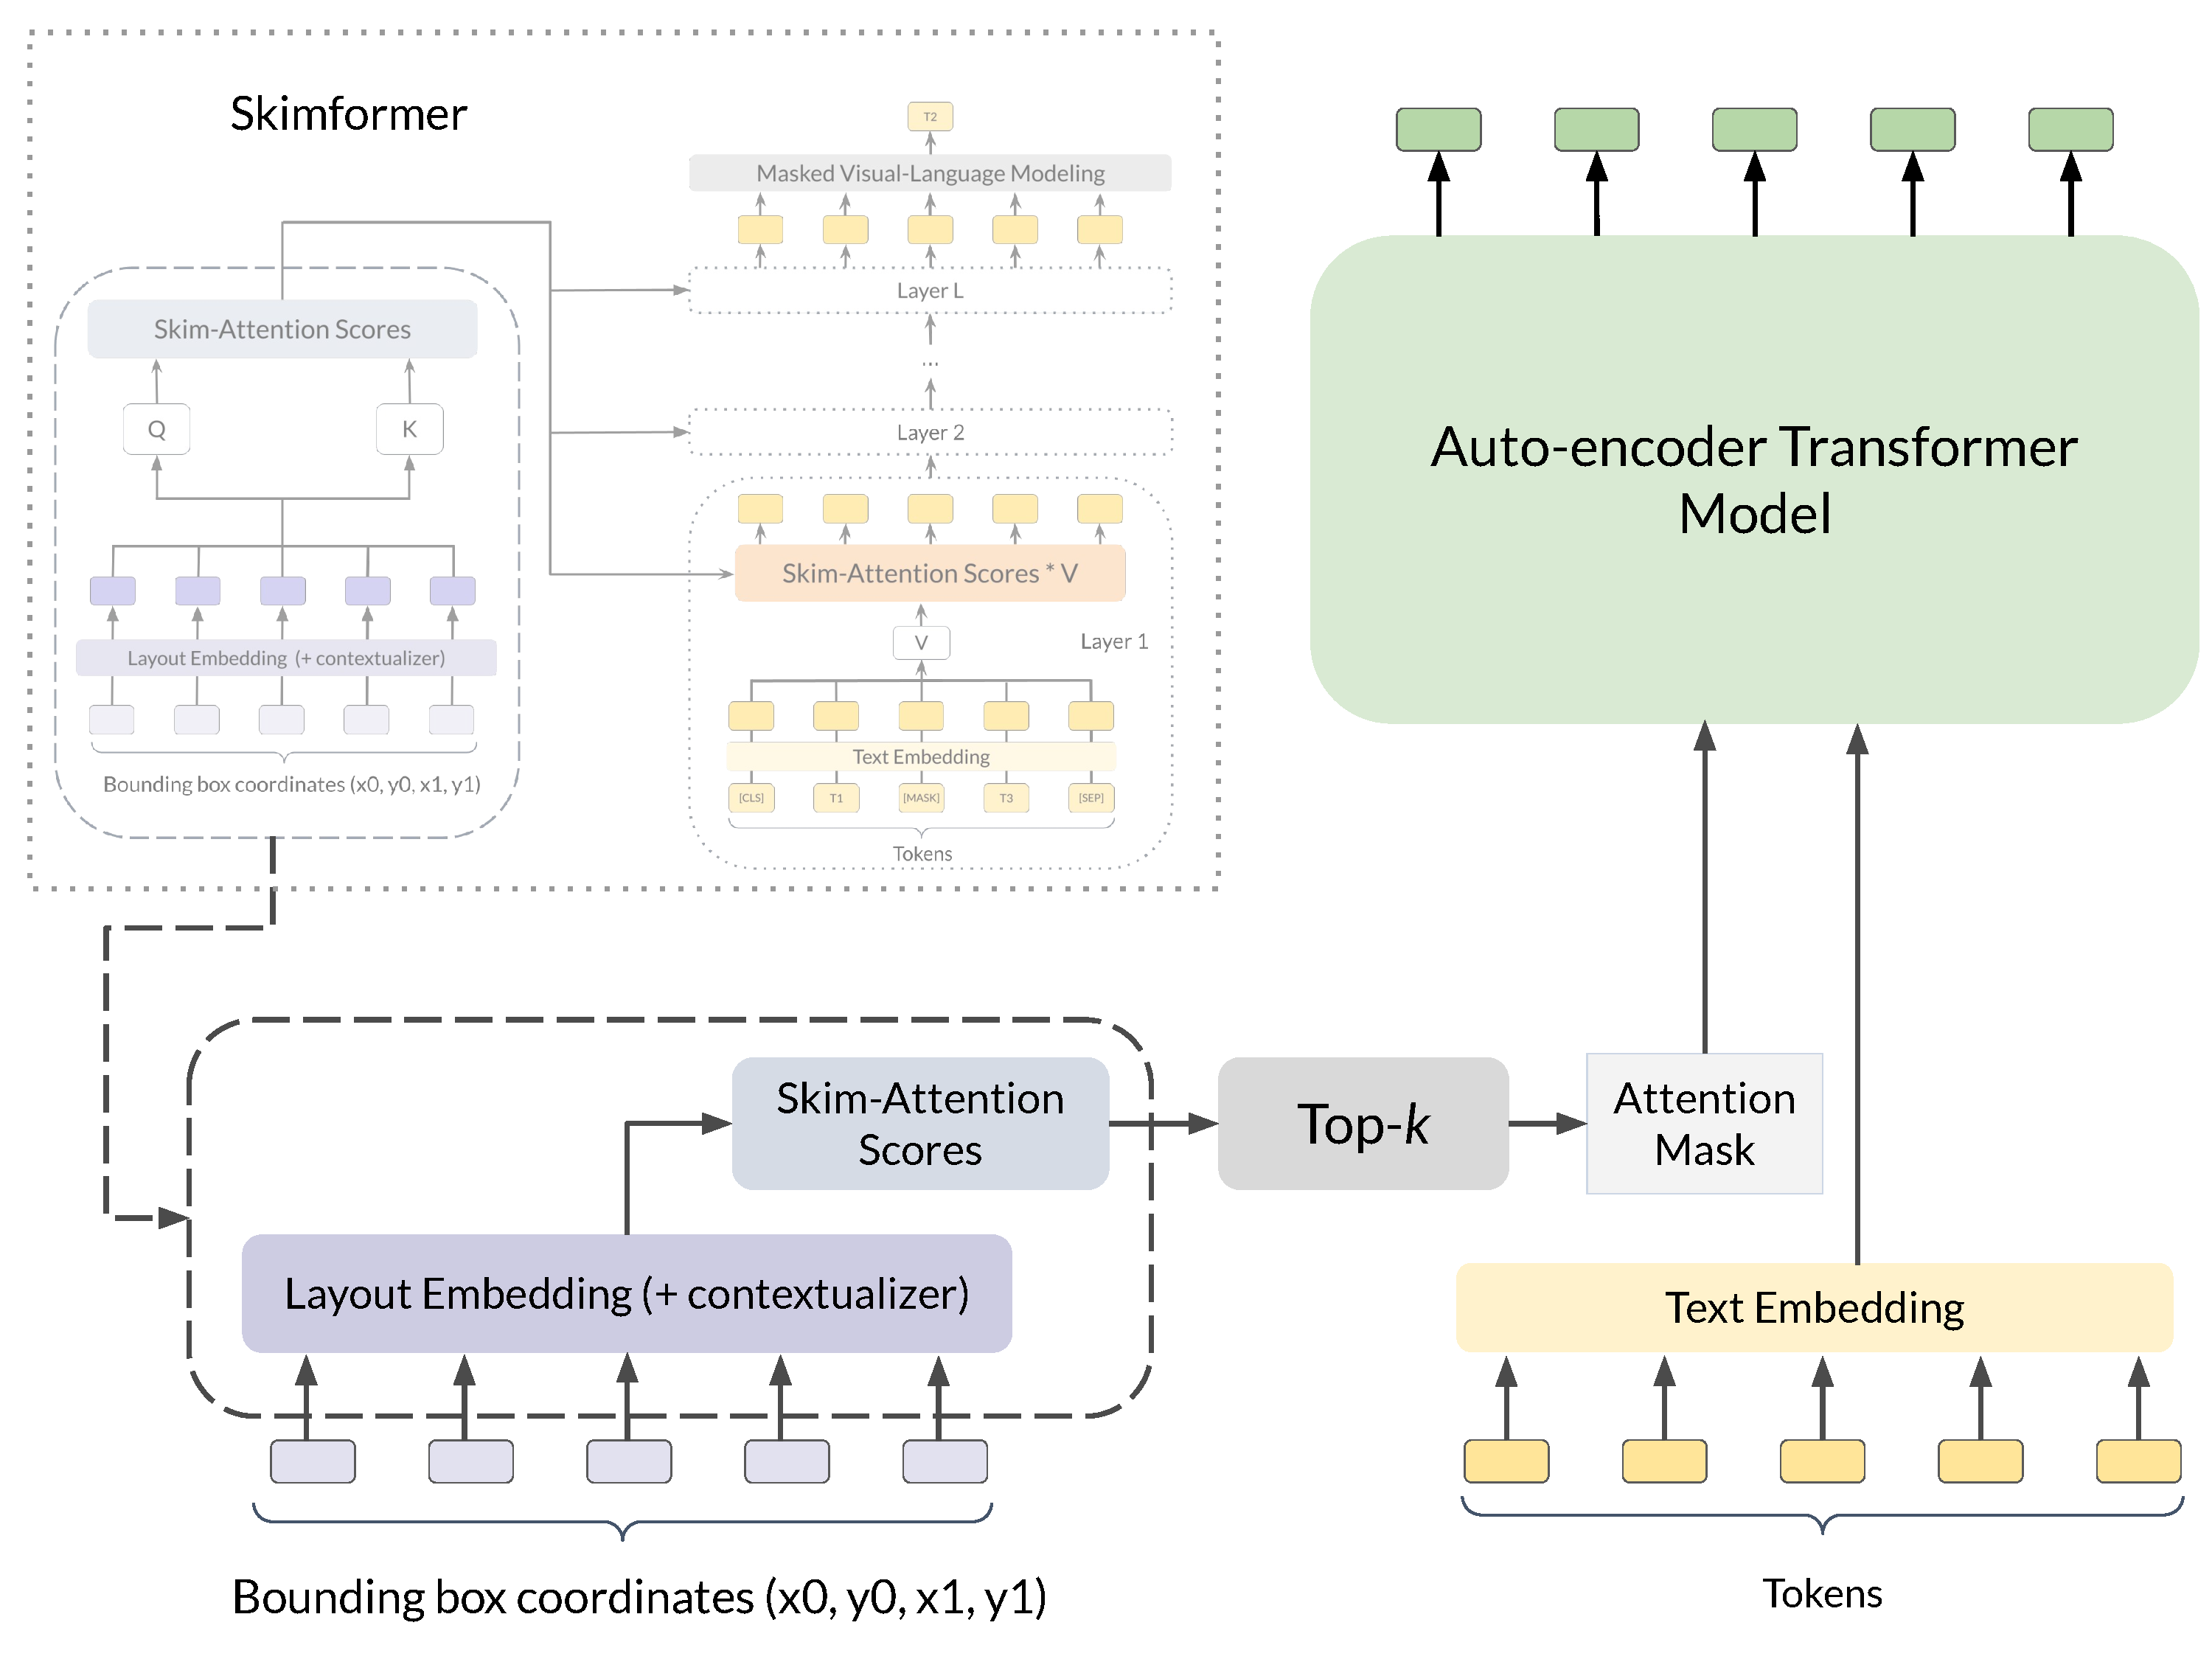
\includegraphics[width=0.7\textwidth]{images/chapter3/skimmingmask-architecture.pdf}
    \caption{Skimming Mask model architecture. The layout embeddings, Key and Query projections are initialized from an already pre-trained Skimformer model. By filtering the $k$ most attended tokens for each token, the Skim-Attention scores are then converted to an attention mask and given as input to a text-based Transformer model.}
    \label{fig:chapter3-skimmingmask-architecture}
\end{figure}

For each token in a sequence, Skim-Attention provides a ranking of every other token in accordance with their layout-based similarity. Drawing from this observation, \emph{Skimming Mask} answers the second question: \textit{Can layout help reduce the complexity of self-attention ?} by using Skim-Attention as a mask to restrict the computation of self-attention to a smaller number of elements for each token. In this setting, Skim-Attention is viewed as an independent, complementary module that can be plugged into any language model. Given a sequence of layout embeddings, the corresponding skim-attention matrix is converted to an attention mask: based on the similarity scores provided in the attention matrix, each token can only attend to its $k$ most similar tokens. The resulting mask is then given as input to a text-based Transformer language model with vanilla self-attention, and is used to restrict self-attention for each element in the input text sequence. This can be viewed as \emph{sparsifying} the vanilla self-attention matrix.

Skimming Mask cannot be trained end-to-end alongside the Transformer model it is integrated with, primarily because generating an attention mask from an attention matrix is a non-differentiable operation. Consequently, to train this model, the weights for Skim-Attention must have already undergone training. In this context, we naturally use the pre-trained Skimformer weights.  The overall architecture of the model is illustrated in Figure~\ref{fig:chapter3-skimmingmask-architecture}.

It is worth nothing that Skimming Mask introduces a new way to cluster tokens: tokens within the same group have a high similarity to each other in terms of their respective \emph{layout positions}. This characteristic positions Skimming Mask as a concurrent approach to Reformer \citep{kitaev2020reformer}, which reduces the cost of self-attention by clustering tokens into chunks. As opposed to the latter, the concept of similarity is not derived from text semantics but rather from the document structure. Furthermore, Skimming Mask does not require an understanding of the semantic content; it solely relies on their layout features. Because each token is viewed as a bounding box whose characteristics are only its size and position, the representation space of layout features is much smaller than that of the text, which spans a vocabulary of more than 30k sub-words. As a consequence, computing attention based on layout could require a smaller latent space dimension than for text, corresponding to less computational efforts. This is also the case for humans: as demonstrated in section \ref{section:chapter3-human-evaluation}, it is much easier to retrieve information from documents when the layout is provided.


\section{Experiments and Results}

We first present the data used to pre-train and evaluate our models, and provide details on the experimental settings. Then, we discuss the results obtained on \ac{MVLM} and \ac{DLA}, before exploring the attention maps obtained by Skimformer.

\subsection{Data}

\subsubsection{Pre-training Data}

To pre-train our models on a wide variety of document formats, we select three datasets with various non-trivial document layouts: DocBank \citep{li2020docbank}, RVL-CDIP \citep{harley2015evaluation} and PubLayNet \citep{zhong2019publaynet}. We combine them by randomly selecting 25k documents from each dataset, for a total of 75K documents. We discard the provided labels and consider these data as unannotated. The resulting dataset is referred to as \textit{MIX}. As a first evaluation metric, we can compare the perplexity for the different language models on MIX. 

\paragraph{DocBank}

DocBank is a large-scale dataset that contains 500K English document pages from papers extracted from arXiv.com. These articles span a variety of disciplines (\textit{e.g.}, Physics, Mathematics, and Computer Science), which is beneficial to train more robust models. Pages are split into a training set, validation set and test set with a ratio of 8:1:1. As the authors already extracted the text and bounding boxes using PDFPlumber,\footnote{https://github.com/jsvine/pdfplumber} there is no need for an OCR system or a PDF parser. To build our subset, we extract 25k document pages: 20k from the full training set, 2,500 from the validation set and 2,500 from the test set. 

\paragraph{RVL-CDIP}

RVL-CDIP is a large collection of 400k scanned document images from various categories (\textit{e.g.}, letter, form, advertisement, invoice). The wide range of layouts, as well as the low image quality, allows to train more robust models. We select 25k documents from the RVL-CDIP dataset available on Kaggle,\footnote{https://www.kaggle.com/nbhativp/first-half-training} which amounts to half of the training images from the full dataset (160k images). The text and word bounding boxes are extracted using Tesseract.\footnote{https://github.com/tesseract-ocr/tesseract} We split the data into 80\% for training, 10\% for validation and 10\% for test.

\paragraph{PubLayNet}

PubLayNet comprises over 360 thousand document images from PubMed Central\textsuperscript{\texttrademark} Open Access. The medical publications contained in the collection have similar layouts, but the text density coupled with the small image size add to the robustness of the trained models. We extract the first training split among the 7 available on IBM Data Asset eXchange\footnote{https://developer.ibm.com/exchanges/data/all/publaynet/} and use the first 20k images as our training set. For the validation and test sets, we keep the first 2,500 images in each split. Because OCR accuracy is too low without any pre-processing, we apply a few image processing operations (\textit{i.e.}, rescaling, converting to grayscale, applying dilation and erosion) on each image in order to improve text extraction.

\subsubsection{Dataset for Document Layout Analysis}

In addition to perplexity, we evaluate our approach on a downstream task, \ac{DLA}, which consists in associating each token with its corresponding category. We use a subset of the full DocBank dataset, where the categories are: abstract, author, caption, date, equation, footer, list, paragraph, reference, section, table, title and figure.\footnote{We actually discard the \textit{Figure} label, as 1) our models do not take image features into account, and 2) the text associated with such elements is always the same, making the task trivial.}

The subset is created by selecting 10k document pages (distinct from the ones used for pre-training): 8,000 from the full training set, 1,000 from the validation set and 1,000 from the test set. We refer to this dataset as \textit{DocBank-LA}. Each document page is organized as a list of words with bounding boxes, colors, fonts and labels. We use the precision, recall and F1 score defined by \citet{li2020docbank}.

\subsection{Experimental Settings}

For reproducibility purposes, the code and data pre-processing scripts are made publicly available.\footnote{https://github.com/recitalAI/skim-attention}

\subsubsection{Baselines}

We compare our models with three baselines: i) the text-only \ac{BERT}, ii) the multi-modal LayoutLM, and iii) the text-only Longformer for long documents. Note that the LayoutLM architecture is based on \ac{BERT}, with additional layout components. For fair comparison, all our models designed for short sequences are based on \ac{BERT} as well, as detailed below.

\subsubsection{Pre-training}

For \ac{BERT}, LayoutLM and Longformer, we use their default architecture. Following the \ac{BERT} base model, Skimformer consists of a 12-layer Transformer encoder with 12 attention heads and a hidden size set to 768 for both text and layout embeddings, amounting to 99M parameters. We further add a 2-layer Transformer encoder to contextualize the layout embeddings, which increases the number of parameters to 113M. To test Skim-Attention on longer documents, we build LongSkimformer, a combination of Skim-Attention and Longformer. Every model is trained from scratch on the MIX dataset for 10k steps. We set the maximum sequence length to $n = 512$ for every model except for Longformer and LongSkimformer, for which $n = 2,048$. Skimformer, LongSkimformer and LayoutLM are pre-trained using MVLM, while \ac{BERT} and Longformer are pre-trained with MLM.

\subsubsection{Document Layout Analysis}

As DocBank contains fine-grained token-level annotations, we consider the document layout analysis task as a sequence labeling task. Each model pre-trained on MIX is fine-tuned on this downstream task for 10 epochs. For the Skimming Mask models, we selected the hyperparameter $k$ on validation, i.e. the number of tokens that can be attended to. We tested $k \in [512, 384, 256, 128]$.

\subsection{Language Modeling Evaluation}

\subsubsection{Perplexity}

\begin{table}
\centering \small
\begin{tabular}{lr}
    \hline
    \textbf{Model} & \textbf{Test Perplexity}\\
    \hline
    \ac{BERT} \citep{devlin2018bert} &  357.11 \\
    LayoutLM \citep{xu2020layoutlm}    & 45.86 \\
    Skimformer                         & 33.77 \\
    \midrule
    Longformer \citep{beltagy2020longformer} & 333.28 \\
    LongSkimformer                     & \textbf{32.02} \\
    \hline
\end{tabular}
\caption{Test perplexity on the MIX dataset after 10k optimization steps. Each model was trained from scratch. Bold denotes the best score.}
\label{tab:chapter3-ppl-mix}
\end{table}

In Table~\ref{tab:chapter3-ppl-mix}, we report the perplexity on the MIX dataset. We observe that Skimformer and LongSkimformer outperform both \ac{BERT} and Longformer by a huge margin, while improving perplexity by more than 10 points over LayoutLM. In addition, Figure~\ref{fig:chapter3-pretraining-learning-curves} demonstrates that Skimformer converges much faster than \ac{BERT}, and slightly more than LayoutLM.

\begin{figure}
    \centering \small
    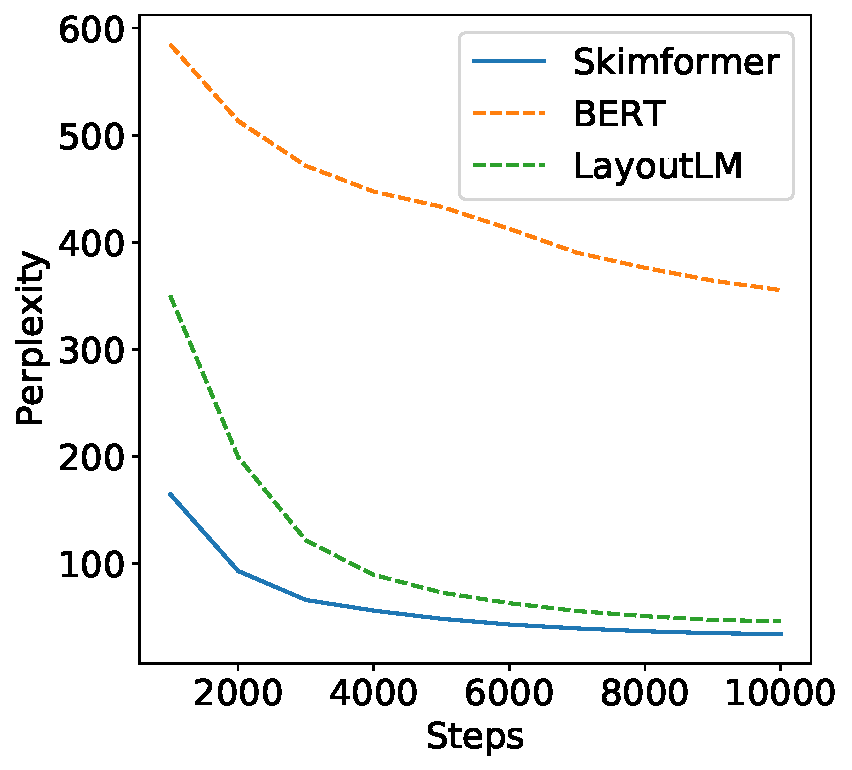
\includegraphics[width=.4\textwidth]{images/chapter3/learning_curves-mix-steps10k-clean2.pdf}
    \caption{Model perplexity on the MIX validation set with respect to the number of optimization steps. All models are trained from scratch.}
    \label{fig:chapter3-pretraining-learning-curves}
\end{figure}

\subsubsection{Ablation Study}

We further conduct an ablation study about the influence of the Skim-Attention inputs on Skimformer's performance. The results are listed in Table~\ref{tab:chapter3-ablation-study}. To estimate the impact of the input type, we consider a Skimformer model i) wherein Skim-Attention is based on sequential positions (\textit{1D position}), ii) the bounding boxes are all set to the same fixed value, preventing the model to gather any information about the true location (\textit{Uniform layout}), iii) they are replaced by their centers (\textit{Degraded layout}), and iv) the layout embeddings are contextualized (\textit{Contextualized Layout}). 

\begin{table}[t]
\centering \small
\begin{tabular}{lr}
    \hline
    \textbf{Skim-Attention Input} & \textbf{Test Perplexity}\\
    \hline
    Layout                              & 36.41 \\
    1D position                         & 54.39 \\ 
    Uniform layout                      & 421.97 \\
    Degraded layout                     & 103.39 \\
    Contextualized layout               & \textbf{33.77} \\
    \hline
\end{tabular}
\caption{Ablation study on the MIX dataset, where perplexity on the test set is reported. All models were trained from scratch. Bold denotes the best score.}
\label{tab:chapter3-ablation-study}
\end{table}

We can see that replacing spatial with sequential positions results in an increase in perplexity, indicating that layout information is crucial for the Language Model. It is also observed that assigning the same bounding box to every token leads to a severe drop in performance. Coupled with the perplexity obtained with a degraded layout, this shows that the model's performance is greatly impacted by the layout input quality. At last, contextualizing the layout inputs through a small Transformer brings slight improvements over computing Skim-Attention directly on the layout embeddings.

\subsubsection{Training Speed and Memory Usage}

Using Hugging Face's Transformers benchmarking tools \citep{wolf2019huggingface}, we benchmark Skimformer and LayoutLM on both speed and required memory for pre-training. We consider the base variant of LayoutLM, and use the implementation from the Transformers library. In addition to the full Skimformer, we evaluate a variant in which the small Transformer contextualizing layout embeddings is removed (\textit{Skimformer-no-context}). The batch size is fixed to 8, and memory and time performance is evaluated for the following sequence lengths: 8, 32, 128 and 512. All experiments were conducted on one Tesla T4 with 15GB of RAM.

% We use Python 3.7.10, PyTorch 1.8.1+cu101 \citep{paszke2019pytorch}, and Transformers 4.6.0.dev0.

Figures~\ref{fig:chapter3-benchmark-train-time} and \ref{fig:chapter3-benchmark-train-memory} report the time and peak memory consumption, respectively, with respect to the sequence length. Results show that Skimformer is more time and memory efficient than LayoutLM. 

\begin{figure}[!htbp]
\centering
\small
  \begin{subfigure}[b]{0.49\textwidth}
    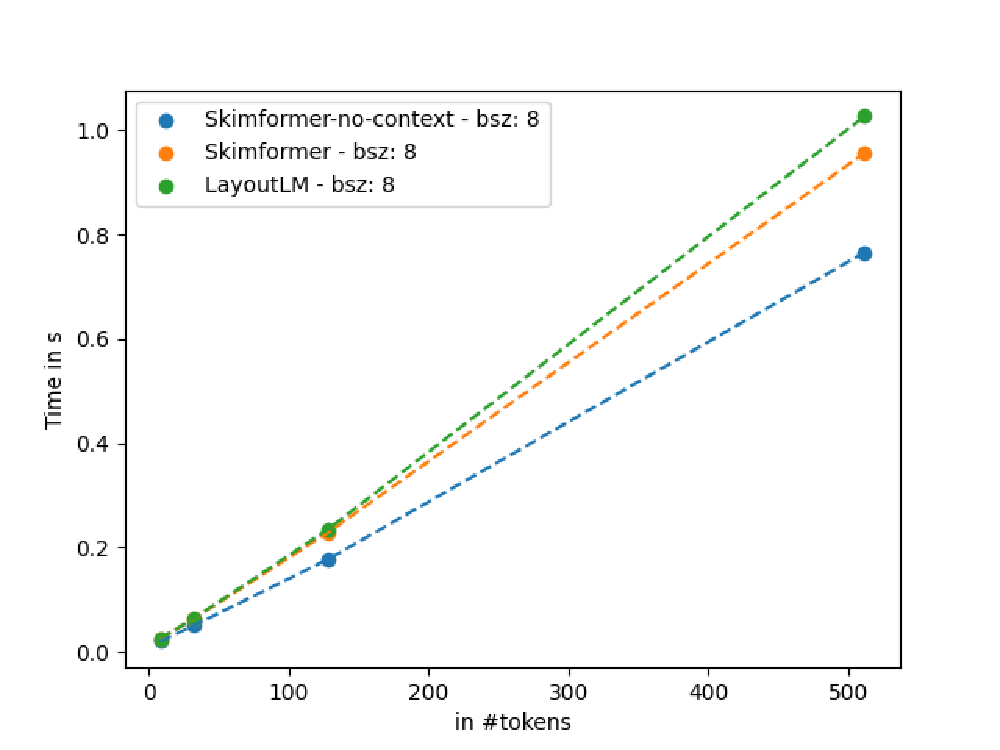
\includegraphics[width=\textwidth]{images/chapter3/train_time_plot.pdf}
    \caption{Time usage for pre-training.}
    \label{fig:chapter3-benchmark-train-time}
  \end{subfigure}
  \begin{subfigure}[b]{0.49\textwidth}
    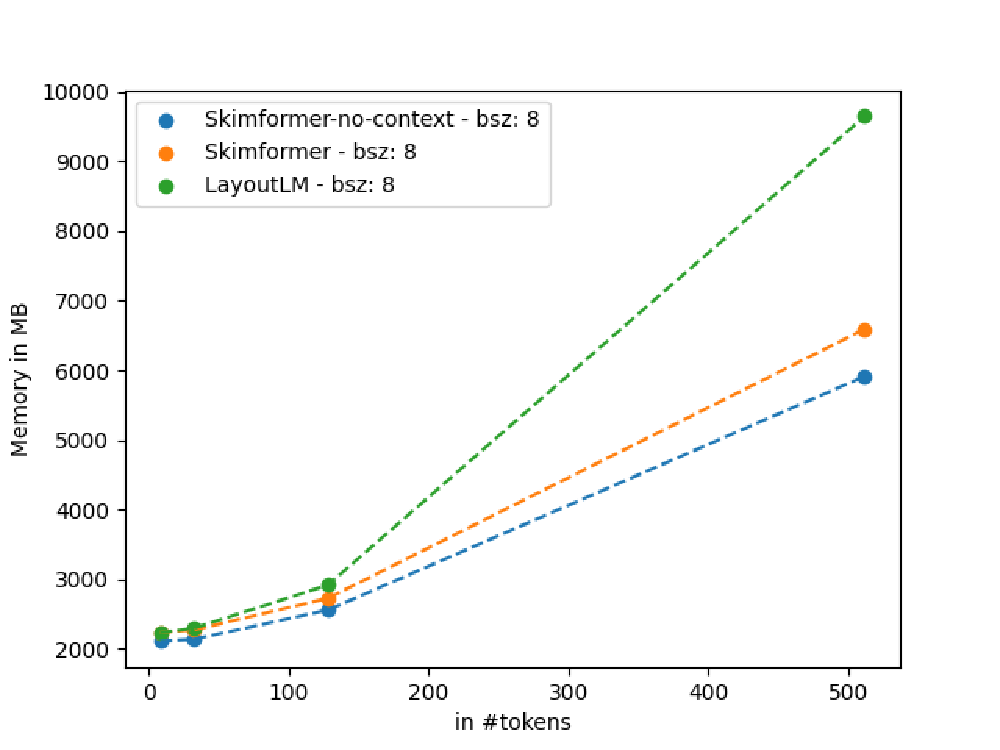
\includegraphics[width=\textwidth]{images/chapter3/train_required_memory_plot.pdf}
    \caption{Memory usage for pre-training.}
    \label{fig:chapter3-benchmark-train-memory}
  \end{subfigure}
  \caption{Comparison of time and memory usage for LayoutLM (green), Skimformer with layout contextualizer (orange) and without (blue). Results are plotted against sequence length.}
  \label{fig:chapter3-benchmark}
\end{figure}

\subsection{Document Layout Analysis Evaluation}

\begin{table}
\centering
\small
\begin{adjustbox}{max width=\textwidth}
\begin{threeparttable}
\begin{tabular}{lcccccccc}
    \toprule
     & \textbf{Skimming} & \textbf{Seq.} & \multicolumn{2}{c}{\textbf{Nb Attentions}} & \textbf{Total} & & & \\
    \textbf{Model} & \textbf{Mask} & \textbf{Len} & \textbf{Original}\tnote{*} & \textbf{Skim-Attn} & \textbf{Compute} & \textbf{Rec.} & \textbf{Prec.} & \textbf{F1} \\
    \midrule
    BERT \citep{devlin2018bert}  & \xmark                         & 512 & 12              & 0 & 100.00\% & 67.21 & 59.28 & 60.98 \\ 
    LayoutLM \citep{xu2020layoutlm}        & \xmark                         & 512 & 12              & 0 & 100.00\% & 81.60 & 77.96 & \textbf{79.28} \\
    \midrule 
    Skimformer          & \xmark                         & 512 & 0 & 3\tnote{**} & 25.00\% & 78.80 & 74.35 & 75.86 \\
    BERT+SkimEmbeddings & \xmark                         & 512 & 12              & 0 & 100.00\% & \textbf{82.42} & 77.06 & \textbf{79.16} \\
    
    BERT+SkimmingMask                & \cmark  & 128  & 12  & 3\tnote{**} & 31.25\% & 72.32 & 64.39 & 67.36 \\
    LayoutLM+SkimmingMask              & \cmark & 128 & 12 & 3\tnote{**} & 31.25\% & 81.15 & \textbf{78.30} & \textbf{79.26} \\ 
    \midrule 
    Longformer \citep{beltagy2020longformer} & \xmark & 2,048 & 12 & 0 & 100\% & 74.88 & 69.29 & 71.17 \\
    LongSkimformer & \xmark & 2,048 & 0 & 3\tnote{**} & 25\% & 81.22 & 73.45 & 76.61 \\
\bottomrule
\end{tabular}
\begin{tablenotes}
  \item[*] Standard self-attention for Skimformer, BERT-based and LayoutLM-based models. Longformer self-attention for Longformer and LongSkimformer.
  \item[**] Attention is computed twice (by a 2-layer Transformer) during layout contextualization, then once by Skim-Attention.
\end{tablenotes}
\end{threeparttable}
\end{adjustbox}
\caption{Model performance (in \%) on the DocBank-LA dataset. \textit{Seq. Len} indicates the number of tokens attended with either standard attention (for Skimformer, BERT-based and LayoutLM-based models), or Longformer attention (for Longformer and LongSkimformer). \textit{Nb Attention} represents the number of times attention (original and Skim-Attention) is computed and stored. \textit{Total Compute} specifies the ratio of the final computational cost (\# operations needed to compute attention) w.r.t. BERT/LayoutLM or Longformer. Each model was pre-trained from scratch on MIX, then fine-tuned on DocBank-LA. }
\label{table:chapter3-results-docbank}
%\vspace{-0.5cm}
\end{table}

Table~\ref{table:chapter3-results-docbank} reports the performance on DocBank-LA, the sequence length processed, the number of times attention is computed and the ratio of the total calculation unit ($n^2 \times \textrm{Nb Skim-Attn} + \textrm{Seq. Len}^2 \times \textrm{Nb Standard Attn}$, where $n$ is the length of the initial sequence on which Skim-Attention is applied; and \textit{Seq. Len} is the length obtained after applying Skimming Mask) to that of \ac{BERT}/LayoutLM and Longformer. All models were pre-trained from scratch on MIX. 

Skimformer is substantially superior to \ac{BERT}, improving the F1 score by 15\% while reducing the number of attentions computed by four. We experimented with plugging the layout embeddings learnt by Skimformer in a \ac{BERT} model. The resulting model, BERT+SkimEmbeddings, resembles LayoutLM in terms of architecture.\footnote{In BERT+SkimEmbeddings, the layout embeddings are first projected into the same dimensional space as the text embeddings. In this way, we can plug the layout embeddings from any Skimformer model, in particular smaller ones.} Results show that BERT+SkimEmbeddings performs on par with LayoutLM despite simply combining separately pre-trained modalities, as opposed to the latter which requires an extensive joint training.

For the Skimming Mask models (see the last two rows in Table~\ref{fig:chapter3-results-docbank}), the models attend to only the top-$k$ 128 tokens. Compared to LayoutLM, this reduction to the quadratic factor allows to obtain the same downstream results with only 31.25\% of the computational burden.
Compared to \ac{BERT}, it even obtains an absolute improvement of more than 6\% in term of F1 score.

LongSkimformer benefits from both Skim-Attention and Longformer's gain in efficiency. It outperforms Longformer by 5\% while requiring four times less attention operations, and the use of Longformer's linear attention allows LongSkimformer to process sequences four times larger than Skimformer can.

\subsection{Attention Visualization}

\begin{figure}
    \centering \small
    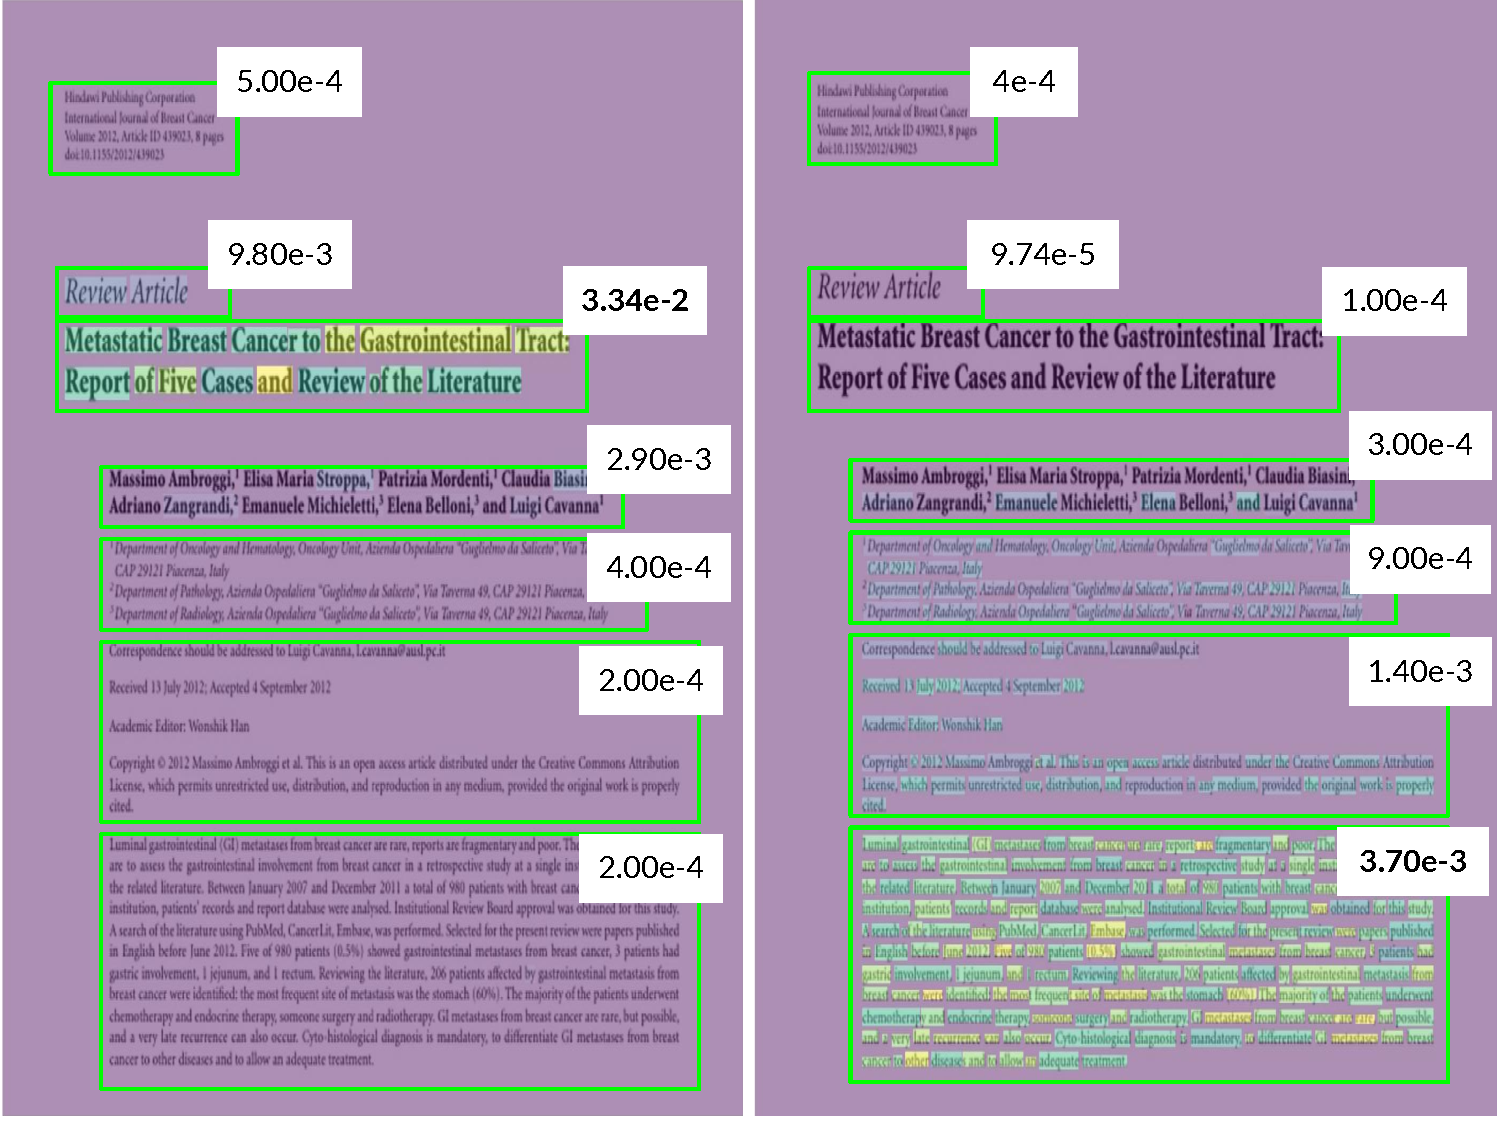
\includegraphics[width=.49\textwidth]{images/chapter3/attention-maps_with-average.pdf}
    \caption{Skim-attention maps corresponding to the title (left) and the abstract (right), along with average attention score (in white) per text block (in green). We consider the skim-attention matrix averaged over all the attention heads. Given a semantic unit (title or abstract), we plot the average attention score for each token.
    }
    \label{fig:chapter3-attention-vis}
    % \vspace{-0.5cm} 
\end{figure}

Figure~\ref{fig:chapter3-attention-vis} shows the attention maps produced by Skimformer on a randomly sampled document. Given a semantic unit (either title or abstract in our example), we select the corresponding tokens and compute their average attention over the whole document. We observe, both qualitatively and quantitatively, that tokens attend mainly to other elements in the same semantic unit, thus creating clusters of tokens that are relevant to each other. This shows that the model has grasped the concept of semantic unit with only self-supervision, enabling the emergence of a document structure representation. We argue that these structure-aware clusters could pave the way for long text encoding and unsupervised document segmentation.

\section{Conclusion}

We have presented Skim-Attention, a novel structure-aware attention mechanism. Distinct from prior works in layout-aware pre-training, Skim-Attention builds on cognitive science: rather than reading every single word in the document to compute attention, our approach exploits the 2D positions of the words. We conduct extensive experiments to show the effectiveness of Skim-Attention, both as an end-to-end model (Skimformer) and as a mask for any language model (Skim-Attention).

Potential extensions of this work include integrating image features into Skim-Attention to leverage information across all modalities, as well as exploring tasks that require capturing longer-range dependencies.





	\cleardoublepage
	\let\leftmark=\oldleftmark

	\acresetall
	
\chapter{Addressing Serialization Errors by Discarding Sequential Position Information}
\label{chapter:chapter4}

\renewcommand{\leftmark}{\spacedlowsmallcaps{Addressing Serialization Errors by Discarding Sequential Position Information}}

\begin{chapabstract}
    {\em
    Chapter Abstract


    \vspace*{5mm}
    The work in this chapter has led to the submission of a paper currently under review:}
    \begin{itemize}
        \item \small \fullcite{}.
    \end{itemize}
\end{chapabstract}

\ifthenelse{\boolean{skipCh4}}{\endinput}{}


\newpage

\minitoc
\chapterwithfigures{\nameref*{chapter:chapter4}}
\chapterwithtables{\nameref*{chapter:chapter4}}

Textual content is organized in a specific order to convey meaning and context. Hence, reading order is crucial for models to perform well because it reflects the natural flow and structure of information in a document. When models are trained with a reading order that aligns with human understanding, they learn to capture the relationships between words, sentences, and paragraphs. 

% it is non-trivial to obtain proper reading orders from document images due to various formats, e.g., tables, multiple columns, and most OCR engines fail to provide the proper reading order.

Most pre-training methods for Document Understanding rely on serialized text, where either an \ac{OCR} engine or a PDF parser is used to extract text. However, due to the variety of layout formats, most \ac{OCR} engines and PDF parsers struggle to provide accurate reading orders, introducing \textit{serialization errors}. Serialization errors, \textit{i.e.}, noise that may arise during text extraction, such as misinterpretations or omissions, can lead to misalignments between the extracted text and the original visual content. For instance, an \ac{OCR} engine might misinterpret or introduce extraneous characters, while a PDF parser might misinterpret formatting elements or misorder words. Most of the time, the text extracted is re-arranged in a raster-scan order, aligning tokens from the top-left to the bottom-right corner \citep{clausner2013significance}. However, this linear organization does not always align with human reading patterns, particularly in documents with complex layouts such as multicolumn texts, tables, and forms. Serialization errors impact the accuracy of the extracted text and, therefore, affect the entire text processing pipeline. Without an accurate reading order, models may misinterpret the relationships between different parts of the text, resulting in suboptimal performance in downstream tasks. This poses a substantial challenge in various applications, notably Document Understanding, where document layouts can be complex. 

Furthermore, in real-word scenarios, documents may be processed by various \ac{OCR} engines for different reasons such as cost, availability, or integration with existing workflows. Each \ac{OCR} engine may have unique characteristics related to layout, font handling, or language support, introducing variations in the quality and accuracy of the \ac{OCR} output for the same document. This variability may result in significant fluctuations in downstream performance. However, it is crucial for organizations to be able to choose \ac{OCR} engines based on their specific requirements without compromising performance in downstream tasks.

% Furthermore, inaccuracies in \ac{OCR} outputs often require manual correction, which can be time-consuming and resource-intensive.

In particular, in visual information extraction tasks, where the goal is to recognize word sequences in a document as entities of predefined semantic types (\textit{e.g.}, names, dates, addresses), performance is significantly affected by serialization errors. Following the classic settings of \ac{NLP}, the task is commonly framed as a sequence-labeling problem. This approach involves labeling
each token using a tagging scheme, such as BIO-tagging \citep{ramshaw1999text}, and leveraging these tags to identify entities. A sequence labeling-based approach operates under the assumption that each identified segment of an entity forms a continuous sequence of words within the input. While this assumption is valid for plain texts, it may not hold for real-world documents, where \ac{OCR} systems or PDF parsers might not correctly recognize and organize text. For instance, an entity might be split into non-continuous fragments. Such disordered input leads to significant confusion in the BIO-tagging scheme, preventing the models from accurately identifying entities.

On the other hand, layout inherently encapsulates the correct reading order of documents by visually organizing content in a structured manner. A well-designed layout guides the reader's natural progression from one section to another, ensuring coherent and logical information flow. Therefore, understanding the layout provides essential cues for determining the correct reading order, as it aligns with the visual hierarchy and structure intended by document creators. 

Yet, existing pre-training methods for Document Understanding often neglect this aspect, opting to oversimply the integration of layout by adding it as an extra embedding in the input layer \citep{xu2020layoutlm} or as a bias term in the attention layer \citep{xu2020layoutlmv2}. While ERNIE-Layout \citep{peng2022ernie} learns the relationship between layout and reading order through a pre-training strategy involving reading order prediction, it continues to rely on sequential position embeddings derived from the reading order obtained via \ac{OCR}. However, \citet{haviv2022transformer} show that causal language models that do not use explicit positional encodings develop an implicit understanding of absolute positions, compensating for missing information. It is suggested that causal attention allows the model to estimate the number of predecessors each token can attend to, approximating its absolute position. Our objective is to show that this can be a general case (\textit{i.e.}, with bidirectional attention) when layout information is provided.

% In particular, Visual Information Extraction heavily relies on the detected text and reading order provided by \ac{OCR}. Inaccuracies in the reading order can disrupt the structure of the extracted data, leading to issues such as entities being split into non-contiguous fragments. Besides, the task is commonly framed as a sequence labeling task, and common labeling schemes used to annotate entities in a sequence for sequence labeling, such as the BIO-tagging scheme \citep{ramshaw1999text}, entirely depend on the detected reading order. Furthermore, in the context of sequence labeling, the model's output is restricted to the detected words. As a consequence, there might be no exact match for the expected value in a document. 

In this chapter, we focus on mitigating serialization errors by entirely discarding sequential position information. We introduce \textit{Layout2Pos}, a novel module designed to generate 1D position embeddings from the document layout by learning to reconstruct the relative order between tokens. Our endeavor is twofold: from a practical standpoint, we aim to enhance the robustness of models to reading order changes, crucial for real-world applications; from a theoretical perspective, we demonstrate that it is feasible to discard sequential position information without compromising overall performance. We incorporate this module into sequence-to-sequence models for visual information extraction tasks. This integration eliminates the reliance on reading order and enables the generation of values that are not explicitly present in the input during entity extraction.


\section{Reconstructing Positional Information from 2D Positions}

In this section, we present preliminary experiments that underscore the limitations inherent in OCR outputs in terms of accurately preserving the reading order of tokens. In response to the challenges posed by OCR-induced serialization errors, we introduce a novel approach named Layout2Pos. This module goes beyond conventional approaches by discarding the reliance on reading order information. Instead, Layout2Pos leverages the inherent 2D positional information of tokens within the document page to reconstruct sequential positional information, thereby enhancing the robustness and reliability of downstream tasks.

\subsection{Preliminary Experiments: OCR Serialization Errors}

To gauge the extent of \ac{OCR}-induced serialization errors, we conduct preliminary experiments comparing the annotated ground-truth reading order against the reading orders produced by 1) Tesseract OCR \citep{kay2007tesseract}, a widely-used \ac{OCR} engine, and 2) DocTR \citep{doctr2021}, an \ac{OCR} engine based on deep learning models. The goal is to assess the alignment of the reading order produced via \ac{OCR} with the actual human reading patterns.

We use a subset of 100 documents from the ReadingBank \citep{wang2021layoutreader} dataset. ReadingBank is a benchmark dataset for reading order detection that includes high-quality reading order annotations extracted from Word documents. These annotations capture the correct sequence of words as visually presented in the documents. For our analysis, we categorize the document layouts into four types observed in the samples: \textit{plain} layout, \textit{lists}, \textit{multicolumn} layout, and \textit{tables}. We provide examples in Figure~\ref{fig:layout-examples}.

Tesseract OCR and DocTR are employed to extract and serialize text from the documents. The reading orders produced are compared against the ground-truth for discrepancies. Specifically, we evaluate accuracy by comparing, for each word in the ground-truth sequence, the actual next word with the next word in the sequence generated by each \ac{OCR} engine. We compute the accuracy obtained by each system for each specific layout type. Results are reported in Table~\ref{table:ocr-preliminary-experiments}. Our findings indicate that both \ac{OCR} engines face increased difficulty in reconstructing the correct reading order as the document layout becomes more complex.\footnote{This difficulty in accurately predicting the next word is further attributed to the \ac{OCR} engines' misinterpretation of certain words.} Additionally, we provide the ground-truth reading order and the reading order generated by Tesseract OCR for a sample table (Figure~\ref{fig:reading-orders-table}) and a document with a multi-column layout (Figure~\ref{fig:reading-orders-multicolumn}). In the case of the table, a comparison with the ground-truth reading order reveals that Tesseract OCR lacks knowledge about cells, as it organizes text in a top-left to bottom-right manner. Regarding the document with two columns, Tesseract OCR reads the text column by column, despite the document being horizontally divided into subgroups. This observation highlights the limited understanding of structure by \ac{OCR} engines. 

These preliminary experiments provide the groundwork for investigating into novel approaches designed to alleviate serialization errors, ultimately enhancing the performance of document understanding models.

\begin{figure}
    \centering
    \small
      \begin{subfigure}[b]{0.24\textwidth}
        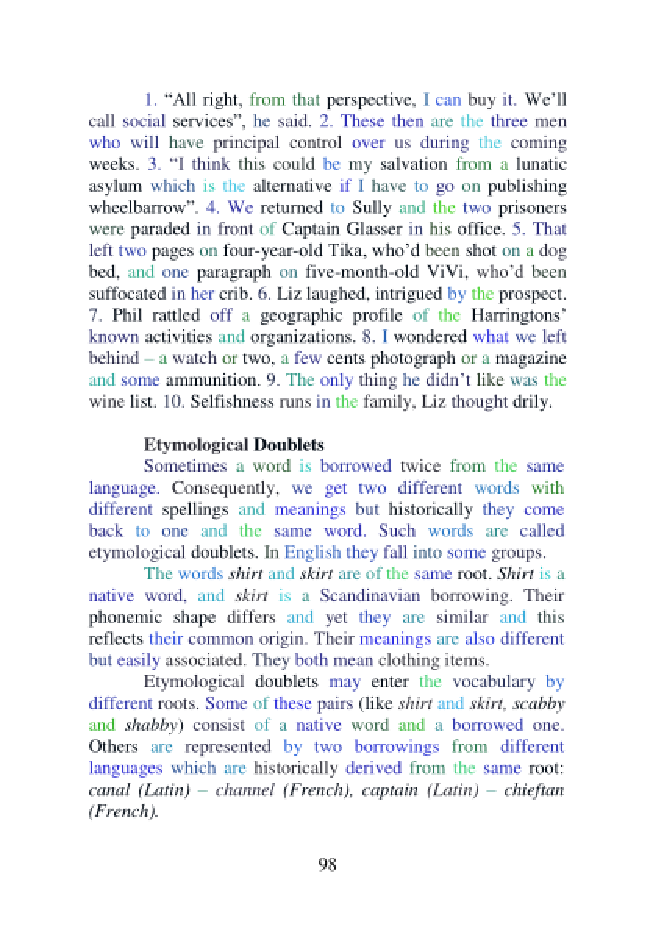
\includegraphics[width=\textwidth]{images/chapter4/plain.pdf}
        \caption{Plain}
      \end{subfigure}
      \begin{subfigure}[b]{0.24\textwidth}
        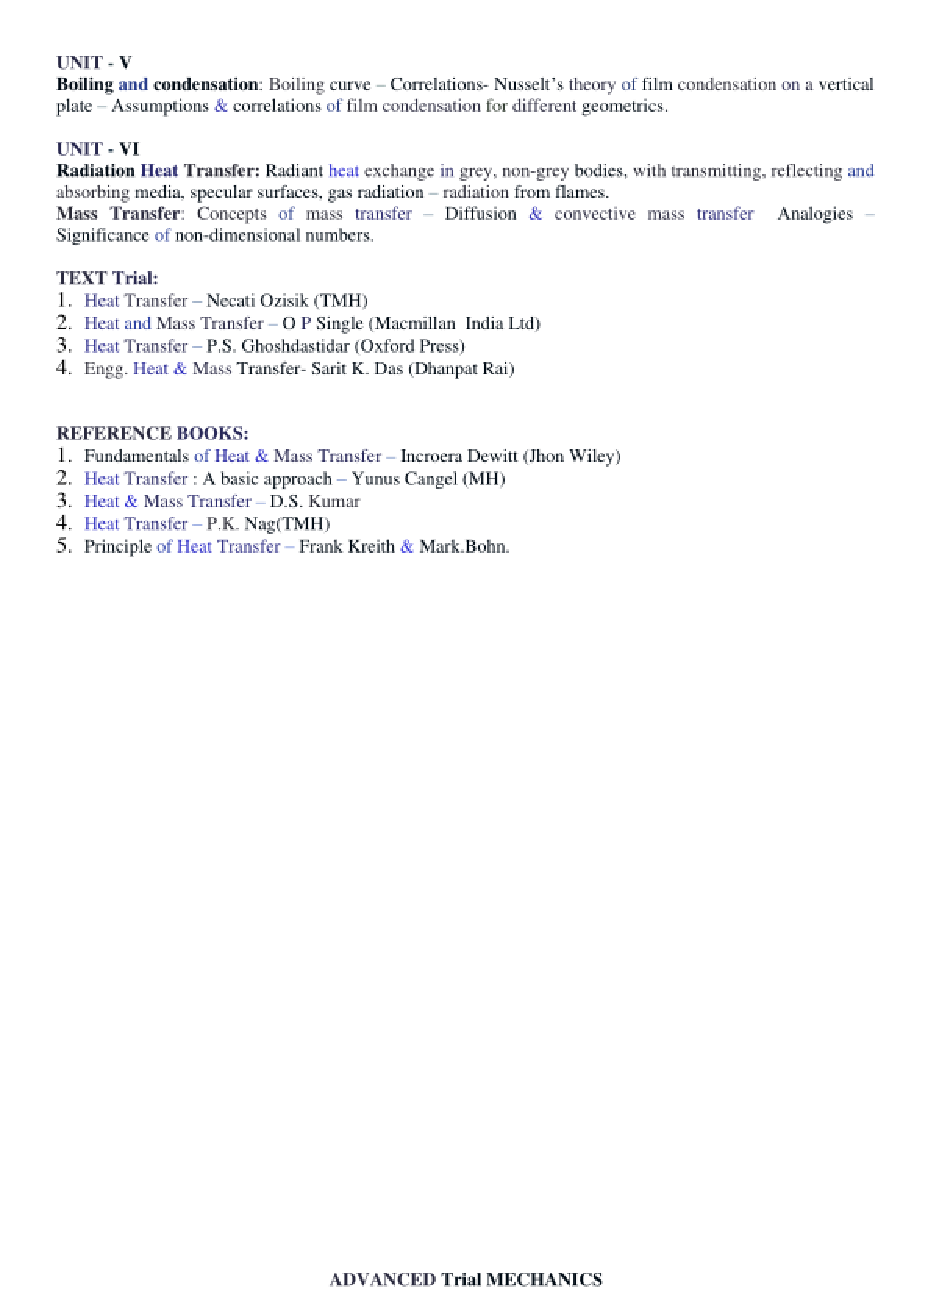
\includegraphics[width=\textwidth]{images/chapter4/list.pdf}
        \caption{List}
      \end{subfigure}
      \begin{subfigure}[b]{0.24\textwidth}
        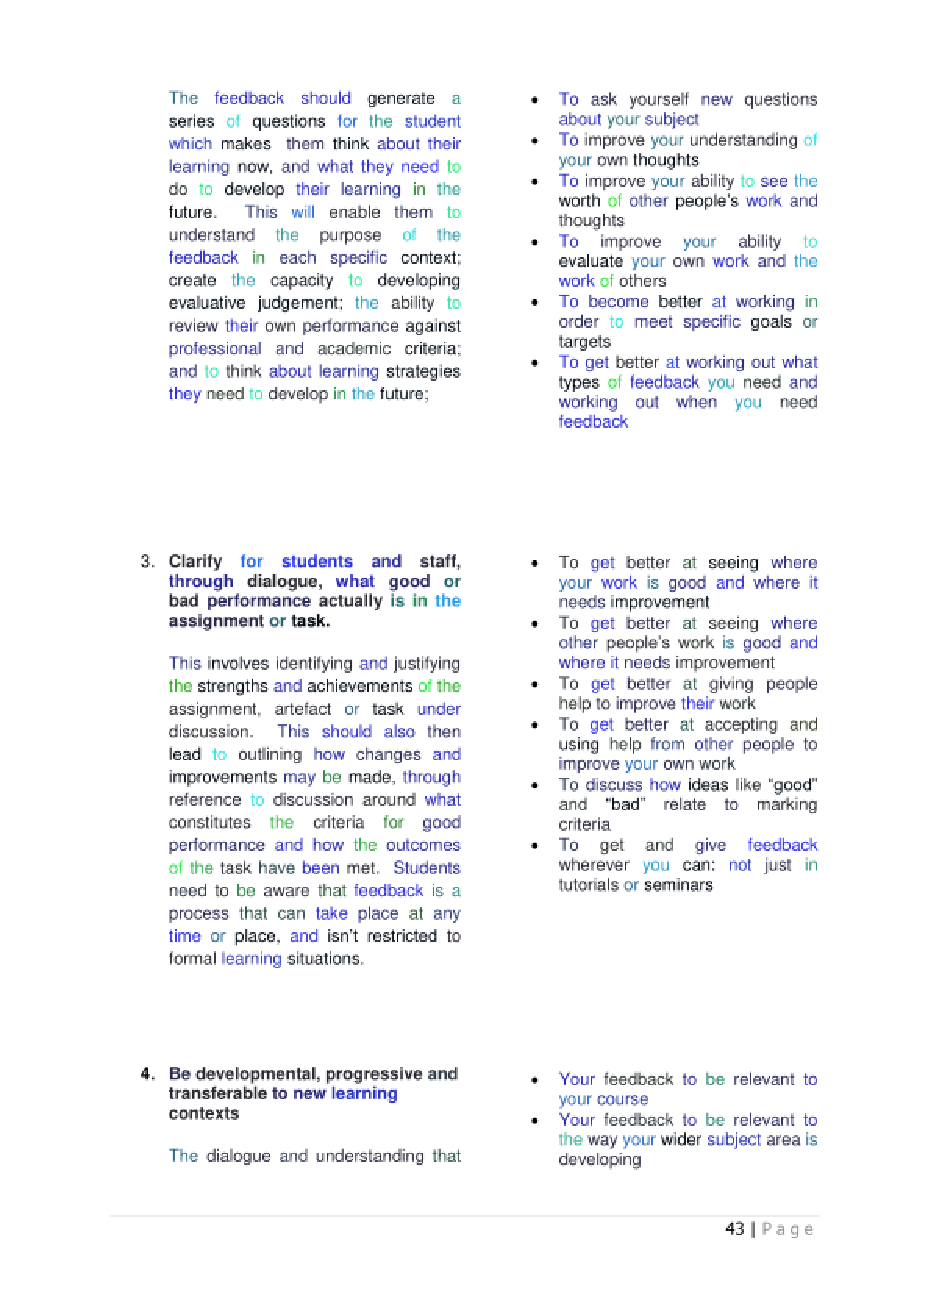
\includegraphics[width=\textwidth]{images/chapter4/multicolumn.pdf}
        \caption{Multicolumn}
      \end{subfigure}
      \begin{subfigure}[b]{0.24\textwidth}
        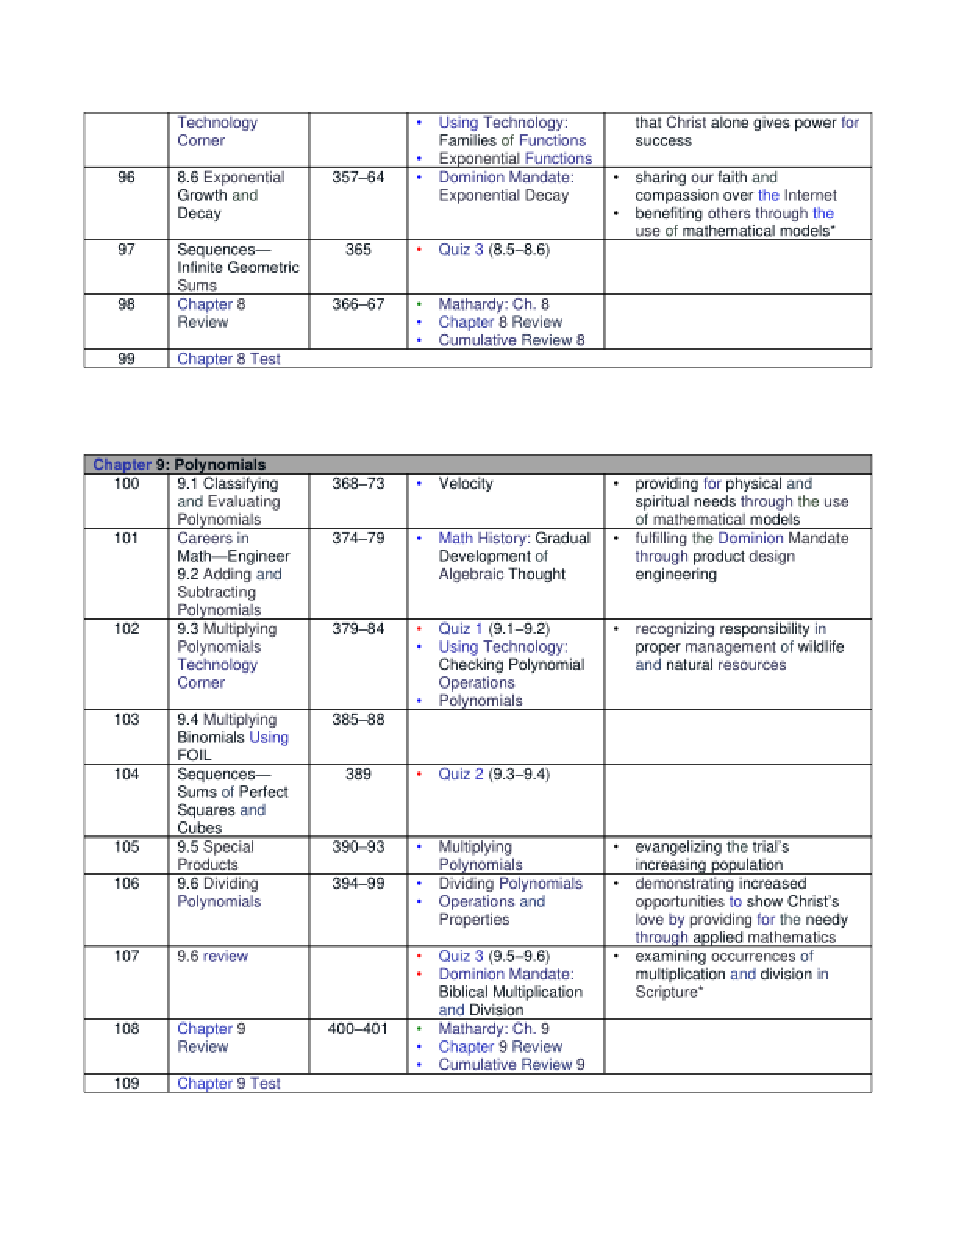
\includegraphics[width=\textwidth]{images/chapter4/tables.pdf}
        \caption{Table}
      \end{subfigure}
    \caption{Examples of documents for each layout category, arranged from the simplest to the most complex.}
    \label{fig:layout-examples}
\end{figure}

\begin{table}
  \centering
  \small
  \begin{adjustbox}{max width=\textwidth}
  \begin{threeparttable}
  \begin{tabular}{lcccccccc}
      \toprule
          & & \multicolumn{4}{c}{\textbf{Layout Type}} & \\
          & & \textbf{Plain} & \textbf{Lists} & \textbf{Multicolumn} & \textbf{Tables}\\
      \midrule
      Tesseract OCR \citep{kay2007tesseract} & & 78.71 & 72.75 & 61.43 & 36.97 \\
      DocTR \citep{doctr2021} & & 86.83 & 77.83 & 82.54 & 66.11 \\
  \bottomrule
  \end{tabular}
  \end{threeparttable}
  \end{adjustbox}
  \caption{Accuracy (in \%) obtained by each \ac{OCR} engine, for each document layout type.}
  \label{table:ocr-preliminary-experiments}
\end{table}

\begin{figure}
    \centering
    \small
      \begin{subfigure}[b]{\textwidth}
        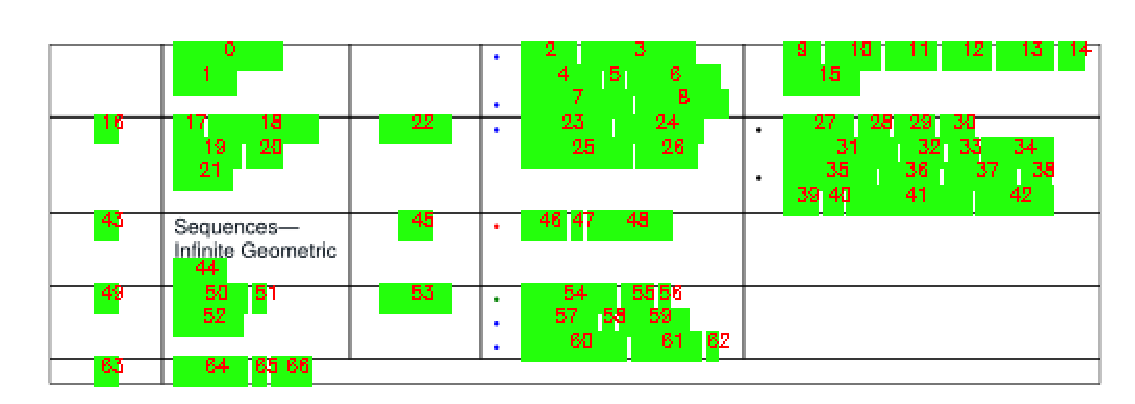
\includegraphics[width=\textwidth]{images/chapter4/gold_tables.pdf}
        \caption{Ground-truth reading order}
      \end{subfigure}
      \begin{subfigure}[b]{\textwidth}
        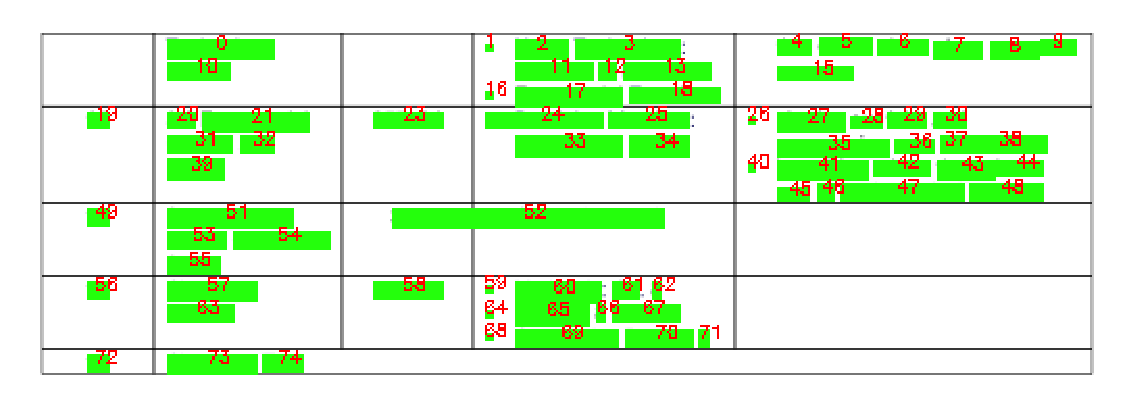
\includegraphics[width=\textwidth]{images/chapter4/tesseract_tables.pdf}
        \caption{Reading order obtained through Tesseract}
      \end{subfigure}
    \caption{Ground-truth reading order (a) compared to the reading order generated by Tesseract (b) for a sample table. Non-highlighted text indicates that it does not appear in the serialized sequence.}
    \label{fig:reading-orders-table}
\end{figure}

\begin{figure}
  \centering
  \small
      \begin{subfigure}[b]{0.5\textwidth}
        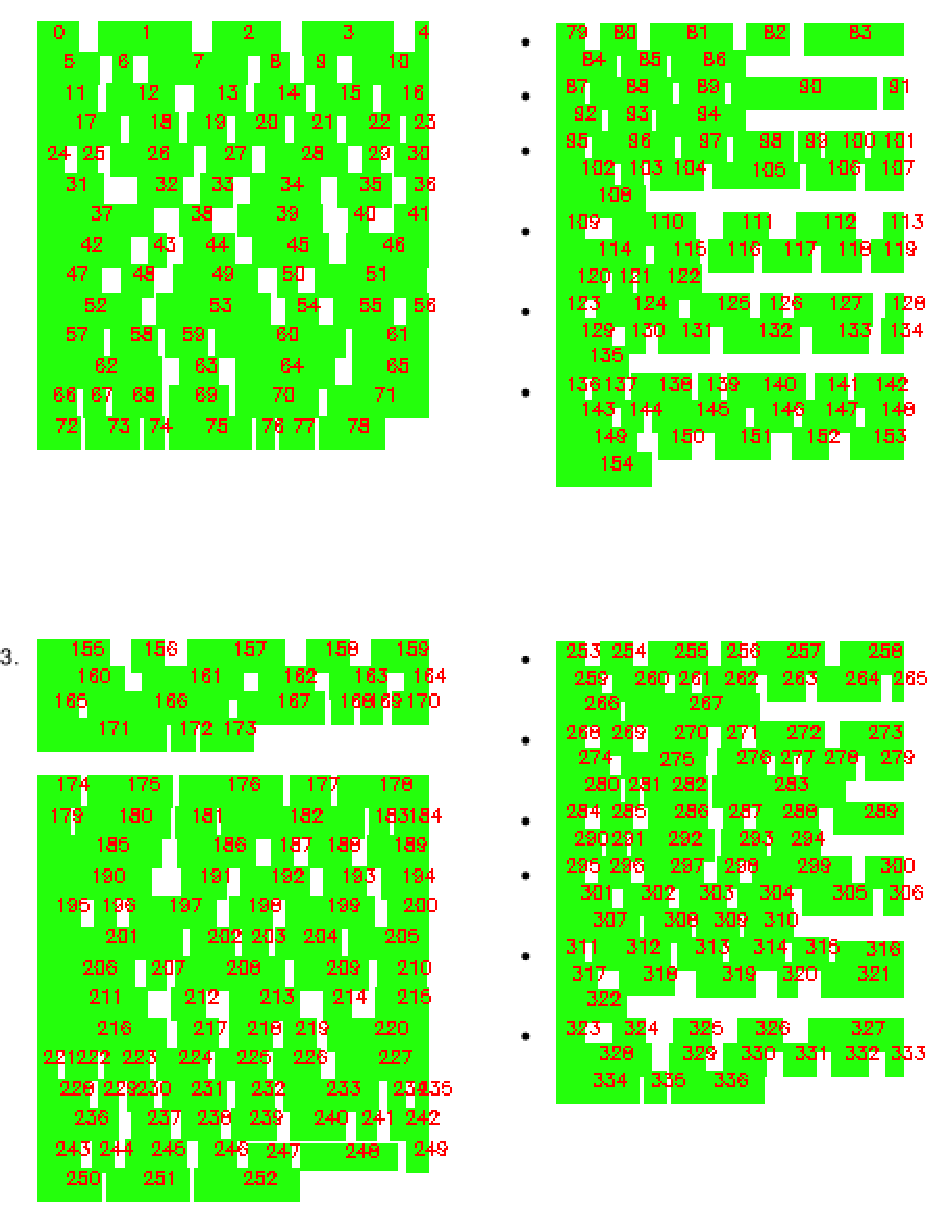
\includegraphics[width=\textwidth]{images/chapter4/gold_multicolumn.pdf}
        \caption{Ground-truth}
      \end{subfigure}
      \begin{subfigure}[b]{0.5\textwidth}
        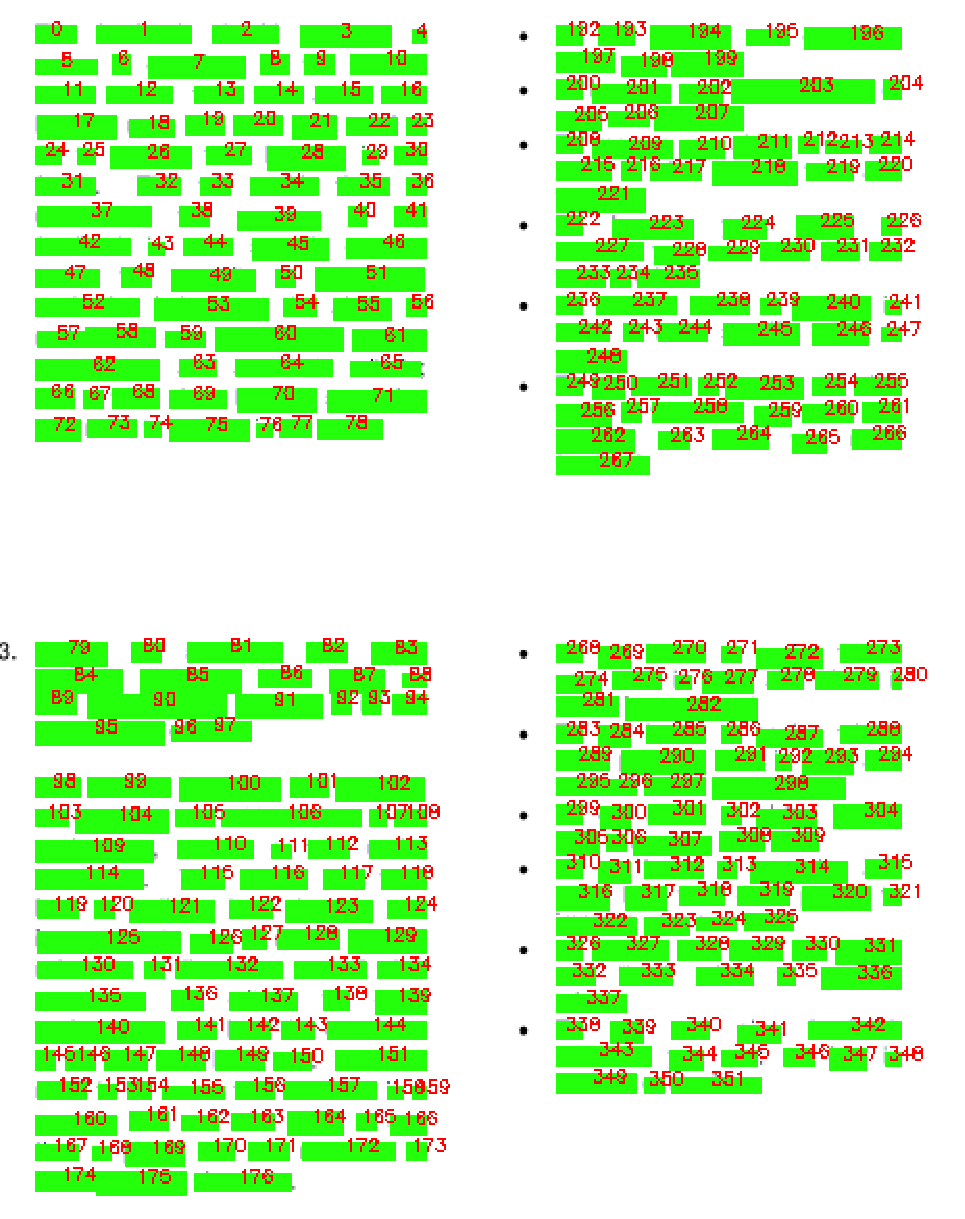
\includegraphics[width=\textwidth]{images/chapter4/tesseract_multicolumn.pdf}
        \caption{Tesseract}
      \end{subfigure}
    \caption{Ground-truth reading order (a) compared to the reading order generated by Tesseract (b) for a document with a two-column layout. The document was cropped for better visibility. Non-highlighted text indicates that it does not appear in the serialized sequence.}
    \label{fig:reading-orders-multicolumn}
\end{figure}


\subsection{Layout2Pos Module}

Building on the insights gained from the previous experiment, accurately retrieving the correct reading order poses a significant challenge for \ac{OCR} engines. We argue that it is possible to retrieve the correct reading order by leveraging the document layout. To address this, we propose a novel approach, \textit{Layout2Pos}, a transformer-based module that discards the reading order generated by \ac{OCR} and, instead, learns 1D position embeddings exclusively from the spatial positions of tokens. Layout2Pos is a stack of Transformer layers designed to generate a corresponding sequence of 1D position embeddings based on spatial information. In the following, we elaborate on the process of encoding spatial information into layout embeddings, followed by an in-depth description of our Layout2Pos module.

\subsubsection{Encoding Layout Information}

The spatial position of a token is represented by its bounding box in the document page image, denoted as $(x_0, y_0, x_1, y_1)$, where $(x_0, y_0)$ and $(x_1, y_1)$ correspond to the coordinates of the top-left and bottom-right corners, respectively. We discretize and normalize these coordinates to integers within the range of $[0, ..., 1000]$. Four embedding tables are employed to encode spatial positions: two for the coordinate axes ($x$ and $y$), and the other two for the bounding box size (width and height). In line with LayoutLMv2 \citep{xu2020layoutlmv2}, the final layout embedding $\bell \in \mathbb{R}^{d_{\ell}}$ of a token positioned at $(x_0, y_0, x_1, y_1)$ is defined as follows:

\begin{equation}
\begin{split}
    \bell & = \text{LayoutEmb}_x(x_0) \mathbin\Vert \text{LayoutEmb}_y(y_0) \\
    & \mathbin\Vert \text{LayoutEmb}_x(x_1) \mathbin\Vert \text{LayoutEmb}_y(y_1) \\
    & \mathbin\Vert \text{LayoutEmb}_w(x_1 - x_0) \mathbin\Vert \text{LayoutEmb}_h(y_1 - y_0), 
\end{split}
\label{eq:layout-embeddings}
\end{equation}

\noindent where $\mathbin\Vert$ denotes concatenation.

Following LayoutLMv2, we also encode spatial relative positions as bias terms added to the attention scores to explicitly capture the spatial relationship between tokens. For each pair of bounding boxes $((x_0, y_0, x_1, y_1), (x^{\prime}_0, y^{\prime}_0, x^{\prime}_1, y^{\prime}_1))$, we compute the horizontal distance $x^{\prime}_0 - x_0$ between the left edge of each box and the vertical distance $y^{\prime}_1 - y_1$ between the bottom edge of each box. To provide additional insights into the spatial relationships of tokens, we also compute the horizontal distance $x^{\prime}_1 - x_0$ between the right edge of one box and the left edge of the other (indicating information about the combined length). Furthermore, we calculate the horizontal distance $x^{\prime}_1 - x_1$ between the right edge of each box, providing information about the length of the second token in the pair. In addition, we consider \textit{line} and \textit{column} relative positions. Understanding the relative positions within lines helps the sequential structure of the document, aiding in distinguishing between different parts of the document. On the other hand, the relative positions within columns is valuable for documents with multicolumn layouts, offering insights into the spatial arrangement of text across columns. Overall, line and column information enhance the model's ability to capture the structural organization of textual content within documents. Hence, for each bounding box, we identify other bounding boxes that share the same line/column. This is determined by whether the horizontal/vertical line passing through the center of the box intersects with the other bounding boxes. If there is an intersection, the boxes are considered to be on the same line/column. For each token, we determine its positions within its corresponding line and column. Then, we compute the relative sequential distance $\delta^{line}_{ij}$ and $\delta^{column}_{ij}$ between elements within each line and column. If they do not belong to the same line or column, the distance is set to 1000. 

Formally, let $\bm{q}^{\ell}_i$ and $\bm{k}^{\ell}_i$ denote the query and key projections obtained from the layout embedding $\bell_i$ of token $i$. In Layout2Pos, attention is re-defined as:

\begin{equation}
  \begin{split}
  \alpha_{ij} &= \dfrac{1}{\sqrt{d}} \left(\bm{q}^{\ell}_i \cdot \bm{k}^{\ell}_j\right) \\
              & + b^{(2D_x)}_{x^{(j)}_{0} - x^{(i)}_{0}} + b^{(2D_y)}_{y^{(j)}_{1} - y^{(i)}_{1}} + b^{(2D_x)}_{x^{(j)}_{1} - x^{(i)}_{0}} + b^{(2D_x)}_{x^{(j)}_{1} - x^{(i)}_{1}} \\
              & + b^{(l)}_{\delta^{l}_{ij}}  + b^{(c)}_{\delta^{c}_{ij}},
  \end{split}
  \label{eq:layout2pos-attention}
\end{equation}

\noindent where $\bm{b}^{(2D_x)}$, $\bm{b}^{(2D_y)}$, $\bm{b}^{(l)}$, and $\bm{b}^{(c)}$correspond to the horizontal, vertical, line, and column relative position biases, respectively. The biases are different among attention heads but shared across all layers. The relative sequential distances between elements within lines and columns, $\bm{\delta}^{(line)}$ and $\bm{\delta}^{(column)}$, are defined as follows:

\begin{equation}
  \begin{split}
    \delta^{l}_{ij} &= 
        \begin{cases}
          posInLine(j) - posInLine(i), & \text{if } line(j) = line(i)\\
            1000,              & \text{otherwise}.
        \end{cases} \\
    \delta^{c}_{ij} &= 
      \begin{cases}
        posInColumn(j) - posInColumn(i), & \text{if } column(j) = column(i)\\
          1000,              & \text{otherwise}.
      \end{cases}
  \end{split}
\end{equation}

\subsubsection{Learning 1D Position Embeddings from Layout Information}

\begin{figure}
  \centering
  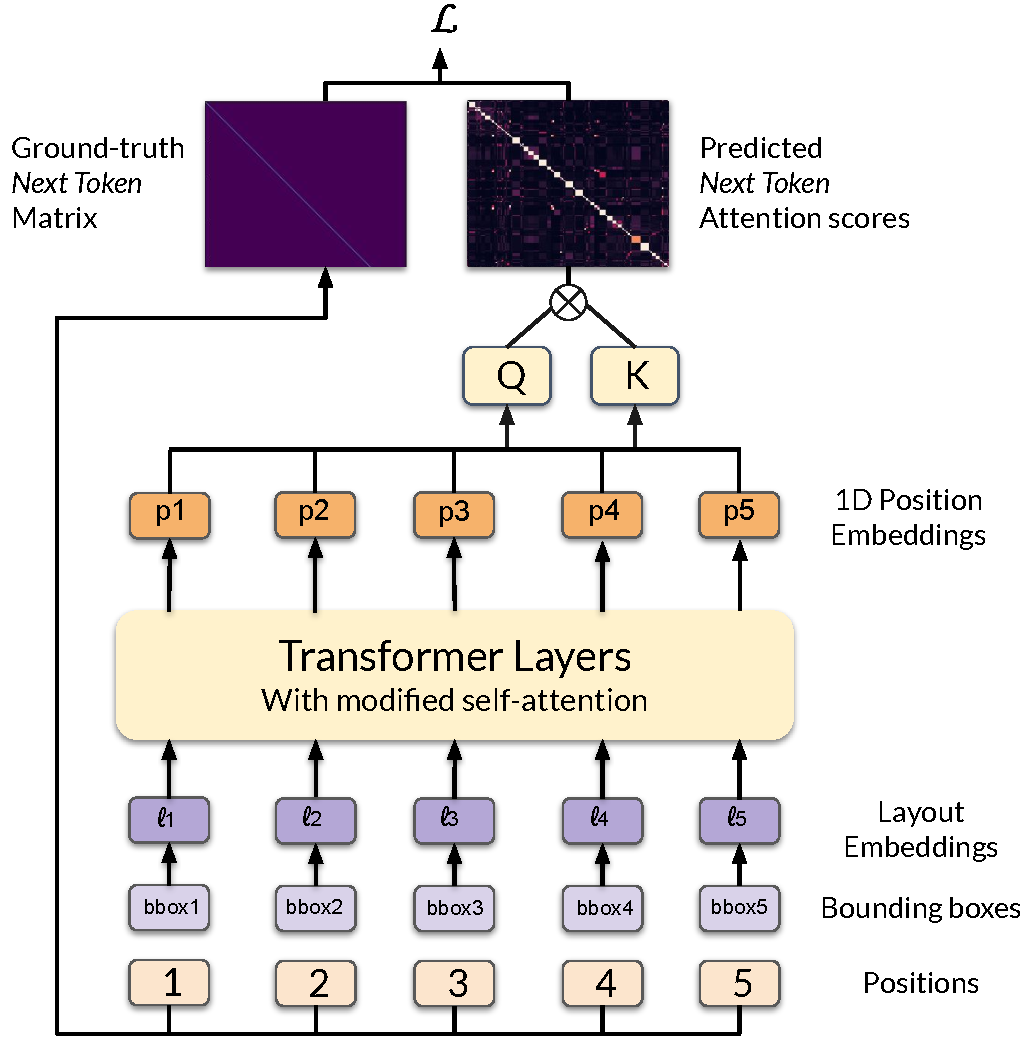
\includegraphics[width=0.75\textwidth]{images/chapter4/Layout2Pos.pdf}
  \caption{Layout2Pos Architecture. The input consists of a sequence of token bounding box coordinates, transformed into corresponding embedding sequences. Self-attention in the stack of Transformer layers is modified as defined by Equation~\ref{eq:layout2pos-attention}. $\bm{Q}$ and $\bm{K}$ are the queries and keys obtained by projecting the 1D position embeddings. The attention scores obtained through dot-product are compared against the ground-truth matrix to compute the Next Token Prediction loss.}
  \label{fig:layout2pos-module}
\end{figure}

Given a sequence of layout embeddings as defined by Equation~\ref{eq:layout-embeddings}, Layout2Pos employs a stack of $M$ Transformer layers to contextualize the sequence. The outputs of the last layer serve as 1D position embeddings:

\begin{equation}
  \bm{p}_i = \bm{h}^M(\bell_i).
\end{equation}

\noindent Then, these 1D position embeddings are used to compute the attention matrix $\bm{A}$, \textit{i.e.}, alignment scores between every token:

\begin{equation}
  A_{ij} = \left(\bm{p}_i \bm{W}^q\right)\left(\bm{p}_j \bm{W}^k\right).
\end{equation}

\noindent We assume that the attention matrix $\bm{A}$ carries information about the reading order, \textit{i.e.}, $A_{ij}$ represents the probability that the $j$-th token follows the $i$-th token. Let $N$ denote the ground-truth binary matrix obtained from the ground-truth reading order, where $N_{ij}$ equals $1$ if token at position $j$ is the \textit{next} token after token at position $i$ in the sequence, and $0$ otherwise. We define the \textit{Next Token Prediction} strategy, which consists in using the attention matrix $\bm{A}$ to predict the next token of each token in the sequence (\textit{next token matrix}). The corresponding loss is defined as follows:

\begin{equation}
  \mathcal{L}_{NTP} = - \sum_{i=1}^n \sum_{j=1}^n N_{ij} \log\left(\textrm{softmax}(A_{ij})\right).
\end{equation}

\noindent As such, Layout2Pos is trained to capture the relationship between spatial arrangement of tokens and reading order. This is done by ensuring that the attention matrix $\bm{A}$ derived from the computed 1D position embeddings carries information about the next token for each token in the sequence. The architecture of Layout2Pos is depicted in Figure~\ref{fig:layout2pos-module}. It is noteworthy that a global reading order is unnecessary; there is no requirement to establish an order between two words that belong to segments that have no relation to each other.

% Given that each token is treated as a bounding box defined by its size and position, a significantly smaller representation space can be chosen for layout features compared to text. As Layout2Pos does not need to understand semantic content, it may require a smaller latent space dimension than conventional multimodal pre-trained models. 

\subsubsection{Integrating Layout2Pos into a Sequence-to-Sequence Framework}

\begin{figure}
  \centering
  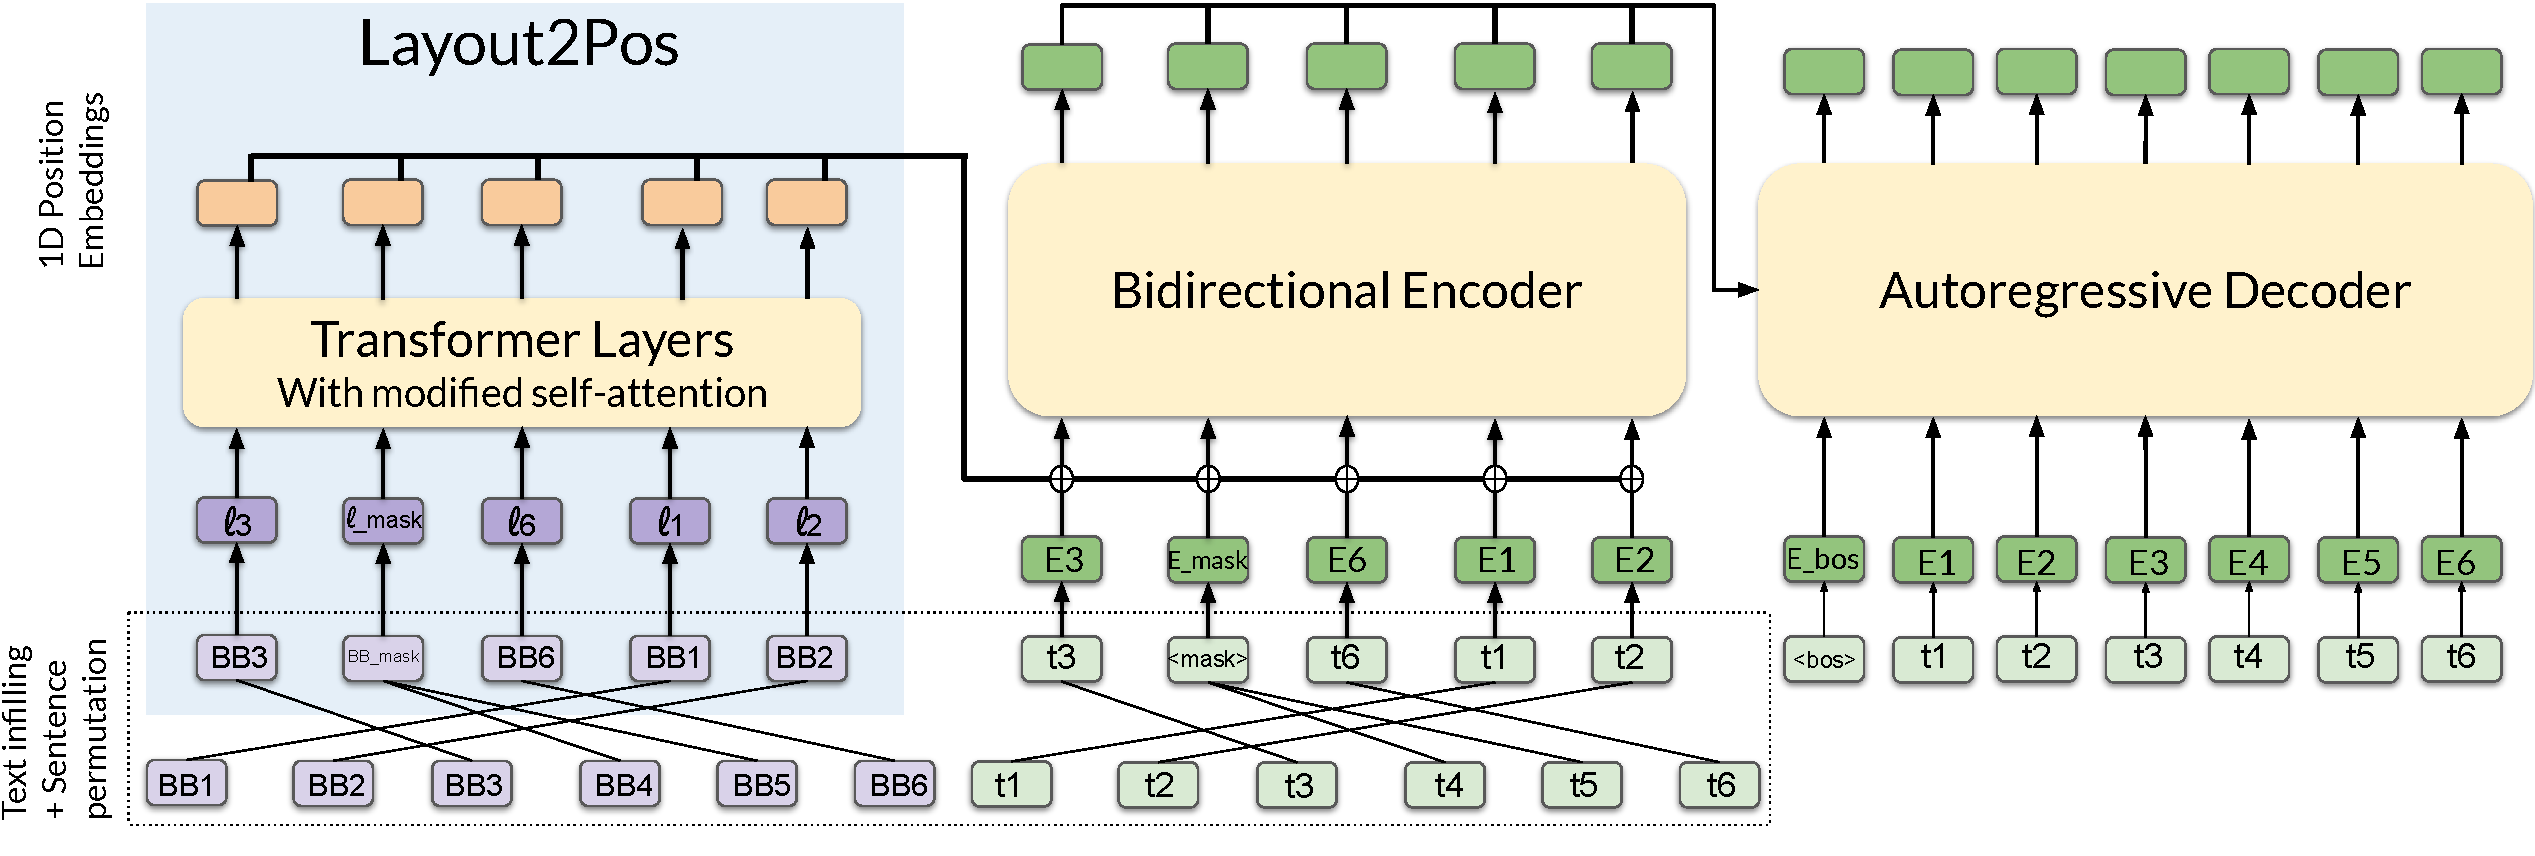
\includegraphics[width=\textwidth]{images/chapter4/Layout2Pos+BART.pdf}
  \caption{Architecture of Layout2Pos integrated into a BART model, \textit{i.e.}, BART+Layout2Pos. The input consists of two components: a sequence of tokens and a sequence of token bounding box coordinates. The sequence of tokens is corrupted using \textit{text infilling and sentence permutation}, and the sequence of token bounding boxes is altered accordingly. Both  sequences are transformed into corresponding embedding sequences. Layout2Pos learns to calculate 1D position embeddings from layout embeddings using the \textit{next token prediction} loss. The sequence of 1D position embeddings are subsequently added to the token embeddings. The resulting embeddings are fed into an encoder-decoder model, trained to reconstruct the original sequence of tokens (\textit{denoising}).}
  \label{fig:layout2pos-ed}
\end{figure}

Layout2Pos can be integrated into any language model, removing the reliance on sequential position information. This is achieved by substituting the traditional 1D position encodings derived from \ac{OCR} by the 1D position embeddings produced by Layout2Pos. Specifically, we integrate Layout2Pos into a Transformer encoder-decoder architecture, as illustrated in Figure~\ref{fig:layout2pos-ed}. The model receives a sequence of tokens and the corresponding sequence of token bounding boxes as input, both embedded using embedding tables. The sequence of position embeddings, obtained by Layout2Pos, is added to the sequence of token embeddings, and the resulting sequence is input to the bidirectional encoder. The output sequence of contextualized embeddings is fed to the autoregressive decoder to generate the target sequence.

\paragraph{Training} Layout2Pos is simultaneously trained with the encoder-decoder model. While the module learns to predict the subsequent token of each token based on layout information, the encoder-decoder follows a pre-training approach similar to \ac{BART}  \citep{lewis2006building}. The model is trained to reconstruct the original input sequence from a corrupted version (\textit{denoising}). Sequences are corrupted by randomly replacing text spans with a single mask token (\textit{text inflling}) and permuting sentences (\textit{sequence permutation}). The corrupted sequence is encoded using the bidirectional encoder, and the autoregressive decoder is trained to reconstruct the original sequence. We refer to the overall model as BART+Layout2Pos.

\paragraph{Inference} To determine how the model predicts the next token of the sequence, BART+Layout2Pos employs a customized variant of beam search to generate tokens while minimizing repetitions. In this modified version, the generated tokens, if already present in the source sequence, are constrained not to occur more frequently than in the original source. This constraint is enforced by keeping count of the number of occurrences of each token in the source sequence within the target sequence and masking the corresponding logit when the maximum occurrence is reached. This approach aims to enhance the coherence of the generated sequences by ensuring that the generated tokens align appropriately with the content of the input document, minimizing redundancy and improving overall output quality.


\section{Experiments and Results}

In this section, we provide an overview of the datasets used for pre-training our models and conducting visual information extraction tasks. Furthermore, we provide details on the experimental setup, covering baselines, pre-training methodologies, and fine-tuning protocols. We evaluate our models on the Next Token Prediction task, along with three benchmark visual information extraction tasks. 

\subsection{Data}

\subsubsection{Pre-training Data}

Following a common practice in the field of Document Understanding, we collect data from the IIT-CDIP collection \citep{lewis2006building} to build our pre-training dataset. IIT-CDIP consists of around 11 million document page images of various types and layouts, including news articles, scientific reports, handwritten materials, and more. The collection contains scanned images of documents, introducing challenges related to image quality, resolution, and potential artifacts. As such, we leverage IIT-CDIP to pre-train models under realistic conditions. We select over 7 million document images from the collection to build our pre-training dataset. To extract text and bounding boxes from the documents, we use DocTR \citep{doctr2021}. Due to potential serialization errors induced by DocTR, and given that the Next Token Prediction task requires documents with proper reading orders, IIT-CDIP is only used for training models in language modeling tasks. 

To enable Layout2Pos to effectively learn the correct reading order of documents, we use the 500k documents from the ReadingBank dataset \citep{wang2021layoutreader}. These documents are serialized and annotated with high-quality reading order annotations, serving as the training data for both Next Token Prediction and language modeling tasks. Our final pre-training corpus is referred to as IIT-CDIP+ReadingBank. 

In cases where a word is split into multiple tokens, earlier approaches based on word-level bounding boxes typically assign the word's bounding box to all the tokens within that word. However, this approach is inefficient for next token prediction, given that tokens within the same word would share identical layout embeddings, hence hindering accurate predictions of the next token. Therefore, we approximate token-level bounding boxes by dividing each word-level bounding box by the number of characters in the word.

\subsubsection{Data for Visual Information Extraction}

We evaluate our approach on visual information extraction tasks, where the goal is to extract semantic entities from visually-rich documents, based on a set of pre-defined keys. This evaluation is conducted using three benchmark for visual information extraction, each covering different document types: FUNSD \citep{jaume2019funsd}, CORD \citep{park2019cord}, and SROIE \citep{huang2019icdar2019}. For each dataset, we use the reading order provided. To maintain consistency with pre-training data, we employ approximated token-level bounding boxes.

\paragraph{FUNSD} \citep{jaume2019funsd} is a form understanding dataset consisting of 199 real, noisy and scanned forms where each sample contains key-value pairs of form entities. There are three keys for which values have to be extracted: \textit{question}, \textit{answer}, and \textit{header}. The dataset is split into 149 samples for training and 50 for test.

\paragraph{CORD (v1)} \citep{park2019cord} is a receipt understanding dataset containing 1,000 scanned Indonesian receipts with 30 keys categorized into four superclasses: \textit{menu}, \textit{subtotal}, \textit{total}, and \textit{void}. We exclude keys with very few occurrences,\footnote{Discarded keys are: menu.etc, menu.itemsubtotal, menu.sub\_etc, menu.sub\_unitprice, menu.vatyn, void\_menu.nm, void\_menu.price, sub\_total.othersvc\_price.} which results in 22 keys grouped into three superclasses. The dataset is divided into 800 examples for training, 100 for validation, and 100 for test.

\paragraph{SROIE} \citep{huang2019icdar2019} is another receipt understanding dataset comprising 973 scanned receipts written in English. The task involves extracting entities for four keys: \textit{total}, \textit{date}, \textit{company}, and \textit{address}. The dataset is partitioned into 626 samples for training and 347 for test. 

\subsection{Experimental Settings}

Models were implemented in Python using PyTorch \citep{paszke2017automatic} and Hugging Face \citep{wolf2019huggingface} librairies. 

\subsubsection{Baselines}

We compare our approach with BART+2D, a layout-augmented \ac{BART} model which relies on 1D position embeddings derived from \ac{OCR}-induced positions. These 1D position embeddings are calculated using embedding tables and are subsequently added to textual features. Layout embeddings, computed from bounding boxes using Equation~\ref{eq:layout-embeddings}, are incorporated to the resulting embeddings to construct the input embeddings. Following LayoutLMv2 \citep{xu2020layoutlmv2}, self-attention is modified as follows: 

\begin{equation}
  \alpha_{i,j} = \dfrac{1}{\sqrt{d}} \bm{q}_i \cdot \bm{k}_j + b^{(1D)}_{j - i} + b^{(2D_x)}_{x^{(j)}_{0} - x^{(i)}_{0}} + b^{(2D_y)}_{y^{(j)}_{1} - y^{(i)}_{1}},
\end{equation}

\noindent where $\bm{b}^{(1D)}$, $\bm{b}^{(2D_x)}$, and $\bm{b}^{(2D_y)}$ denote the sequential, horizontal, and vertical relative position biases, respectively. BART+2D follows the same training and inference procedures as BART+Layout2Pos.

Additionally, we report the performance of two layout-aware encoder-only models. We use LayoutLM and a variant of LayoutLMv2 that discards visual information (referred to as LayoutLMv2-no-visual), ensuring a fair comparison with our approach. 

\subsubsection{Pre-training}

\paragraph{Encoder-decoder Models} Layout2Pos is composed of 2 layers with 12 attention heads and a hidden size of 768. The final attention calculation, responsible for computing the next token matrix, involves a single attention head. Following the \ac{BART} base model, both the encoder and decoder in BART+Layout2Pos and BART+2D are comprised of 6 layers, each with 12 attention heads and a representation space dimensionality of 768. BART+Layout2Pos encompasses a total of 156 million parameters, while BART+2D amounts to 140k parameters. 

Both models are trained from scratch on IIT-CDIP+ReadingBank. The documents are tokenized 
using the tokenizer of the base variant of \ac{BART} (bart-base) shared through the Hugging Face Model Hub. The training spans 10 epochs, amounting to 500k optimization steps, including 59k for warmup. For each model, we select the checkpoint with the best validation loss. We use a maximum sequence length of 512, a batch size of 80, and a learning rate of 1e-4. For text infilling, we set the masking ratio to 0.3, with span lengths drawn from a Poisson distribution where $\lambda$ equals 3. Every sentence is permuted. Experiments were ran on Nvidia Titan RTX with 25GB. 

\paragraph{Encoder-only baselines} For LayoutLM, the microsoft/layoutlm-base-uncased checkpoint with 113M parameters is used. Following the base architecture of LayoutLMv2, LayoutLMv2-no-visual is composed of a 12-layer Transformer encoder with 12 attention heads and a hidden size of 768, amounting to 110M parameters. The model is also pre-trained from scratch, using \ac{MVLM} on IIT-CDIP+ReadingBank. The documents are tokenized using the tokenizer of microsoft/layoutlm-base-uncased. The pre-training extends over 10 epochs, with a maximum sequence length of 512, a batch size of 80, and a learning rate of 1e-4.


\subsubsection{Visual Information Extraction}

\paragraph{Sequence-labeling approaches}

To compare our sequence-to-sequence approach with the traditional sequence labeling method on visual information extraction tasks, we employ LayoutLM and LayoutLMv2-no-visual. For every dataset, the maximum sequence length is set to 512. Both models are fine-tuned for 100 on FUNSD, and 20 epochs on SROIE and CORD. The learning rate is set to 5e-5 for all models and datasets.

\paragraph{Sequence-to-sequence models} We frame visual information extraction as a sequence-to-sequence problem, wherein the document serves as the input, and the output consists of a series of extracted entities paired with their corresponding keys. In Figure~\ref{fig:source-target-sample}, we provide an example of a source document from SROIE and its corresponding target sequence. In the case of the CORD dataset, which features numerous keys that may not necessarily appear in every document, we augment the target sequences by including keys not found in the corresponding documents and assigning their values to "N/A". 

Entities and their corresponding keys are extracted from both the generated sequences and the ground-truth sequences. The pairs of generated and ground-truth \textit{(key, entities)} are then compared to compute precision, recall, and F1 score. If an entity is correctly tagged and appears the same number of times or less than in the input but occurs more frequently than in the target sequence, we ignore the excess occurrences. To provide further insights into the model's errors, additional metrics are defined. The \textit{hallucination rate} represents the percentage of entities generated by the model that do not match with any text in the input sequence. It is used to measure how often the model produces content that is not grounded in the input. The \textit{wrong label rate} represents the proportion of generated entities present in the ground-truth but mislabeled by the model. It measures how often the model generates the right entities but mislabels them. The \textit{omission rate} denotes the proportion of ground-truth entities that were not generated by the model, providing insights into how often the model omits entities. Lastly, the \textit{"Other" rate} is the percentage of generated entities that, in the ground-truth, correspond to the category "Other". This metric assesses the frequency with which the model categorizes a text as an entity when it is not.

% The \textit{repetition rate} is the percentage of entities that are part of the ground-truth entities but are repeated excessively. It quantifies the frequency with which the model generates duplicated entities. 

% We attribute the improvement to the fact that, although the advanced serialization is not used for fine-tuning datasets, the model has the ability to understand the proper reading order of documents after pre-training.

For all three datasets, we set the maximum source sequence length to 512. Documents that exceed this length are split into sequences, each consisting of 512 tokens. For each input sequence, we formulate a target sequence containing the pairs of values-keys contained in the input sequence. In the case of FUNSD, we truncate target sequences at 512 tokens. As for SROIE and CORD, the maximum target sequence length is set to 64 and 384 tokens, respectively. Models are fine-tuned for 100 epochs on FUNSD and 10 on CORD. As for SROIE, fine-tuning is conducted for 40 epochs for BART+2D and 100 epochs for BART+Layout2Pos. The learning rate is set to 5e-5 for all models and datasets. During inference, we set the number of beams to 5.

Considering that the pre-training phase has allowed BART+Layout2Pos to understand the correct reading order of documents, and acknowledging the potential discrepancies in the reading order within visual information extraction datasets, we opt not to use the Next Token Prediction strategy during fine-tuning.

% \begin{figure}
%   \centering
%   \small
%       \begin{subfigure}[b]{0.3\textwidth}
%         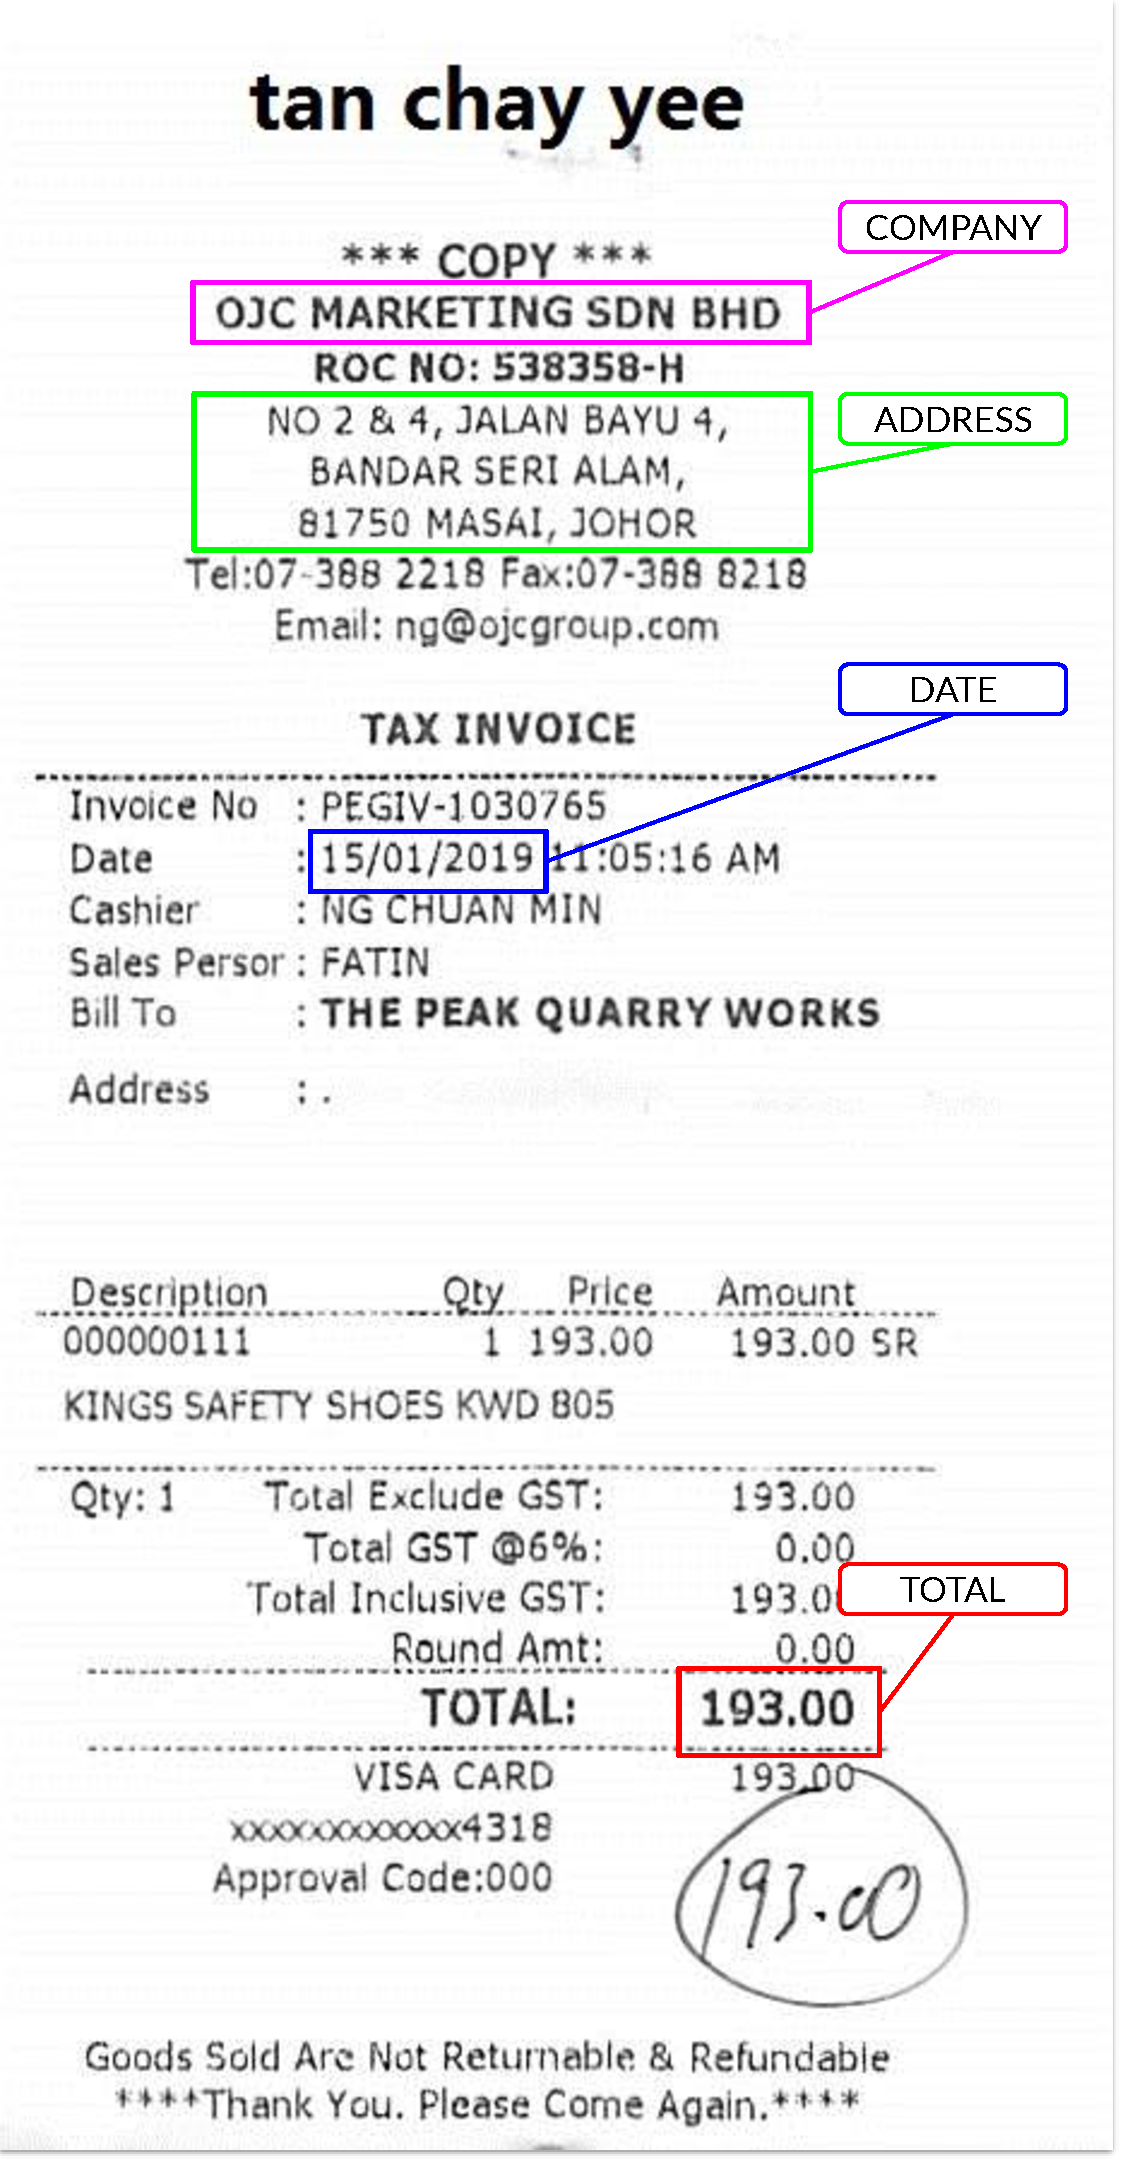
\includegraphics[width=\textwidth]{images/chapter4/sroie_sample.pdf}
%         \caption{Source document}
%       \end{subfigure}
%       \begin{subfigure}[b]{0.25\textwidth}
%         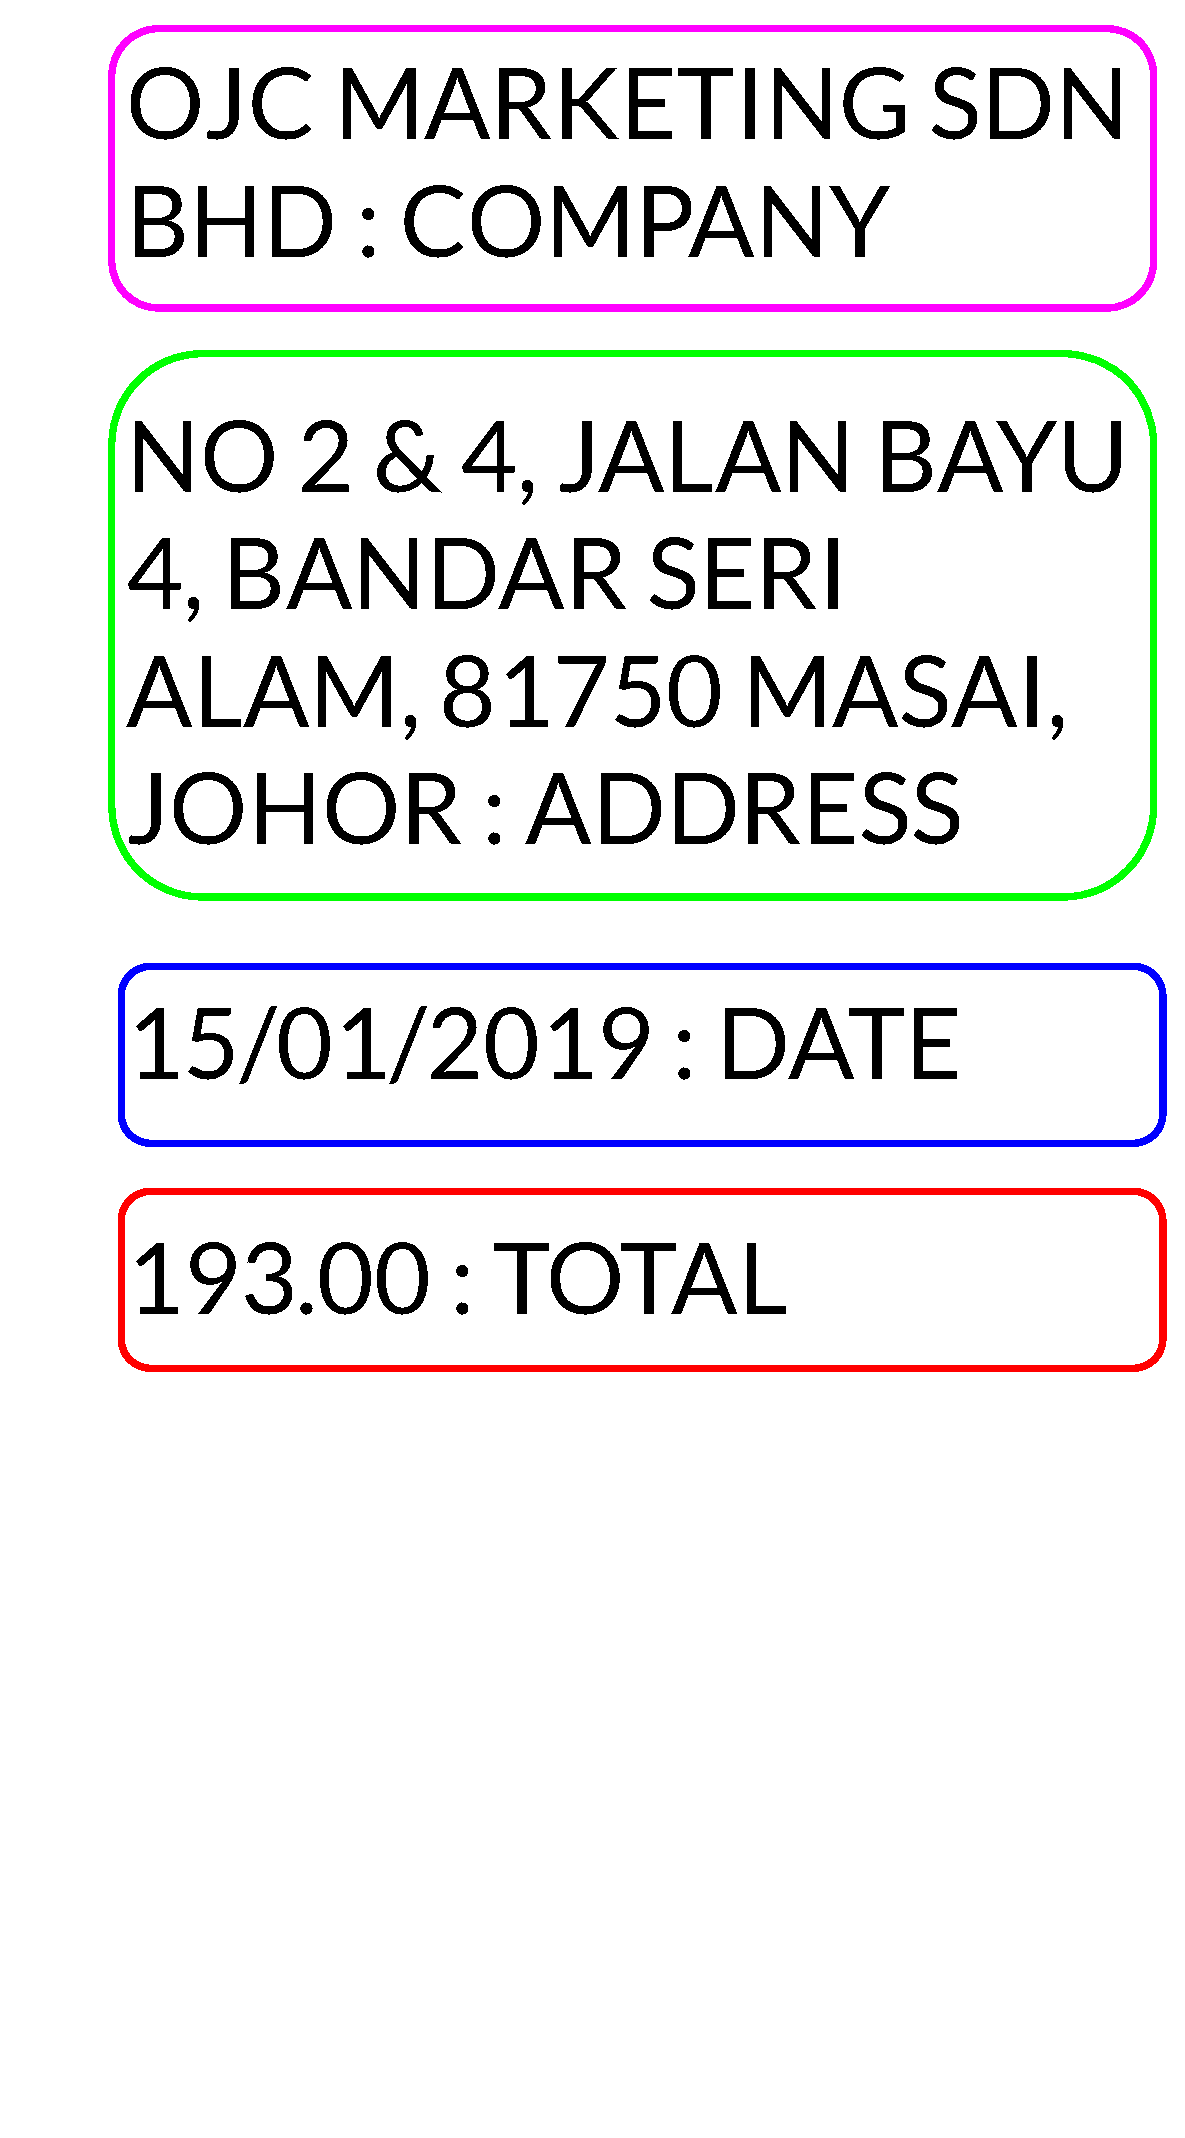
\includegraphics[width=\textwidth]{images/chapter4/sroie_output_sample2.pdf}
%         \caption{Target text}
%       \end{subfigure}
%     \caption{Example document from SROIE, accompanied by its corresponding target sequence that includes the entities to be extracted paired with their corresponding keys.}
%     \label{fig:source-target-sample}
% \end{figure}

\begin{figure}
  \centering
  \small
  \begin{subfigure}[b]{0.6\textwidth}
    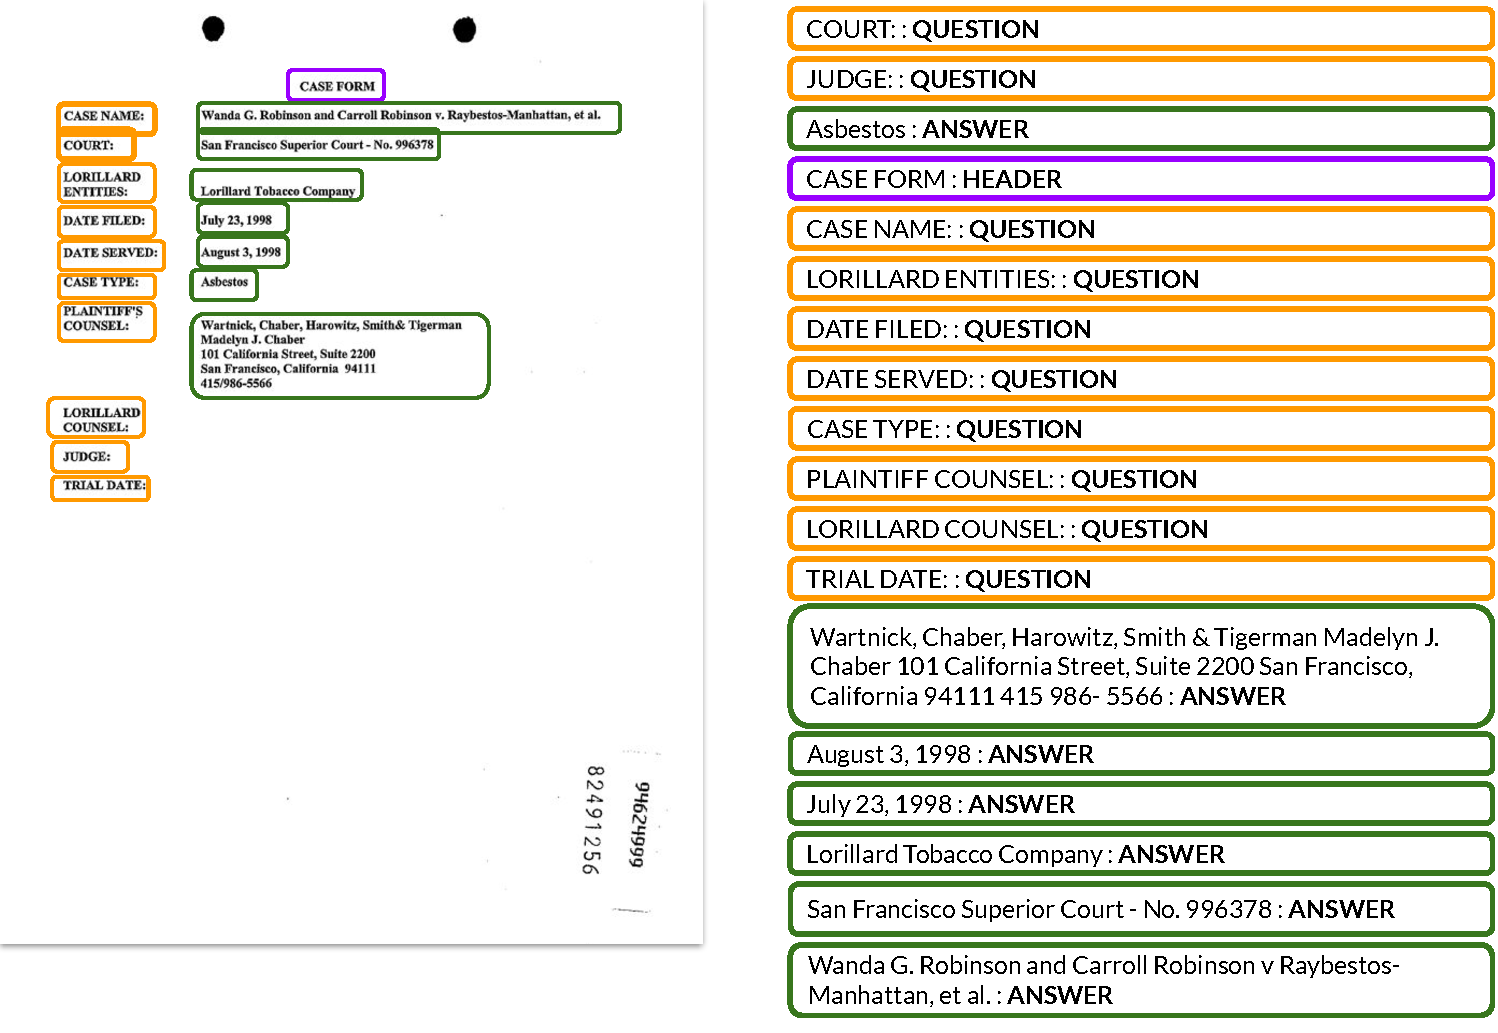
\includegraphics[width=\textwidth]{images/chapter4/funsd_sample_and_output.pdf}
    \caption{FUNSD}
  \end{subfigure}
  \begin{subfigure}[b]{0.4\textwidth}
    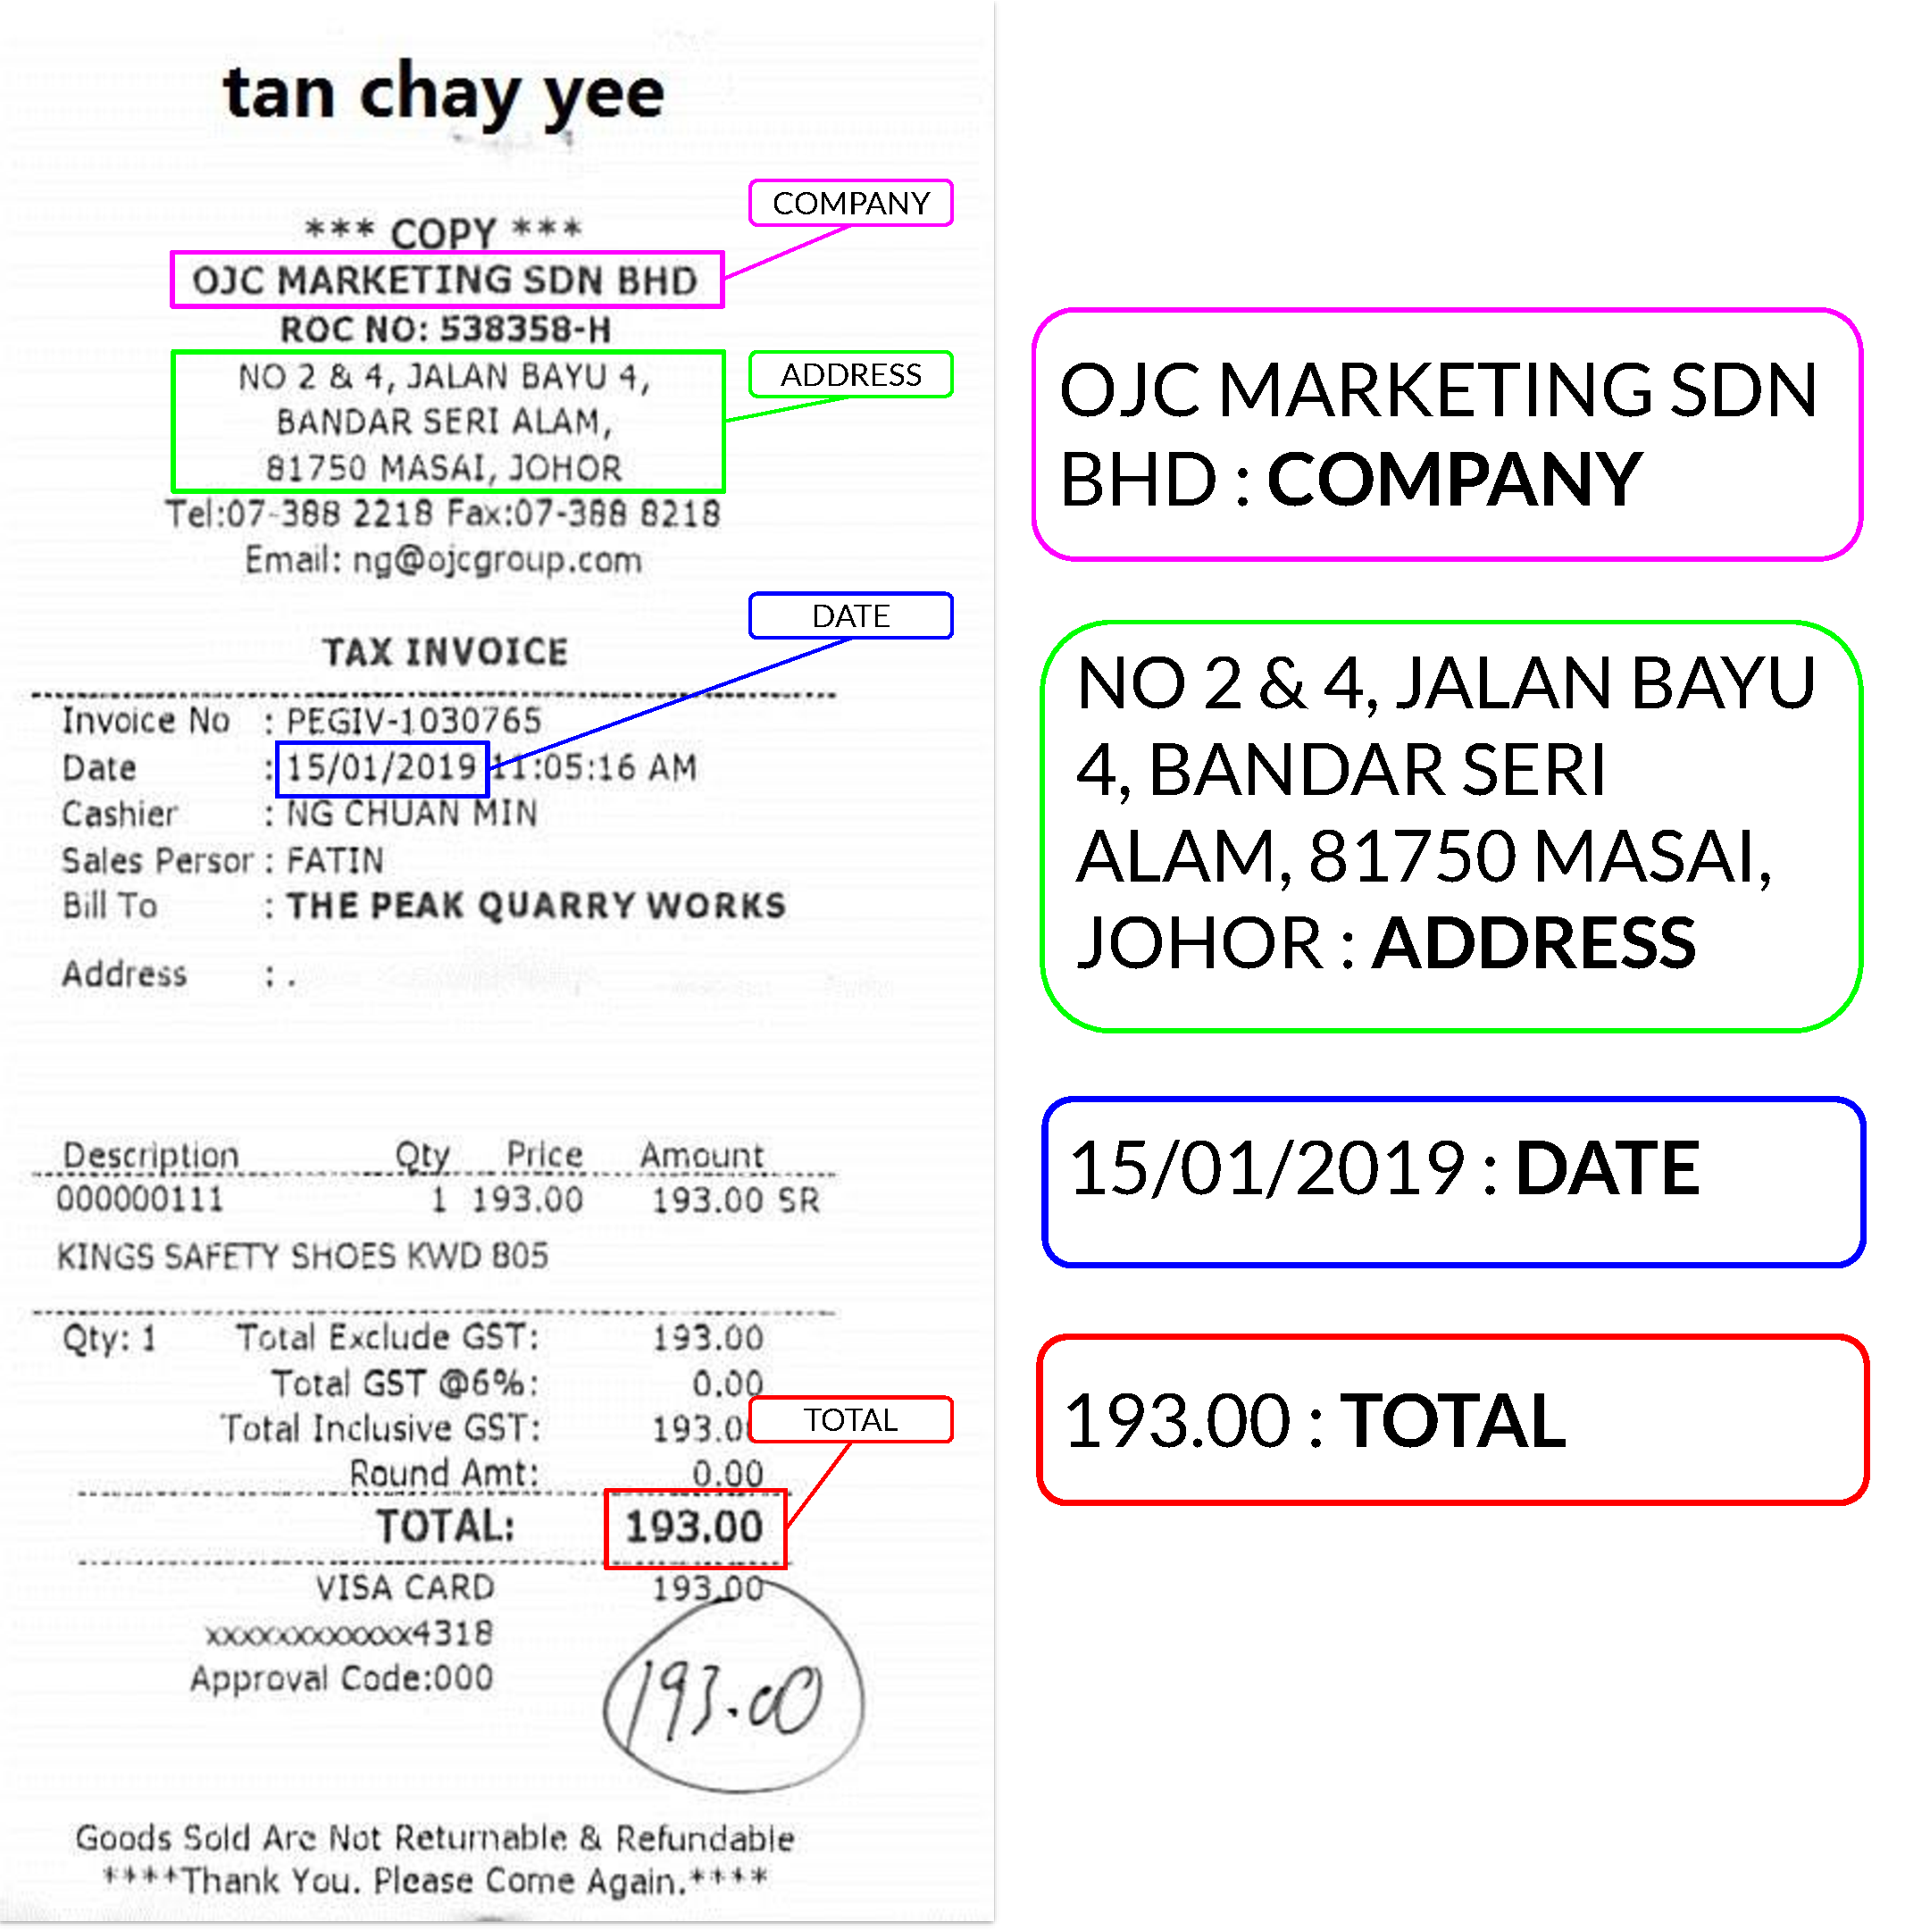
\includegraphics[width=\textwidth]{images/chapter4/sroie_sample_and_output.pdf}
    \caption{SROIE}
  \end{subfigure}
  \begin{subfigure}[b]{0.6\textwidth}
    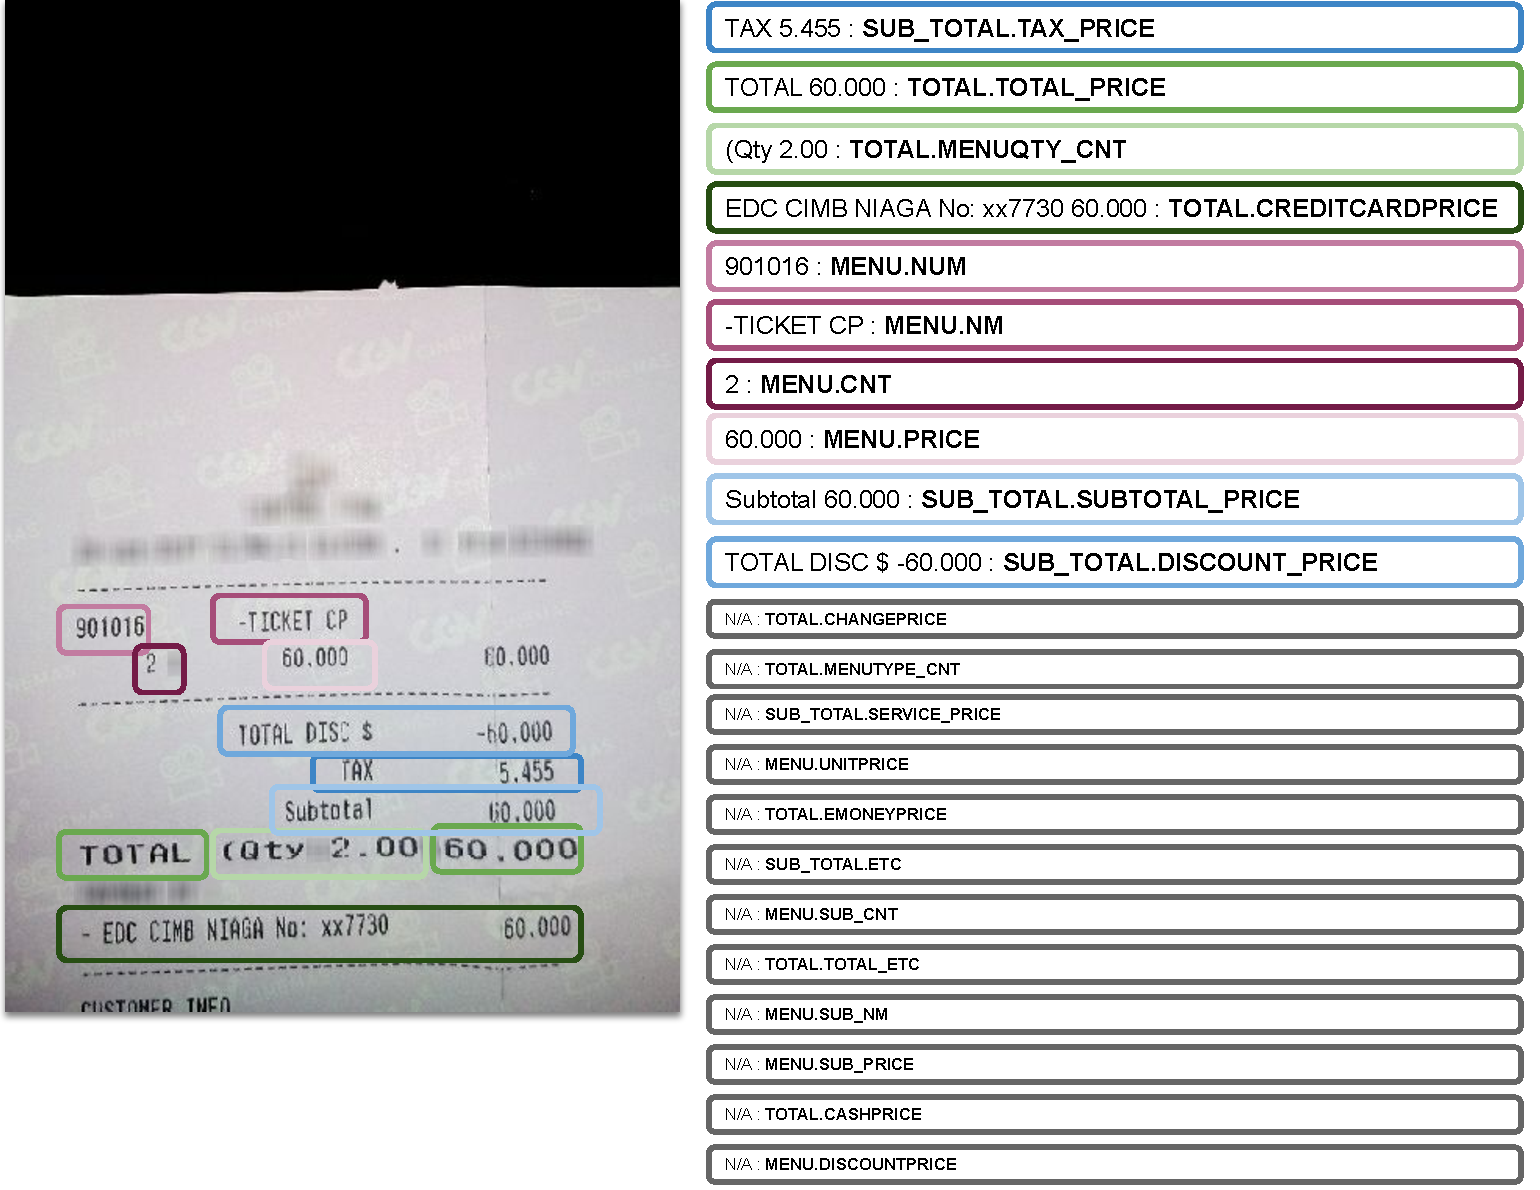
\includegraphics[width=\textwidth]{images/chapter4/cord_sample_and_output.pdf}
    \caption{CORD}
  \end{subfigure}
  \caption{Example document from FUNSD (a), SROIE (b), and CORD (c), accompanied by their corresponding target sequences that include the entities to be extracted paired with their corresponding keys.}
    \label{fig:source-target-sample}
\end{figure}

\subsection{Results and Discussion}

\subsubsection{Next Token Prediction}

\begin{table}
  \centering
  \small
  \begin{adjustbox}{max width=\textwidth}
  \begin{threeparttable}
  \begin{tabular}{cccc}
      \toprule
          Number of Layers & Pre-training Dataset & Accuracy \\ 
      \midrule
          1                & IIT-CDIP             & 67.10\%  \\
          1                & ReadingBank          & 89.37\%  \\
          2                & ReadingBank          & \textbf{95.86}\%   \\
      \bottomrule
  \end{tabular}
  \end{threeparttable}
  \end{adjustbox}
  \caption{Accuracy in predicting the next token for pairs sourced from ReadingBank, which were not used for pre-training. Selected pairs are considered "difficult", meaning that the tokens are positioned on different lines.}
  \label{table:next-token-prediction-results}
\end{table}

We evaluate the performance of the Layout2Pos module by computing the accuracy of next token prediction on a set of pairs of consecutive tokens derived from 100 examples from ReadingBank, which were not used in the pre-training phase. Specifically, we curated pairs categorized as "difficult", where the tokens are positioned on different lines, making a raster-scan approach ineffective. This choice demands the model to leverage layout information to accurately predict the next token in these scenarios.

In these experiments, we exclusively train and evaluate Layout2Pos, omitting the encoder-decoder architecture. The accuracy for each token is determined by comparing the position of the ground-truth next token in the sequence with the position of the token corresponding to the maximum logit in the generated attention scores. We vary the number of layers and the pre-training dataset used. Performance is reported in Table~\ref{table:next-token-prediction-results}. Notably, pre-training Layout2Pos on ReadingBank compared to IIT-CDIP yields an increase of over 22\% in accuracy. Additionally, our results indicate that augmenting the number of layers in Layout2Pos results in a notable increase of over 6\% in accuracy. These results highlight the significance of using documents with accurate reading orders and contextualizing layout information to produce 1D position embeddings able to capture the reading order of documents.

\subsubsection{Visual Information Extraction}

% \begin{table}
%   \centering
%   \small
%   \begin{adjustbox}{max width=\textwidth}
%   \begin{threeparttable}
%   \begin{tabular}{llccccccccccc}
%       \toprule
%           % \textbf{Model}  & & \textbf{Prec.} & \textbf{Rec.} & \textbf{F1}  & \shortstack{\textbf{Hallucination} \\ \textbf{Rate}} & \shortstack{\textbf{Repetition} \\ \textbf{Rate}} & \shortstack{\textbf{Wrong Label} \\ \textbf{Rate}} & \shortstack{\textbf{Omission} \\ \textbf{Rate}} & \shortstack{\textbf{“Other"} \\ \textbf{Rate}} \\ 
%       %     \textbf{Model}  & & \textbf{Precision} & \textbf{Recall} & \textbf{F1}  & \rotatebox{-90}{\textbf{Hallucination Rate}} & \rotatebox{-90}{\textbf{Repetition Rate}} & \rotatebox{-90}{\textbf{Wrong Label Rate}} & \rotatebox{-90}{\textbf{Omission Rate}} & \rotatebox{-90}{\textbf{“Other” Rate}} \\
%        &   & & &  & &  \multicolumn{5}{c}{\textbf{Rate}} \\ 
%        \textbf{Dataset} & \textbf{Model} & \shortstack{\textbf{Filter out}\\\textbf{Repetitions}} & \textbf{Prec.} & \textbf{Rec.} &   \textbf{F1} & \rotatebox{-90}{\textbf{Hallucination}} & \rotatebox{-90}{\textbf{Repetition}} & \rotatebox{-90}{\textbf{Wrong Label}} & \rotatebox{-90}{\textbf{Omission}} & \rotatebox{-90}{\textbf{"Other"}} \\
%       \midrule
%       \multirow{4}{*}{FUNSD} & LayoutLM  \citep{xu2020layoutlm} & \cellcolor[gray]{0.9} & 75.91 & 80.54 &	78.16 & \cellcolor[gray]{0.9} & \cellcolor[gray]{0.9} & \cellcolor[gray]{0.9} & \cellcolor[gray]{0.9} &  \cellcolor[gray]{0.9} \\
%       & LayoutLMv2-no-visual             & \cellcolor[gray]{0.9} & 78.58 &	81.49 &	80.01 & \cellcolor[gray]{0.9} & \cellcolor[gray]{0.9} & \cellcolor[gray]{0.9} & \cellcolor[gray]{0.9} &  \cellcolor[gray]{0.9} \\  
%       & BART+2D & \xmark & 75.51	& 82.95 & 79.06 &  4.08 &	10.85 &	2.59 & 25.27 & 53.20 \\
%       & BART+2D & \cmark & 75.82 &	82.95 &	79.22 & 11.57 & 10.18 & 0.00 & 24.24 & 50.01 \\ 
%       & BART+Layout2Pos & \xmark & 75.34 & 82.84 &	78.91 & 3.26 &	18.59 &	1.72 &	27.69 &	42.74 \\
%       & BART+Layout2Pos & \cmark & 75.64 & 82.84 &	79.08 & 7.68 & 18.14 & 0.00 & 26.89 & 41.28 \\
%       \midrule
%       \multirow{4}{*}{SROIE} & LayoutLM  \citep{xu2020layoutlm} & \cellcolor[gray]{0.9} & 90.74 & 93.95 & 92.32 & \cellcolor[gray]{0.9} & \cellcolor[gray]{0.9} & \cellcolor[gray]{0.9} & \cellcolor[gray]{0.9} &  \cellcolor[gray]{0.9} \\ 
%       & LayoutLMv2-no-visual             & \cellcolor[gray]{0.9} & 93.20 &	93.88 &	93.54 & \cellcolor[gray]{0.9} & \cellcolor[gray]{0.9} & \cellcolor[gray]{0.9} & \cellcolor[gray]{0.9} &  \cellcolor[gray]{0.9} \\
%       & BART+2D & \xmark & 89.61 &	93.72 &	91.62 & 1.15 &	5.00 &	6.97 &	0.00 &	12.80 \\
%       & BART+2D & \cmark & 92.06 &	93.72 & 92.88 & 1.25 &	5.60 &	0.00 &	0.00 & 13.62 \\
%       & BART+Layout2Pos & \xmark & 88.99 &	92.91 &	90.91 & 2.38 &	6.03 &	3.12 &	0.24 &	14.17 \\
%       & BART+Layout2Pos & \cmark & 90.08 &	92.91 &	91.47 & 1.03 &	6.99 &	0.00 &	0.20 &	19.16 \\
%       \midrule
%       \multirow{4}{*}{CORD} & LayoutLM  \citep{xu2020layoutlm} & \cellcolor[gray]{0.9} & 93.91 & 95.11 & 94.51 & \cellcolor[gray]{0.9} & \cellcolor[gray]{0.9} & \cellcolor[gray]{0.9} & \cellcolor[gray]{0.9} &  \cellcolor[gray]{0.9} \\ 
%       & LayoutLMv2-no-visual             & \cellcolor[gray]{0.9} & 93.14 &	94.89 &	94.00 & \cellcolor[gray]{0.9} & \cellcolor[gray]{0.9} & \cellcolor[gray]{0.9} & \cellcolor[gray]{0.9} &  \cellcolor[gray]{0.9} \\  
%       & BART+2D & \xmark \\
%       & BART+Layout2Pos & \xmark \\
%       \bottomrule
%   \end{tabular}
%   \end{threeparttable}
%   \end{adjustbox}
%   \caption{Model performance (in \%) on FUNSD, SROIE, and CORD.}
%   \label{table:visual-information-extraction-results}
% \end{table}

\begin{table}
  \centering
  \small
  \begin{adjustbox}{max width=\textwidth}
  \begin{threeparttable}
  \begin{tabular}{llcccccccccc}
      \toprule
          % \textbf{Model}  & & \textbf{Prec.} & \textbf{Rec.} & \textbf{F1}  & \shortstack{\textbf{Hallucination} \\ \textbf{Rate}} & \shortstack{\textbf{Repetition} \\ \textbf{Rate}} & \shortstack{\textbf{Wrong Label} \\ \textbf{Rate}} & \shortstack{\textbf{Omission} \\ \textbf{Rate}} & \shortstack{\textbf{“Other"} \\ \textbf{Rate}} \\ 
      %     \textbf{Model}  & & \textbf{Precision} & \textbf{Recall} & \textbf{F1}  & \rotatebox{-90}{\textbf{Hallucination Rate}} & \rotatebox{-90}{\textbf{Repetition Rate}} & \rotatebox{-90}{\textbf{Wrong Label Rate}} & \rotatebox{-90}{\textbf{Omission Rate}} & \rotatebox{-90}{\textbf{“Other” Rate}} \\
       &   & & &  & &  \multicolumn{4}{c}{\textbf{Rate}} \\ 
       \textbf{Dataset} & \textbf{Model} & & \textbf{Prec.} & \textbf{Rec.} &   \textbf{F1} & \rotatebox{-90}{\textbf{Hallucination}} & \rotatebox{-90}{\textbf{Wrong Label}} & \rotatebox{-90}{\textbf{Omission}} & \rotatebox{-90}{\textbf{"Other"}} \\
      \midrule
      \multirow{4}{*}{FUNSD} & LayoutLM  \citep{xu2020layoutlm} & & 75.91 & 80.54 &	78.16 & \cellcolor[gray]{0.9} & \cellcolor[gray]{0.9} & \cellcolor[gray]{0.9} &  \cellcolor[gray]{0.9} \\
      & LayoutLMv2-no-visual             &  & 78.58 &	81.49 &	80.01 & \cellcolor[gray]{0.9} & \cellcolor[gray]{0.9} & \cellcolor[gray]{0.9} &  \cellcolor[gray]{0.9} \\  
      & BART+2D &  & 75.82 &	82.95 &	79.22 & 11.57 & 10.18 & 24.24 & 50.01 \\ 
      & BART+Layout2Pos &  & 75.64 & 82.84 &	79.08 & 7.68 & 18.14  & 26.89 & 41.28 \\
      \midrule
      \multirow{4}{*}{SROIE} & LayoutLM  \citep{xu2020layoutlm} &  & 90.74 & 93.95 & 92.32 & \cellcolor[gray]{0.9} & \cellcolor[gray]{0.9} & \cellcolor[gray]{0.9} & \cellcolor[gray]{0.9} \\ 
      & LayoutLMv2-no-visual             &  & 93.20 &	93.88 &	93.54 & \cellcolor[gray]{0.9} & \cellcolor[gray]{0.9} & \cellcolor[gray]{0.9} &  \cellcolor[gray]{0.9} \\
      & BART+2D &  & 92.06 &	93.72 & 92.88 & 1.25 &0.00 & 13.62 & 5.60 \\
      & BART+Layout2Pos &  & 90.08 &	92.91 &	91.47 & 1.03 & 0.20 &	19.16 &	6.99 \\
      \midrule
      \multirow{4}{*}{CORD} & LayoutLM  \citep{xu2020layoutlm} & & 93.91 & 95.11 & 94.51 & \cellcolor[gray]{0.9} & \cellcolor[gray]{0.9} & \cellcolor[gray]{0.9} & \cellcolor[gray]{0.9}  \\ 
      & LayoutLMv2-no-visual             & & 93.14 &	94.89 &	94.00 & \cellcolor[gray]{0.9} & \cellcolor[gray]{0.9} & \cellcolor[gray]{0.9} &  \cellcolor[gray]{0.9} \\  
      & BART+2D &  \\
      & BART+Layout2Pos &  \\
      \bottomrule
  \end{tabular}
  \end{threeparttable}
  \end{adjustbox}
  \caption{Model performance (in \%) on FUNSD, SROIE, and CORD.}
  \label{table:visual-information-extraction-results}
\end{table}


Table~\ref{table:visual-information-extraction-results} reports the performance of all four models on FUNSD, SROIE, and CORD.


\section{Conclusion}
	\cleardoublepage
	\let\leftmark=\oldleftmark

        \acresetall
	
\chapter{A Layout-Aware Multimodal Benchmark for Long Document Summarization}
\label{chapter:chapter5}

\renewcommand{\leftmark}{\spacedlowsmallcaps{A Long and Layout-Aware Multimodal Benchmark for Text Summarization}}

\begin{chapabstract}
    {\em
    Text Summarization is a popular task and an active area of research for the \ac{NLP} community. It requires accounting for long input texts, a characteristic which poses computational challenges for neural models. 
    Moreover, real-world documents come in a variety of complex, visually-rich, layouts. This information is of great relevance, whether to highlight salient content or to encode long-range interactions between textual passages. Yet, all publicly available summarization datasets only provide plain text content.
    To facilitate research on how to exploit visual/layout information to better capture long-range dependencies in summarization models, we present \textit{LoRaLay}, a collection of datasets for long-range summarization with accompanying visual/layout information. We extend existing and popular English datasets (arXiv and PubMed) with visual/layout information and propose four novel datasets -- consistently built from scholar resources -- covering French, Spanish, Portuguese, and Korean languages.
    Further, we propose new baselines merging layout-aware and long-range models -- two orthogonal approaches -- and obtain state-of-the-art results, showing the importance of combining both lines of research.
    \vspace*{5mm}
    The work in this chapter has led to the publication of a conference paper:}
    \begin{itemize}
        \item \small \fullcite{nguyen-etal-2023-loralay}.
    \end{itemize}
\end{chapabstract}

\ifthenelse{\boolean{skipCh5}}{\endinput}{}


\newpage

\minitoc
\chapterwithfigures{\nameref*{chapter:chapter5}}
\chapterwithtables{\nameref*{chapter:chapter5}}

Long document understanding presents several significant challenges. Firstly, contemporary document understanding approaches are based on the Transformer architecture \citep{vaswani2017attention}. However, the quadratic complexity inherent to self-attention renders them unable to capture long-range dependencies, hence constraining their use to short sequences. Secondly, understanding long documents requires the ability to effectively model all information, encompassing not only text but also other modalities such as layout information. Although LayoutLM \citep{xu2020layoutlm} has shown substantial improvements in short document understanding tasks, efficiently leveraging long multimodal information to understand long documents remains an unresolved and under-explored problem.

In this work, we aim at spurring further research on how to incorporate multimodal information to better capture long-range dependencies. To develop models capable of exploiting multimodal information from long documents, there is a need for tasks and datasets that cover every modality. Focusing on compressing the most relevant information from long texts to short summaries, the Text Summarization task naturally lends itself to benefit from a global context. Notice that, in practice, the limitations linked to sequence length are also amplified by the lack of visual/layout information in the existing datasets. 

Yet, the vast majority of publicly available summarization datasets only provide plain text content. \citet{hermann2015teaching} proposed the CNN/DailyMail dataset, a collection of English articles extracted from the CNN and The Daily Mail portals. Each news article is associated with multi-sentence highlights which serve as reference summaries. \citet{scialom2020mlsum} bridge the gap between English and non-English resources for text summarization by introducing MLSum, a large-scale multilingual summarization corpus providing news articles written in French, German, Spanish, Turkish and Russian. Going toward more challenging scenarios involving significantly longer documents, the arXiv and PubMed datasets \citep{cohan2018discourse} consist of scientific articles collected from academic repositories, wherein the paper abstracts are used as summaries. To encourage a shift towards building more abstractive summarization models with global content understanding, \citet{sharma2019bigpatent} introduce BIGPATENT, a large-scale dataset made of U.S. patent filings, where invention descriptions serve as reference summaries. As opposed to other \ac{DU} tasks (e.g., form understanding, \ac{Document VQA}) in which the placement of text on the page and/or visual components are the main source of information needed to find the desired data \citep{borchmann2021due}, text plays a predominant role in document summarization. However, guidelines for summarizing texts -- especially long ones -- often recommend roughly previewing them to break them down into their major sections \citep{toprak2009three, luo2019reading}. \citet{miculicich2022document} propose a two-stage method which detects text segments and incorporates this information in an extractive summarization model. \citet{cao2022hibrids} collect a new dataset for long and structure-aware document summarization, consisting of 21k documents written in English and extracted from WikiProject Biography. 

Although not all documents are explicitly organized into clearly defined sections, the great majority contains layout and visual clues (e.g., a physical organization into paragraphs, bigger headings/subheadings) which help structure their textual contents and facilitate reading. Thus, we argue that layout is crucial to summarize long documents. We present \emph{LoRaLay}, a collection of datasets designed for long-range and layout-aware summarization. LoRaLay is a large-scale corpus of research papers that extends two popular datasets, arXiv and PubMed, with layout and visual information, and introduces 4 novel datasets covering French, Spanish, Portuguese and Korean languages. Finally, LoRaLay is accompanied by novel baselines that combine long-range and layout-aware models to provide enhanced performance.

In this chapter, we first detail the dataset construction process. Then, we introduce novel long-range and layout-aware baselines and offer a detailed explanation of the experimental setup. Lastly, we demonstrate the importance of combining layout-aware and long-range modeling through qualitative and quantitative evaluations.

\section{Datasets Construction}

Inspired by the way the arXiv and PubMed datasets were built \citep{cohan2018discourse}, we construct our corpus from research papers, with abstracts as ground-truth summaries. As the PDF format allows simultaneous access to textual, visual and layout information, we collect PDF files to construct our datasets, and provide their URLs.\footnote{We make the corpus-construction code publicly available at \url{https://github.com/recitalAI/loralay-datasets}.}

For each language, we select a repository that contains a high number of academic articles (in the order of hundreds of thousands) and provides easy access to abstracts. 
More precisely, we chose the following repositories:
\begin{itemize}
    \item Archives Ouverte HAL (French),\footnote{\url{https://hal.archives-ouvertes.fr/}} an open archive of scholarly documents from all academic fields. As HAL is primarily directed towards French academics, a great proportion of articles are written in French;
    \item SciELO (Spanish and Portuguese),\footnote{\url{https://www.scielo.org/}} an open access database of academic articles published in journal collections from Latin America, Iberian Peninsula and South Africa, and covering a broad range of topics (e.g. agricultural sciences, engineering, health sciences, letters and arts). Languages include English, Spanish, and Portuguese.
    \item KoreaScience (Korean),\footnote{\url{http://www.koreascience.or.kr}} an open archive of Korean scholarly publications in the fields of natural sciences, life sciences, engineering, and humanities and social sciences. Articles are written in English or Korean.
\end{itemize}

Further, we provide enhanced versions of the arXiv and PubMed datasets, respectively denoted as arXiv-Lay and PubMed-Lay, for which layout information is provided.

\begin{figure}[ht]
\centering
    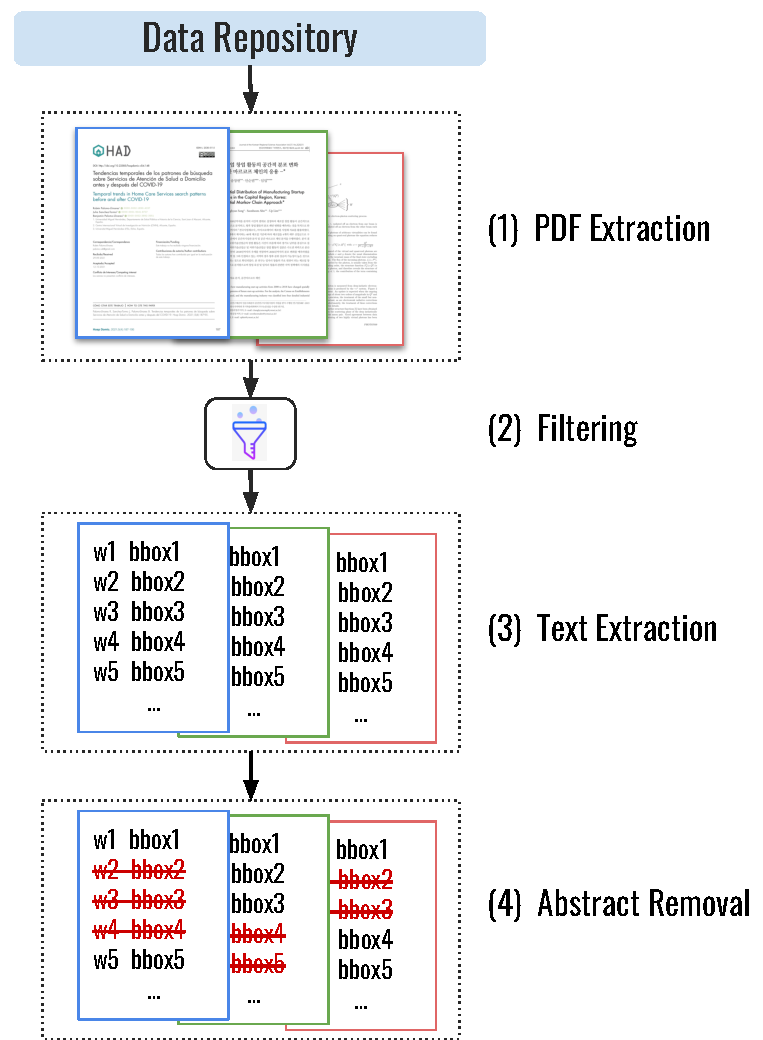
\includegraphics[width=0.45\textwidth]{images/chapter5/Dataset_Construction_Process.pdf}
  \caption{Dataset Construction Process.}
  \label{fig:chapter5-dataset-construction}
\end{figure}

The dataset construction process is illustrated in Figure~\ref{fig:chapter5-dataset-construction}. 

\subsection{Collecting the Data}

\subsubsection{Extended Datasets}

The arXiv and PubMed datasets \cite{cohan2018discourse} contain long scientific research papers extracted from the arXiv and PubMed repositories. We augment them by providing their PDFs, allowing access to layout and visual information. As the abstracts contained in the original datasets are all lowercased, we do not reuse them, but rather extract the raw abstracts using the corresponding APIs.

Note that we were unable to retrieve all the original documents. For the most part, we failed to retrieve the corresponding abstracts, as they did not necessarily match the ones contained in the PDF files (due to \textit{e.g.} PDF-parsing errors). We also found that some PDF files were unavailable, while others were corrupted or scanned documents. Figure~\ref{fig:chapter5-details-lost-docs} provides details on the amount of original documents lost in the process of augmenting arXiv and PubMed with layout/visual information. We observe four types of failures, and provide numbers for each type: 

\begin{itemize}
    \item The link to the document's PDF file is not provided (\textit{Unavailable PDF});
    \item The PDF file is corrupted (i.e., cannot be opened) (\textit{Corrupted PDF});
    \item The document is not digital-born, making it impossible to parse it with PDF parsing tools (\textit{ Scanned PDF});
    \item The document's abstract cannot be found in the PDF (\textit{Irretrievable Abstract}).
\end{itemize}

\begin{figure}[H]
    \centering
  \begin{subfigure}[b]{0.4\textwidth}
    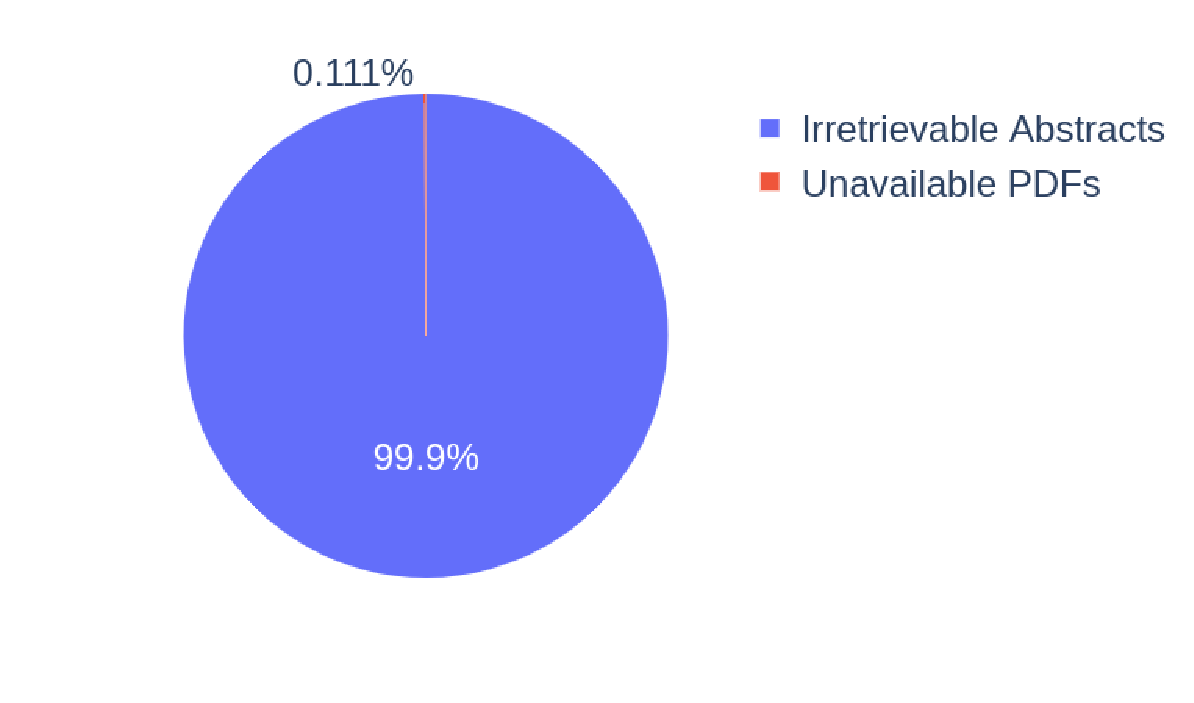
\includegraphics[width=0.8\textwidth]{images/chapter5/distribution_failure_types_arxiv.pdf}
  \end{subfigure}
  \begin{subfigure}[b]{0.4\textwidth}
    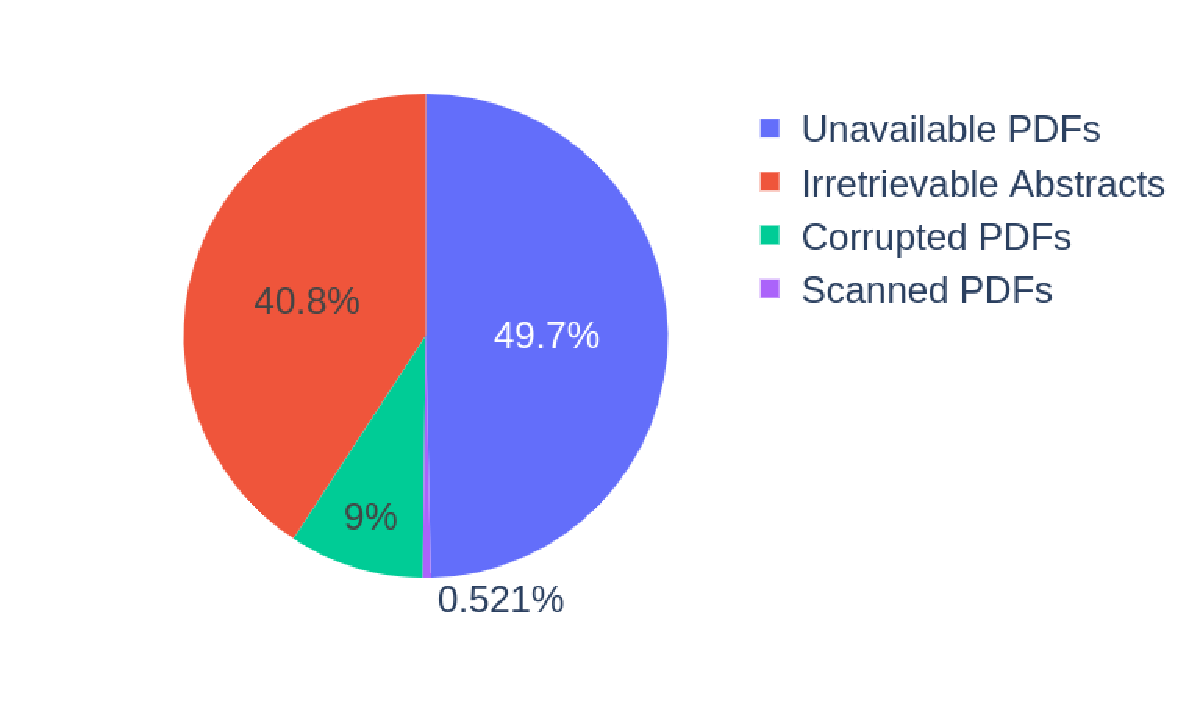
\includegraphics[width=0.8\textwidth]{images/chapter5/distribution_failure_types_pubmed.pdf}
  \end{subfigure}
\caption{Distribution of failure types in arXiv-Lay (top) and PubMed-Lay (bottom).}
\label{fig:chapter5-details-lost-docs}
\end{figure}

In total, about 39\% (35\%) of the original documents in arXiv (PubMed) were lost.

\paragraph{arXiv-Lay}

The original arXiv dataset \citep{cohan2018discourse} was constructed by converting the \LaTeX~ files to plain text. To be consistent with the other datasets -- for which \LaTeX~files are not available -- we instead use the PDF files to extract both text and layout elements. For each document contained in the original dataset, we fetch (when possible) the corresponding PDF file using Google Cloud Storage buckets. As opposed to the original procedure, we do not remove tables nor discard sections that follow the conclusion. We retrieve the corresponding abstracts from a metadata file provided by Kaggle.\footnote{\url{https://www.kaggle.com/Cornell-University/arxiv}}

\paragraph{PubMed-Lay}

For PubMed, we use the PMC OAI Service\footnote{\url{https://www.ncbi.nlm.nih.gov/pmc/tools/oai/}} to retrieve abstracts and PDF files. 

\subsubsection{New Datasets}

\paragraph{HAL}

We use the HAL API\footnote{\url{https://api.archives-ouvertes.fr/docs/search}} to download research papers written in French. To avoid excessively long (e.g. theses) or short (e.g. posters) documents, extraction is restricted to journal and conference papers. 

\paragraph{SciELO}

Using Scrapy,\footnote{\url{https://scrapy.org/}} we crawl the following SciELO collections: Ecuador, Colombia, Paraguay, Uruguay, Bolivia, Peru, Portugal, Spain and Brazil. We download documents written either in Spanish or Portuguese, according to the metadata, obtaining two distinct datasets: SciELO-ES (Spanish) and SciELO-PT (Portuguese).

\paragraph{KoreaScience}

Similarly, we scrape the KoreaScience website to extract research papers. We limit search results to documents whose publishers’ names contain the word \emph{Korean}. This rule was designed after sampling documents in the repository, and is the simplest way to get a good proportion of papers written in Korean. We show that this rule does not bias the sample towards a specific research area. We compute the distribution of topics covered by all publishers, and compare it to the distribution of topics covered by publishers whose name contains the word \textit{Korean}. Figure~\ref{fig:chapter5-distr-koreascience-topics} shows that the distribution obtained using our rule remains roughly the same as the original. Further, search is restricted to papers published between 2012 and 2021, as recent publications are more likely to have digital-born, searchable PDFs. Finally, we download the PDF files of documents that contain an abstract written in Korean. 

\begin{figure}[ht]
\centering
    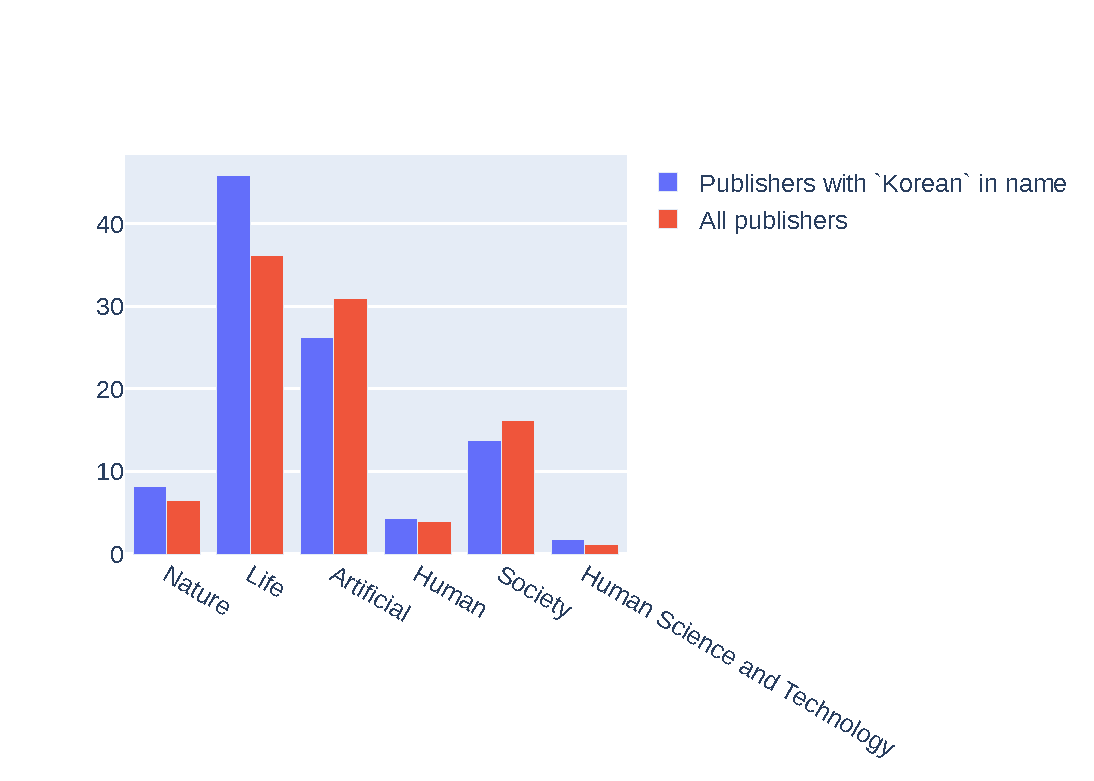
\includegraphics[width=0.8\textwidth]{images/chapter5/koreascience_topic_distr.pdf}
  \caption{Distribution of topics covered by all publishers (red) vs distribution of topics covered by publishers whose name contains the word \textit{Korean} (blue).}
  \label{fig:chapter5-distr-koreascience-topics}
\end{figure}

\subsection{Data Pre-processing}

For each corpus, we use the 95th percentile of the page distribution as an upper bound to filter out documents with too many pages, while the 5th (1st for HAL and SciELO) percentile of the summary length distribution is used as a minimum threshold to remove documents whose abstracts are too short. As our baselines do not consider visual information, we only extract text and layout from the PDF files. Layout is incorporated by providing the spatial position of each word in a document page image, represented by its bounding box $(x_0, y_0, x_1, y_1)$, where $(x_0, y_0)$ and $(x_1, y_1)$ respectively denote the coordinates of the top-left and bottom-right corners. Using the PDF rendering library Poppler\footnote{ \url{https://poppler.freedesktop.org/}}, text and word bounding boxes are extracted from each PDF, and the sequence order is recovered based on heuristics around the document layout (e.g., tables, columns). Abstracts are then removed by searching for exact matches; when no exact match is found, we use \texttt{fuzzysearch}\footnote{ \url{https://pypi.org/project/fuzzysearch/}} and \texttt{regex}\footnote{ \url{https://pypi.org/project/regex/}} to find near matches. We use a maximum Levenshtein distance of 20 with fuzzysearch, and a maximum number of errors of 3 with regex. For the non-English datasets, documents might contain several abstracts, written in different languages. To avoid information leakage, we retrieve the abstract of each document in every language available -- according to the API for HAL or the websites for SciELO and KoreaScience -- and remove them using the same strategy as for the main language. In the case an abstract cannot be found, we discard the document to prevent any unforeseen leakage. 

\subsection{Datasets Statistics}

The statistics of our proposed datasets, along with those computed on existing summarization datasets of long documents \citep{cohan2018discourse, sharma2019bigpatent} are reported in Table~\ref{tab:chapter5-datasets-stats}. We see that document lengths are comparable or greater than for the arXiv, PubMed and BigPatent datasets.  

For arXiv-Lay and PubMed-Lay, we retain the original train/validation/splits and try to reconstruct them as faithfully to the originals as possible. For the new datasets, we order documents based on their publication dates and provide splits following a chronological ordering. For HAL and KoreaScience, we retain 3\% of the articles as validation data, 3\% as test, and the remaining as training data. To match the number of validation/test documents in HAL and KoreaScience, we split the data into 90\% for training, 5\% for validation and 5\% for test, for both SciELO datasets. The statistics of our splits are provided in Table~\ref{tab:chapter5-splits-stats}

\begin{table}
\centering
\small
% \resizebox{0.5\linewidth}{!}{%
\begin{tabular}{ccccc}
\hline
             \multirow{3}{*}{\textbf{Dataset}} & \textbf{\# Docs} & \textbf{Mean}         & \textbf{Mean}  \\
             &                  & \textbf{Article}        & \textbf{Summary} \\
             &                  & \textbf{Length}        & \textbf{Length} \\
             \hline
arXiv \citep{cohan2018discourse}      & 215,913   & 3,016 & 203  \\
PubMed \citep{cohan2018discourse}     & 133,215   & 4,938 & 220   \\
BigPatent \citep{sharma2019bigpatent} & 1,341,362 & 3,572 & 117 \\
\midrule
arXiv-Lay       & 130,919 & 7,084 & 125 \\
PubMed-Lay      & 86,668  & 4,038 & 144 \\
HAL          & 46,148  & 4,543 & 134 \\
SciELO-ES    & 23,170  & 4,977 & 172 \\
SciELO-PT    & 21,563  & 6,853 & 162 \\
KoreaScience & 37,498  & 3,192 &  95 \\
\hline
\end{tabular}
% }
\caption{Datasets statistics. Article and summary lengths are computed in words. For KoreaScience, words are obtained via white-space tokenization. Difference between arXiv and arXiv-Lay is due to the fact that we retain the whole document, while \citet{cohan2018discourse} truncate it after the conclusion.}
\label{tab:chapter5-datasets-stats}
\end{table}

\begin{table}[]
\centering
\small 
\resizebox{\linewidth}{!}{%
\begin{threeparttable}
\begin{tabular}{crrrrrrrrrr}
\hline
\multicolumn{1}{c}{\multirow{2}{*}{\textbf{Dataset}}} & & \multicolumn{3}{c}{\textbf{Instances}} &                                                  & \multicolumn{2}{c}{\textbf{Input Length}} & & \multicolumn{2}{c}{\textbf{Output Length}} \\
\multicolumn{1}{l}{} & & \multicolumn{1}{c}{\textbf{Train}} & \multicolumn{1}{c}{\textbf{Dev}} & \multicolumn{1}{c}{\textbf{Test}} & & \textbf{Median}         & \textbf{90\%-ile}        & & \textbf{Median}         & \textbf{90\%-ile}         \\
\hline
arXiv \citep{cohan2018discourse}  & & 203,037 & 6,436 & 6,440 & & 6,151 & 14,405 & & 171 & 352 \\
PubMed \citep{cohan2018discourse} & & 119,924 & 6,633 & 6,658 & & 2,715 &  6,101 & & 212 & 318 \\
\midrule
arXiv-Lay               & & 122,189                   & 4,374                   & 4,356      &              &  6,225         & 12,541           &   & 150          & 249     \\
PubMed-Lay              & & 78,234                    & 4,084                   & 4,350      &              & 
3,761        & 7,109           &  & 182           & 296              \\
HAL                  & & 43,379                    & 1,384                   & 1,385      &              & 4,074          & 8,761           & & 179            & 351              \\
SciELO-ES            & & 20,853                    & 1,158                   & 1,159      &               & 4,859          & 8,519           & & 226            & 382              \\
SciELO-PT            & & 19,407                    & 1,078                   & 1,078      &               &  6,090          & 9,655           &  & 239                &  374                \\
KoreaScience         & & 35,248                    & 1,125                   & 1,125      &              &  2,916          &  5,094           &  & 219           & 340   \\
\hline 
\end{tabular}
\end{threeparttable}
}
\caption{Datasets splits and statistics. Input and output lengths are computed in tokens, obtained using Pegasus and mBART-50's tokenizers for the English and non-English datasets, respectively.}
\label{tab:chapter5-splits-stats}
\end{table}

The distribution of research areas in arXiv-Lay and HAL are provided in Figures~\ref{fig:chapter5-arxiv-research-areas} and ~\ref{fig:chapter5-hal-research-areas}, respectively. Such distributions are not available for the other datasets, as we did not have access to topic information during extraction.

\begin{figure}[H]
    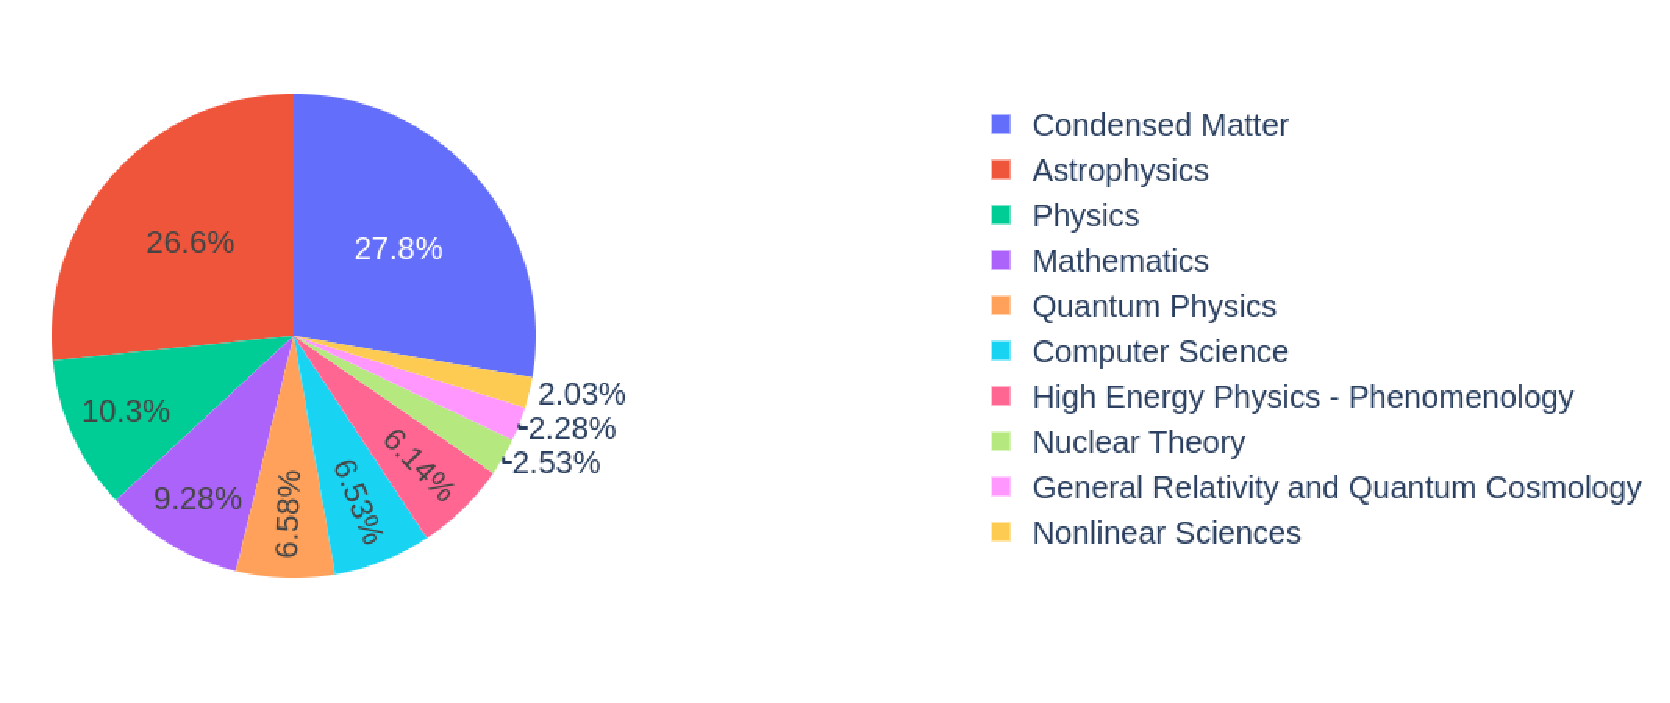
\includegraphics[width=0.5\textwidth]{images/chapter5/distribution_research_areas_arxiv.pdf}
  \caption{Distribution of research areas in arXiv-Lay.}
  \label{fig:chapter5-arxiv-research-areas}
\end{figure}

\begin{figure}[H]
    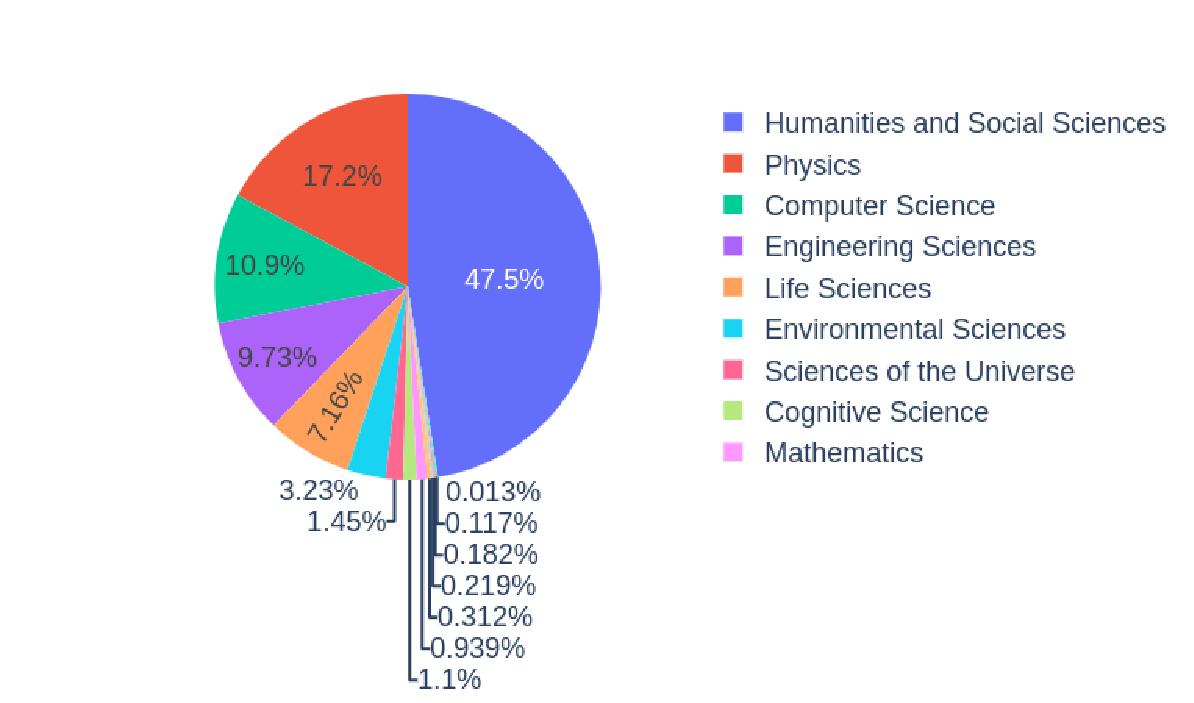
\includegraphics[width=0.5\textwidth]{images/chapter5/distribution_research_areas_hal.pdf}
  \caption{Distribution of research areas in HAL.}
  \label{fig:chapter5-hal-research-areas}
\end{figure}


\section{Experiments}

\subsection{Models}

We provide baseline models for abstractive summarization, built on the Transformer architecture. These models are categorized into four groups: text-only models with standard input size, layout-aware models with standard input size, long-range text-only models, and long-range layout-aware models. For reproducibility purposes, we make the models' implementation, along with the fine-tuning and evaluation scripts, publicly available.\footnote{\url{https://github.com/recitalAI/loralay-modeling}}

We do not explore the use of visual information in long document summarization, as the focus is on evaluating baseline performance using state-of-the-art summarization models augmented with layout information. While visual features might provide a better understanding of structures such as tables and figures, we do not expect substantial gains with respect to layout-aware models. Indeed, the information provided in figures (i.e., information that cannot be captured by layout or text) are commonly described in the caption or related paragraphs. 

\paragraph{Text-only Models with Standard Input Size}

We use Pegasus \citep{zhang2020pegasus} as a text-only baseline for arXiv-Lay and PubMed-Lay. Pegasus is an encoder-decoder model pre-trained using gap-sentences generation, making it a state-of-the-art model for abstractive summarization.
For the non-English datasets, we rely on a finetuned mBART as our baseline. mBART \citep{liu2020multilingual} is a multilingual sequence-to-sequence model pretrained on large-scale monolingual corpora in many languages using the BART objective \citep{lewis2019bart}. We use its extension, mBART-50 \citep{tang2020multilingual},\footnote{For the sake of clarity, we refer to mBART-50 as mBART.} which is created from the original mBART by extending its embeddings layers and pre-training it on a total of 50 languages. 
Both Pegasus and mBART are limited to a maximum sequence length of 1,024 tokens, which is well below the median length of each dataset.

\paragraph{Layout-aware Models with Standard Input Size}

We introduce layout-aware extensions of Pegasus and mBART, respectively denoted as Pegasus+Layout and mBART+Layout. Following LayoutLM \citep{xu2020layoutlm}, each token bounding box coordinates $(x_0, y_0, x_1, y_1)$ is normalized into an integer in the range [0, 1000]. Spatial positions are encoded using four embedding tables, namely two for the coordinate axes ($x$ and $y$), and the other two for the bounding box size (width and height). The layout representation of a token is formed by summing the resulting embedding representations
The final representation of a token is then obtained through point-wise summation of its textual, 1D-positional and layout embeddings.

\paragraph{Long-range, Text-only Models}

To process longer sequences, we leverage BigBird \citep{zaheer2020big}, a sparse-attention based Transformer which reduces the quadratic dependency to a linear one. For arXiv-Lay and PubMed-Lay, we initialize BigBird from Pegasus \citep{zaheer2020big} and for the non-English datasets, we use the weights of mBART. The resulting models are referred to as BigBird-Pegasus and BigBird-mBART. For both models, BigBird sparse attention is used only in the encoder. Both models can handle up to 4,096 inputs tokens, which is greater than the median length in PubMed-Lay, HAL and KoreaScience. 


\paragraph{Long-range, Layout-aware Models}

We also include layout information in long-range text-only models. Similarly to layout-aware models with standard input size, we integrate layout information into our long-range models by encoding each token's spatial position in the page. The resulting models are denoted as BigBird-Pegasus+Layout and BigBird-mBART+Layout.


\paragraph{Additional State-of-the-Art Baselines}

We further consider additional state-of-the-art baselines for summarization: i) the text-only T5 \citep{raffel2020exploring} with standard input size, ii) the long-range Longformer-Encoder-Decoder (LED) \citep{beltagy2020longformer}, and iii) the layout-aware, long-range LED+Layout, which we implement similarly to the previous layout-aware models.

\subsection{Implementation Details}

We initialize our Pegasus-based and mBART-based models with, respectively, the google/pegasus-large and facebook/mbart-large-50 checkpoints shared through the Hugging Face Model Hub. As for T5 and LED, we use the weights from t5-base and allenai/led-base-16384, respectively.\footnote{The large versions of T5 and LED did not fit into GPU due to their size.}

Following \citet{zhang2020pegasus} and \citet{zaheer2020big}, we fine-tune our models up to 74k (100k) steps on arXiv-Lay (PubMed-Lay). On HAL, the total number of steps is set to 100k, while it is decreased to 50k for the other non-English datasets. We tested different values for the number of steps (10k, 25k, 50k, 100k) and chose the one that gave the best validation scores for mBART.
For each model, we select the checkpoint with the best validation loss. For Pegasus and mBART models, inputs are truncated at 1,024 tokens. For BigBird-Pegasus models, we follow \citet{zaheer2020big} and set the maximum input length at 3,072 tokens. As the median input length is much greater in almost every non-English dataset, we increase the maximum input length to 4,096 tokens for BigBird-mBART models. Output length is restricted to 256 tokens for all models, which is enough to fully capture at least 50\% of the summaries in each dataset.

For evaluation, we use beam search and report a single run for each model and dataset. Following \citet{zhang2020pegasus, zaheer2020big}, we set the number of beams to 8 for Pegasus-based models, and 5 for BigBird-Pegasus-based models. For the non-English datasets, we set it to 5 for all models, for fair comparison. For all experiments, we use a length penalty of 0.8. 

Models were implemented in Python using PyTorch \citep{paszke2017automatic} and Hugging Face \citep{wolf2019huggingface} librairies. In all experiments, we use Adafactor \citep{shazeer2018adafactor}, a stochastic optimization method based on Adam \citep{kingma2014adam} that reduces memory usage while retaining the empirical benefits of adaptivity. We set a learning rate warmup over the first 10\% steps -- except on arXiv-Lay where it is set to 10k consistently with \citet{zaheer2020big}, and use a square root decay of the learning rate. All our experiments have been run on four Nvidia V100 with 32GB each. 

\section{Results and Discussion}

\subsection{General Results}

% \begin{table}[ht]
% \centering
% \small
% \begin{tabular}{lccc}
% \toprule
% \multicolumn{1}{c}{\textbf{Model}} & \textbf{\# Params} & \shortstack{\textbf{arXiv/} \\ \textbf{arXiv-Lay}} & \shortstack{\textbf{PubMed/} \\ \textbf{PubMed-Lay}} \\  
% \midrule
%  \rowcolor{Gray} Pegasus \citep{zhang2020pegasus} & 568M & 38.83 & 41.34 \\
%  \rowcolor{Gray} BigBird-Pegasus \citep{zaheer2020big} & 576M & 41.77 & 42.33\\
% \hline
% T5 \citep{raffel2020exploring}                     & 223M & 37.90 & 39.23 \\ 
% LED \citep{beltagy2020longformer}                   & 161M & 40.74 & 41.54 \\ 
% LED+Layout             & 165M & 40.96 & 41.83 \\[0.7mm]
% Pegasus                & 568M & 39.07 & 39.75 \\ 
% Pegasus+Layout         & 572M & 39.25 & 39.85 \\
% BigBird-Pegasus        & 576M & 39.59 & 41.09 \\
% BigBird-Pegasus+Layout & 581M & \textbf{41.15} & \textbf{42.05} \\
% \bottomrule
                            
% \end{tabular}
% % }
% \caption{ROUGE-L scores on arXiv-Lay and PubMed-Lay. Reported results obtained by Pegasus and BigBird-Pegasus on the original arXiv and PubMed are reported with a gray background. The best results obtained on arXiv-Lay and PubMed-Lay are denoted in bold.}
% \label{tab:chapter5-rl-scores-arxiv-pubmed}
% \end{table}

\begin{table}[ht]
\centering
\small
\begin{tabular}{l*{13}{c}}
\toprule
\multicolumn{1}{c}{\multirow{2}{*}{\textbf{Model}}} & \textbf{\# Params} & \multicolumn{3}{c}{\shortstack{\textbf{arXiv/} \\ \textbf{arXiv-Lay}}}  &                                               & \multicolumn{3}{c}{\shortstack{\textbf{PubMed/} \\ \textbf{PubMed-Lay}}} \\ \cline{3-5} \cline{7-9} 
\multicolumn{1}{l}{}               &  & \multicolumn{1}{c}{R-1} & \multicolumn{1}{c}{R-2} & \multicolumn{1}{c}{R-L} & & R-1     & R-2     & R-L \\ 
\midrule
\rowcolor{Gray} Pegasus \citep{zhang2020pegasus}             & 568M & 44.21 & 16.95 & 38.83 & & 45.97 & 20.15 & 41.34 \\  
\rowcolor{Gray} BigBird-Pegasus \citep{zaheer2020big}        & 576M & 46.63 & 19.02 & 41.77 & & 46.32 & 20.65 & 42.33 \\  
\hline
T5 \citep{raffel2020exploring}    & 223M & 42.79 & 15.98 & 37.90 & & 42.88 & 17.58	& 39.23 \\
LED \citep{beltagy2020longformer} & 161M & 45.41 & 18.14 & 40.74 &	& 45.28	& 19.86	& 41.54 \\
LED+Layout                        & 165M & 45.51 & 18.55 & 40.96 &	& 45.41	& 19.74	& 41.83 \\
Pegasus                           & 568M & 43.81	            & 17.27	            & 39.07          & & 43.52          &  17.96          & 39.75  \\
Pegasus+Layout                    & 572M & 44.10	            & 17.01	            & 39.25          & & 43.59          &  18.24          & 39.85  \\
BigBird-Pegasus                   & 576M & 44.43	            & 17.74	            & 39.59          & & 44.80          &  19.32          & 41.09  \\
BigBird-Pegasus+Layout            & 581M & \textbf{46.02}	& \textbf{18.95}	& \textbf{41.15} & & \textbf{45.69} & \textbf{20.38} & \textbf{42.05} \\
\bottomrule
      
\end{tabular}
\caption{ROUGE scores on arXiv-Lay and PubMed-Lay. Reported results obtained by Pegasus and BigBird-Pegasus on the original arXiv and PubMed are highlighted with a gray background. The best results obtained on arXiv-Lay and PubMed-Lay are denoted in bold.}
\label{tab:chapter5-results-arxiv-pubmed}
\end{table}

\begin{table}[ht]
\centering
\small
\resizebox{\linewidth}{!}{%
\begin{tabular}{lcccccc}
\toprule
                        & \textbf{LED} & \shortstack{\textbf{LED} \\ \textbf{+Layout}}      & \textbf{Pegasus} & \shortstack{\textbf{Pegasus} \\ \textbf{+Layout}} 
                        & \textbf{BigBird-Pegasus} & \shortstack{\textbf{BigBird-Pegasus} \\ \textbf{+Layout}} \\  
\midrule
\textbf{T5}                     & 2.84 / 2.31 & 3.06 / 2.60 & 1.17 / 0.52 & 1.35 / 0.62 & 1.69 / 1.86 & 3.25 / 2.82\\ 
\textbf{LED}                    & -- & 0.22 / 0.29 & 1.67 / 1.79 & 1.49 / 1.69 & 1.15 / 0.45 & 0.41 / 0.51\\
\textbf{LED+Layout}             & -- & -- & 1.89 / 2.08 & 1.71 / 1.98 & 1.38 / 0.74 & 0.19 / 0.22 \\
\textbf{Pegasus}                & -- & -- & -- & 0.34 / 0.10 & 0.52 / 1.34 & 2.08 / 2.30 \\ 
\textbf{Pegasus+Layout}         & -- & -- & -- & -- & 0.34 / 1.24 & 1.90 / 2.20 \\
\textbf{BigBird-Pegasus}        & -- & -- & -- & -- & -- & 1.56 / 0.96 \\
\bottomrule
                            
\end{tabular}
}
\caption{Absolute ROUGE-L score differences between each pair of models, on arXiv-Lay/PubMed-Lay.}
\label{tab:chapter5-rouge-l-improvements-arxiv-pubmed}
\end{table}

\begin{table}[h]
\centering
\small
\resizebox{\linewidth}{!}{%
\begin{tabular}{crrrrrrrrr}
\toprule
\multirow{2}{*}{\textbf{Distribution}} & & \multicolumn{2}{c}{\textbf{Q1}} & & \multicolumn{2}{c}{\textbf{Q2}} & & \multicolumn{2}{c}{\textbf{Q3}} \\ \cline{3-4} \cline{6-7} \cline {9-10} 
               & & \textbf{arXiv-Lay} & \textbf{PubMed-Lay} & & \textbf{arXiv-Lay} & \textbf{PubMed-Lay} & & \textbf{arXiv-Lay} & \textbf{PubMed-Lay} \\ 
\midrule
Article Length                  & &    6,226 &    3,513 & &   9,142 &   5,557 & &   13,190 & 8,036 \\
Summary Length                  & &      119 &      130 & &     159 &     182 & &      202 &   247 \\  
$\sigma$ of bounding box height & &     3.37 &     1.34 & &    3.98 &    1.73 & &     4.70 &  2.28 \\
\bottomrule
      
\end{tabular}
}
\caption{Quartiles calculated from the distributions of article lengths, summary lengths, and variation in the height of bounding boxes, for arXiv-Lay and PubMed-Lay.}
\label{tab:chapter5-quartiles}
\end{table}

% \begin{table}[ht]
% \centering
% \small
% \begin{tabular}{lccccc}
% \toprule
% \multicolumn{1}{c}{\textbf{Model}} & \textbf{\# Params} & \shortstack{\textbf{HAL} \\ (fr)} & \shortstack{\textbf{SciELO-ES} \\ (es)} & \shortstack{\textbf{SciELO-PT} \\ (pt)} & \shortstack{\textbf{KoreaScience} \\ (ko)} \\  
% \midrule
% MBART                  & 610M & 42.00 & 36.55 & 36.42 & 16.94 \\
% MBART+Layout           & 615M & 41.67 & 37.47 & 34.37 & 14.98 \\
% BigBird-MBART          & 617M & 45.04 & 37.76 & 39.63 & 18.55 \\
% BigBird-MBART+Layout   & 621M & \textbf{45.20} & \textbf{40.71} & \textbf{40.51} & \textbf{19.95} \\
% \bottomrule
                            
% \end{tabular}
% \caption{ROUGE-L scores on the non-English datasets. The best results for each dataset are reported in bold. }
% \label{tab:chapter5-rl-scores-multilingual}
% \end{table}

In Table~\ref{tab:chapter5-rl-scores-arxiv-pubmed}, we report the ROUGE scores obtained on arXiv and PubMed datasets (reported by \citet{zaheer2020big}), as well as on the corresponding layout-augmented counterparts we release. On arXiv-Lay and PubMed-Lay, we observe that, while the addition of layout to Pegasus does not improve the ROUGE-L scores, there are gains in integrating layout information into BigBird-Pegasus. To assess whether these gains are significant, we perform significance analysis at the 0.05 level using bootstrap, and estimate a ROUGE-L threshold that predicts when improvements are significant. ROUGE-L improvements between each pair of models are reported in Table~\ref{tab:chapter5-rouge-l-improvements-arxiv-pubmed}. On arXiv-Lay, we compute a threshold of 1.48 ROUGE-L, showing that BigBird-Pegasus+Layout significantly outperforms all Pegasus-based models. In particular, we find a 1.56 ROUGE-L improvement between BigBird-Pegasus and its layout-augmented counterpart, demonstrating that the addition of layout to long-range modeling significantly improves summarization. On PubMed-Lay, we compute a threshold of 1.77. Hence, the 0.96 ROUGE-L improvement from BigBird-Pegasus to its layout-augmented counterpart is not significant. However, the variance in font sizes in PubMed-Lay is much smaller compared to arXiv-Lay (see Table~\ref{tab:chapter5-quartiles}, which lists the quartiles computed from the distributions of article lengths, summary lengths, and variation in the height of bounding boxes, for arXiv-Lay and PubMed-Lay). This reflects an overall more simplistic layout. Therefore, we argue that layout integration has a lesser impact in PubMed-Lay, which can explain the non-significance of results. In addition, we find that BigBird-Pegasus significantly outperforms Pegasus and Pegasus+Layout only when augmented with layout, with an improvement of, respectively, 2.3 and 2.2 points. This demonstrates the importance of combining layout and long-range modeling. 

While T5 and LED obtain competitive results, we find that the gain in adding layout to LED is minor. However, the models we consider have all been pre-trained only on plain text. As a result, the layout representations are learnt from scratch during fine-tuning. Similarly to us, \citet{borchmann2021due} show that their layout-augmented T5 does not necessarily improve the scores, and that performance is significantly enhanced only when the model has been pre-trained on layout-rich data.  

Further, we observe, for both Pegasus and BigBird-Pegasus, a drop in performance w.r.t. the scores obtained on the original datasets. This can be explained by two factors. First, our extended datasets contain less training data due to the inability to process all original documents. Secondly, the settings are different: while the original arXiv and PubMed datasets contain clear discourse information (e.g., each section is delimited by markers) obtained from \LaTeX~ files, documents in our extended versions are built by parsing raw PDF files. Therefore, the task is more challenging for text-only baselines, as they have no access to the discourse structure of documents, which further underlines the importance of taking the structural information, brought by visual cues, into account.


\begin{table}[]
\centering
\small
\resizebox{\linewidth}{!}{%
\begin{tabular}{clllllllllllllll}
\toprule
\multirow{2}{*}{\textbf{Model}} & \multicolumn{3}{c}{\textbf{HAL} (FR)} & & \multicolumn{3}{c}{\textbf{SciELO-ES} (ES)} & & \multicolumn{3}{c}{\textbf{SciELO-PT} (PT)} & & \multicolumn{3}{c}{\textbf{KoreaScience} (KR)} \\  \cline{2-4} \cline{6-8} \cline{10-12} \cline{14-16}
 &  R-1 & R-2 & R-L & & R-1     & R-2     & R-L & & R-1     & R-2     & R-L & & R-1     & R-2     & R-L  \\ 
\midrule
MBART                 & 47.05 & 22.23 & 42.00 & & 41.04 & 15.65 & 36.55 & & 41.18 & 15.53 & 36.42 & & 17.33 & 7.70 & 16.94 \\
MBART+Layout          & 46.65 & 21.96 & 41.67 & & 42.27 & 15.73 & 37.47 & & 39.45 & 14.17 & 34.37 & & 15.43 & 6.69 & 14.98 \\
BigBird-MBART         & 49.85 & \textbf{25.71} & 45.04 & & 42.64 & 16.60 & 37.76 & & 44.85 & 18.70 & 39.63 & & 18.96 & 8.01 & 18.55 \\
BigBird-MBART+Layout  & \textbf{49.99} & 25.20 & \textbf{45.20} & & \textbf{45.64} & \textbf{19.33} & \textbf{40.71} & & \textbf{45.47} & \textbf{20.40} & \textbf{40.51} & & \textbf{20.36} & \textbf{9.49} & \textbf{19.95} \\
\bottomrule
                            
\end{tabular}
}
\caption{ROUGE scores on the non-English datasets. The best results for each dataset are reported in bold.}
\label{tab:chapter5-results-multilingual}
\end{table}

\begin{table}[ht]
\centering
\small
\begin{tabular}{crrr}
\toprule
\textbf{Dataset} & \textbf{Train} & \textbf{Validation} & \textbf{Test} \\
\midrule
HAL (fr)                                 & 90.72                     & 90.54                          & 85.84                    \\
SciELO-ES (es)                            & 84.86                     & 84.28                          & 84.90                    \\
SciELO-PT (pt)                           & 90.95                     & 90.58                          & 91.96                    \\
KoreaScience (ko) & 73.53                     & 70.26                          & 68.78       \\            
\bottomrule
\end{tabular}
\caption{Percent confidence obtained for the main language, for each dataset split.}
\label{table:chapter5-percentage-main-lang}
\end{table}

Table \ref{tab:chapter5-results-multilingual} presents the ROUGE scores reported on the non-English datasets. 
On HAL, we note that BigBird-MBART does not benefit from layout. After investigation, we hypothesize that this is due to the larger presence of single-column and simple layouts, which makes layout integration less needed.
On both SciELO datasets, we notice that combining layout with long-range modeling brings substantial improvements over MBART.
Further, we find that the plain-text BigBird models do not improve over the layout-aware Pegasus and MBART on arXiv-Lay and SciELO-ES, demonstrating that simply capturing more context does not always suffice. 
Regarding performance on KoreaScience, we can see a significant drop in performance for every model w.r.t the other non-English datasets. At first glance, we notice a high amount of English segments (e.g., tables, figure captions, scientific concepts) in documents in KoreaScience. To investigate this, we use the cld2 library\footnote{\url{https://github.com/GregBowyer/cld2-cffi}} to detect the language in each non-English document. We consider the percent confidence of the top-1 matching language as an indicator of the presence of the main language (i.e., French, Spanish, Portuguese or Korean) in a document, and average the results to obtain a score for the whole dataset. Table~\ref{table:chapter5-percentage-main-lang} reports the average percent confidence obtained on each split, for each dataset. We find that the percentage of text written in the main language in KoreaScience (i.e., Korean) is smaller than in other datasets. As the MBART-based models expect only one language in a document (the information is encoded using a special token), we claim the strong presence of non-Korean segments in KoreaScience causes them to suffer from interference problems. Therefore, we highlight that KoreaScience is a more challenging dataset, and we hope our work will boost research on better long-range, multimodal \textit{and} multilingual models.

Overall, results show a clear benefit of integrating layout information for long document summarization. 

\subsection{Human Evaluation}

\begin{figure}[H]
    \hspace{5cm}
    \centering
    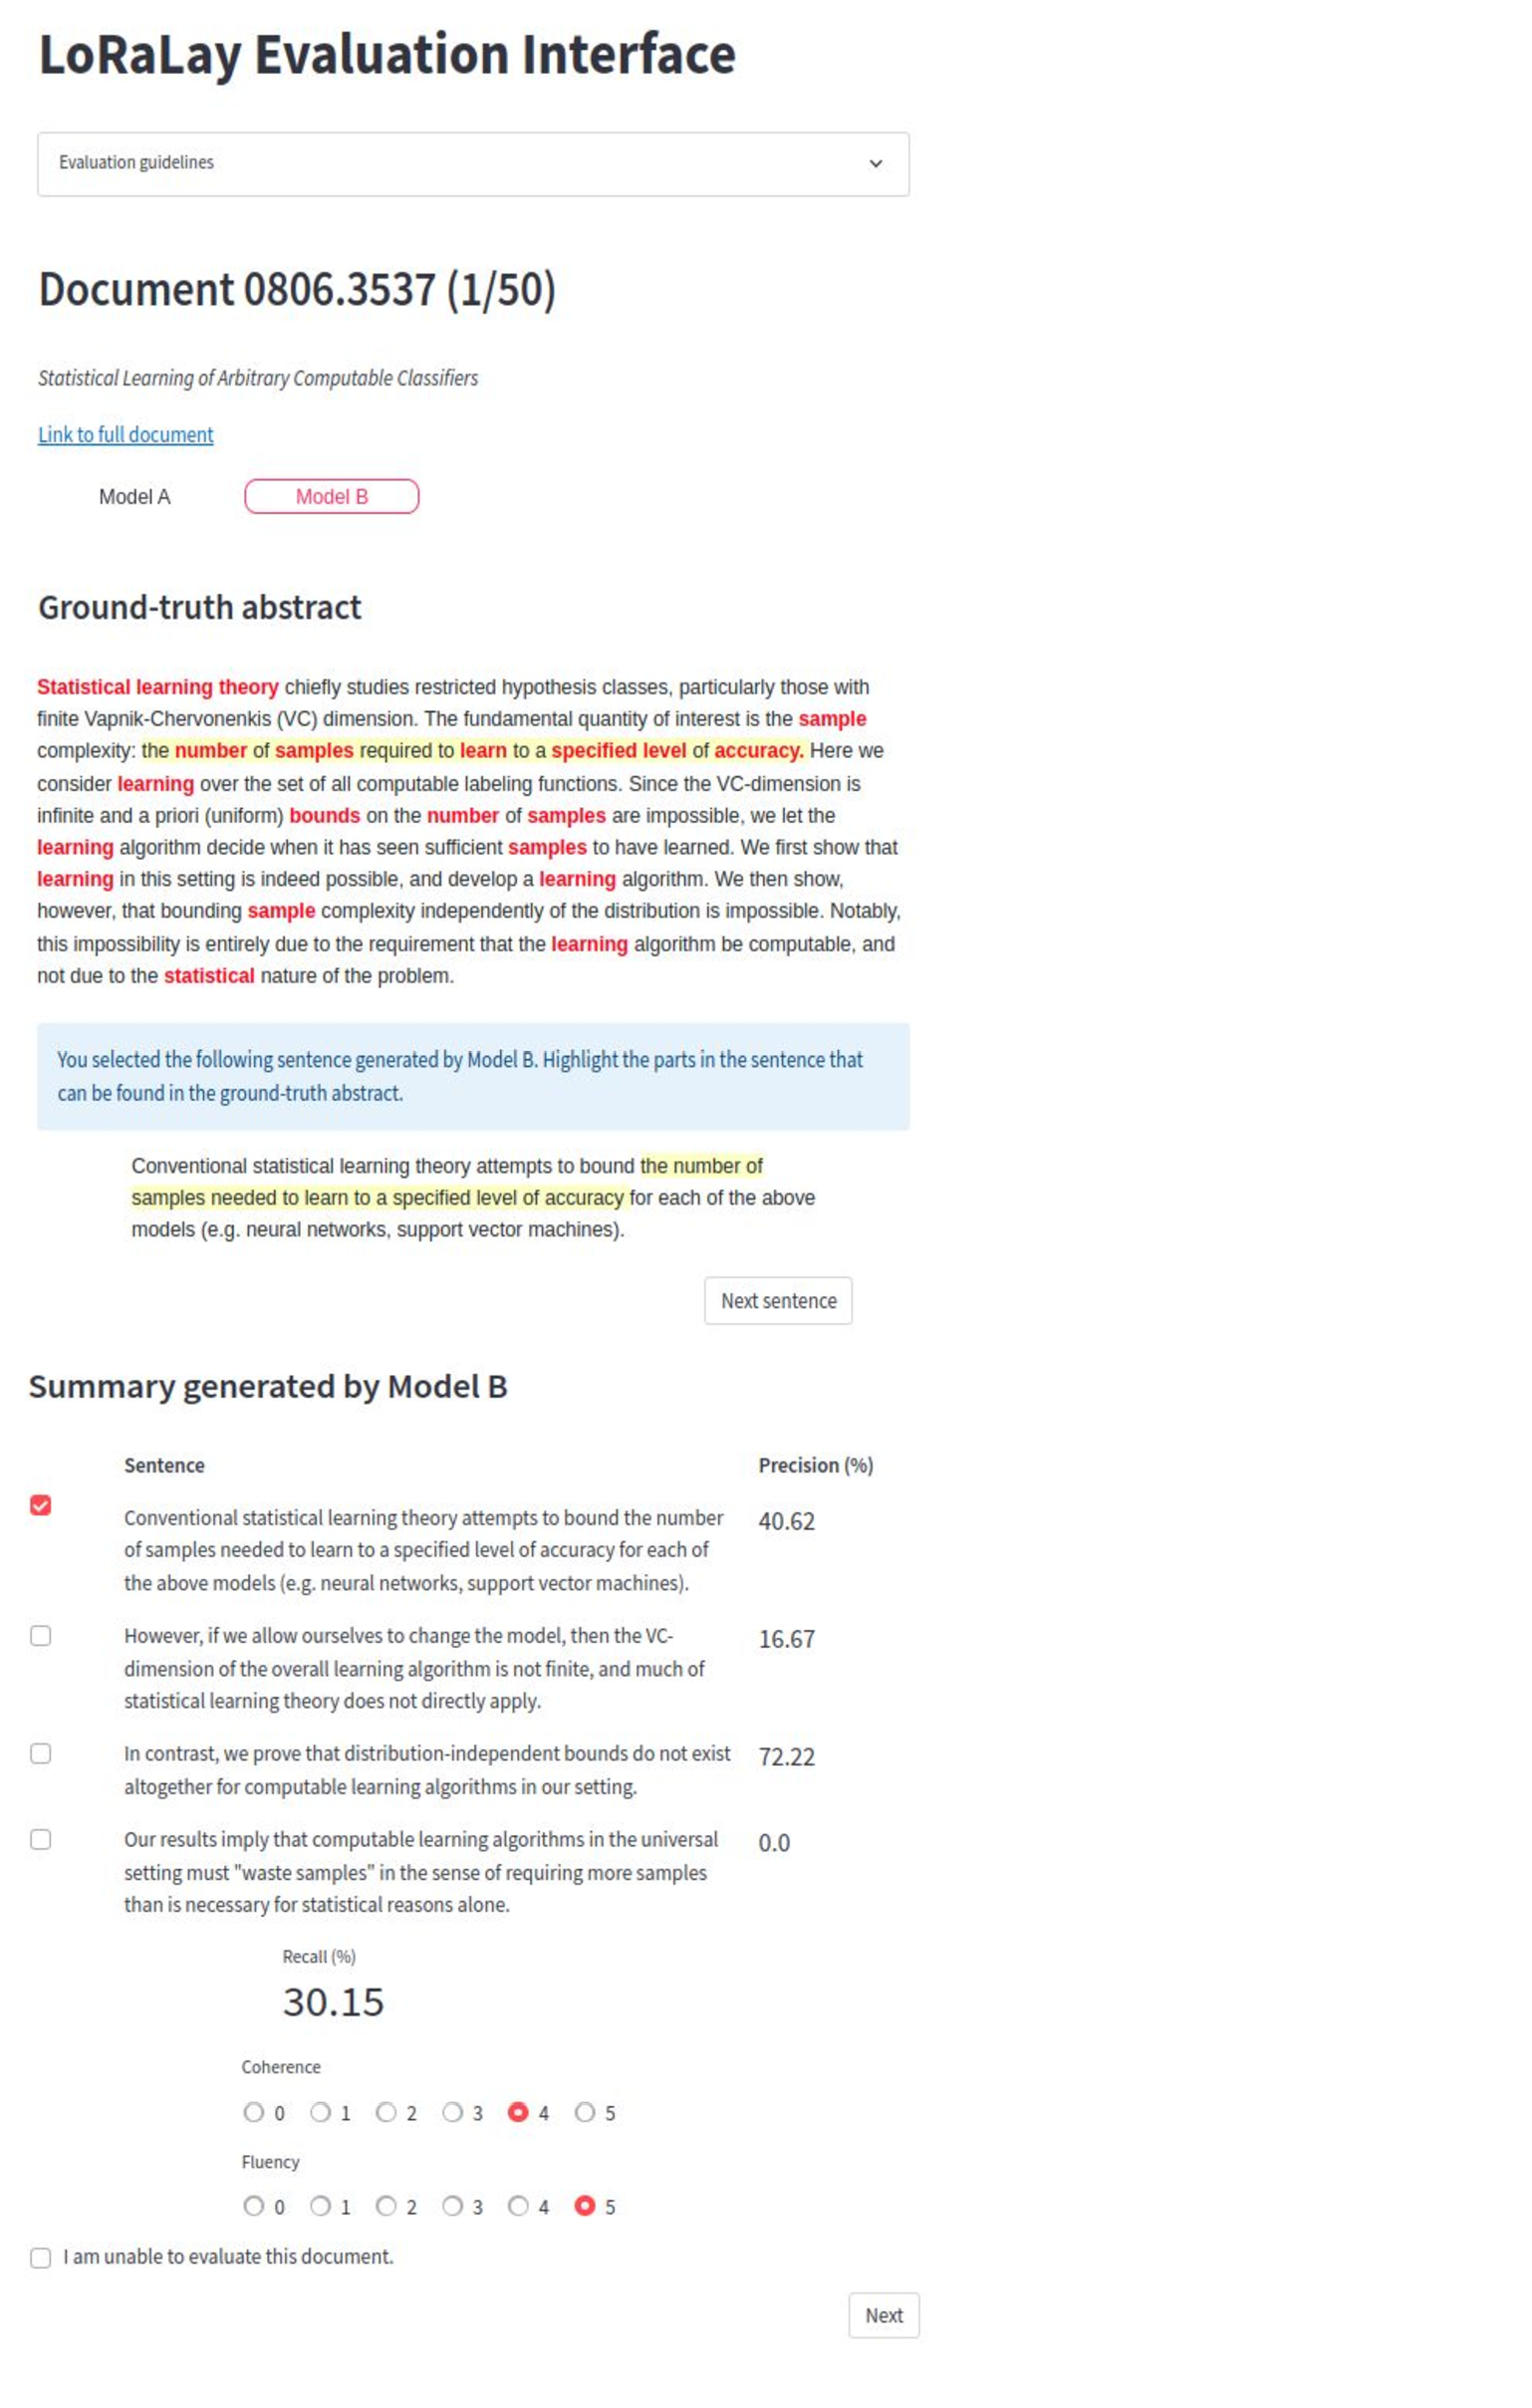
\includegraphics[width=0.6\textwidth]{images/chapter5/interface_preview.pdf}
  \caption{LoRaLay evaluation interface.}
  \label{fig:chapter5-loralay-eval-interface}
\end{figure}


\begin{table}[ht]
\centering
\small
\begin{tabular}{lccccc}
\toprule
\textbf{Metric}        & \textbf{BigBird} & \textbf{BigBird+Layout} \\ 
\midrule
Precision \%    &    35.15 \scriptsize{(0.81)}            &      37.51 \scriptsize{(0.70)}                   \\
Recall \%       &    28.07 \scriptsize{(0.73)}             &     33.59 \scriptsize{(0.86)}                   \\
Coherence     &     3.80 \scriptsize{(0.38)}             &      3.75 \scriptsize{(0.62)}                   \\ 
Fluency       &     4.48 \scriptsize{(0.03)}             &      4.34 \scriptsize{(0.16)}                   \\
Overlap \%     &    8.77 \scriptsize{(0.24)}             &     7.49 \scriptsize{(0.36)}                    \\ 
Flow \%             &   30.75 \scriptsize{(0.68)}          &    33.02 \scriptsize{(0.71)}                     \\
\bottomrule
\end{tabular}
\caption{Average human judgement scores obtained by comparing gold-truth abstracts and summaries generated by BigBird and BigBird+Layout from 50 documents sampled from arXiv-Lay and HAL. Inter-rater agreement	is computed using Krippendorff's alpha coefficient, and enclosed between parentheses.}
\label{tab:chapter5-human-eval-scores}
\end{table}

To gain more insight into the effect of document layout for summarizing long textual content, we conduct a human evaluation of summaries generated by BigBird-Pegasus/BigBird-MBART and their layout-aware counterparts. We choose the BigBird-based models over the LED ones, as the gain in augmenting BigBird with layout is much more apparent. We evenly sample 50 documents from arXiv-Lay and HAL test sets, filtering documents by their topics (computer science) to match the judgment capabilities of the three human annotators. 
Using the Streamlit\footnote{\url{https://streamlit.io/}} framework, we design and develop an interface to aid human evaluation of summarization models.\footnote{The code is publicly available at \url{https://anonymous.4open.science/r/loralay-eval-interface-C20D}.} A preview of the interface is presented in Figure~\ref{fig:chapter5-loralay-eval-interface}.
For each sentence $s_i$ in the generated summary, we ask the annotators to highlight the relevant tokens in $s_i$, along with the equivalent parts in the ground-truth abstract (denoted $h_i$). Further, we ask them to rate the summary in terms of coherence and fluency, on a scale of 0 to 5, following the DUC quality guidelines \citep{dang2005overview}. Finally, annotators are asked to penalize summaries with hallucinated facts. The highlighting process allows us to compute precision and recall as the percentage of highlighted information in the generated summary and the ground-truth abstract, respectively. Moreover, we can compute an overlap ratio as the percentage of highlighted information that appears several times in the generated summary. Lastly, we calculate a flow percentage that evaluates how well the order of the ground-truth information is preserved by computing the percentage of times where the highlighted text $h_i$ in the gold summary for one generated sentence $s_i$ follows the highlighted text $h_{i-1}$ for the previous sentence $s_{i-1}$ (i.e. where any token from $h_i$ occurs after a token in $h_{i-1}$).
Table~\ref{tab:chapter5-human-eval-scores} reports the scores for each metric and model, averaged over all 50 documents, along with inter-rater agreements, computed using Krippendorff's alpha coefficient. We find that adding layout to the models significantly improves precision and recall, results in less overlap (repetition), and is more in line with the ground truth order. Further, annotators did not encounter any hallucinated fact in the 50 generated summaries. To conclude, reported results show that human annotators strongly agree that adding layout generates better summaries, further validating our claim that layout provides vital information for summarization tasks.

\subsection{Case Studies}

\begin{figure}[ht]
    \centering
    \begin{subfigure}[b]{0.32\textwidth}
        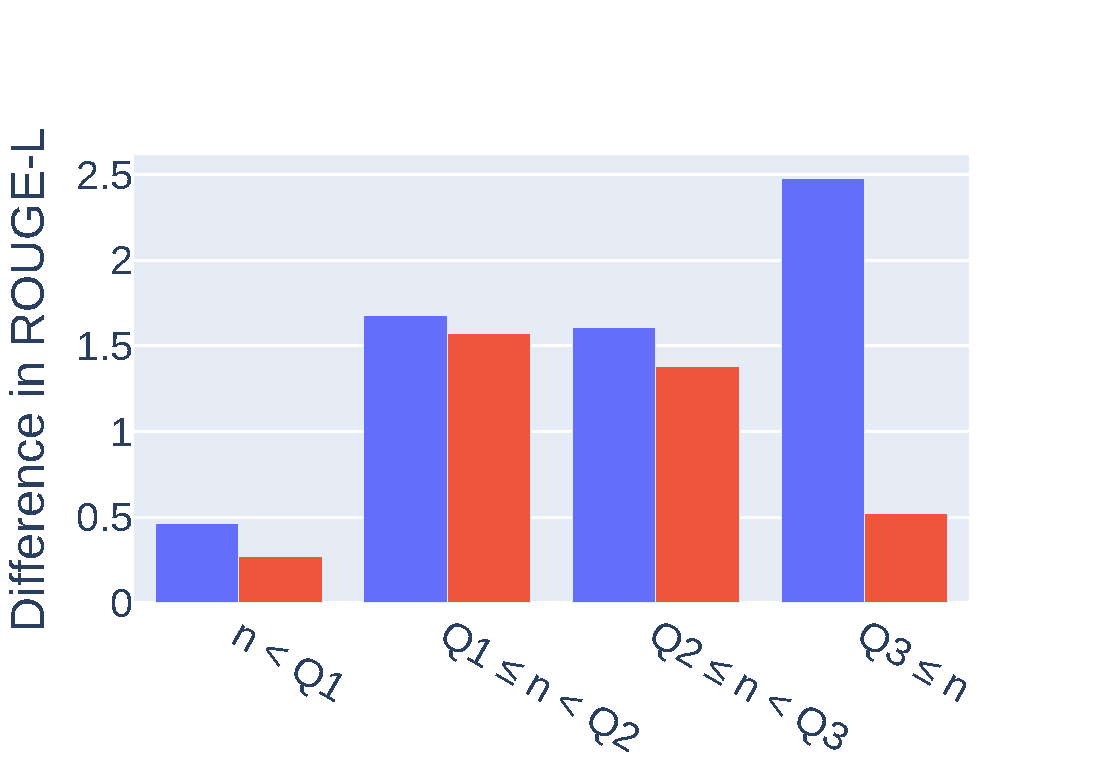
\includegraphics[width=1\textwidth]{images/chapter5/diff_in_len_barchart_nolegend.pdf}
        \caption{Article length}
    \end{subfigure}
    \begin{subfigure}[b]{0.32\textwidth}
        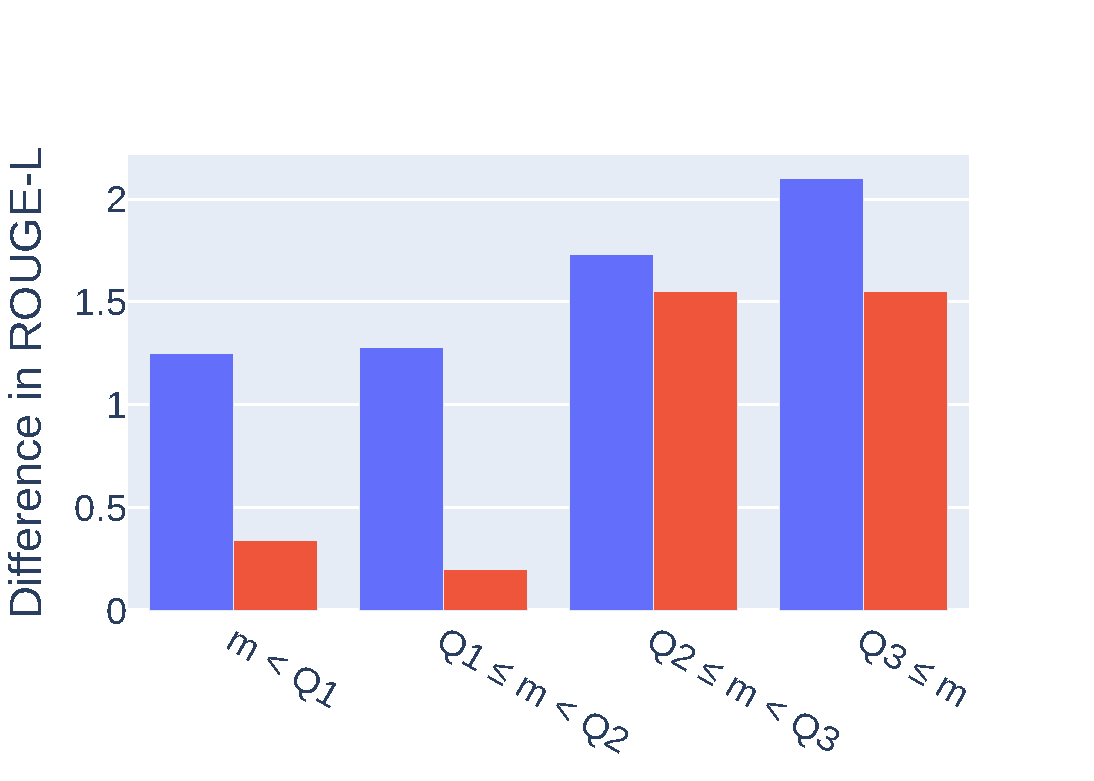
\includegraphics[width=\textwidth]{images/chapter5/diff_out_len_barchart_nolegend.pdf}
        \caption{Summary length}
    \end{subfigure}
    \begin{subfigure}[b]{0.32\textwidth}
        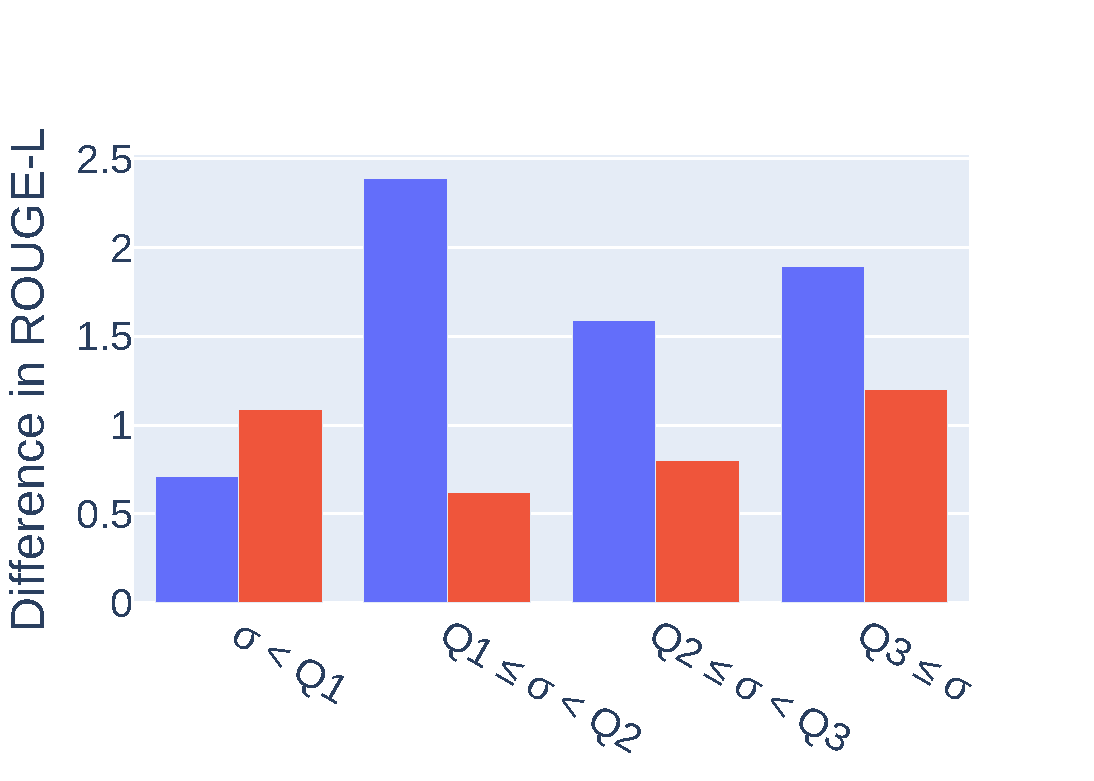
\includegraphics[width=\textwidth]{images/chapter5/diff_std_bbox_height_barchart_nolegend.pdf}
        \caption{$\sigma$ of bounding box height}
    \end{subfigure}
    \caption{Benefit of using layout on arXiv-Lay (blue) and PubMed-Lay (red), defined as the difference in ROUGE-L scores between BigBird-Pegasus+Layout and BigBird-Pegasus. For each dataset, quartiles are calculated from the distributions of article lengths (a), summary lengths (b) and variance in the height of the bounding boxes (c). ROUGE-L scores are then computed per quartile range, and averaged over each range.}
    \label{fig:chapter5-analysis-quartiles}
\end{figure}

\begin{table}[h]
\centering
\small
\resizebox{\linewidth}{!}{%
\begin{tabular}{crrrrrrrrr}
\toprule
\multirow{2}{*}{\textbf{Distribution}} & & \multicolumn{2}{c}{\textbf{Q1}} & & \multicolumn{2}{c}{\textbf{Q2}} & & \multicolumn{2}{c}{\textbf{Q3}} \\ \cline{3-4} \cline{6-7} \cline {9-10} 
               & & arXiv-Lay & PubMed-Lay & & arXiv-Lay & PubMed-Lay & & arXiv-Lay & PubMed-Lay \\ 
\midrule
Article Length                  & &    6,226 &    3,513 & &   9,142 &   5,557 & &   13,190 & 8,036 \\
Summary Length                  & &      119 &      130 & &     159 &     182 & &      202 &   247 \\  
$\sigma$ of bounding box height & &     3.37 &     1.34 & &    3.98 &    1.73 & &     4.70 &  2.28 \\
\bottomrule
      
\end{tabular}
}
\caption{Quartiles calculated from the distributions of article lengths, summary lengths, and variation in the height of bounding boxes, for arXiv-Lay and PubMed-Lay.}
\label{tab:chapter5-quartiles}
\end{table}

To have a better understanding of the previous results, we focus on uncovering the cases in which layout is most helpful. To this end, we identify features that relate to the necessity of having layout: 1) article length, as longer texts are intuitively easier to understand with layout, 2) summary length, as longer summaries are likely to cover more salient information, and 3) variance in font sizes (using the height of the bounding boxes), and, as such, the complexity of the layout.
The benefit of using layout is measured as the difference in ROUGE-L scores between BigBird-Pegasus+Layout and its purely textual counterpart, on arXiv-Lay and PubMed-Lay. We compute quartiles from the distributions of article lengths, ground-truth summary lengths, and variance in the height of bounding boxes. The quartiles are provided in Table~\ref{tab:chapter5-quartiles}. Based on the aforementioned factors, the scores obtained by each model are then grouped by quartile range, and averaged over each range, see Figure~\ref{fig:chapter5-analysis-quartiles}. On arXiv-Lay, we find that layout brings most improvement when dealing with the 25\% longest documents and summaries, while, for both datasets, layout is least beneficial for the shortest documents and summaries. These results corroborate our claim that layout can bring important information about long-range context. Concerning the third factor, we see, on PubMed-Lay, that layout is most helpful for documents that have the widest ranges of font sizes, showcasing the advantage of using layout to capture salient information. 

\section{Conclusion}

In this chapter, we have presented LoRaLay, a set of large-scale datasets for long-range and layout-aware text summarization. LoRaLay provides the research community with 4 novel multimodal corpora covering French, Spanish, Portuguese, and Korean languages, built from scientific articles. Furthermore, it includes additional layout and visual information for existing long-range summarization datasets (arXiv and PubMed). We provide adapted architectures merging layout-aware and long-range models, and show the importance of layout information in capturing long-range dependencies. Finally, we design an annotation interface for human evaluation of summaries, and introduce the flow metric.
	\cleardoublepage
	\let\leftmark=\oldleftmark

	\acresetall
	
\chapter{Conclusion}
\label{chapter:conclusion}

\acresetall
\acused{SHADE}

%\minitoc

We first summarize the contributions that we propose in this thesis before discussing interesting directions for future work. % that could be done in prolongation of those contributions.


	\cleardoublepage

	{
	\backmatter
	
\renewcommand{\leftmark}{\spacedlowsmallcaps{\bibname}}
\renewcommand{\rightmark}{\spacedlowsmallcaps{\bibname}}

\refstepcounter{dummy}
\addtocontents{toc}{\protect\vspace{\beforebibskip}} % to have the bib a bit from the rest in the toc
\addcontentsline{toc}{chapter}{\tocEntry{\bibname}}
\printbibliography

	\cleardoublepage
	}

	\appendix
	\acresetall
	\chapter{Appendix 1}
\adjustmtc
\label{chapter:App1}

\minitoc
\chapterwithfigures{\nameref*{chapter:App1}}
\chapterwithtables{\nameref*{chapter:App1}}

\vspace{2em}

\ifthenelse{\boolean{skipCh3}}{\endinput}{}


	\cleardoublepage

	\acresetall
	\chapter{Appendix 2}
\label{chapter:App2}

\ifthenelse{\boolean{skipCh4}}{\endinput}{}

\minitoc
\chapterwithfigures{\nameref*{chapter:App2}}
\chapterwithtables{\nameref*{chapter:App2}}

	\cleardoublepage

	\printbibliography

\end{document}
